
% This LaTeX was auto-generated from MATLAB code.
% To make changes, upda\textit{•}te the MATLAB code and republish this document.

\documentclass[a4paper, 11pt, twoside]{book}
\usepackage{graphicx}
\usepackage{color}
\usepackage[a4paper,left=2cm,right=2cm,top=2.5cm,bottom=2.5cm]{geometry}
%\sloppy
\definecolor{lightgray}{gray}{0.5}
\setlength{\parindent}{0pt}

\usepackage{amsmath}
 \usepackage{amssymb}
\usepackage{amsthm}

\usepackage[utf8]{inputenc}
\usepackage{verbatim}

\usepackage{fontspec}
\usepackage{fontenc}
\setmainfont[BoldFont={Minion Pro Semibold}, ItalicFont={Minion Pro Italic}]{Minion Pro}
\usepackage{titlesec}
   \newfontfamily\headingfont[]{Minion Pro Semibold}
  \titleformat{\chapter}[display]
  {\huge\headingfont}{\chaptertitlename\ \thechapter}{20pt}{\huge}
  
\usepackage{fancyvrb}
 
 \usepackage[pagebackref=true,breaklinks=true,letterpaper=true,colorlinks,bookmarks=false]{hyperref}

\usepackage[dvipsnames]{xcolor}
\hypersetup{
colorlinks,
linkcolor=black,
citecolor=black,
urlcolor=blue
}

\usepackage{float}

 \usepackage{fancyhdr}
 \pagestyle{fancy}
\fancyhead{}
\fancyhead[EL]{\leftmark}
\fancyhead[OR]{\rightmark}
%\lhead{Variational Gradient Matching for Dynamical Systems}
%\fancyfoot[L]{Version of \today}
\fancyfoot[C]{\thepage}

\begin{document}

  \begin{center}

{.}
  \vspace{1.2cm}

  \thispagestyle{empty}

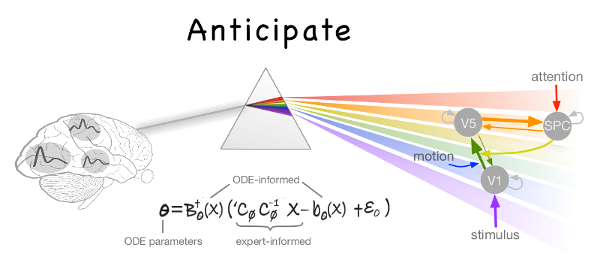
\includegraphics[width=5in]{logo.png}
\vspace{0.5cm}  

  {\LARGE\bf Code Documentation of Variational Gradient Matching \\ \vspace{0.3cm} for Dynamical Systems}
  
  \thispagestyle{empty}
             

%  Version of \today

  \vspace{1.2cm}

%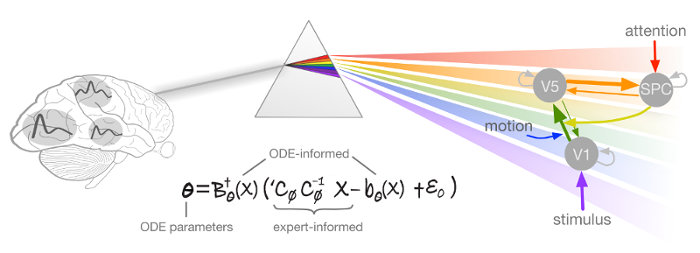
\includegraphics[width=6in]{cover_pic.png}
\end{center}
\vspace{2cm}
 {\Large \textbf{Authors}:\vspace{0.4cm}
\newline \textbf{Nico Stephan Gorbach} and \textbf{Stefan Bauer}, email: nico.gorbach@gmail.com}

\vspace{2cm}
{{\Large\textbf{Contents}:}\vspace{0.4cm}
\newline Code documentation for Variational Gradient Matching (VGM) described in the NIPS (2018) paper \href{https://papers.nips.cc/paper/7066-scalable-variational-inference-for-dynamical-systems.pdf}{Scalable Variational Inference for Dynamical Systems} by Nico S. Gorbach, Stefan Bauer and Joachim M. Buhmann (arxiv paper: \href{https://arxiv.org/pdf/1705.07079.pdf}{https://arxiv.org/pdf/1705.07079.pdf}). Please cite our paper if you use our program for a further publication. The derivations in this document are also given in the doctoral thesis \href{https://www.research-collection.ethz.ch/handle/20.500.11850/261734}{https://www.research-collection.ethz.ch/handle/20.500.11850/261734} as well as in parts of Wenk et al. (2018). Matlab code is illustrated in \color{RoyalPurple} purple \color{black} and the console output is illustrated in \color{MidnightBlue} blue\color{black}.

\vspace{0.3cm}
The code is available at \url{https://github.com/ngorbach/Variational_Gradient_Matching_for_Dynamical_Systems}. Online documentation of this code is available at \url{https://ngorbach.github.io/Variational_Gradient_Matching_for_Dynamical_Systems/#17}. In the repository, run one of the Matlab scripts\newline \textit{VGM\textunderscore for\textunderscore Lotka\textunderscore Volterra.m}, \textit{VGM\textunderscore for\textunderscore Lorenz96.m} and \textit{VGM\textunderscore for\textunderscore Lorenz\textunderscore attractor.m}. Alternatively, one can also run the live scripts \textit{VGM\textunderscore for\textunderscore Lotka\textunderscore Volterra\textunderscore live\textunderscore script.mlx}, \textit{VGM\textunderscore for\textunderscore Lorenz96\textunderscore live\textunderscore script.mlx} or\newline \textit{VGM\textunderscore for\textunderscore Lorenz\textunderscore Attractor\textunderscore live\textunderscore script.mlx}. The Matlab symbolic toolbox is required for this code.}




 \cleardoublepage 
 
\setcounter{tocdepth}{2}
\tableofcontents   
 
  \setcounter{chapter}{1}
\chapter*{VGM for Lotka-Volterra}
 \phantomsection\addcontentsline{toc}{chapter}{VGM for Lotka-Volterra}
Example dynamical system used in this code: \textbf{Lotka-Volterra} system with \textbf{half of the time points} \textbf{unobserved}. The ODE parameters are also unobserved.


\section{User Input}
\subsection{Simulation Settings}
\vspace{1em}
\begin{itemize}
   \item \textbf{true ODE parameter}: Input a row vector of real numbers of size 1 x 4:
    \color{RoyalPurple}\begin{verbatim}
simulation.ode_param = [2,1,4,1];
\end{verbatim}
\color{black}

   \item \textbf{final time for simulation}: Input a positive real number:
    \color{RoyalPurple}\begin{verbatim}
simulation.final_time = 2;
\end{verbatim}
\color{black}

   \item \textbf{observation noise}: Input a function handle:
    \color{RoyalPurple}\begin{verbatim}
simulation.state_obs_variance = @(mean)(bsxfun(@times,[0.5^2,0.5^2],...
ones(size(mean))));
\end{verbatim}
\color{black}

   \item \textbf{time interval between observations}: Input a positive real number:
    \color{RoyalPurple}\begin{verbatim}
simulation.interval_between_observations = 0.1;
\end{verbatim}
\color{black}
\end{itemize}

\vspace{1em}


\subsection{Estimation Settings}
\vspace{1em}
\begin{itemize}
   \item \textbf{Kernel Parameters} $\boldsymbol\phi$: Input a row vector of positive real numbers of size 1 x 2:
    \color{RoyalPurple}\begin{verbatim}
kernel.param = [10,0.2];
\end{verbatim}
\color{black}

   \item \textbf{Error variance on state derivatives (i.e. $\gamma$)}: Input a row vector of positive real numbers of size 1 x 2:
    \color{RoyalPurple}\begin{verbatim}
state.derivative_variance = [6,6];
\end{verbatim}
\color{black}

   \item \textbf{Estimation times}: Input a row vector of positive real numbers in ascending order:
    \color{RoyalPurple}\begin{verbatim}
time.est = 0:0.1:4;
\end{verbatim}
\color{black}
\end{itemize}
\vspace{2em}

\begin{par}
Preliminary operations
\end{par} \vspace{1em}
\color{RoyalPurple}\begin{verbatim}
close all; clc; addpath('VGM_functions')
\end{verbatim}
\color{black}


\section{Preprocessing}

\color{RoyalPurple}\begin{verbatim}
[symbols,simulation,ode,odes_path,coupling_idx,opt_settings,plot_settings] = ...
preprocessing_Lotka_Volterra (simulation);
\end{verbatim}

{\centering
\color{black}

        \color{MidnightBlue}\begin{verbatim} 
ODEs:
 
/ d x_1                                  \
| ----- == theta_1 x_1 - theta_2 x_1 x_2 |
|   dt                                   |
|                                        |
| d x_2                                  |
| ----- == theta_4 x_1 x_2 - theta_3 x_2 |
\   dt                                   /

\end{verbatim}

}
\color{black}


\section{Mass Action Dynamical Systems}

\begin{par}
A deterministic dynamical system is represented by a set of $K$ ordinary differential equations (ODEs) with model parameters $\boldsymbol\theta \in \mathbb{R}^d$ that describe the evolution of $K$ states $\mathbf{x}(t) = [x_1(t),\ldots, x_K(t)]^T$ such that:
\end{par} \vspace{1em}
\begin{par}
$\dot{\mathbf{x}}(t) = \frac{d \mathbf{x}(t)}{d t} = \mathbf{f}(\mathbf{x}(t),\boldsymbol\theta) \qquad (1)$,
\end{par} \vspace{1em}
\begin{par}
A sequence of observations, $\mathbf{y}(t)$, is usually contaminated by measurement error which we assume to be normally distributed with zero mean and variance for each of the $K$ states, i.e. $\mathbf{E}\sim\mathcal{N}(\mathbf{E};\mathbf{0},\mathbf{D})$, with $\mathbf{D}_{ik}=\sigma_k ^2 \delta_{ik}$. For $N$ distinct time points the overall system may therefore be summarized as
\end{par} \vspace{1em}
\begin{par}
$\mathbf{Y} = \mathbf{X} + \mathbf{E}$,
\end{par} \vspace{1em}
\begin{par}
where
\end{par} \vspace{1em}
\begin{par}
$\mathbf{X} = [\mathbf{x}(t_1),\ldots,\mathbf{x}(t_N)] =  [\mathbf{x}_1,\ldots,\mathbf{x}_K]^T$,
\end{par} \vspace{1em}
\begin{par}
$\mathbf{Y} = [\mathbf{y}(t_1),\ldots,\mathbf{y}(t_N)] =  [\mathbf{y}_1,\ldots,\mathbf{y}_K]^T$,
\end{par} \vspace{1em}
\begin{par}
and $\mathbf{x}_k = [x_k(t_1),\ldots,x_k(t_N)]^T$ is the $k$'th state sequence and $\mathbf{y}_k = [y_k(t_1),\ldots,y_k(t_N)]^T$ are the observations. Given the observations $\mathbf{Y}$ and the description of the dynamical system (1), the aim is to estimate both state variables $\mathbf{X}$ and parameters $\boldsymbol\theta$.
\end{par} \vspace{1em}
\begin{par}
We consider only dynamical systems that are \textit{locally linear} w.r.t. ODE parameters $\boldsymbol\theta$ and individual states $\mathbf{x}$. Such ODEs include mass-action kinetics and are given by:
\end{par} \vspace{1em}
\begin{par}
$f_{k}(\mathbf{x}(t),\theta) = \sum_{i=1} \theta_{k_i} \prod_{j \in\mathcal{M}_{k_i}} x_j \qquad (2)$,
\end{par} \vspace{1em}

\noindent with $\mathcal{M}_{k_i} \subseteq \{ 1, \dots, K\}$ describing the state variables in each factor of the equation (i.e. the functions are linear in parameters and contain arbitrary large products of monomials of the states).



\section{Simulate Trajectories}

\color{RoyalPurple}\begin{verbatim}
[simulation,obs_to_state_relation,fig_handle,plot_handle] = ...
simulate_state_dynamics(simulation,state,symbols,ode,odes_path,time,plot_settings);
\end{verbatim}
\color{black}

{\centering
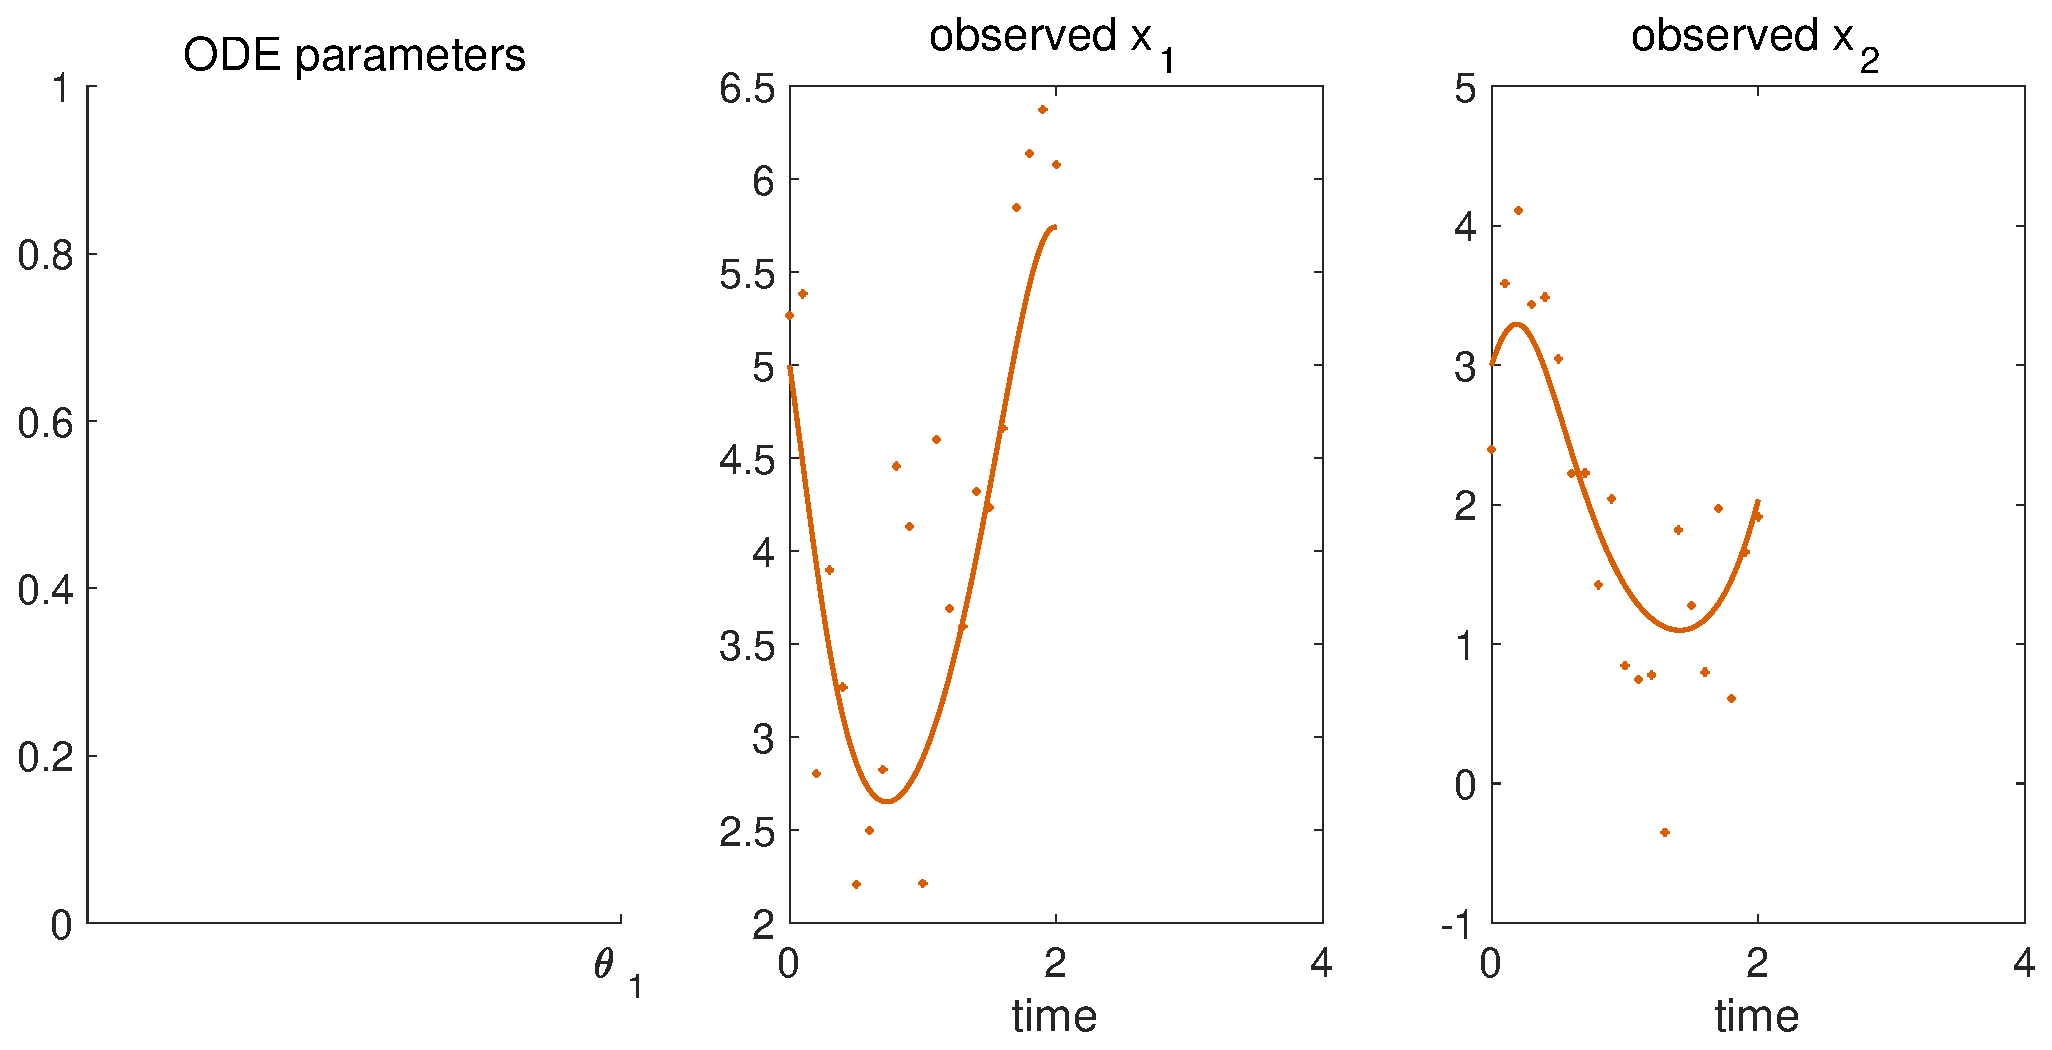
\includegraphics [width=5in]{VGM_for_Lotka_Volterra_01.eps}

}
\begin{par}
start timer
\end{par} \vspace{1em}
\color{RoyalPurple}\begin{verbatim}
tic;
\end{verbatim}
\color{black}


\section{Prior on States and State Derivatives}

\begin{par}
Gradient matching with Gaussian processes assumes a joint Gaussian process prior on states and their derivatives:
\end{par} \vspace{1em}
\begin{par}
$\left(\begin{array}{c} \mathbf{X} \\ \dot{\mathbf{X}} \end{array}\right) \sim \mathcal{N} \left(\begin{array}{c} \mathbf{X} \\ \dot{\mathbf{X}} \end{array}~;~\begin{array}{c} \mathbf{0} \\\mathbf{0} \end{array}~,~\begin{array}{cc} \mathbf{C}_{\boldsymbol\phi} & \mathbf{C}_{\boldsymbol\phi}' \\ '\mathbf{C}_\boldsymbol{\phi} & \mathbf{C}_{\boldsymbol\phi}'' \end{array} \right) \qquad (3)$,
\end{par} \vspace{1em}
\begin{par}
with
\end{par} \vspace{1em}
\begin{par}
$\mathrm{cov}(x_k(t), x_k(t)) = C_{\boldsymbol\phi_k}(t,t')$,
\end{par} \vspace{1em}
\begin{par}
$\mathrm{cov}(\dot{x}_k(t), x_k(t)) = \frac{\partial C_{\boldsymbol{\phi}_k}(t,t')}{\partial t} =: C_{{\boldsymbol\phi}_k}'(t,t')$,
\end{par} \vspace{1em}
\begin{par}
$\mathrm{cov}(x_k(t), \dot{x}_k(t)) = \frac{\partial C_{\boldsymbol\phi_k}(t,t')}{\partial t'} =: {'C_{\boldsymbol\phi_k}(t,t')}$,
\end{par} \vspace{1em}
\begin{par}
$\mathrm{cov}(\dot{x}_k(t), \dot{x}_k(t)) = \frac{\partial C_{\boldsymbol\phi_k}(t,t') }{\partial t \partial t'} =: C_{\boldsymbol\phi_k}''(t,t')$.
\end{par}


\section{Matching Gradients}

\begin{par}
Given the joint distribution over states and their derivatives (3) as well as the ODEs (2), we therefore have two expressions for the state derivatives:
\end{par} \vspace{1em}
\begin{par}
$\dot{\mathbf{X}} = \mathbf{F} + \boldsymbol\epsilon_1, \boldsymbol\epsilon_1 \sim\mathcal{N}\left(\boldsymbol\epsilon_1;\mathbf{0}, \mathbf{I}\gamma \right)$,
\end{par} \vspace{1em}
\begin{par}
$\dot{\mathbf{X}} = {'\mathbf{C}_{\boldsymbol\phi}} \mathbf{C}_{\boldsymbol\phi}^{-1}~\mathbf{X} + \boldsymbol\epsilon_2, \boldsymbol\epsilon_2 \sim\mathcal{N}\left(\boldsymbol\epsilon_2;\mathbf{0}, \mathbf{A} \right)$,
\end{par} \vspace{1em}
\begin{par}
where $\mathbf{F} := \mathbf{f}(\mathbf{X},\boldsymbol\theta)$ and $\mathbf{A} :=\mathbf{C}_{\boldsymbol\phi}'' -  {'\mathbf{C}_{\boldsymbol\phi}} \mathbf{C}_{\boldsymbol\phi}^{-1}\mathbf{C}_{\boldsymbol\phi}'$ and $\gamma$ is the error variance in the ODEs. Note that, in a deterministic system, the output of the ODEs $\mathbf{F}$ should equal the state derivatives $\dot{\mathbf{X}}$. However, in the first equation above we relax this constraint by adding stochasticity to the state derivatives $\dot{\mathbf{X}}$ in order to compensate for a potential model mismatch. The second equation above is obtained by deriving the conditional distribution for $\dot{\mathbf{X}}$ from the joint distribution in equation (3). Equating the two expressions in the equations above we can eliminate the unknown state derivatives $\dot{\mathbf{X}$:
\end{par} \vspace{1em}
\begin{par}
$\mathbf{F} = {'\mathbf{C}_{\boldsymbol\phi}} \mathbf{C}_{\boldsymbol\phi}^{-1} ~\mathbf{X} +\boldsymbol\epsilon_0 \qquad (4)$,
\end{par} \vspace{1em}
\begin{par}
with $\boldsymbol{\epsilon}_0 := \boldsymbol{\epsilon}_2 - \boldsymbol{\epsilon}_1$.
\end{par} \vspace{1em}
\color{RoyalPurple}\begin{verbatim}
[dC_times_invC,inv_C,A_plus_gamma_inv] = kernel_function(kernel,state,time.est);
\end{verbatim}
\color{black}


\section{Rewrite ODEs as Linear Combination in Parameters}

\begin{par}
Since, according to the mass action dynamics (equation 2), the ODEs are \textit{linear in the parameters} $\boldsymbol\theta$ we can rewrite the ODEs in equation (2) as a linear combination in the parameters:
\end{par} \vspace{1em}
\begin{par}
$\mathbf{B}_{\boldsymbol{\theta} k} \boldsymbol{\theta} + \mathbf{b}_{\boldsymbol{\theta} k} \stackrel{!}{=}\mathbf{f}_k(\mathbf{X},\boldsymbol{\theta}) \qquad (5)$,
\end{par} \vspace{1em}
\begin{par}
where matrices $\mathbf{B}_{\boldsymbol{\theta} k}$ and $\mathbf{b}_{\boldsymbol{\theta} k}$ are defined such that the ODEs $\mathbf{f}_k(\mathbf{X},\boldsymbol{\theta})$ are expressed as a linear combination in $\boldsymbol{\theta}$.
\end{par} 
\color{RoyalPurple}\begin{verbatim}
[ode_param.lin_comb.B,ode_param.lin_comb.b] = ...
rewrite_odes_as_linear_combination_in_parameters(ode,symbols);
\end{verbatim}
\color{black}


\section{Posterior over ODE Parameters}

\begin{par}
Inserting (5) into (4) and solving for $\boldsymbol{\theta}$ yields:
\end{par} \vspace{1em}
\begin{par}
$\boldsymbol{\theta} = \mathbf{B}_{\boldsymbol{\theta}}^+ \left( {'\mathbf{C}_{\boldsymbol{\phi}}}\mathbf{C}_{\boldsymbol{\phi}}^{-1} \mathbf{X} - \mathbf{b}_{\boldsymbol{\theta}} + \boldsymbol{\epsilon}_0\right)$,
\end{par} \vspace{1em}
\begin{par}
where $\mathbf{B}_{\boldsymbol{\theta}}^+$ denotes the pseudo-inverse of $\mathbf{B}_{\boldsymbol{\theta}}$. Since $\mathbf{C}_{\boldsymbol{\phi}}$ is block diagonal we can rewrite the expression above as:
\end{par} \vspace{1em}
\begin{par}
$\boldsymbol{\theta} = \left( \mathbf{B}_{\boldsymbol{\theta}}^T \mathbf{B}_{\boldsymbol{\theta}} \right)^{-1} ~\mathbf{B}_{\boldsymbol{\theta}}^T  \left( \sum_k {'\mathbf{C}_{\boldsymbol{\phi}_k}}\mathbf{C}_{\boldsymbol{\phi}_k}^{-1} \mathbf{X}_k - \mathbf{b}_{\boldsymbol{\theta} k} + \boldsymbol{\epsilon}_0^{(k)} \right)\\ ~= \left( \mathbf{B}_{\boldsymbol{\theta}}^T \mathbf{B}_{\boldsymbol{\theta}} \right)^{-1} \left(\sum_k \mathbf{B}_{\boldsymbol{\theta} k}^T \left( {'\mathbf{C}_{\boldsymbol{\phi}_k}}\mathbf{C}_{\boldsymbol{\phi}_k}^{-1} \mathbf{X}_k - \mathbf{b}_{\boldsymbol{\theta} k} +\boldsymbol{\epsilon}_0^{(k)} \right) \right)$,
\end{par} \vspace{1em}
\begin{par}
where we subsitute the Moore-Penrose inverse for the pseudo-inverse (i.e. $\mathbf{B}_{\boldsymbol{\theta}}^+ := \left( \mathbf{B}_{\boldsymbol{\theta}}^T \mathbf{B}_{\boldsymbol{\theta}}\right)^{-1} \mathbf{B}_{\boldsymbol{\theta}}^T$). We can therefore derive the posterior distribution over ODE parameters:
\end{par} \vspace{1em}
\begin{par}
$p(\boldsymbol{\theta} \mid \mathbf{X}, \boldsymbol{\phi}, \gamma) = \mathcal{N}\left(\boldsymbol{\theta} ; \left( \mathbf{B}_{\boldsymbol{\theta}}^T\mathbf{B}_{\boldsymbol{\theta}} \right)^{-1} \left( \sum_k \mathbf{B}_{\boldsymbol{\theta} k}^T ~\left( {'\mathbf{C}_{\boldsymbol{\phi} k}} \mathbf{C}_{\boldsymbol{\phi} k}^{-1} \mathbf{X}_k -\mathbf{b}_{\boldsymbol{\theta} k} \right) \right), ~ \mathbf{B}_{\boldsymbol{\theta}}^+ ~(\mathbf{A} + \mathbf{I}\gamma) ~ \mathbf{B}_{\boldsymbol{\theta}}^{+T}\right) \qquad (6)$.
\end{par} \vspace{1em}


\section{Rewrite ODEs as Linear Combination in Individual States}

\begin{par}
Since, according to the mass action dynamics (equation 2), the ODEs are \textit{linear in the individual state} $\mathbf{x}_u$ we can rewrite the ODE $\mathbf{f}_k(\mathbf{X},\boldsymbol\theta)$ as a linear combination in the individual state $\mathbf{x}_u$:
\end{par} \vspace{1em}
\begin{par}
$\mathbf{R}_{uk} \mathbf{x}_u + \mathbf{r}_{uk} \stackrel{!}{=}\mathbf{f}_k(\mathbf{X},\boldsymbol{\theta})$,
\end{par} \vspace{1em}
\begin{par}
where matrices  $\mathbf{R}_{uk}$ and  $\mathbf{r}_{uk}$ are defined such that the ODE $\mathbf{f}_k(\mathbf{X},\boldsymbol{\theta})$ is expressed as a linear combination in the individual state $\mathbf{x}_u$.
\end{par} \vspace{1em}
\color{RoyalPurple}\begin{verbatim}
[state.lin_comb.R,state.lin_comb.r] = ...
rewrite_odes_as_linear_combination_in_ind_states(ode,symbols,coupling_idx.states);
\end{verbatim}
\color{black}


\section{Posterior over Individual States}

\begin{par}
Given the linear combination of the ODEs w.r.t. an individual state, we define the matrices $\mathbf{B}_u$ and $\mathbf{b}_u$ such that the expression $\mathbf{f}(\mathbf{X},\boldsymbol{\theta}) - {'\mathbf{C}}_{\boldsymbol{\phi}}\mathbf{C}_{\boldsymbol{\phi}}^{-1} \mathbf{X}$ is rewritten as a linear combination in an individual state $\mathbf{x}_u$:
\end{par} \vspace{1em}
\begin{par}
$\mathbf{B}_{u} \mathbf{x}_u + \mathbf{b}_{u} \stackrel{!}{=}\mathbf{f}(\mathbf{X},\boldsymbol{\theta}) - {'\mathbf{C}}_{\boldsymbol{\phi}}\mathbf{C}_{\boldsymbol{\phi}}^{-1} \mathbf{X} \qquad (7)$.
\end{par} \vspace{1em}
\begin{par}
Inserting (7) into (4) and solving for $\mathbf{x}_u$ yields:
\end{par} \vspace{1em}
\begin{par}
$\mathbf{x}_u = \mathbf{B}_{u}^+ \left( \boldsymbol{\epsilon}_0 -\mathbf{b}_{u}\right)$,
\end{par} \vspace{1em}
\begin{par}
where $\mathbf{B}_{u}^+$ denotes the pseudo-inverse of $\mathbf{B}_{u}$. Since $\mathbf{C}_{\boldsymbol{\phi}}$ is block diagonal we can rewrite the expression above as:
\end{par} \vspace{1em}
\begin{par}
$\mathbf{x}_u = \left( \mathbf{B}_{u} \mathbf{B}_{u}^T \right)^{-1}\mathbf{B}_{u}^T \sum_k \left(\boldsymbol{\epsilon}_0^{(k)} -\mathbf{b}_{uk} \right)\\ \quad= \left( \mathbf{B}_{u} \mathbf{B}_{u}^T \right)^{-1} \sum_k\mathbf{B}_{uk}^T \left(\boldsymbol{\epsilon}_0^{(k)} -\mathbf{b}_{uk} \right)$,
\end{par} \vspace{1em}
\begin{par}
where we substitute the Moore-Penrose inverse for the pseudo-inverse (i.e. $\mathbf{B}_{\boldsymbol{\theta}}^+ := \left( \mathbf{B}_{\boldsymbol{\theta}}^T \mathbf{B}_{\boldsymbol{\theta}}\right)^{-1} \mathbf{B}_{\boldsymbol{\theta}}^T$).  We can therefore derive the posterior distribution over an individual state $\mathbf{x}_{u}$:
\end{par} \vspace{1em}
\begin{par}
$p(\mathbf{x}_u \mid \mathbf{X}_{-u}, \boldsymbol{\phi}, \gamma)= \mathcal{N}\left(\mathbf{x}_u ; \left( \mathbf{B}_{u} \mathbf{B}_{u}^T\right)^{-1} \left( - \sum_k \mathbf{B}_{uk}^T \mathbf{b}_{uk} \right),~\mathbf{B}_{u}^{+} ~ (\mathbf{A} + \mathbf{I}\gamma) ~ \mathbf{B}_u^{+T}\right) \qquad (8)$,
\end{par} \vspace{1em}
\begin{par}
with $\mathbf{X}_{-u}$ denoting the set of all states except state $\mathbf{x}_u$.
\end{par} \vspace{1em}


\section{Mean-field Variational Inference}

\begin{par}
To infer the parameters $\boldsymbol{\theta}$, we want to find the maximum a posteriori estimate (MAP):
\end{par} \vspace{1em}
\begin{par}
$\boldsymbol{\theta}^* := \mathrm{arg} \max_{\boldsymbol{\theta}} ~ \ln p(\boldsymbol{\theta} \mid\mathbf{Y},\boldsymbol{\phi},\gamma,\mathbf \sigma)\\ \quad= \mathrm{arg}\max_{\boldsymbol{\theta}} ~ \ln \int  p(\boldsymbol{\theta},\mathbf{X} \mid\mathbf{Y},\boldsymbol{\phi},\gamma,\boldsymbol\sigma) d\mathbf{X}\\ \quad= \mathrm{arg}\max_{\boldsymbol{\theta}} ~ \ln \int p(\boldsymbol{\theta} \mid \mathbf{X},\boldsymbol{\phi},\gamma)p(\mathbf{X} \mid \mathbf{Y}, \boldsymbol{\phi},\boldsymbol\sigma) d\mathbf{X} \qquad(9)$.
\end{par} \vspace{1em}
\begin{par}
However, the integral above is intractable due to the strong couplings induced by the nonlinear ODEs $\mathbf{f}$ which appear in the term $p(\boldsymbol{\theta} \mid \mathbf{X},\boldsymbol{\phi},\gamma)$.
\end{par} \vspace{1em}
\begin{par}
We use mean-field variational inference to establish variational lower bounds that are analytically tractable by decoupling state variables from the ODE parameters as well as decoupling the state variables from each other. Note that, since the ODEs described by equation (2) are \textit{locally linear}, both conditional distributions $p(\boldsymbol{\theta} \mid\mathbf{X},\mathbf{Y},\boldsymbol{\phi},\gamma,\boldsymbol\sigma)$ (equation (6)) and $p(\mathbf{x}_u \mid \boldsymbol{\theta},\mathbf{X}_{-u},\mathbf{Y},\boldsymbol{\phi},\gamma,\boldsymbol\sigma)$ (equation (8)) are analytically tractable and Gaussian distributed as mentioned previously. The decoupling is induced by designing a variational distribution $Q(\boldsymbol{\theta},\mathbf{X})$ which is restricted to the family of factorial distributions:
\end{par} \vspace{1em}
\begin{par}
$\mathcal{Q} := \bigg{\{} Q : Q(\boldsymbol{\theta},\mathbf{X}) = q(\boldsymbol{\theta}) \prod_uq(\mathbf{x}_u) \bigg{\}}$.
\end{par} \vspace{1em}
\begin{par}
The particular form of $q(\boldsymbol{\theta})$ and $q(\mathbf{x}_u)$ are designed to be Gaussian distributed which places them in the same family as the true full conditional distributions. To find the optimal factorial distribution we minimize the Kullback-Leibler divergence between the variational and the true posterior distribution:
\end{par} \vspace{1em}
\begin{par}
$\hat{Q} := \mathrm{arg} \min_{Q(\boldsymbol{\theta},\mathbf{X}) \in \mathcal{Q}} \mathrm{KL}\left[ Q(\boldsymbol{\theta},\mathbf{X}) \mid \mid p(\boldsymbol{\theta},\mathbf{X} \mid\mathbf{Y},\boldsymbol{\phi}, \gamma,\mathbf\boldsymbol{\sigma}) \right] \qquad (10)$,
\end{par} \vspace{1em}
\begin{par}
where $\hat{Q}$ is the proxy distribution. The proxy distribution that minimizes the KL-divergence (10) depends on the true full conditionals and is given by:
\end{par} \vspace{1em}
\begin{par}
$\hat{q}({\boldsymbol{\theta}}) \propto \exp \left(~ E_{Q_{-\boldsymbol{\theta}}} \ln p(\boldsymbol{\theta} \mid\mathbf{X},\mathbf{Y},\boldsymbol{\phi},\gamma,\mathbf\boldsymbol{\sigma}) ~\right) \qquad (11)\\\hat{q}(\mathbf{x}_u) \propto \exp\left( ~ E_{Q_{-u}} \ln p(\mathbf{x}_u\mid \boldsymbol{\theta}, \mathbf{X}_{-u},\mathbf{Y},\boldsymbol{\phi},\gamma,\boldsymbol{\sigma}) ~ \right)\qquad (12)$.
\end{par} \vspace{1em}


\section{Fitting Observations of State Trajectories}

\begin{par}
We fit the observations of state trajectories by standard GP regression. The data-informed distribution $p(\mathbf{X} \mid \mathbf{Y}, \boldsymbol{\phi},\mathbf\boldsymbol{\sigma})$ in euqation (9) can be determined analytically using Gaussian process regression with the GP prior $p(\mathbf{X} \mid\boldsymbol{\phi}) = \prod_k \mathcal{N}(\mathbf{x}_k ;\mathbf{0},\mathbf{C}_{\boldsymbol{\phi}_k})$:
\end{par} \vspace{1em}
\begin{par}
$p(\mathbf{X} \mid \mathbf{Y}, \boldsymbol{\phi},\gamma) = \prod_k\mathcal{N}(\mathbf{x}_k ;\boldsymbol\mu_k(\mathbf{y}_k),\mathbf\boldsymbol{\sigma}_k)$,
\end{par} \vspace{1em}
\begin{par}
where $\boldsymbol\mu_k(\mathbf{y}_k) := \boldsymbol{\sigma}_k^{-2} \left(\boldsymbol{\sigma}_k^{-2}\mathbf{I} + \mathbf{C}_{\boldsymbol{\phi}_k}^{-1} \right)^{-1} \mathbf{y}_k$ and $\boldsymbol{\sigma}_k ^{-1}:=\boldsymbol{\sigma}_k^{-2} \mathbf{I} +\mathbf{C}_{\mathbf\boldsymbol{\phi}_k}^{-1}$.
\end{par} \vspace{1em}
\color{RoyalPurple}\begin{verbatim}
[mu,inv_sigma] = fitting_state_observations(inv_C,obs_to_state_relation,...
simulation,symbols);
\end{verbatim}
\color{black}


\section{Coordinate Ascent Variational Gradient Matching}

\begin{par}
We minimize the KL-divergence in equation (10) by coordinate descent (where each step is analytically tractable) by iterating between determining the proxy for the distribution over ODE parameters $\hat{q}(\boldsymbol{\theta})$ and the proxies for the distribution over individual states $\hat{q}(\mathbf{x}_u)$.
\end{par}

\vspace{1.5em}
\textbf{Initialize the state estimation by the GP regression posterior}

\color{RoyalPurple}\begin{verbatim}
state.proxy.mean = array2table([time.est',mu],...
'VariableNames',['time',symbols.state_string]);
\end{verbatim}
\color{black}
\begin{par}

\end{par} \vspace{1.5em}

\textbf{Coordinate ascent}

\color{RoyalPurple}\begin{verbatim}
for i = 1:opt_settings.coord_ascent_numb_iter
\end{verbatim}
\color{black}

\subsection{Proxy for ODE parameters}


\begin{par}
Expanding the proxy distribution in equation (11) for $\boldsymbol{\theta}$ yields:
\end{par} \vspace{1em}

\begin{par}
$\hat{q}(\mathbf{\boldsymbol\theta}) \propto \exp
\left( ~E_{Q_{-\boldsymbol\theta}}     \ln p(\boldsymbol\theta \mid \mathbf{X},\mathbf{Y},\boldsymbol\phi,\gamma,\boldsymbol\sigma)
~     \right) \\ \qquad= \exp \left( ~E_{Q_{-\boldsymbol{\theta}}} \ln \mathcal{N}\left(\boldsymbol{\theta}
; \left(    \mathbf{B}_{\boldsymbol{\theta}}^T \mathbf{B}_{\boldsymbol{\theta}} \right)^{-1}
\left( \sum_k    \mathbf{B}_{\boldsymbol{\theta} k}^T ~ \left( {'\mathbf{C}_{\boldsymbol{\phi}
k}}    \mathbf{C}_{\boldsymbol{\phi} k}^{-1} \mathbf{X}_k - \mathbf{b}_{\boldsymbol{\theta}
k} \right)    \right), ~ \mathbf{B}_{\boldsymbol{\theta}}^+ ~ (\mathbf{A} + \mathbf{I}\gamma)
~    \mathbf{B}_{\boldsymbol{\theta}}^{+T} \right) ~\right)$,
\end{par} \vspace{1em}

where we substitute $p(\boldsymbol{\theta} \mid \mathbf{X},\boldsymbol{\phi},\gamma)$ with its density given in equation (6).
    \color{RoyalPurple}\begin{verbatim}
             [param_proxy_mean,param_proxy_inv_cov] = ...
             proxy_for_ode_parameters(state.proxy.mean{:,symbols.state_string},...
                    dC_times_invC,ode_param.lin_comb,symbols,A_plus_gamma_inv,opt_settings);
\end{verbatim}
\color{black}
\begin{par}
Intermediate results
\end{par} \vspace{1em}
\color{RoyalPurple}\begin{verbatim}
            if i==1 || ~mod(i,1)
                plot_results(fig_handle,state.proxy,simulation,param_proxy_mean,...
                plot_handle,symbols,plot_settings,'not_final');
            end
\end{verbatim}
\color{black}

{\centering
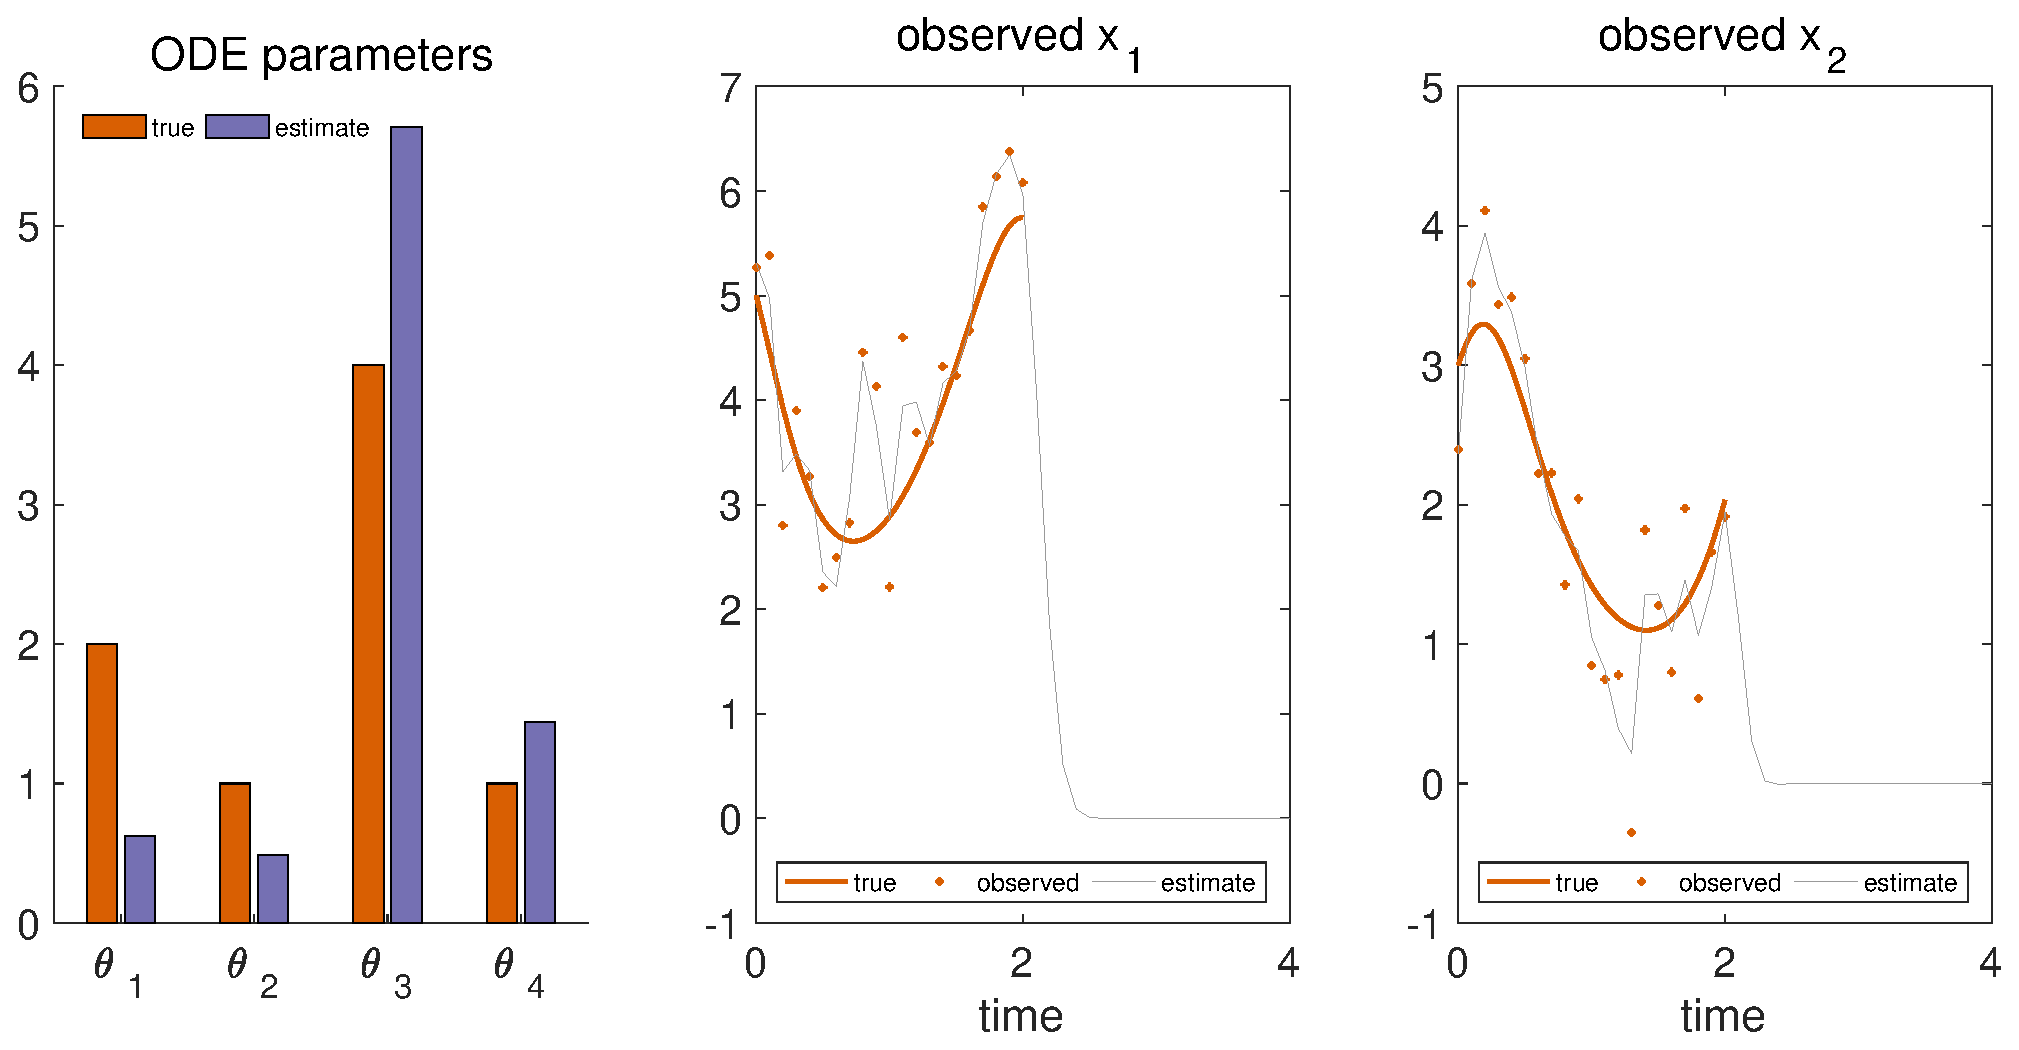
\includegraphics [width=5in]{VGM_for_Lotka_Volterra_02.eps}

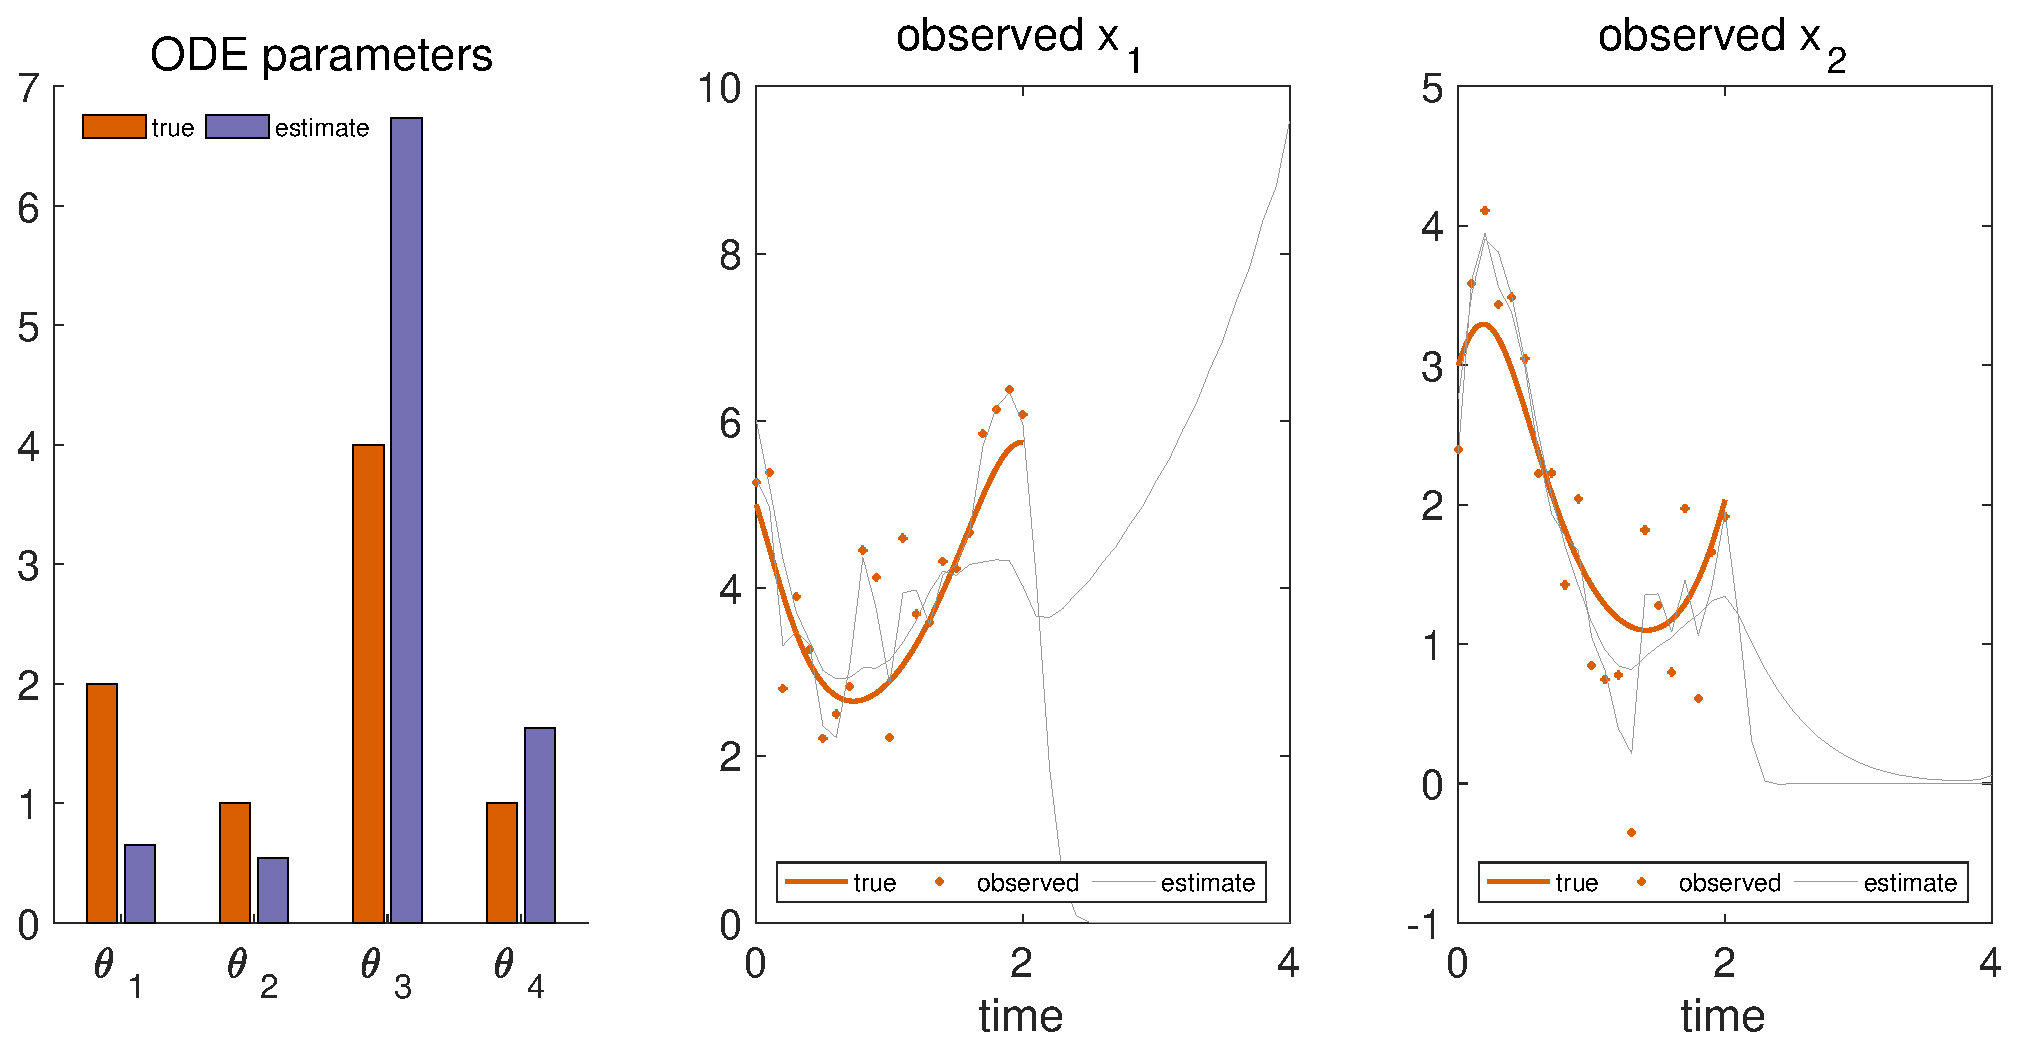
\includegraphics [width=5in]{VGM_for_Lotka_Volterra_03.eps}

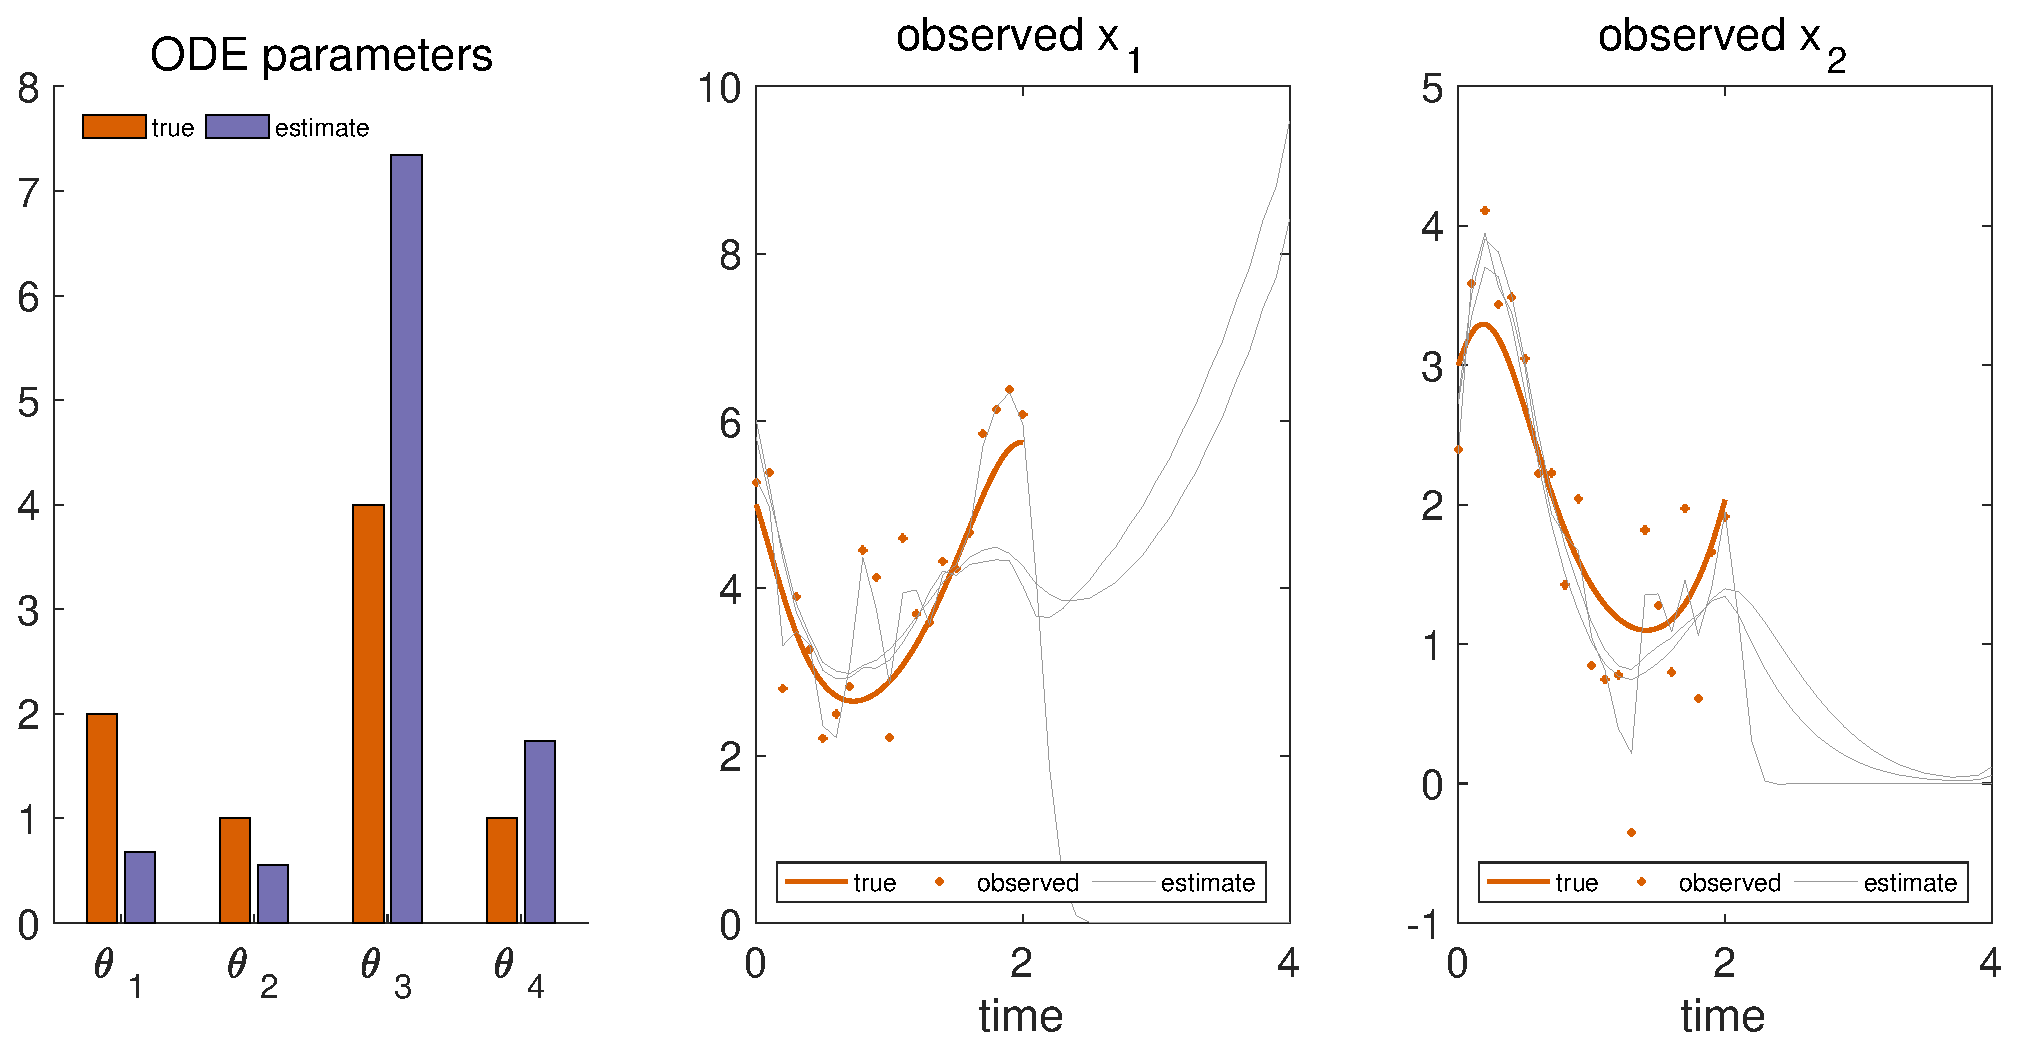
\includegraphics [width=5in]{VGM_for_Lotka_Volterra_04.eps}

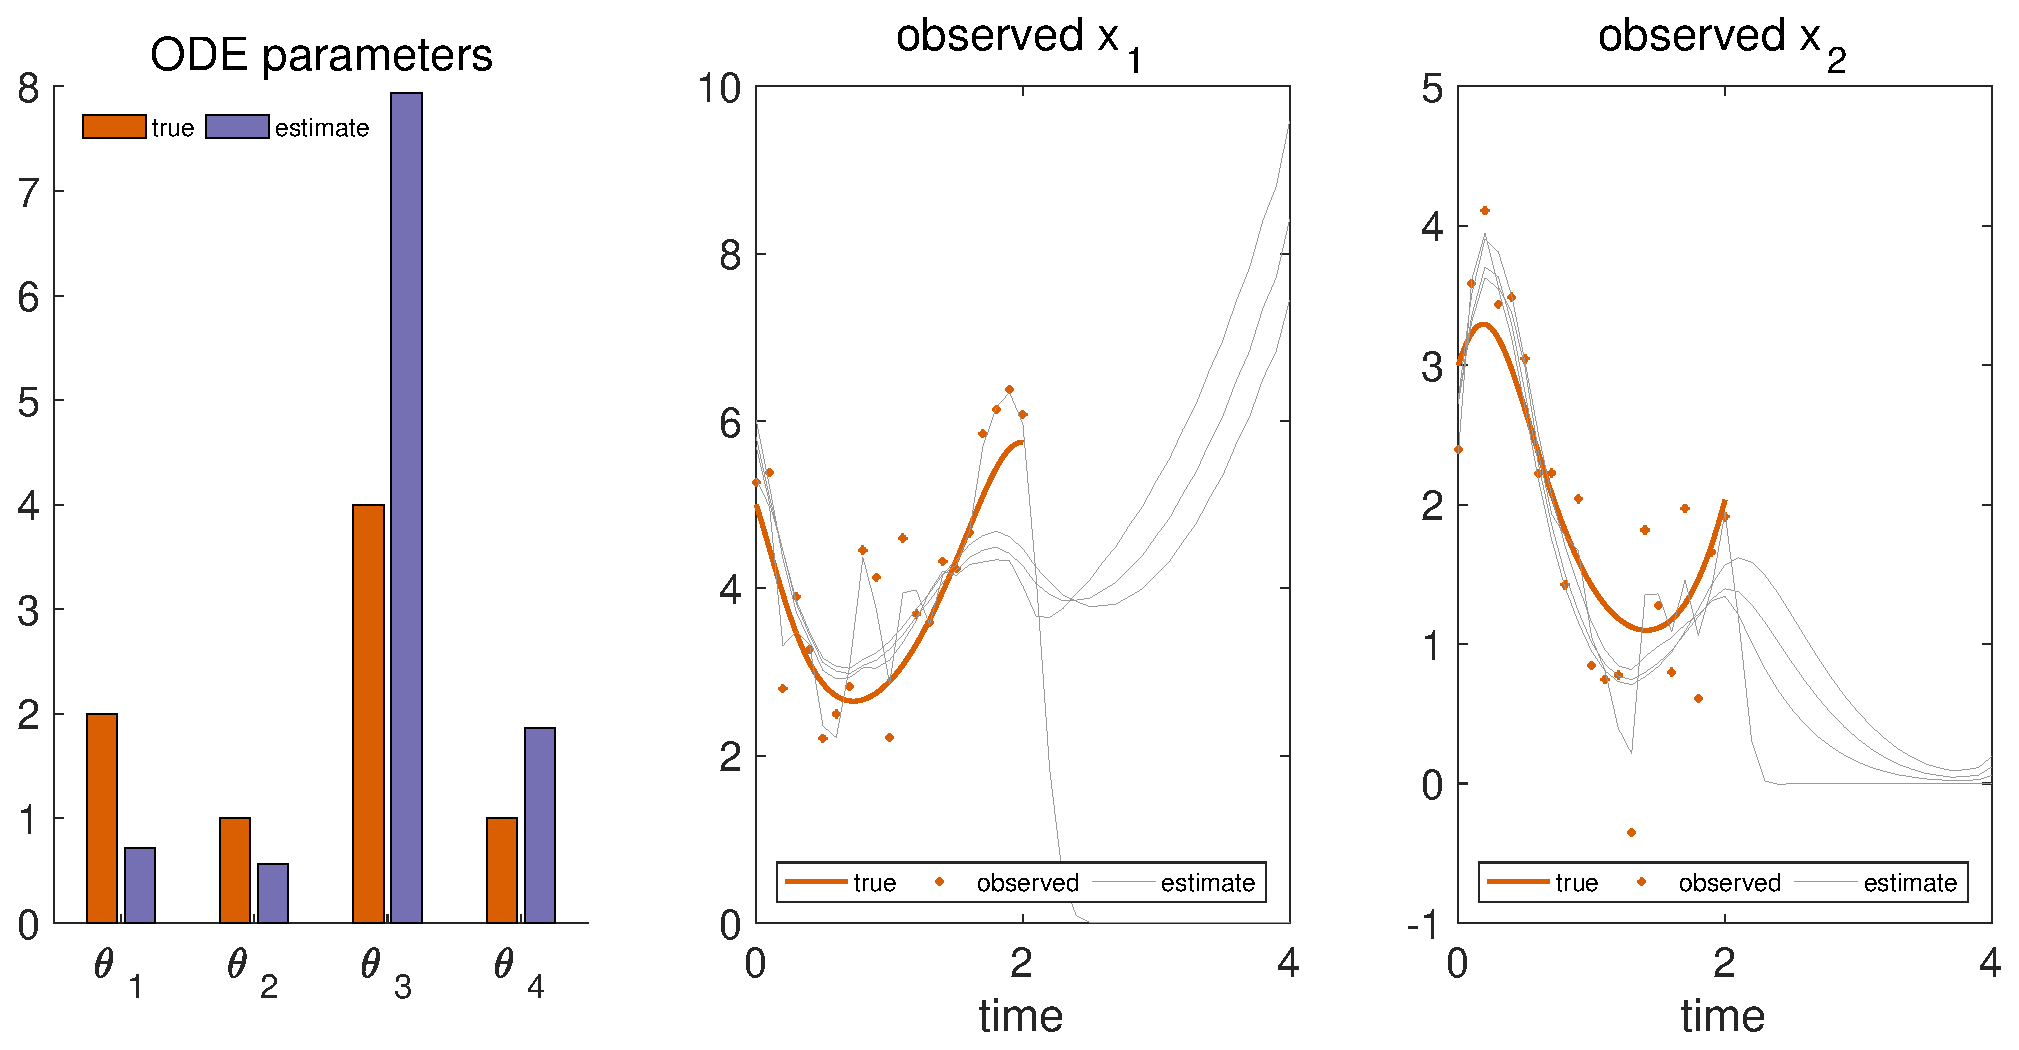
\includegraphics [width=5in]{VGM_for_Lotka_Volterra_05.eps}

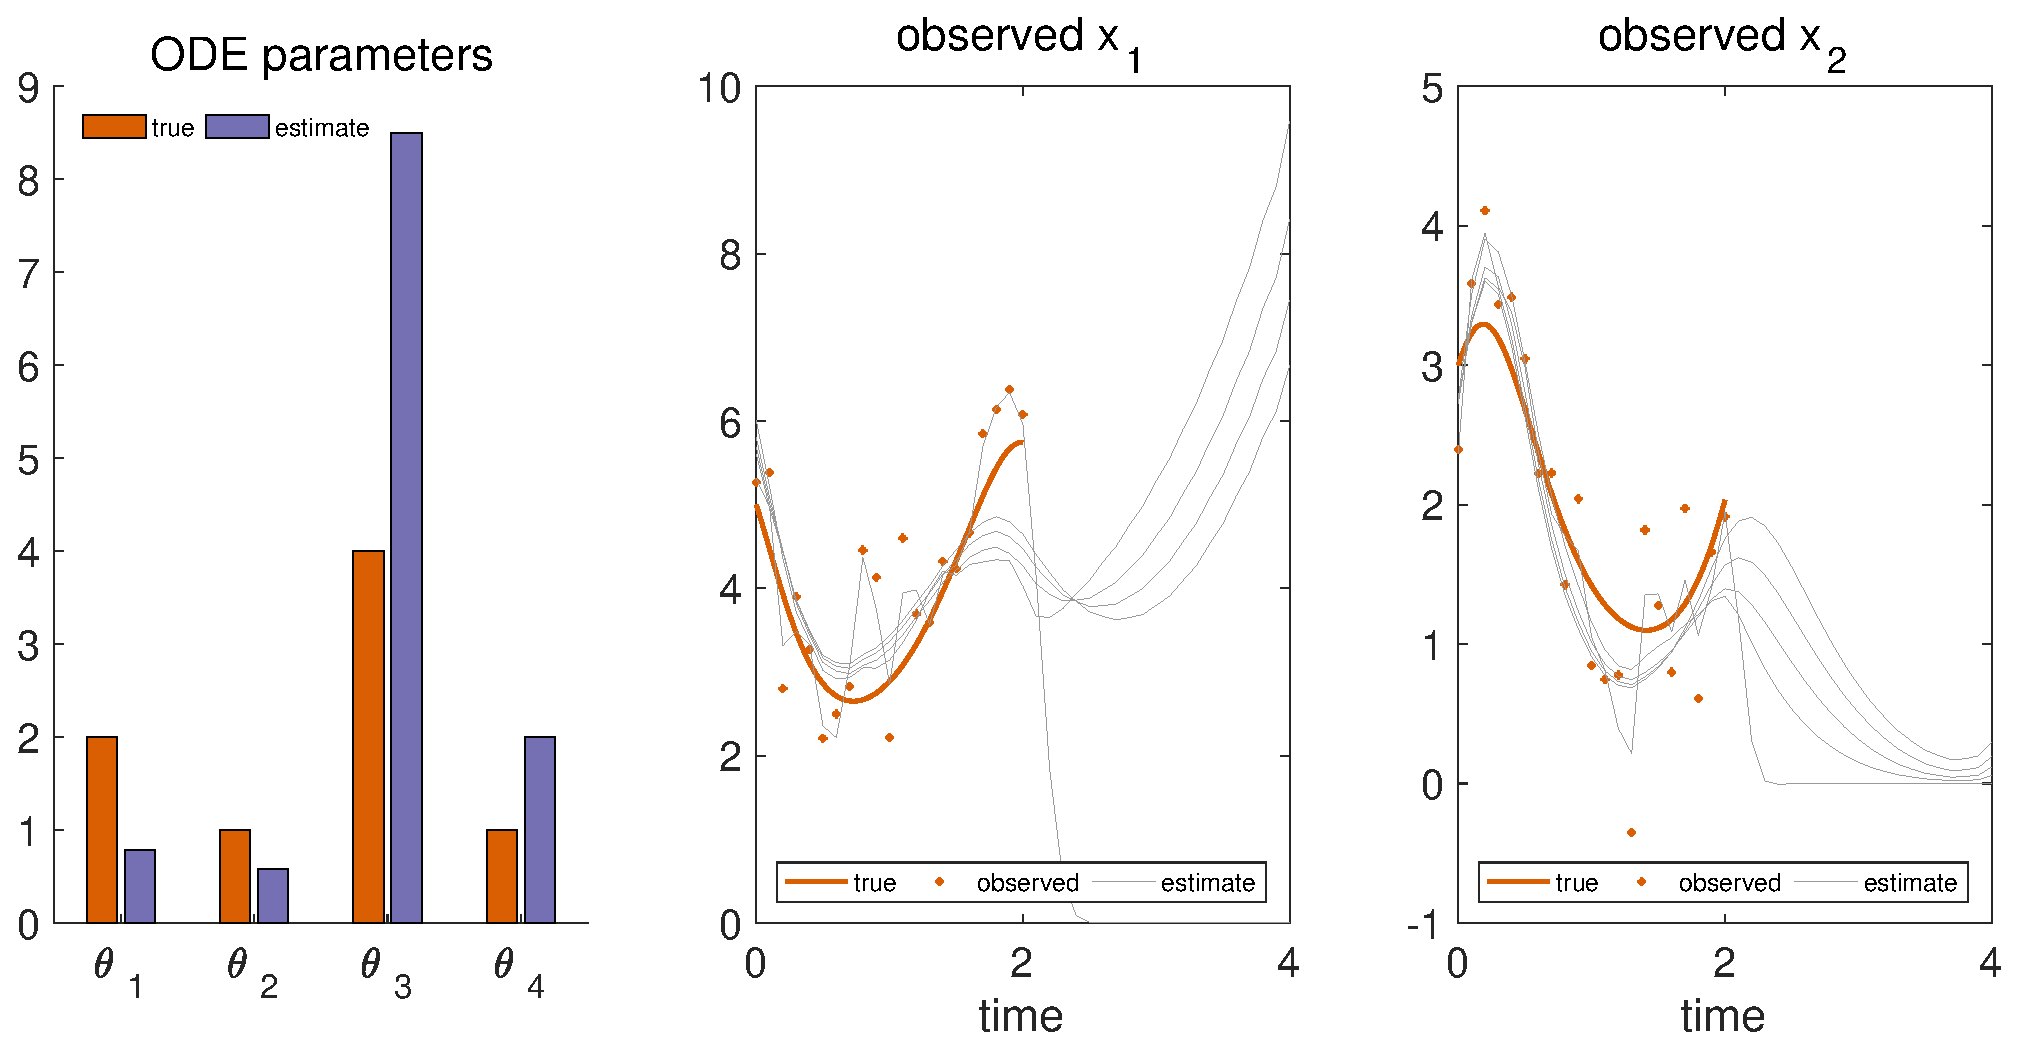
\includegraphics [width=5in]{VGM_for_Lotka_Volterra_06.eps}

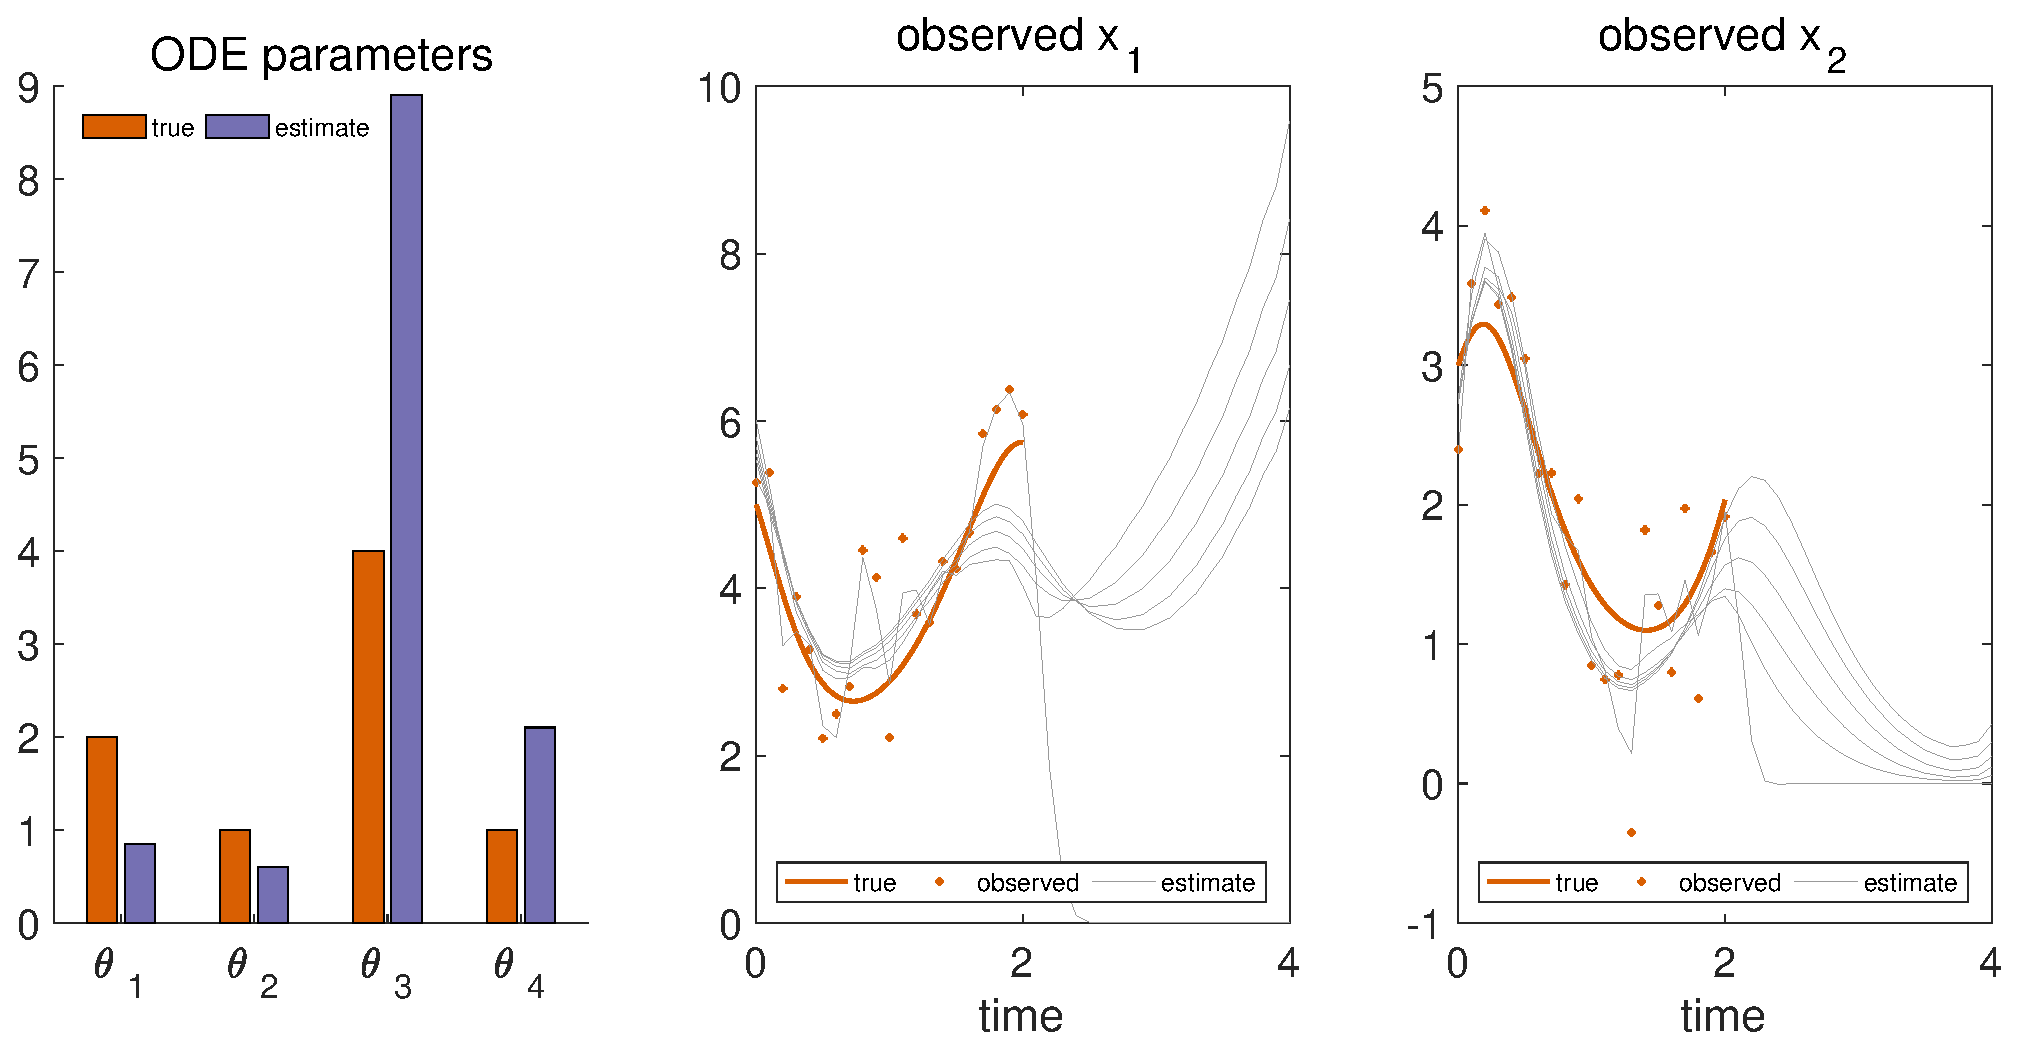
\includegraphics [width=5in]{VGM_for_Lotka_Volterra_07.eps}

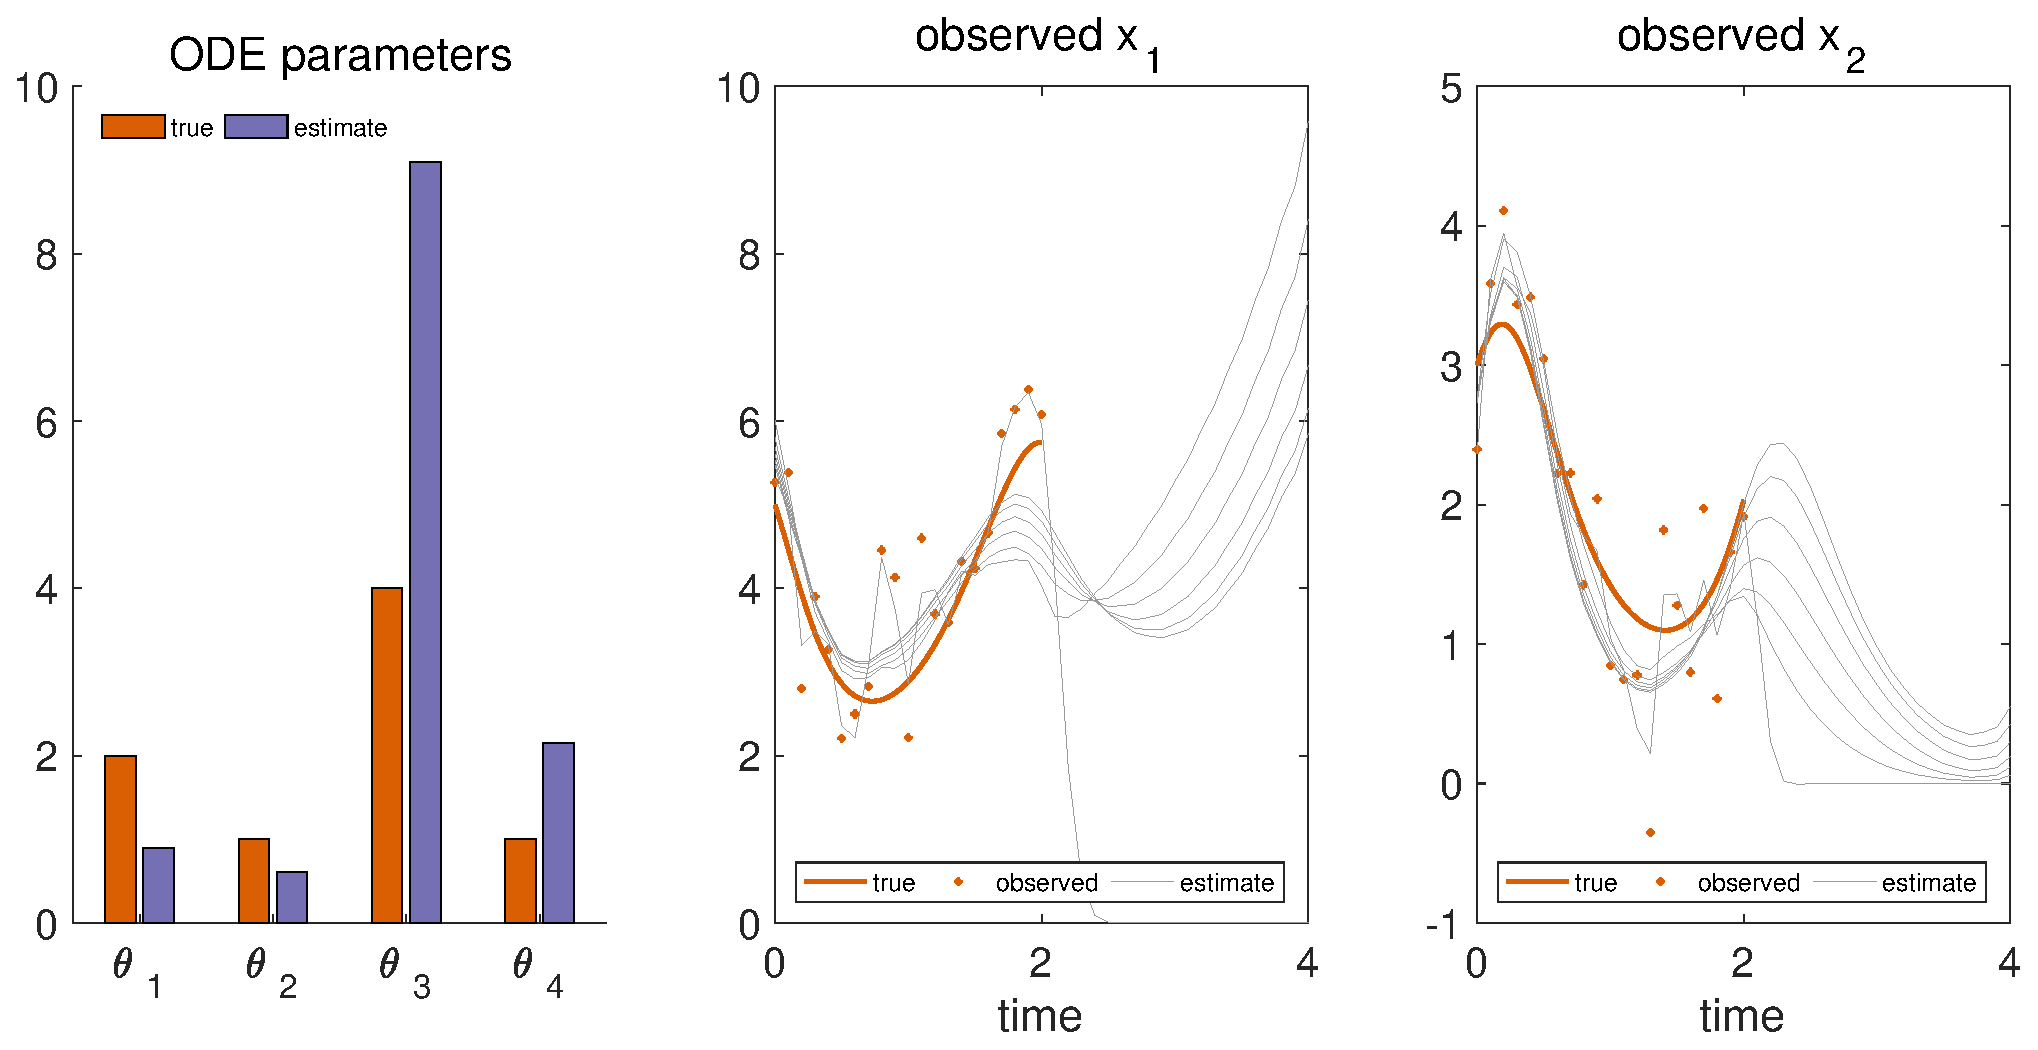
\includegraphics [width=5in]{VGM_for_Lotka_Volterra_08.eps}

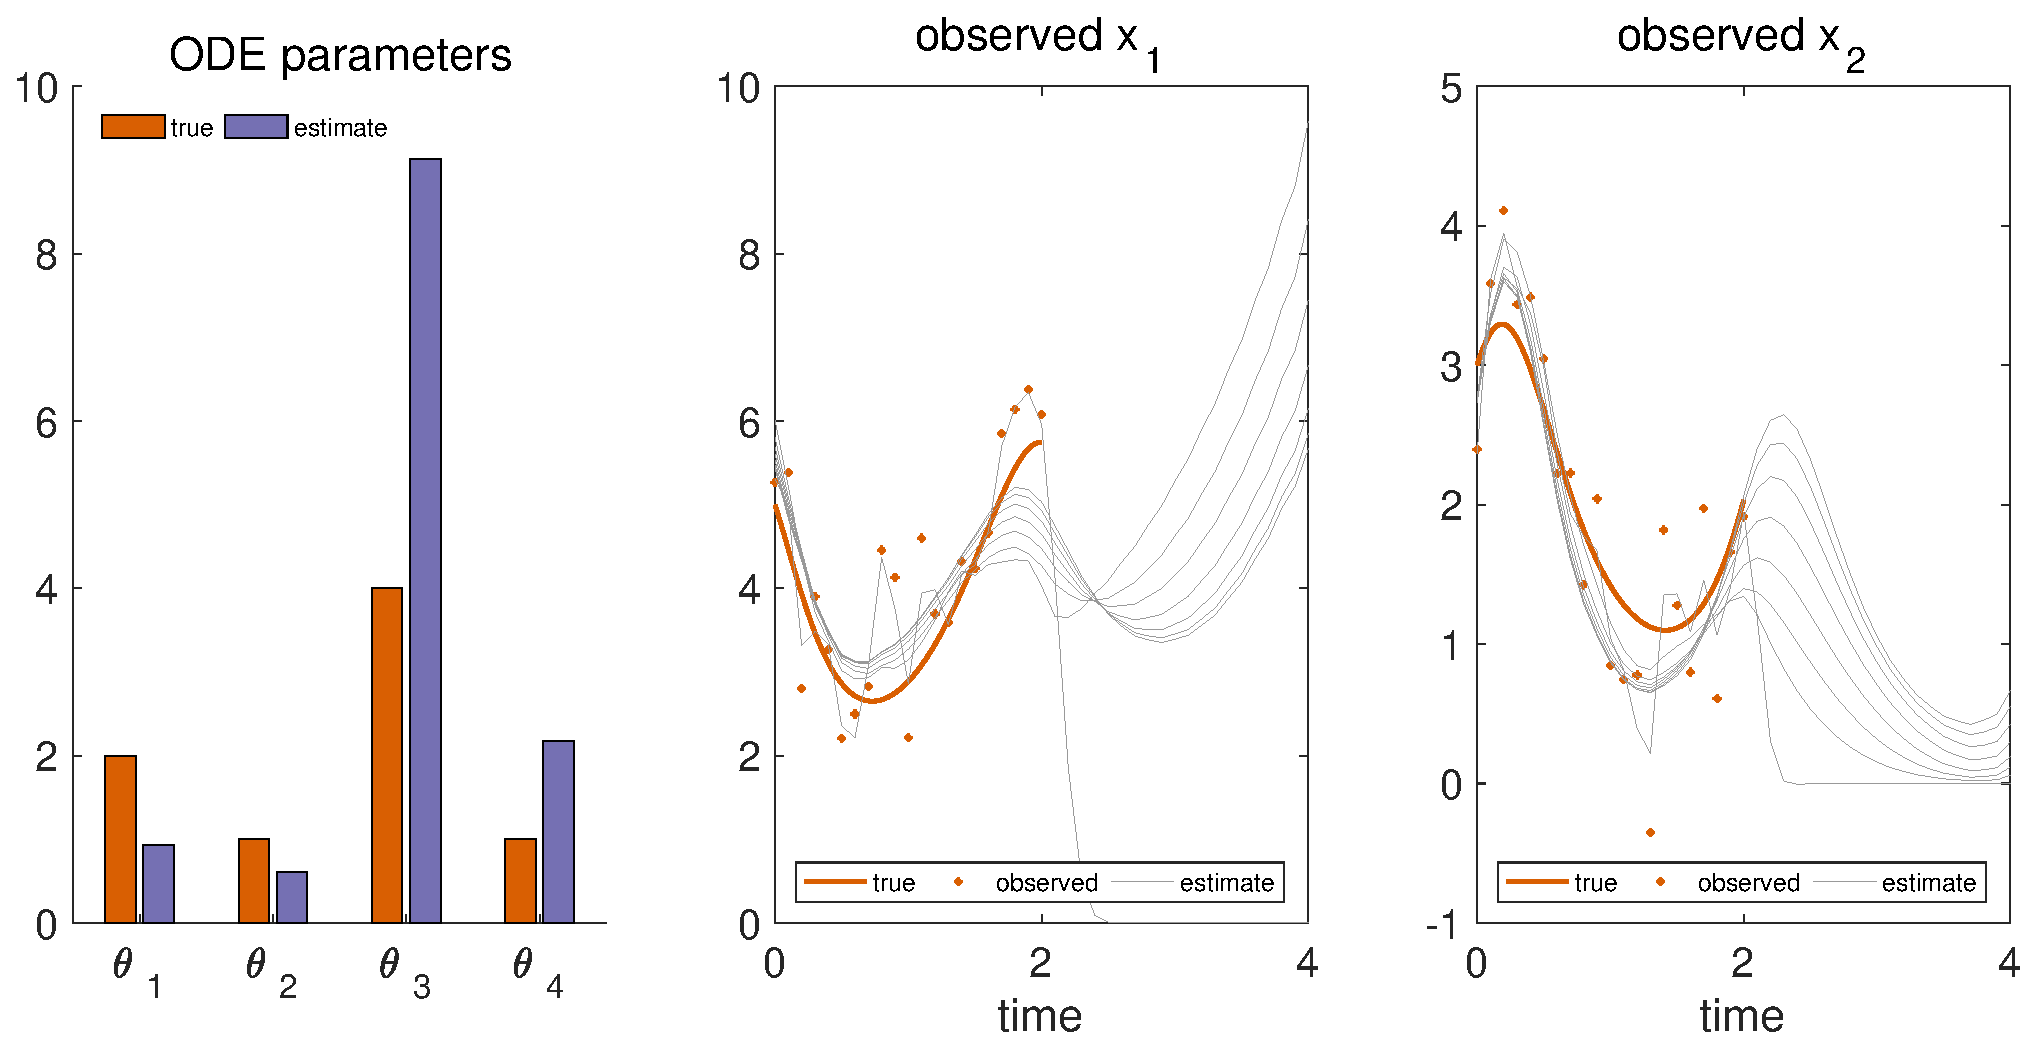
\includegraphics [width=5in]{VGM_for_Lotka_Volterra_09.eps}

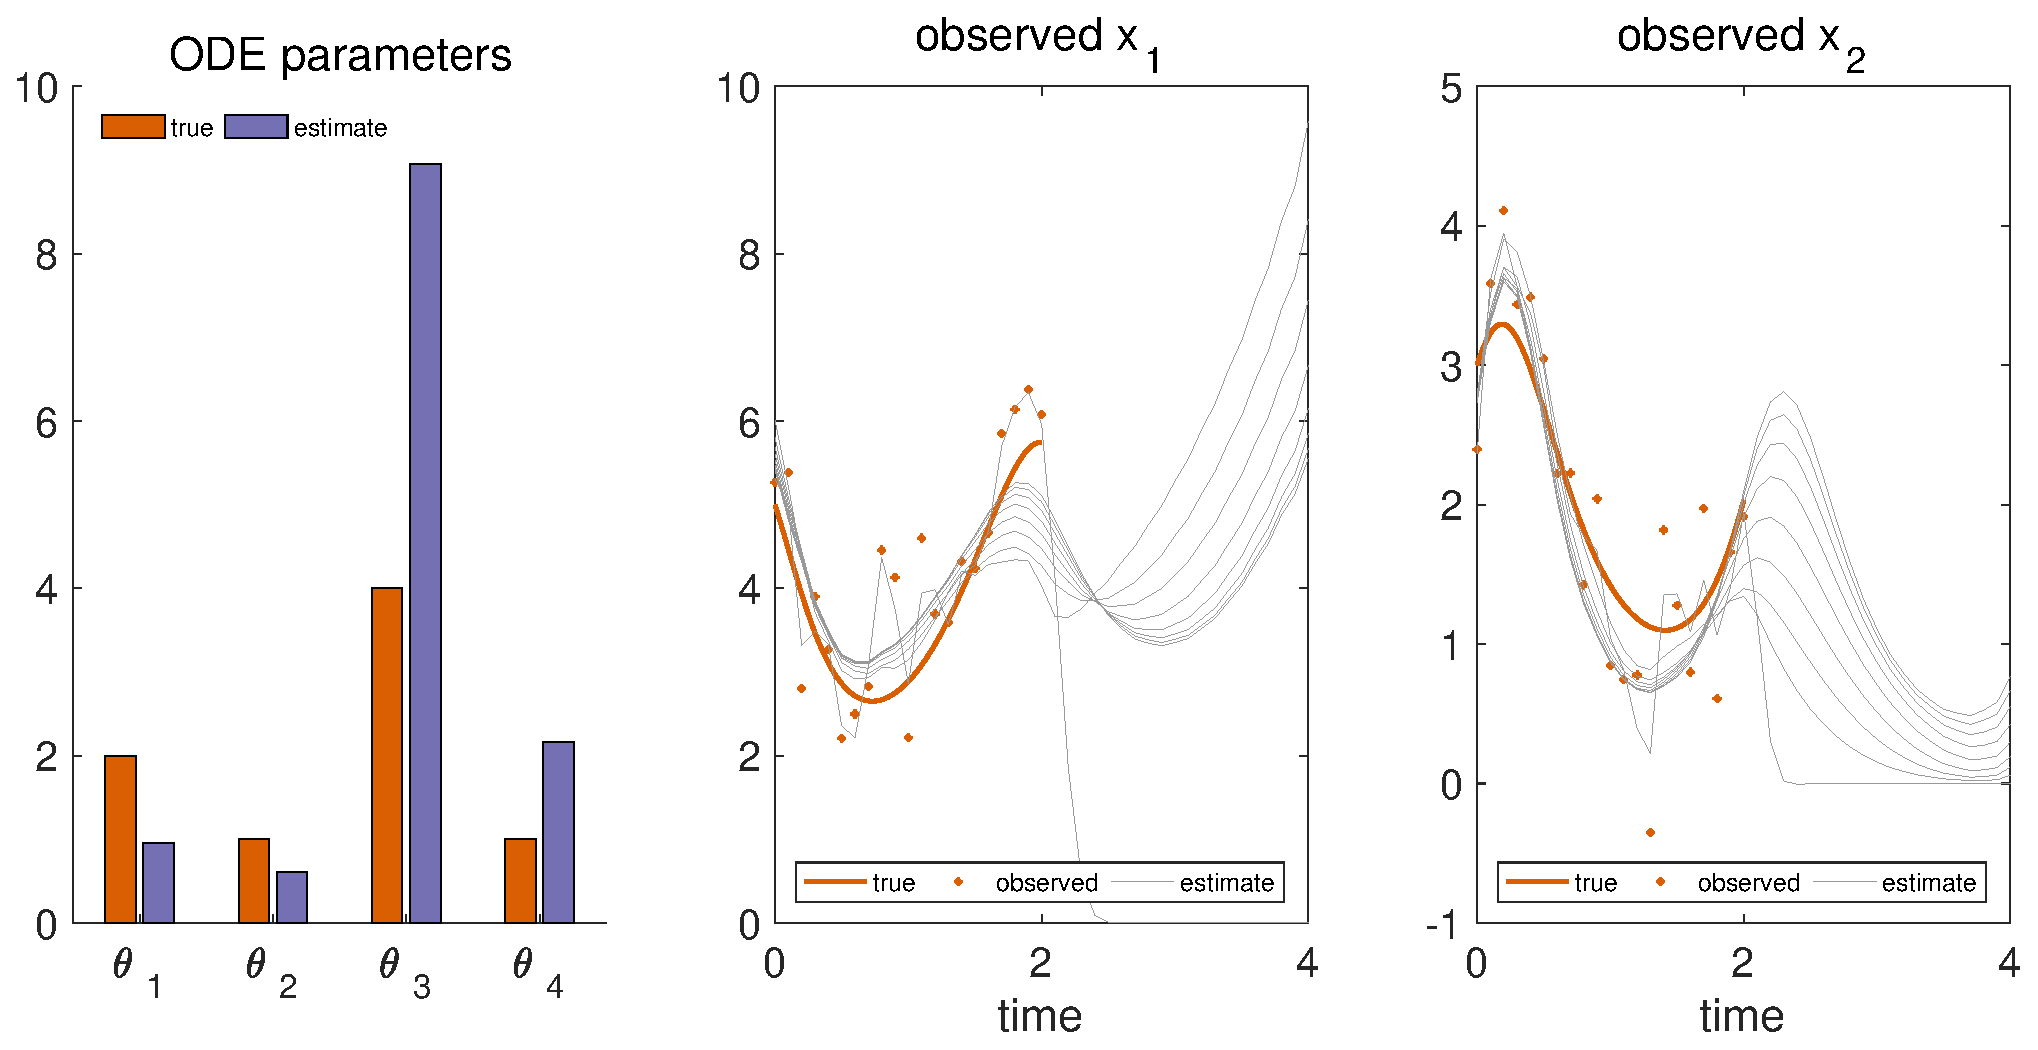
\includegraphics [width=5in]{VGM_for_Lotka_Volterra_10.eps}

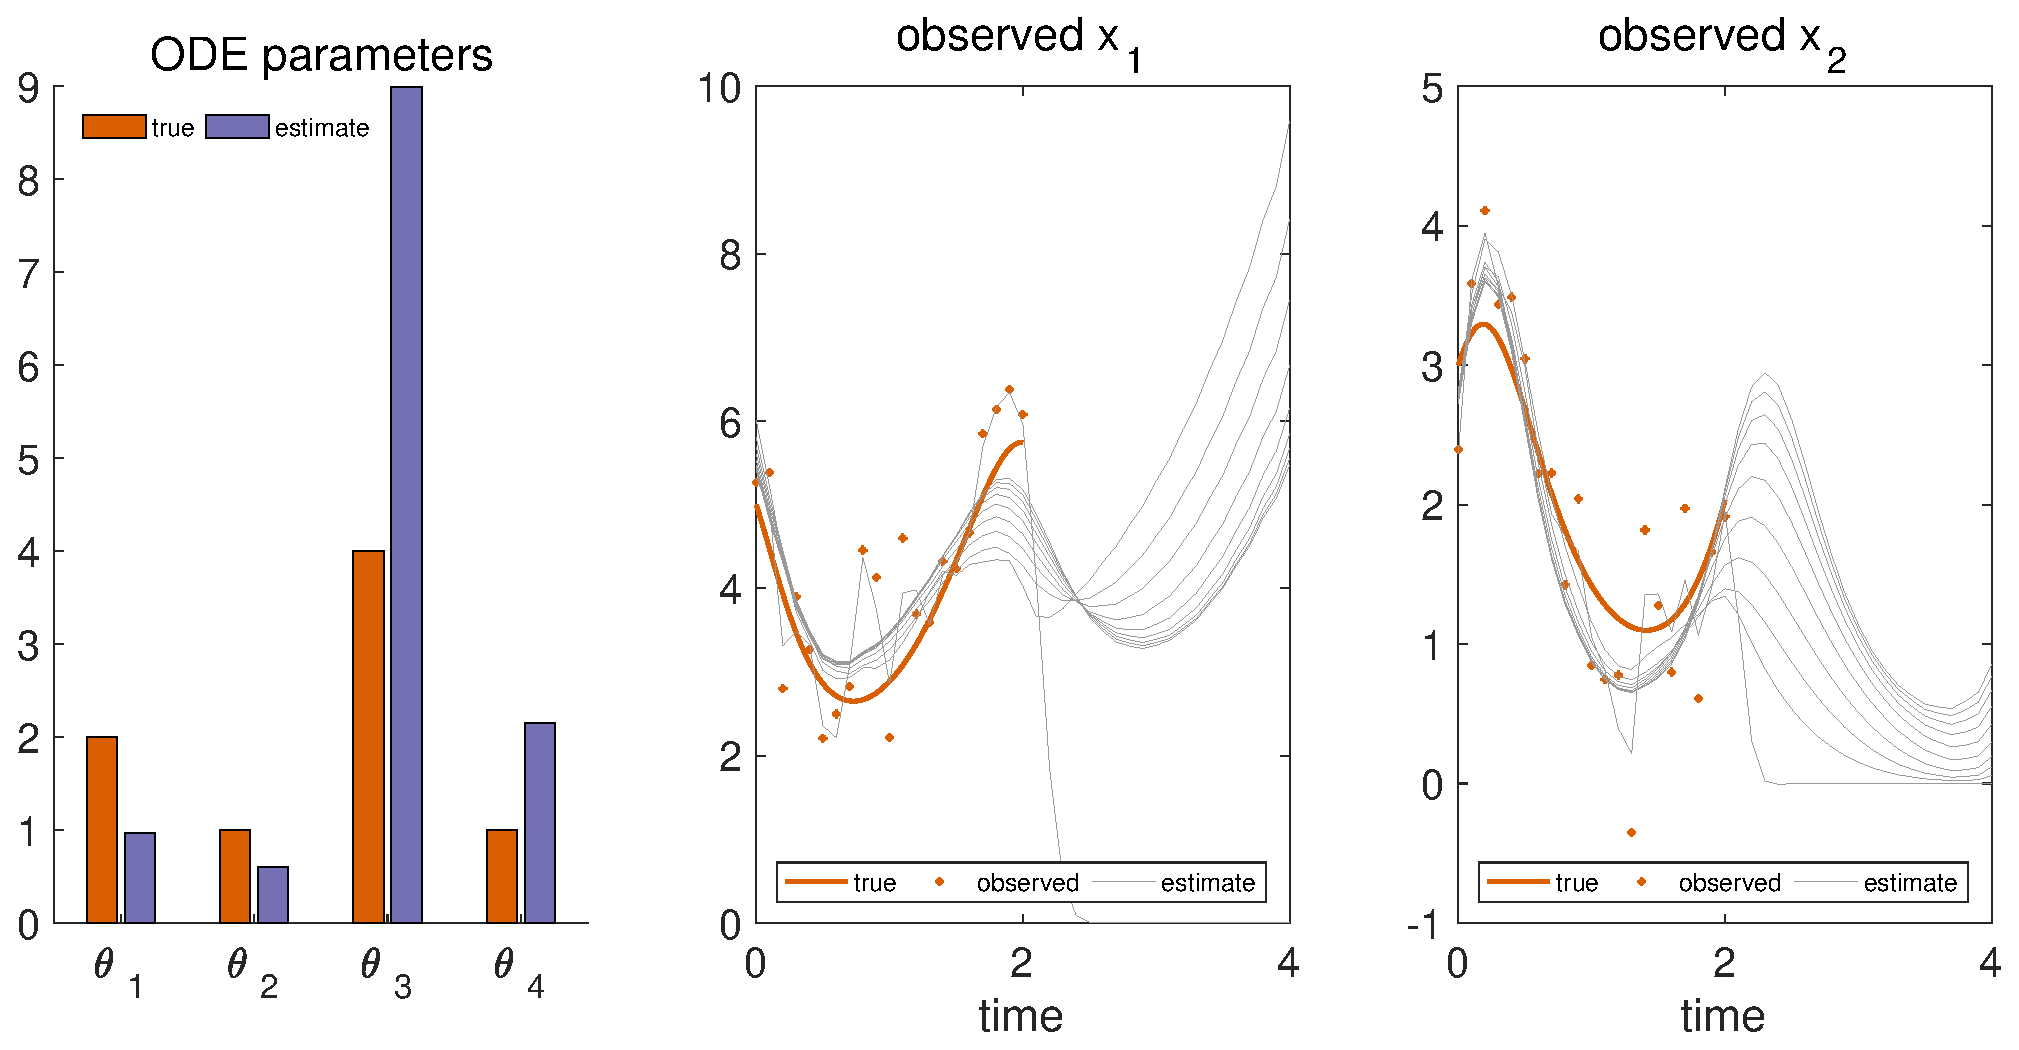
\includegraphics [width=5in]{VGM_for_Lotka_Volterra_11.eps}

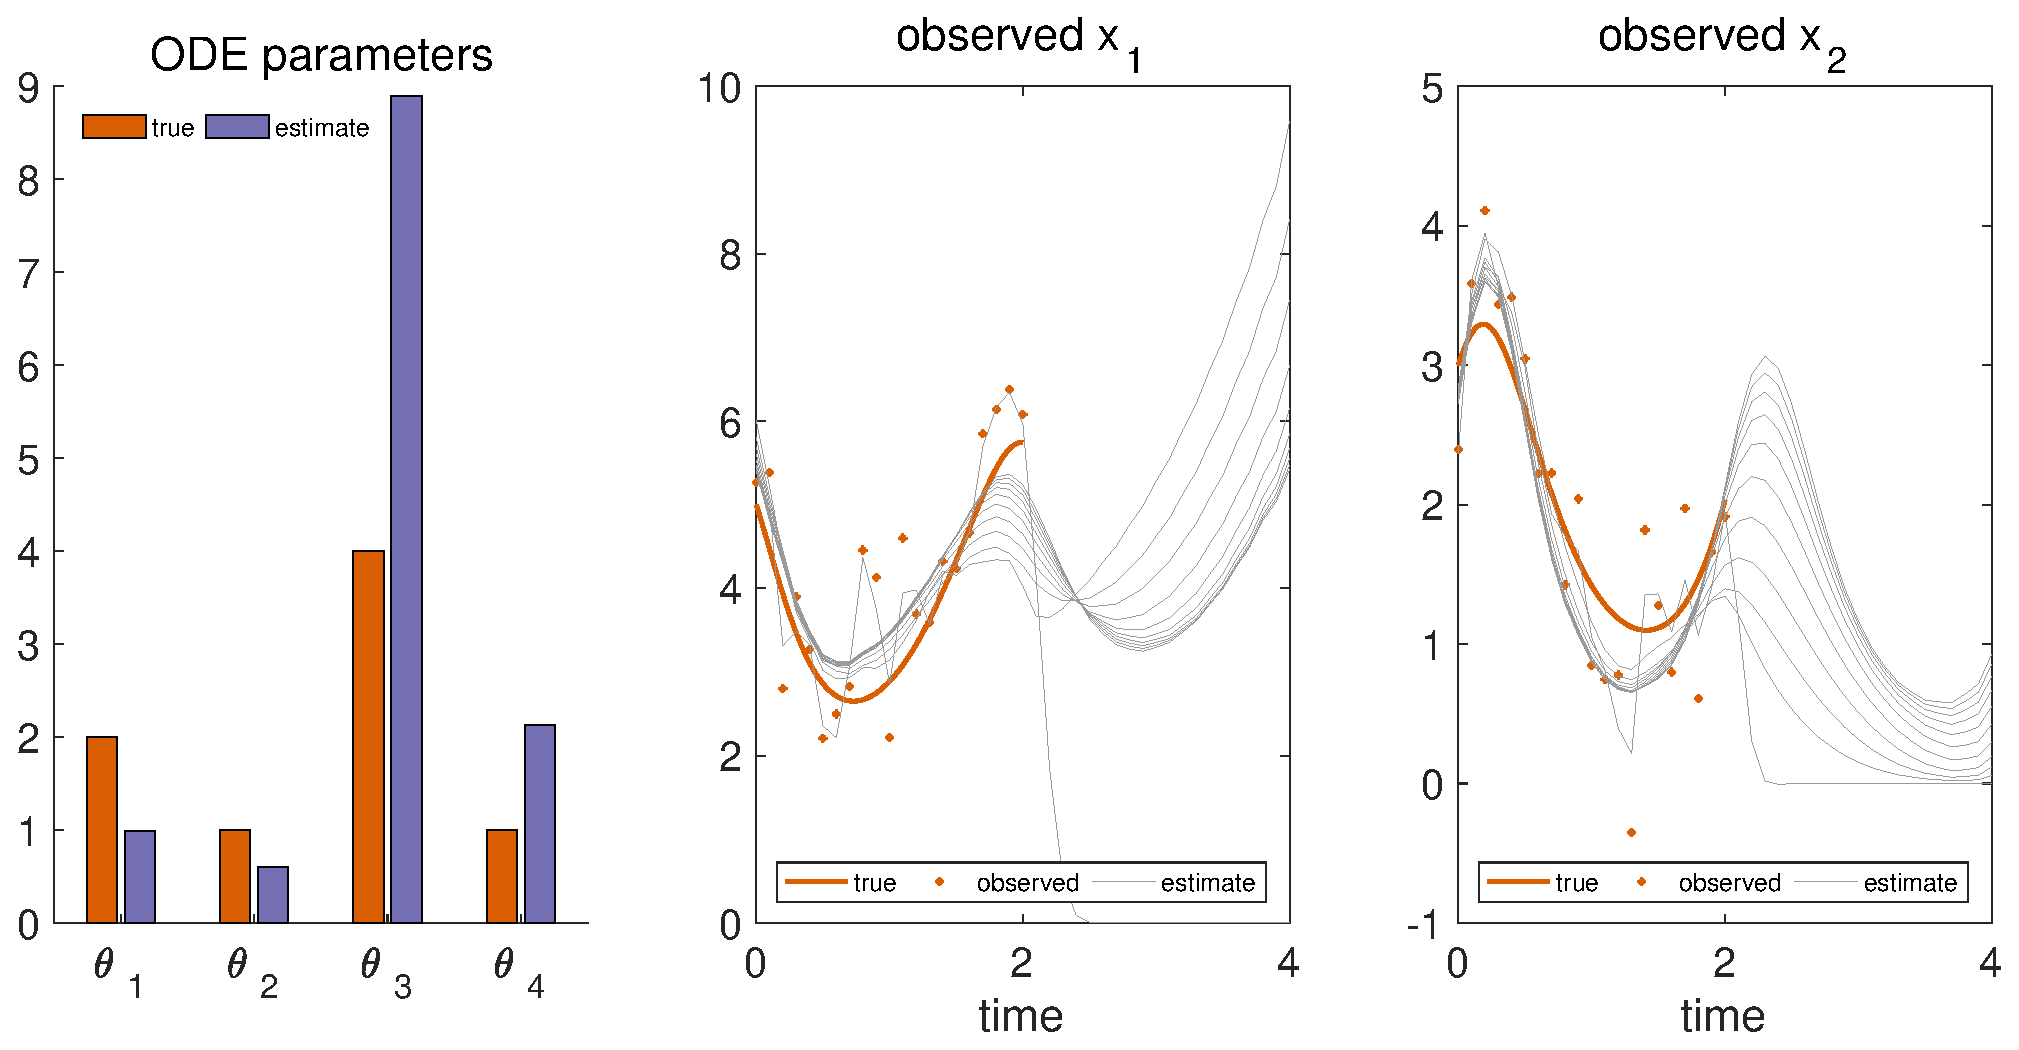
\includegraphics [width=5in]{VGM_for_Lotka_Volterra_12.eps}

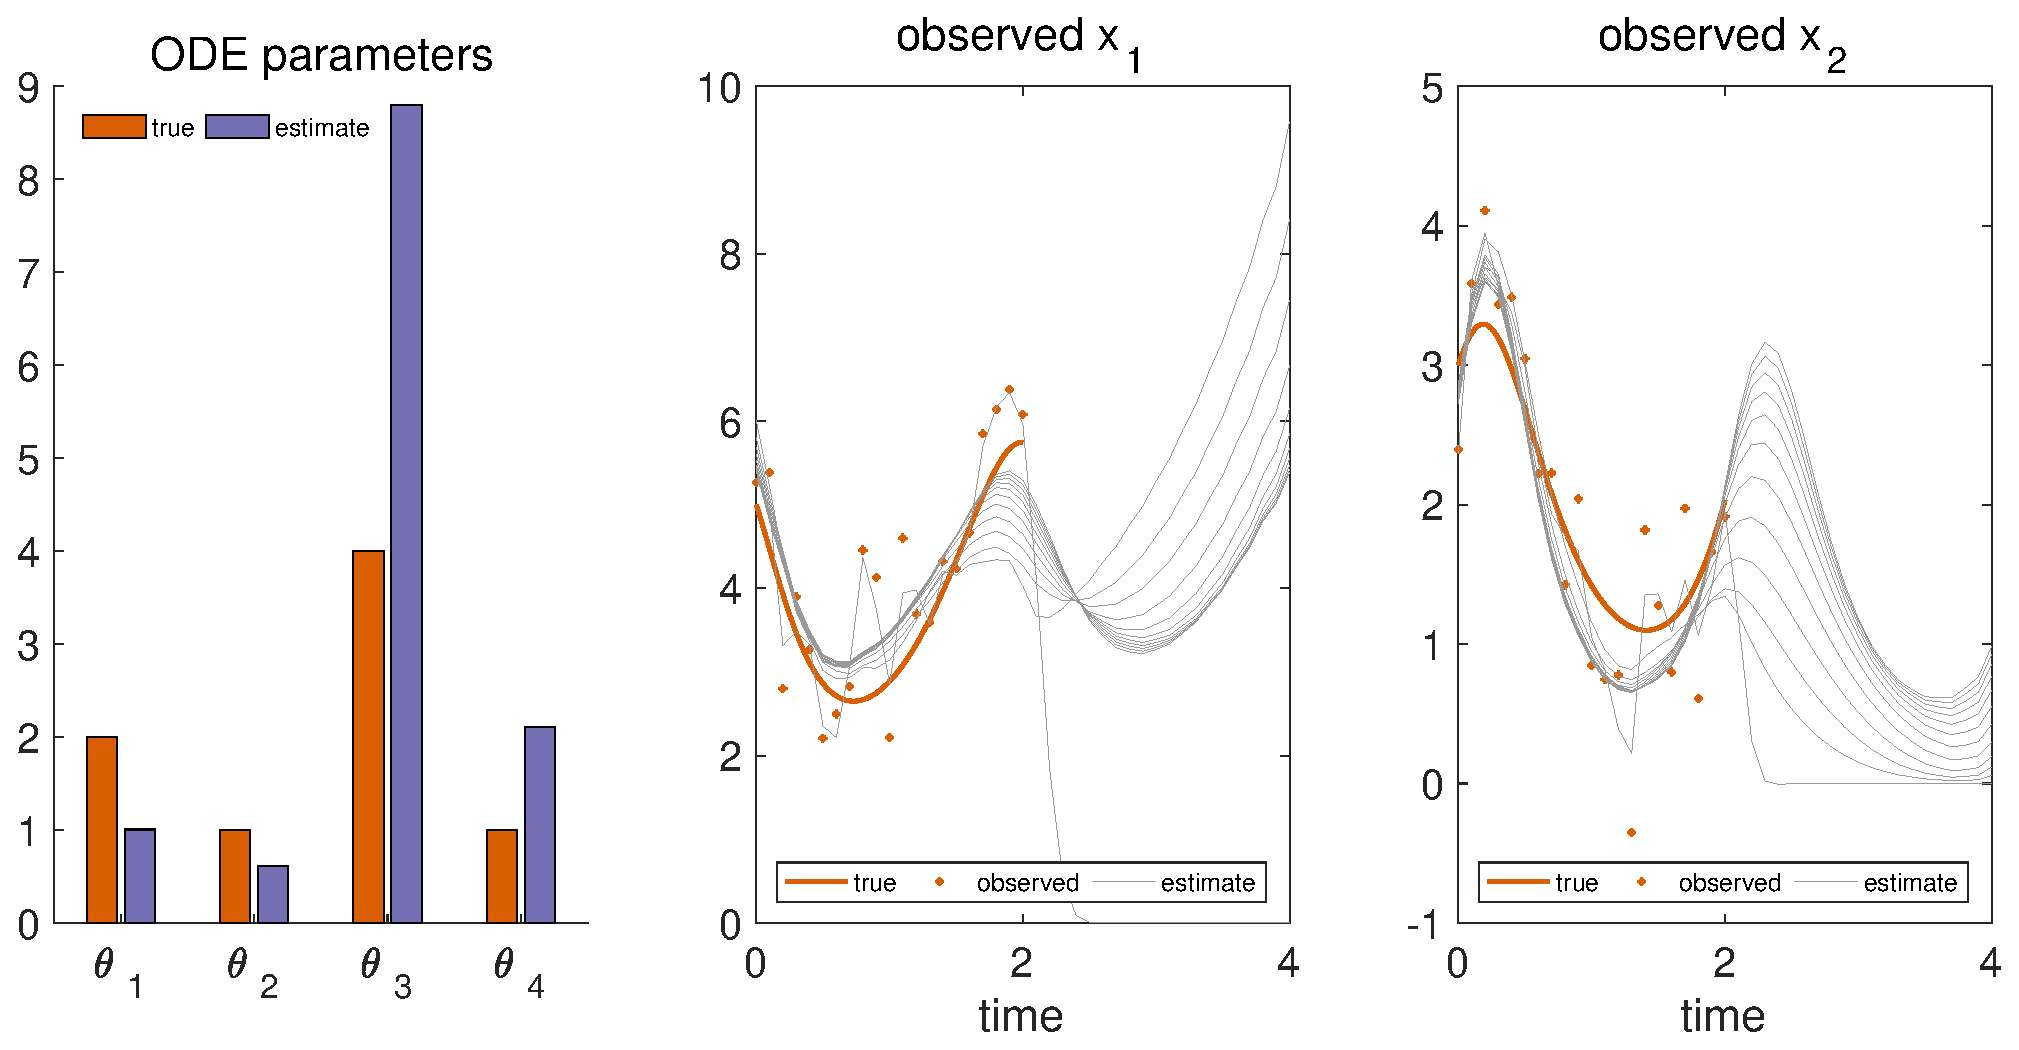
\includegraphics [width=5in]{VGM_for_Lotka_Volterra_13.eps}

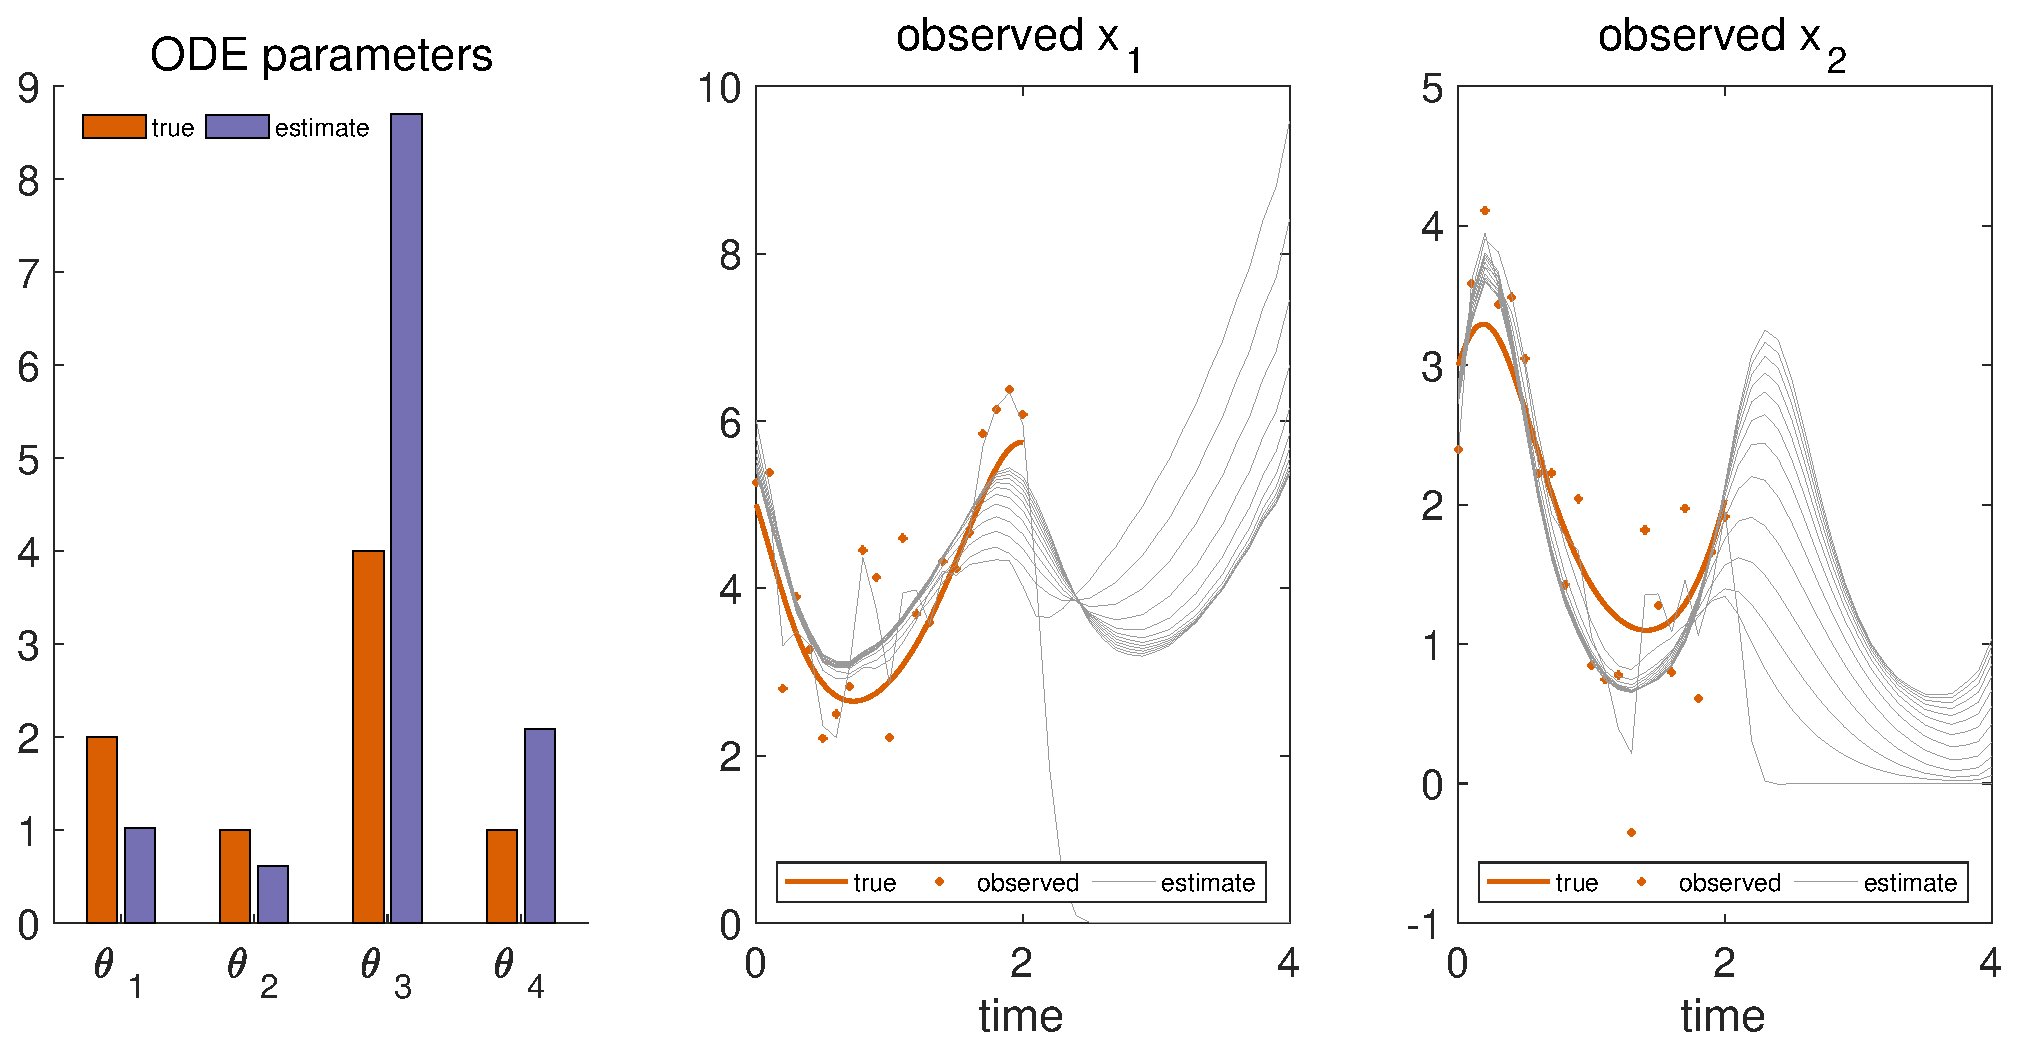
\includegraphics [width=5in]{VGM_for_Lotka_Volterra_14.eps}

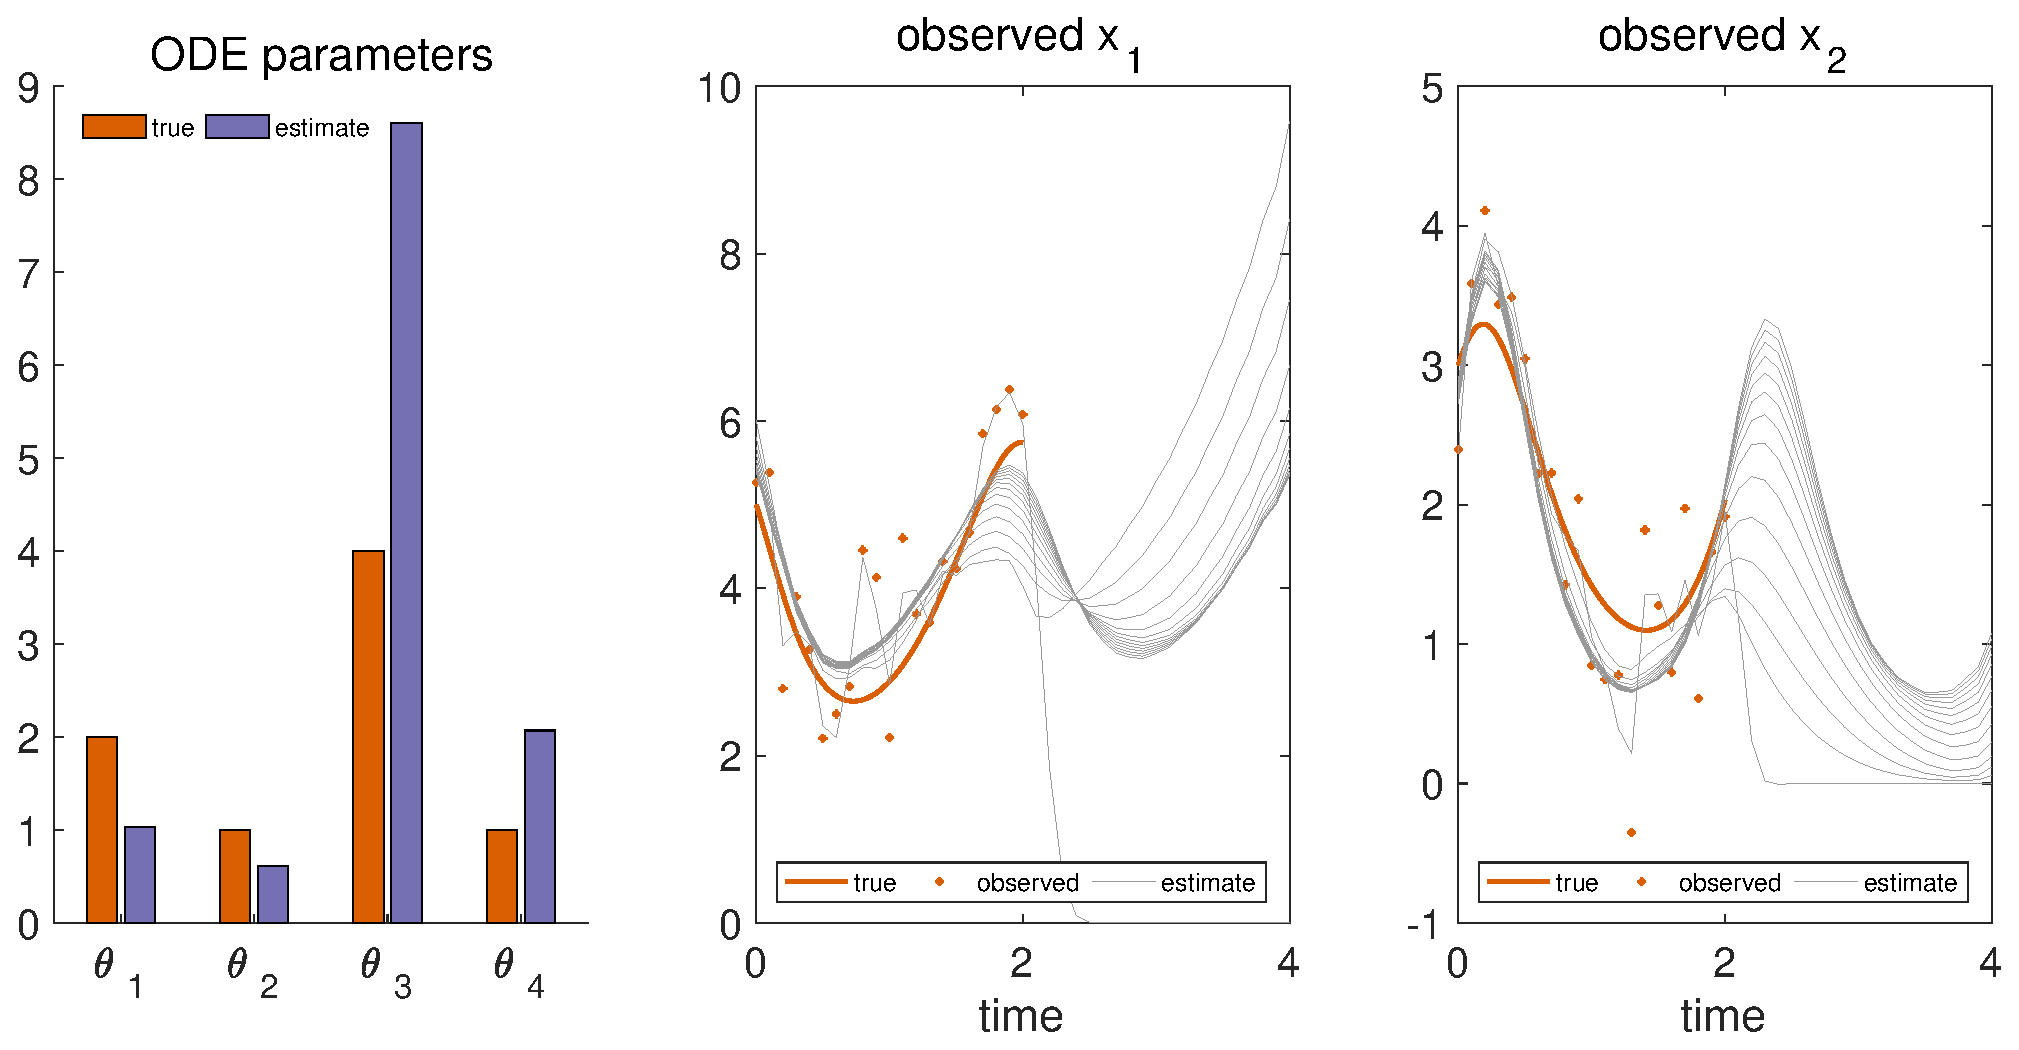
\includegraphics [width=5in]{VGM_for_Lotka_Volterra_15.eps}

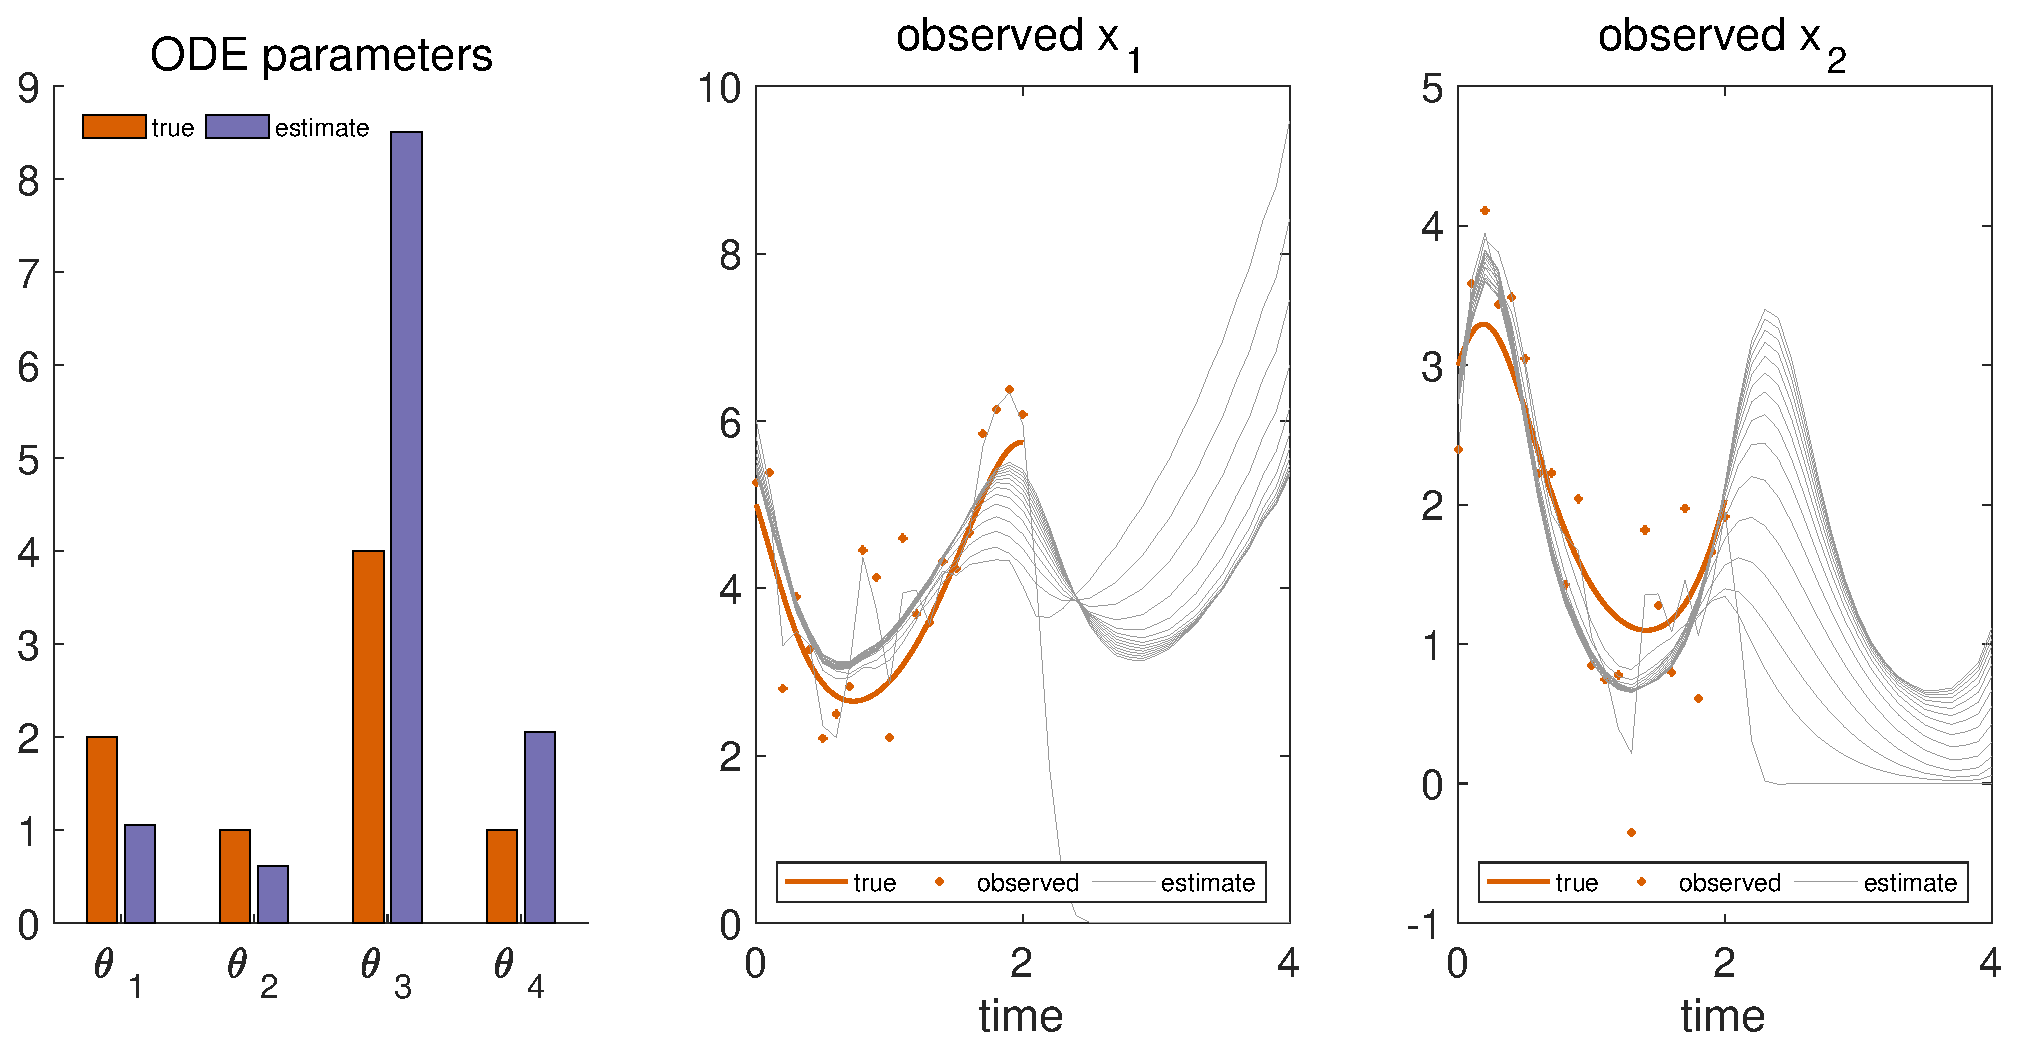
\includegraphics [width=5in]{VGM_for_Lotka_Volterra_16.eps}

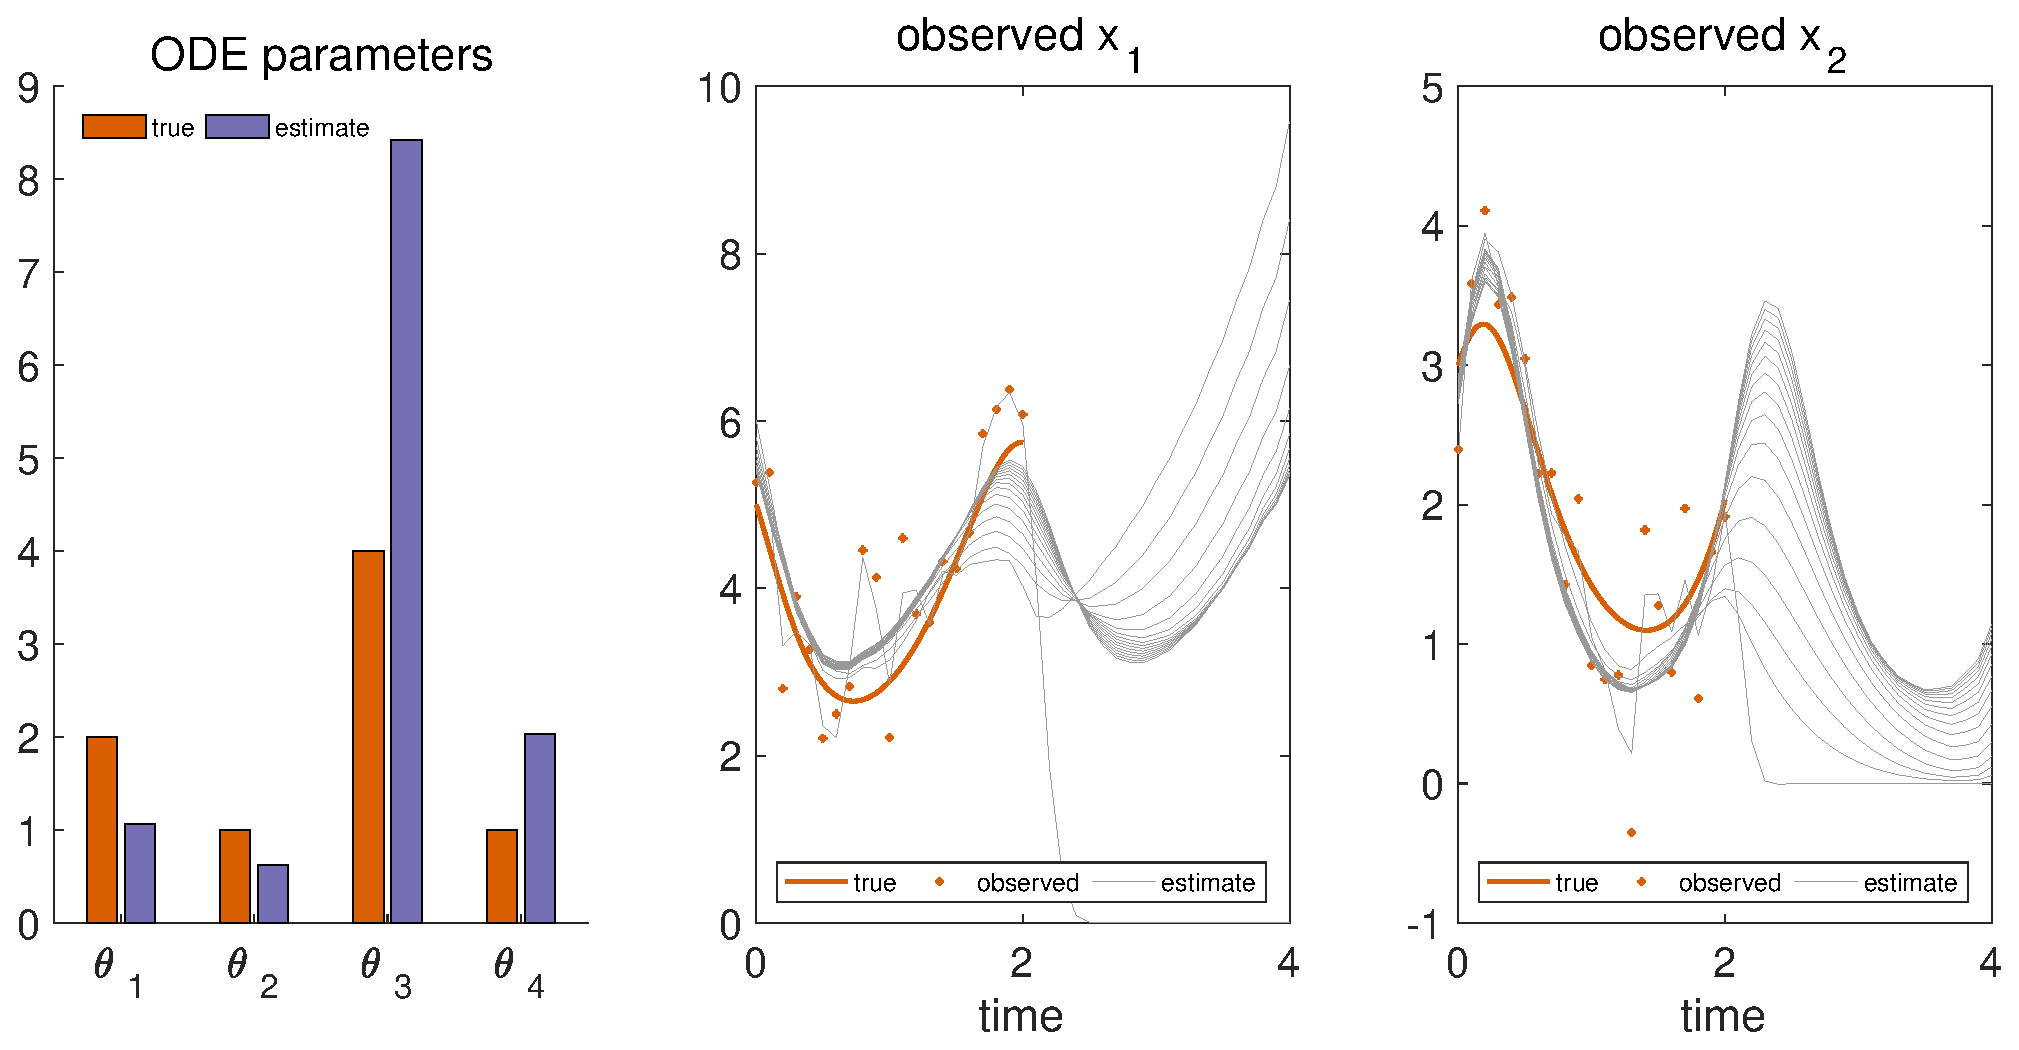
\includegraphics [width=5in]{VGM_for_Lotka_Volterra_17.eps}

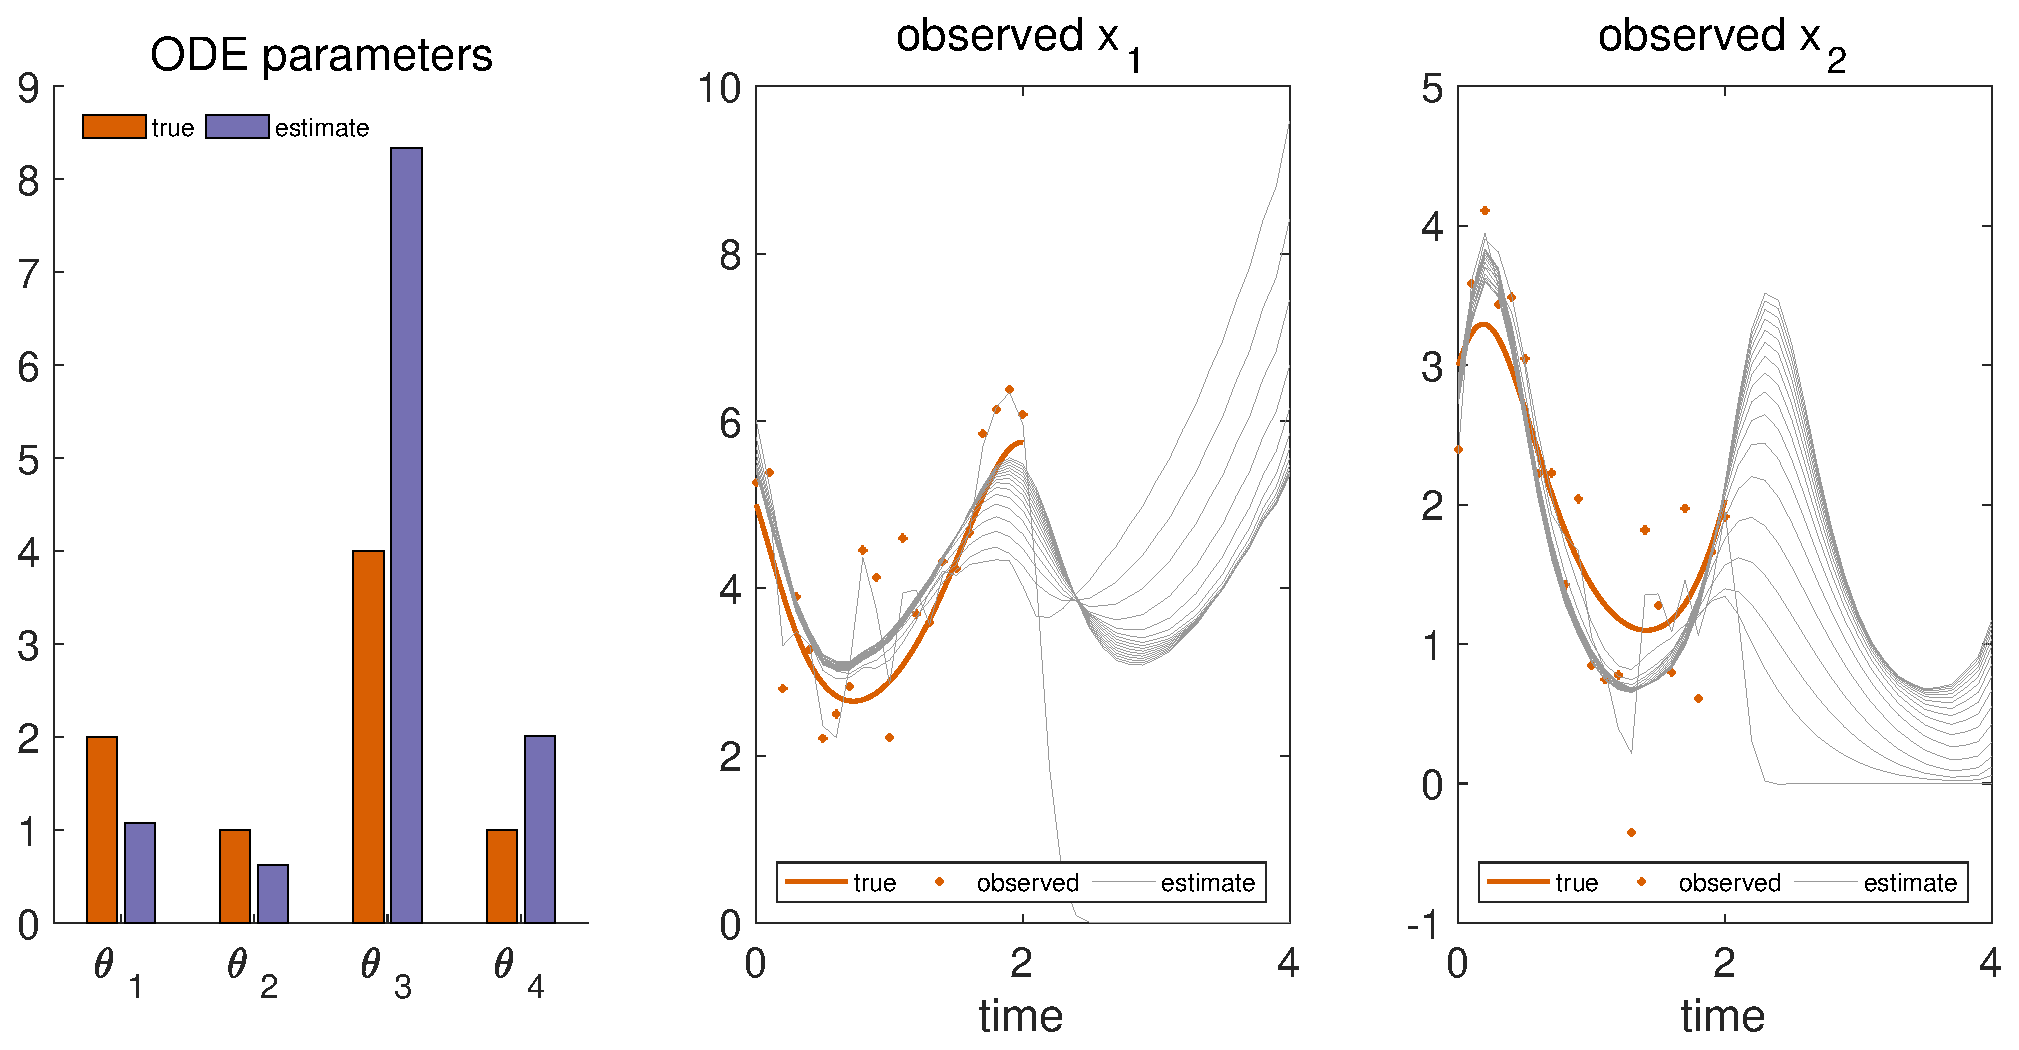
\includegraphics [width=5in]{VGM_for_Lotka_Volterra_18.eps}

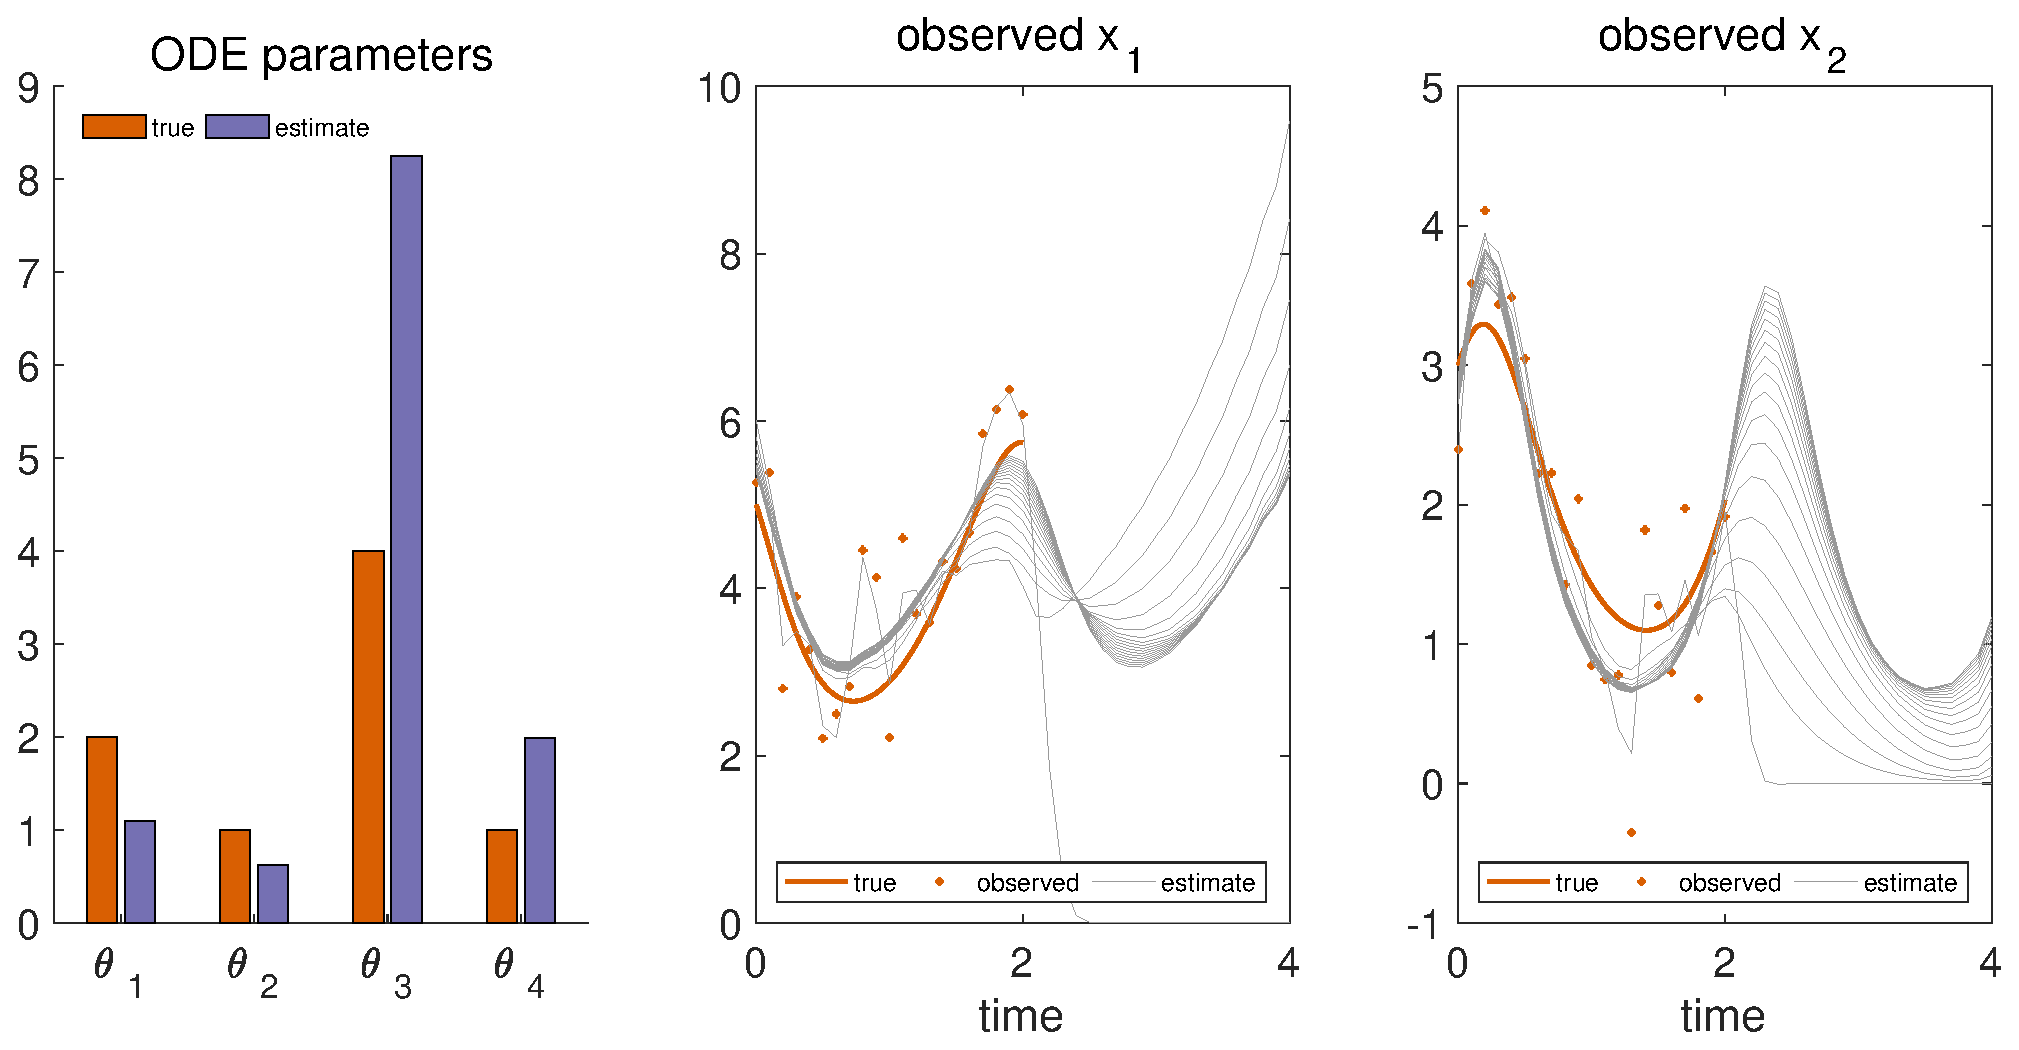
\includegraphics [width=5in]{VGM_for_Lotka_Volterra_19.eps}

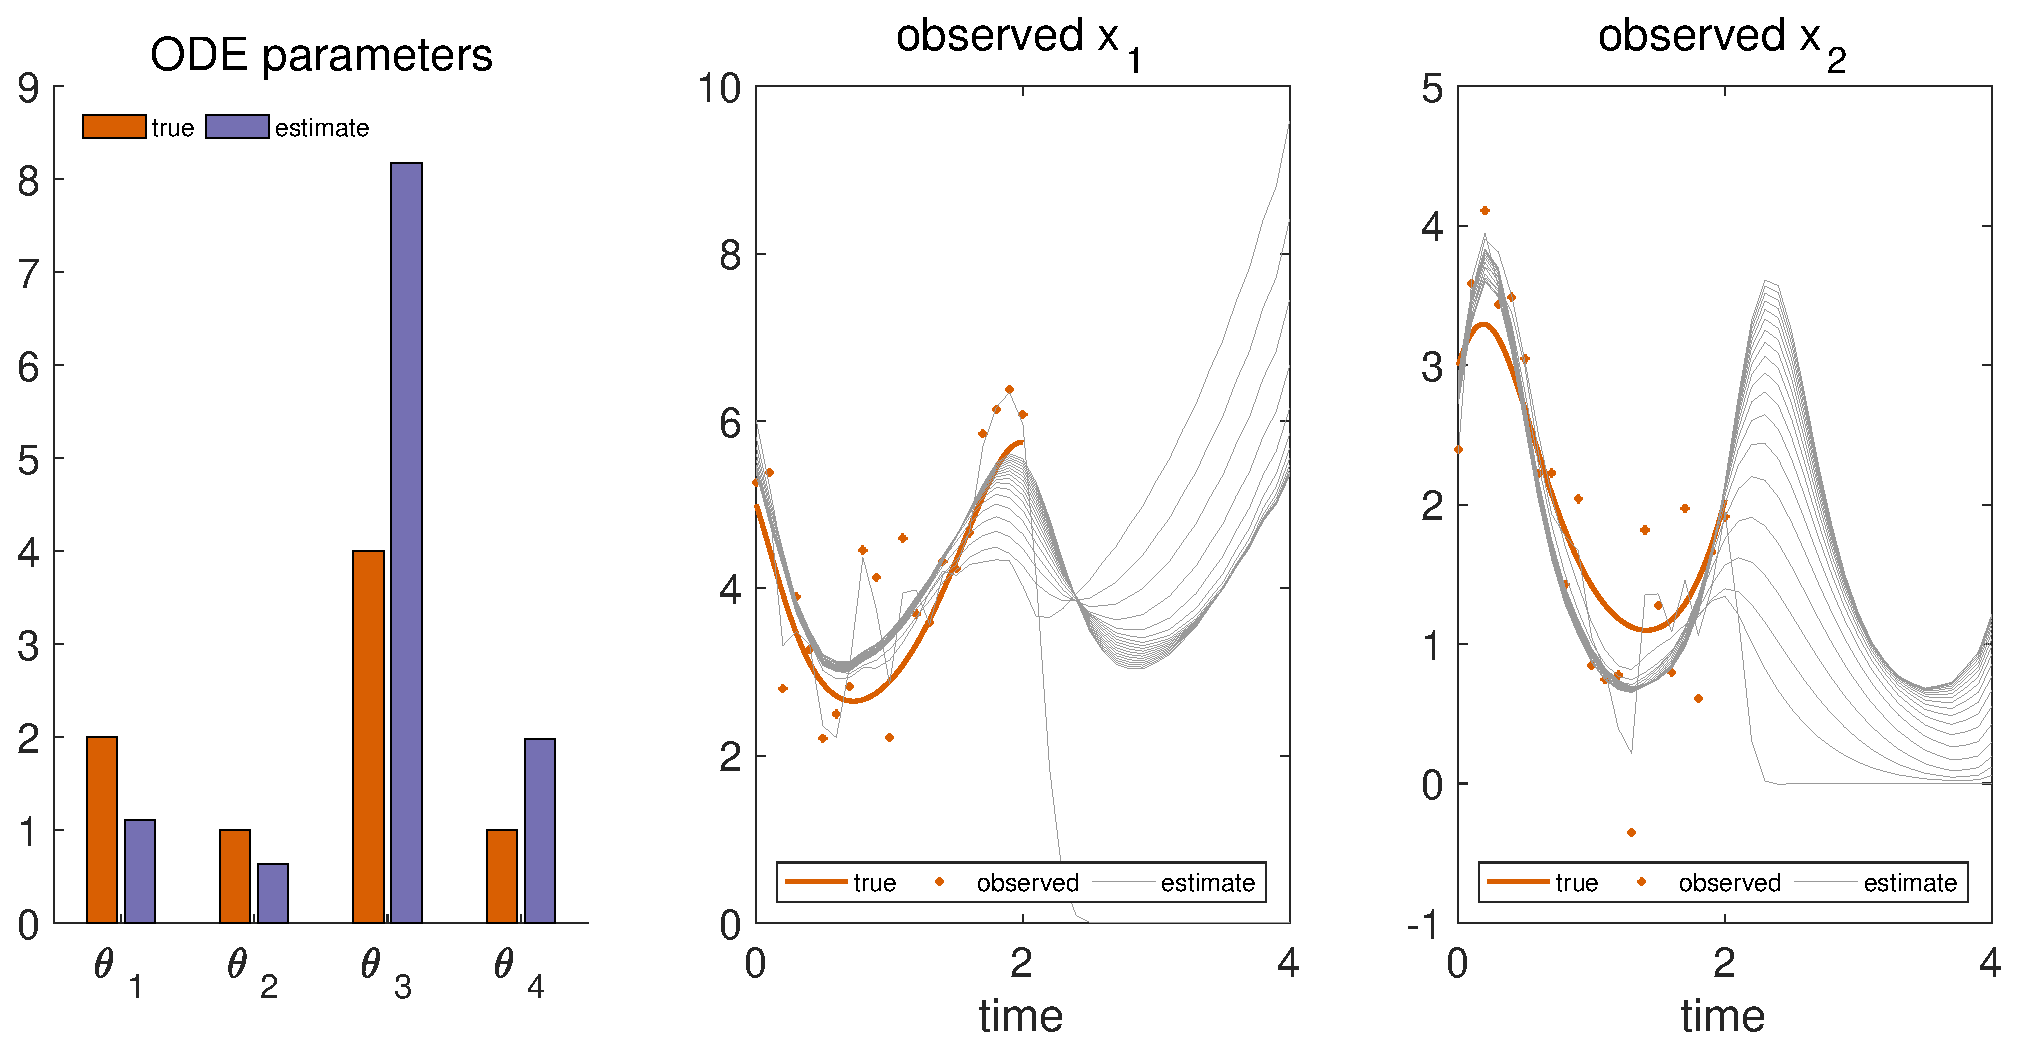
\includegraphics [width=5in]{VGM_for_Lotka_Volterra_20.eps}

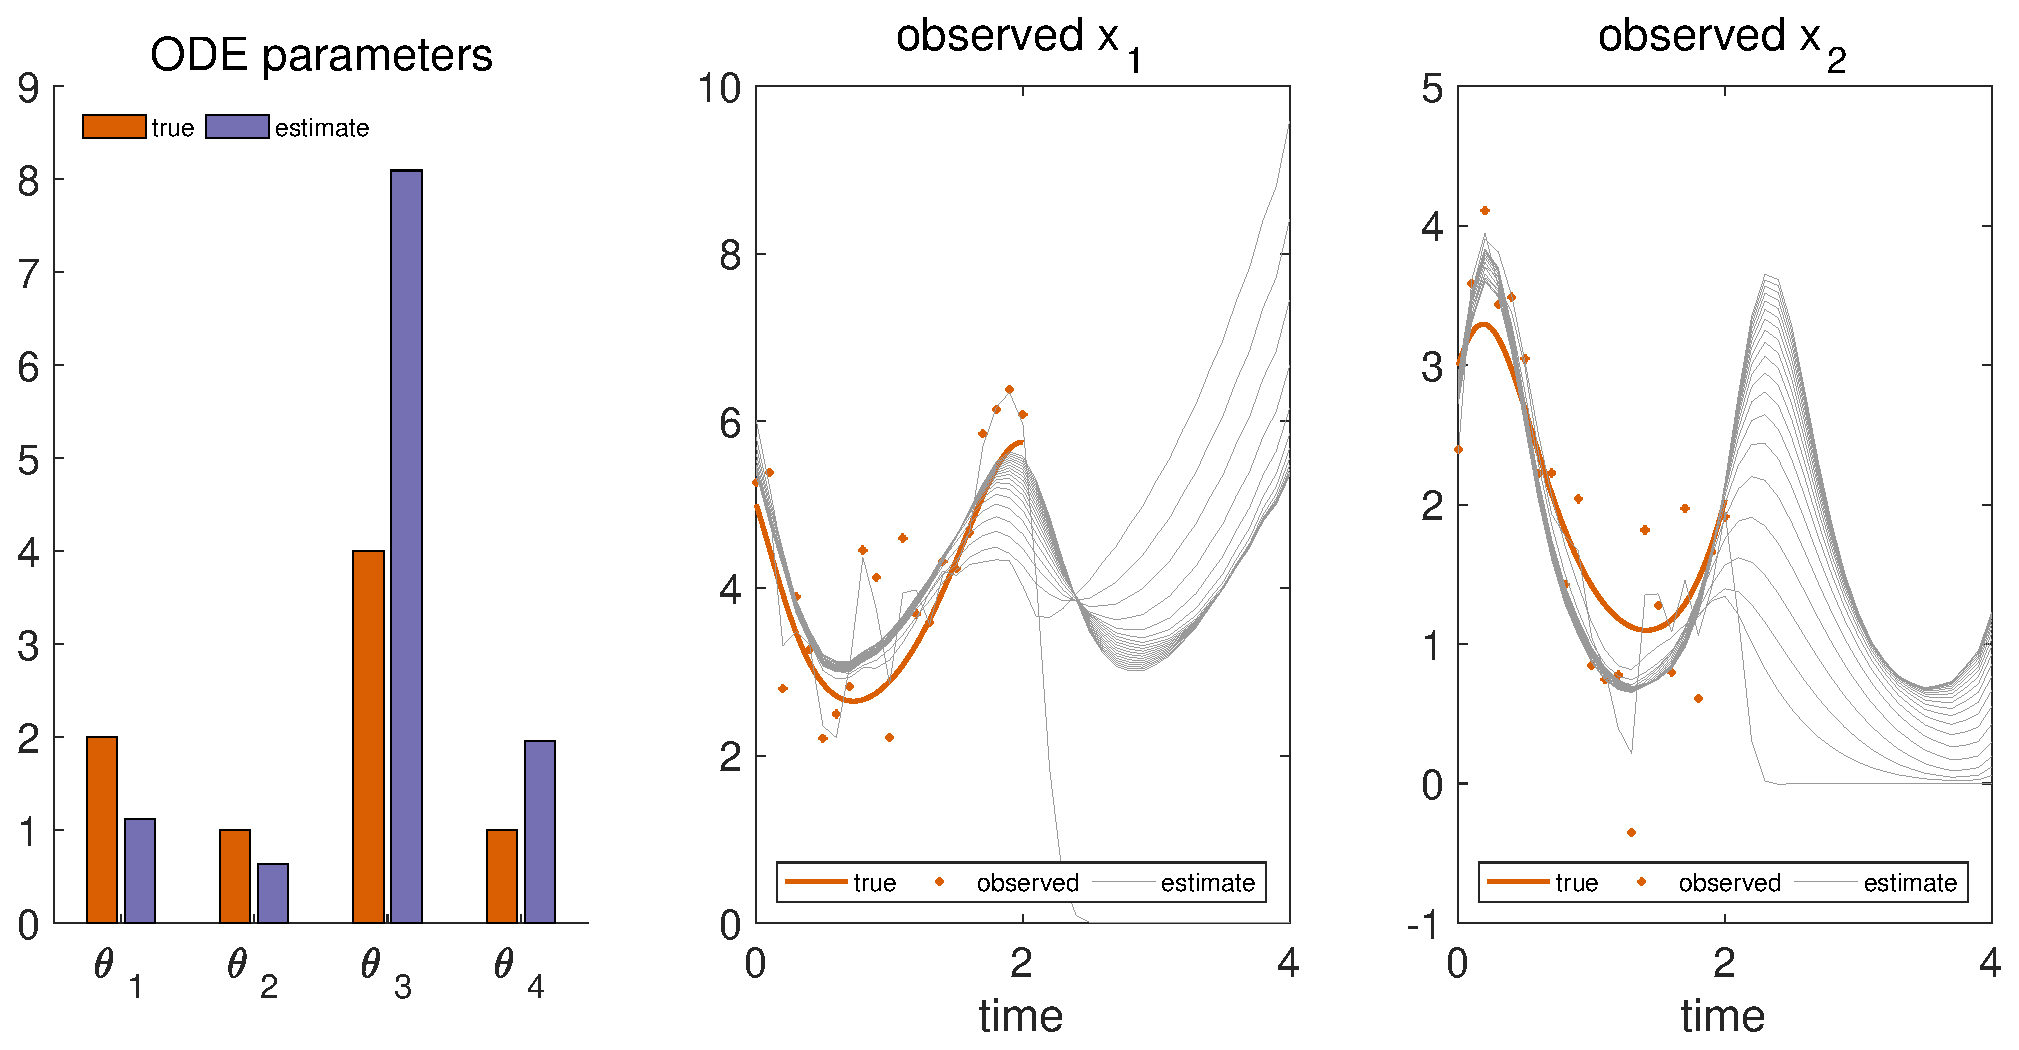
\includegraphics [width=5in]{VGM_for_Lotka_Volterra_21.eps}

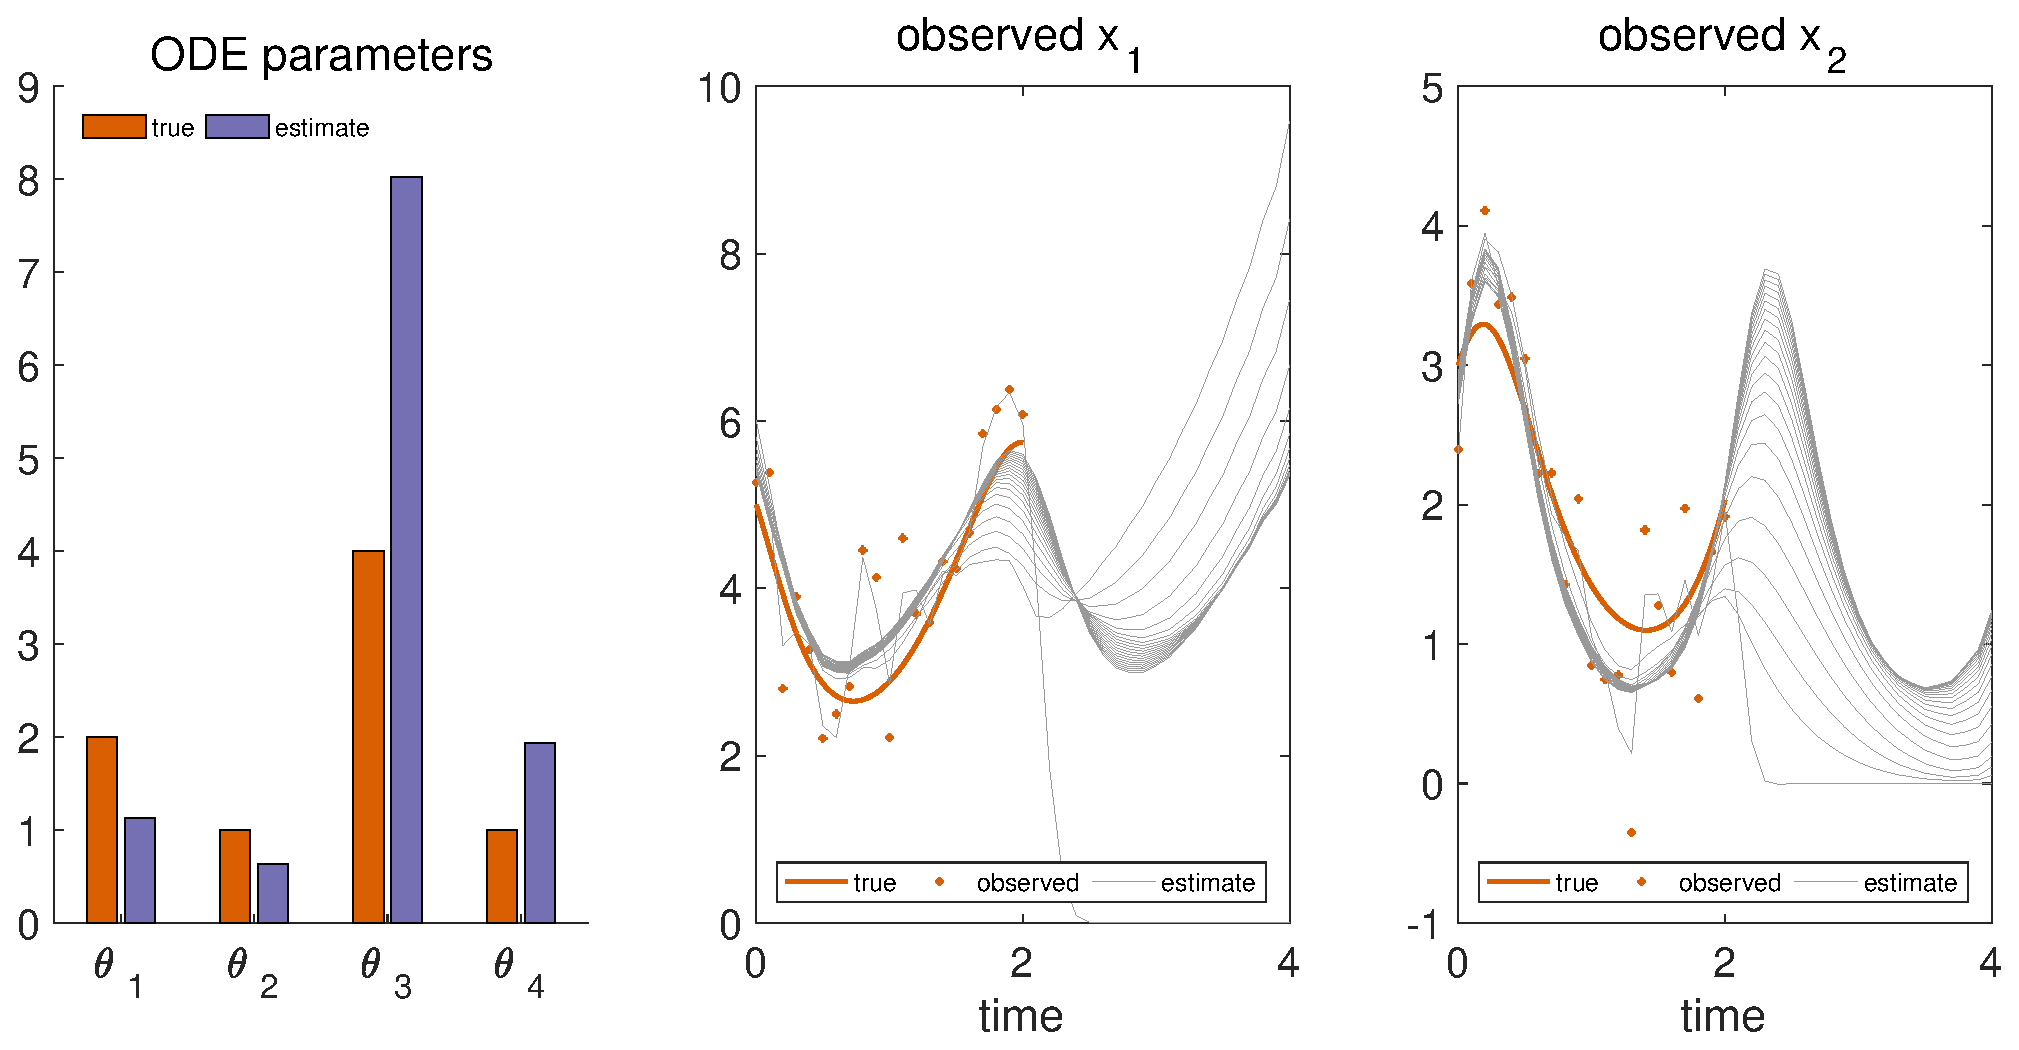
\includegraphics [width=5in]{VGM_for_Lotka_Volterra_22.eps}

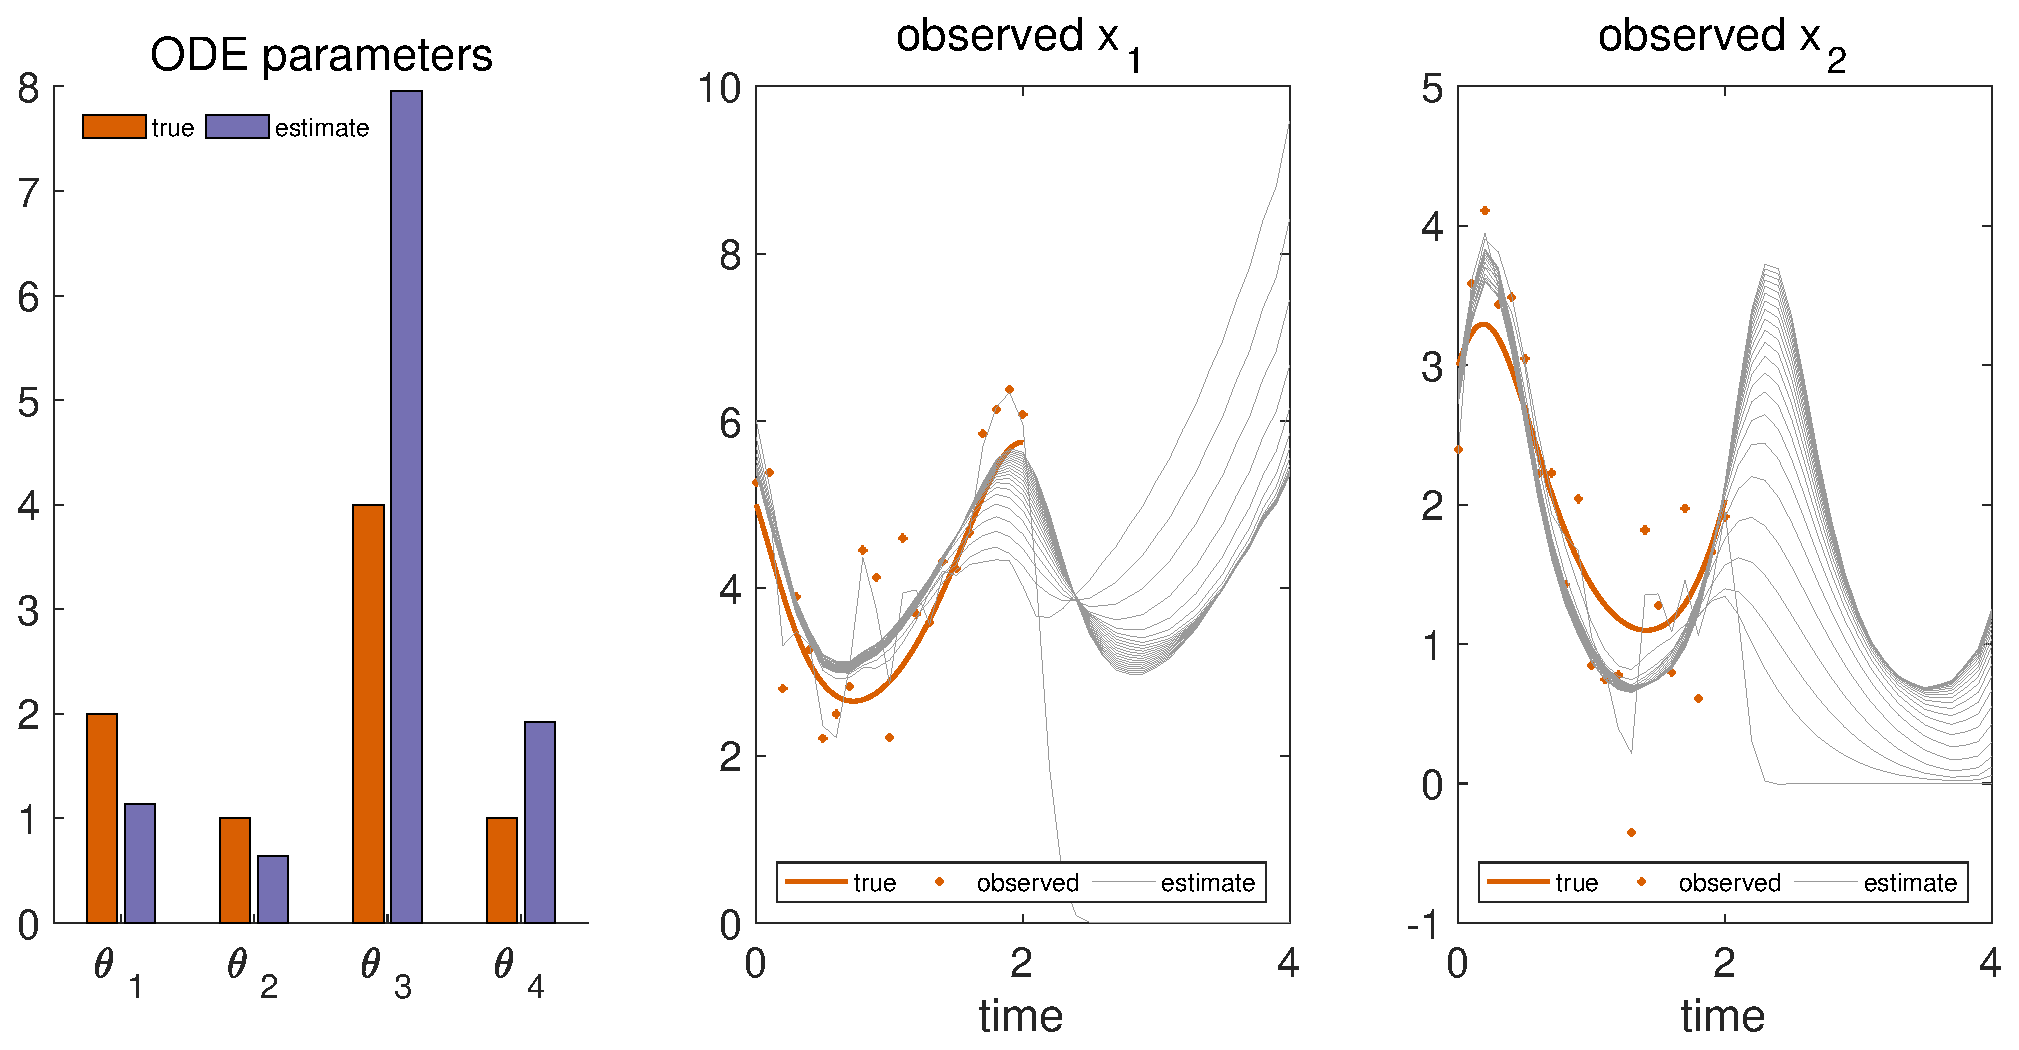
\includegraphics [width=5in]{VGM_for_Lotka_Volterra_23.eps}

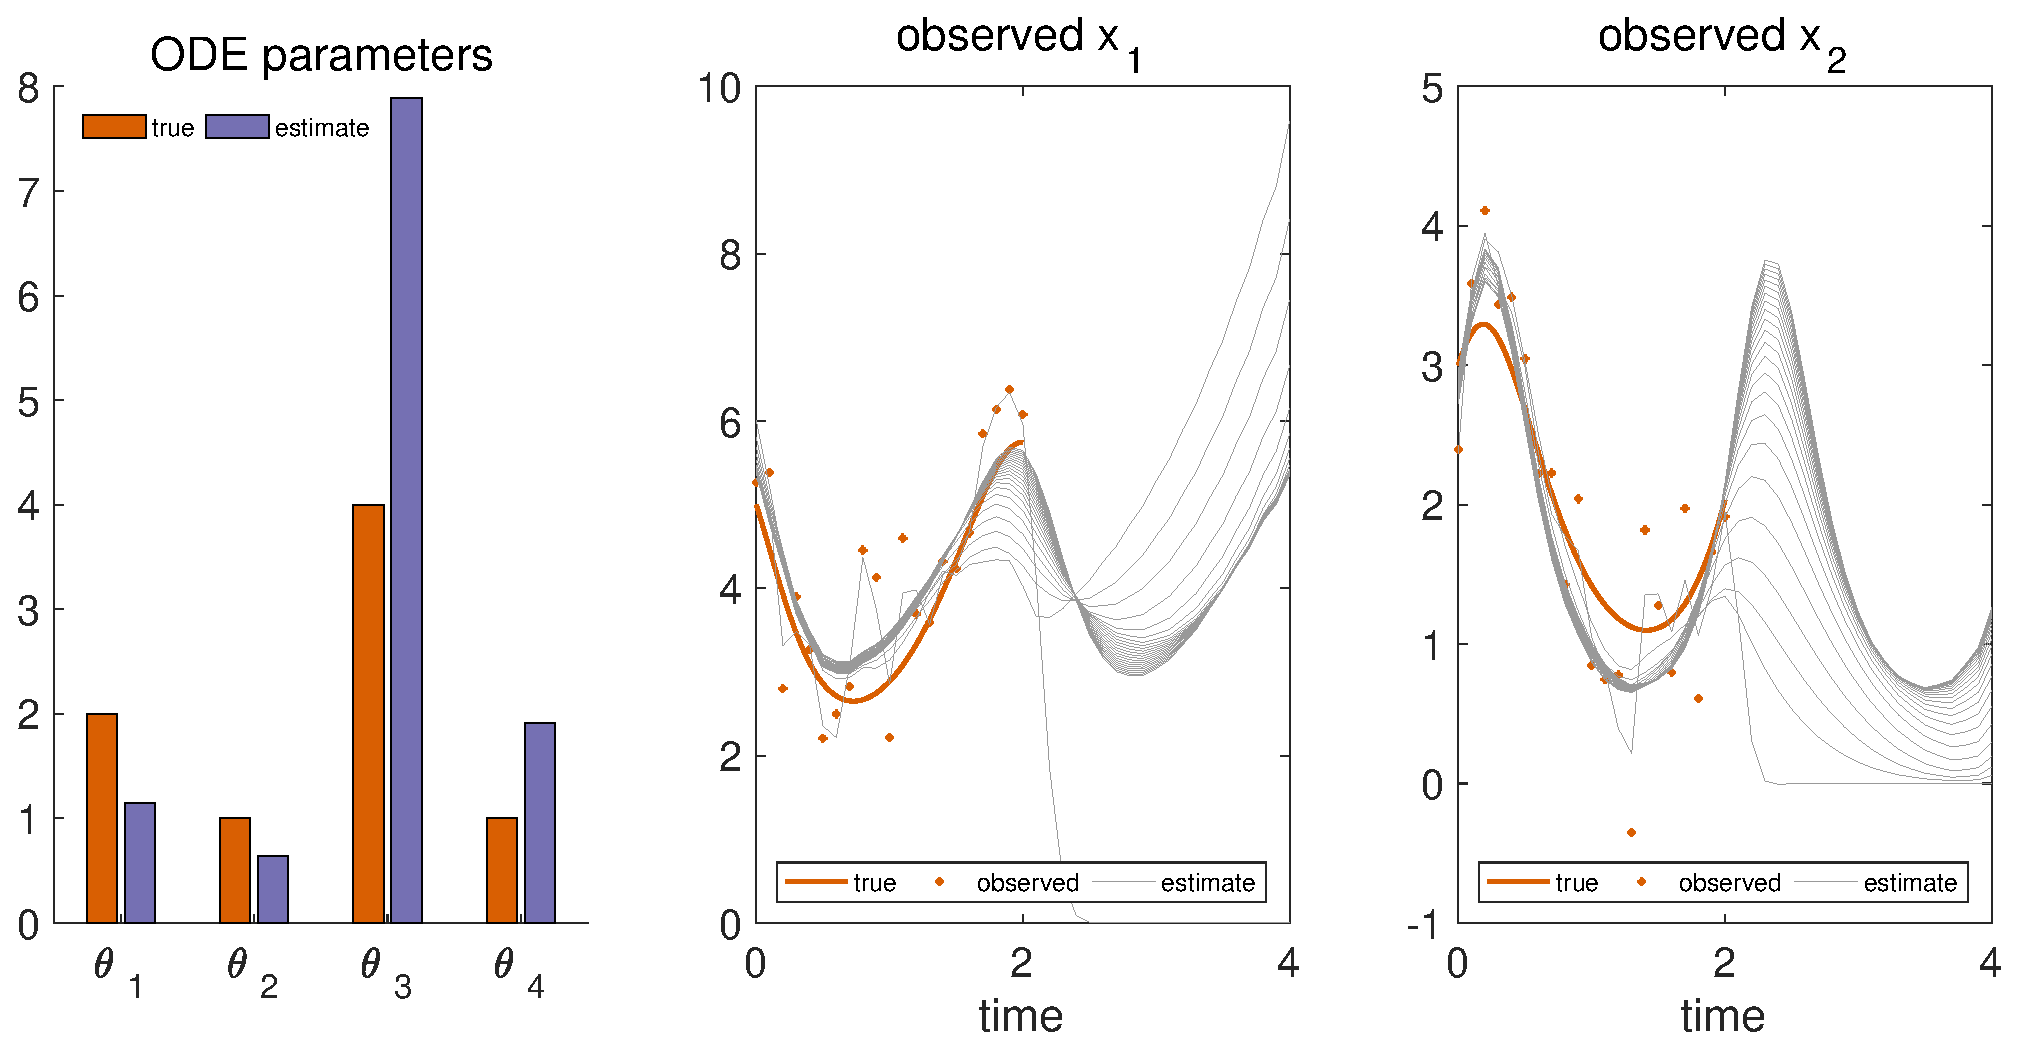
\includegraphics [width=5in]{VGM_for_Lotka_Volterra_24.eps}

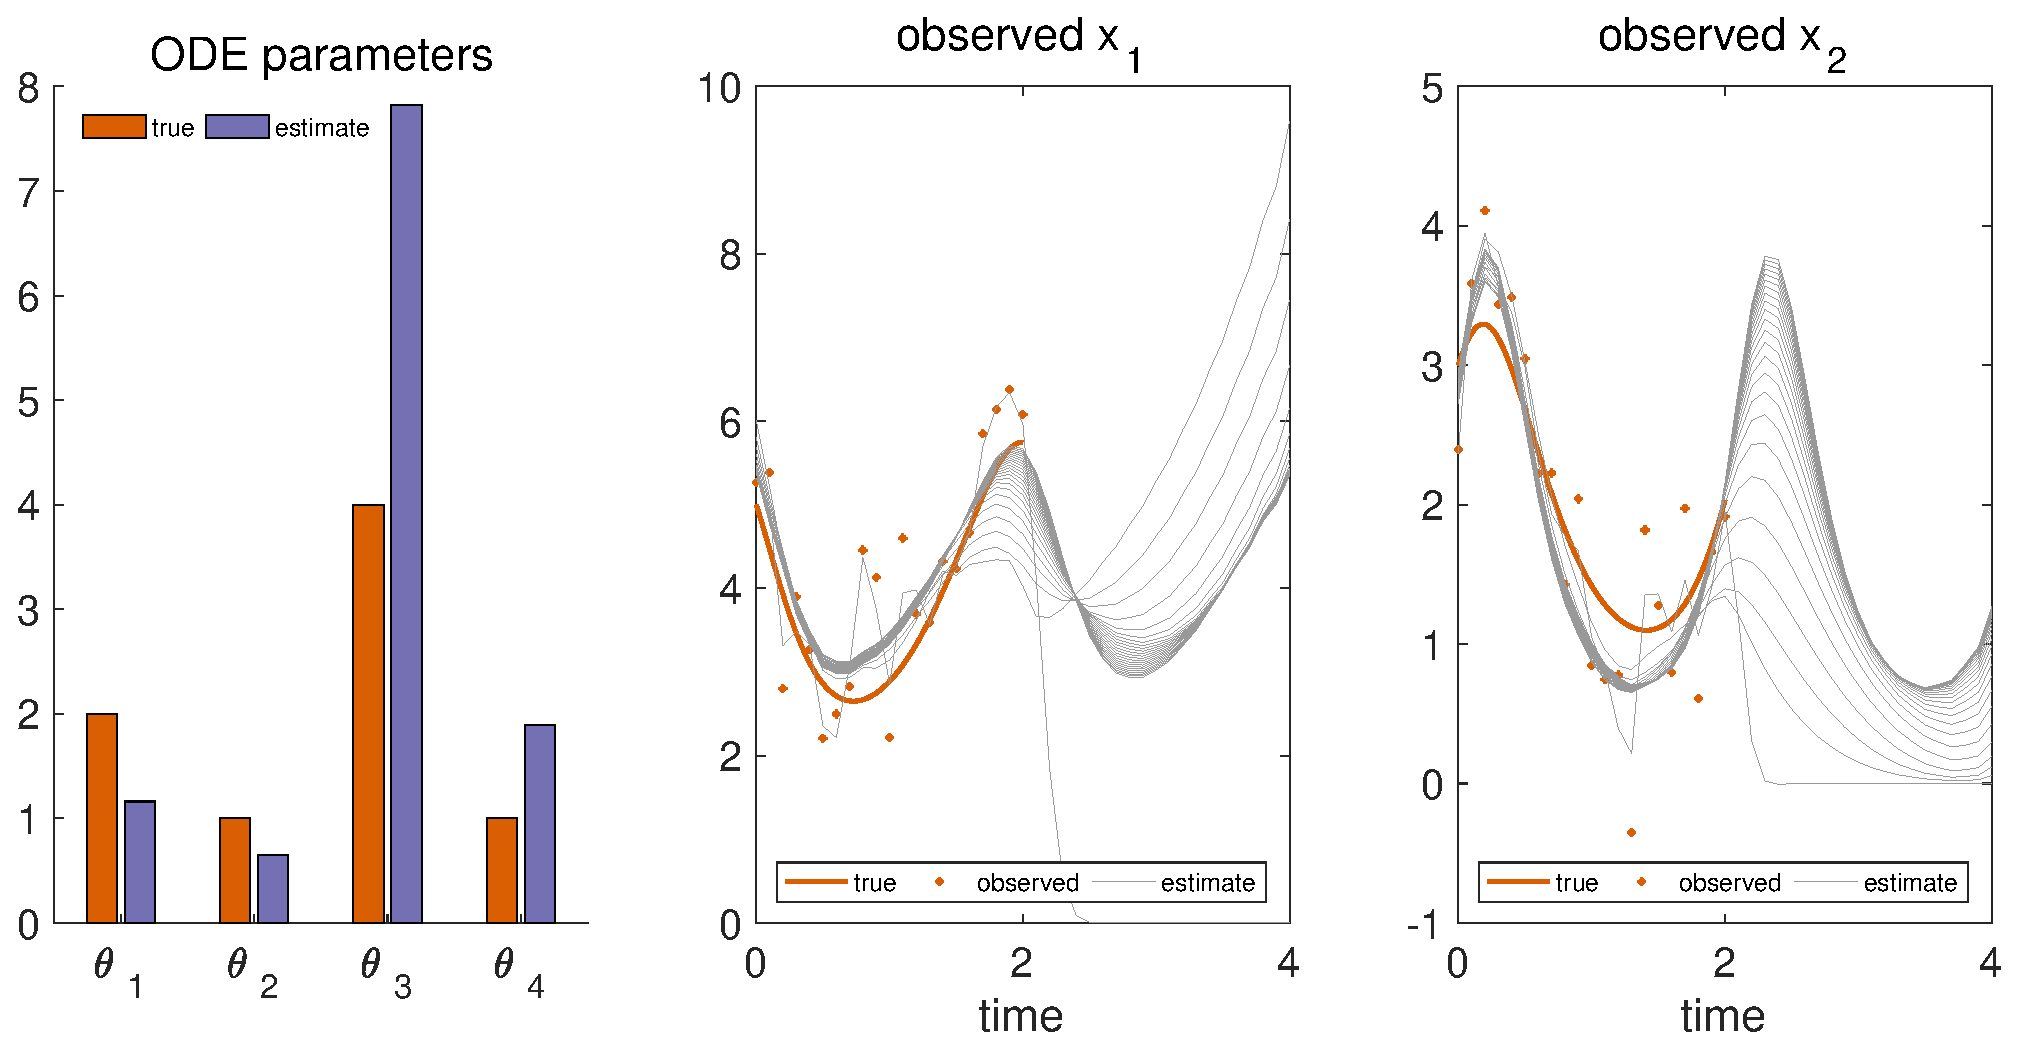
\includegraphics [width=5in]{VGM_for_Lotka_Volterra_25.eps}

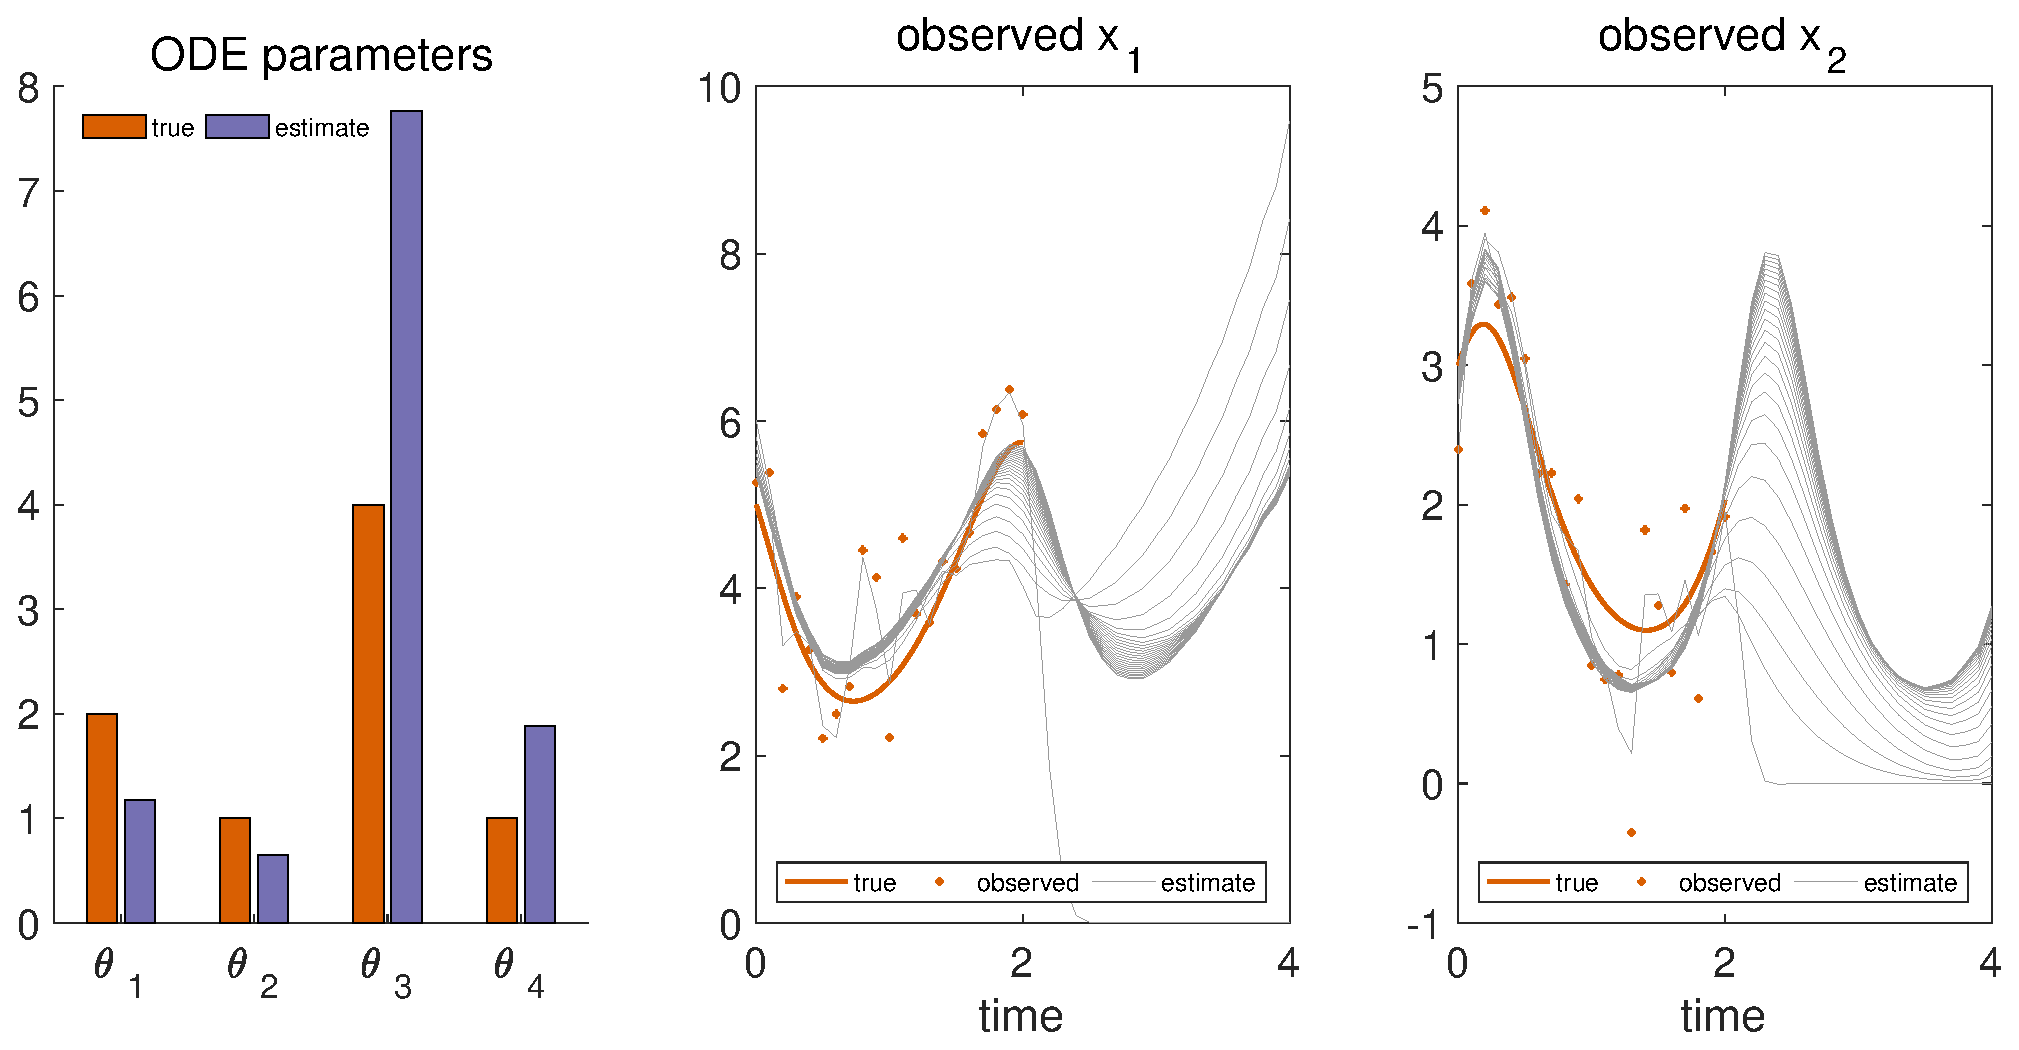
\includegraphics [width=5in]{VGM_for_Lotka_Volterra_26.eps}

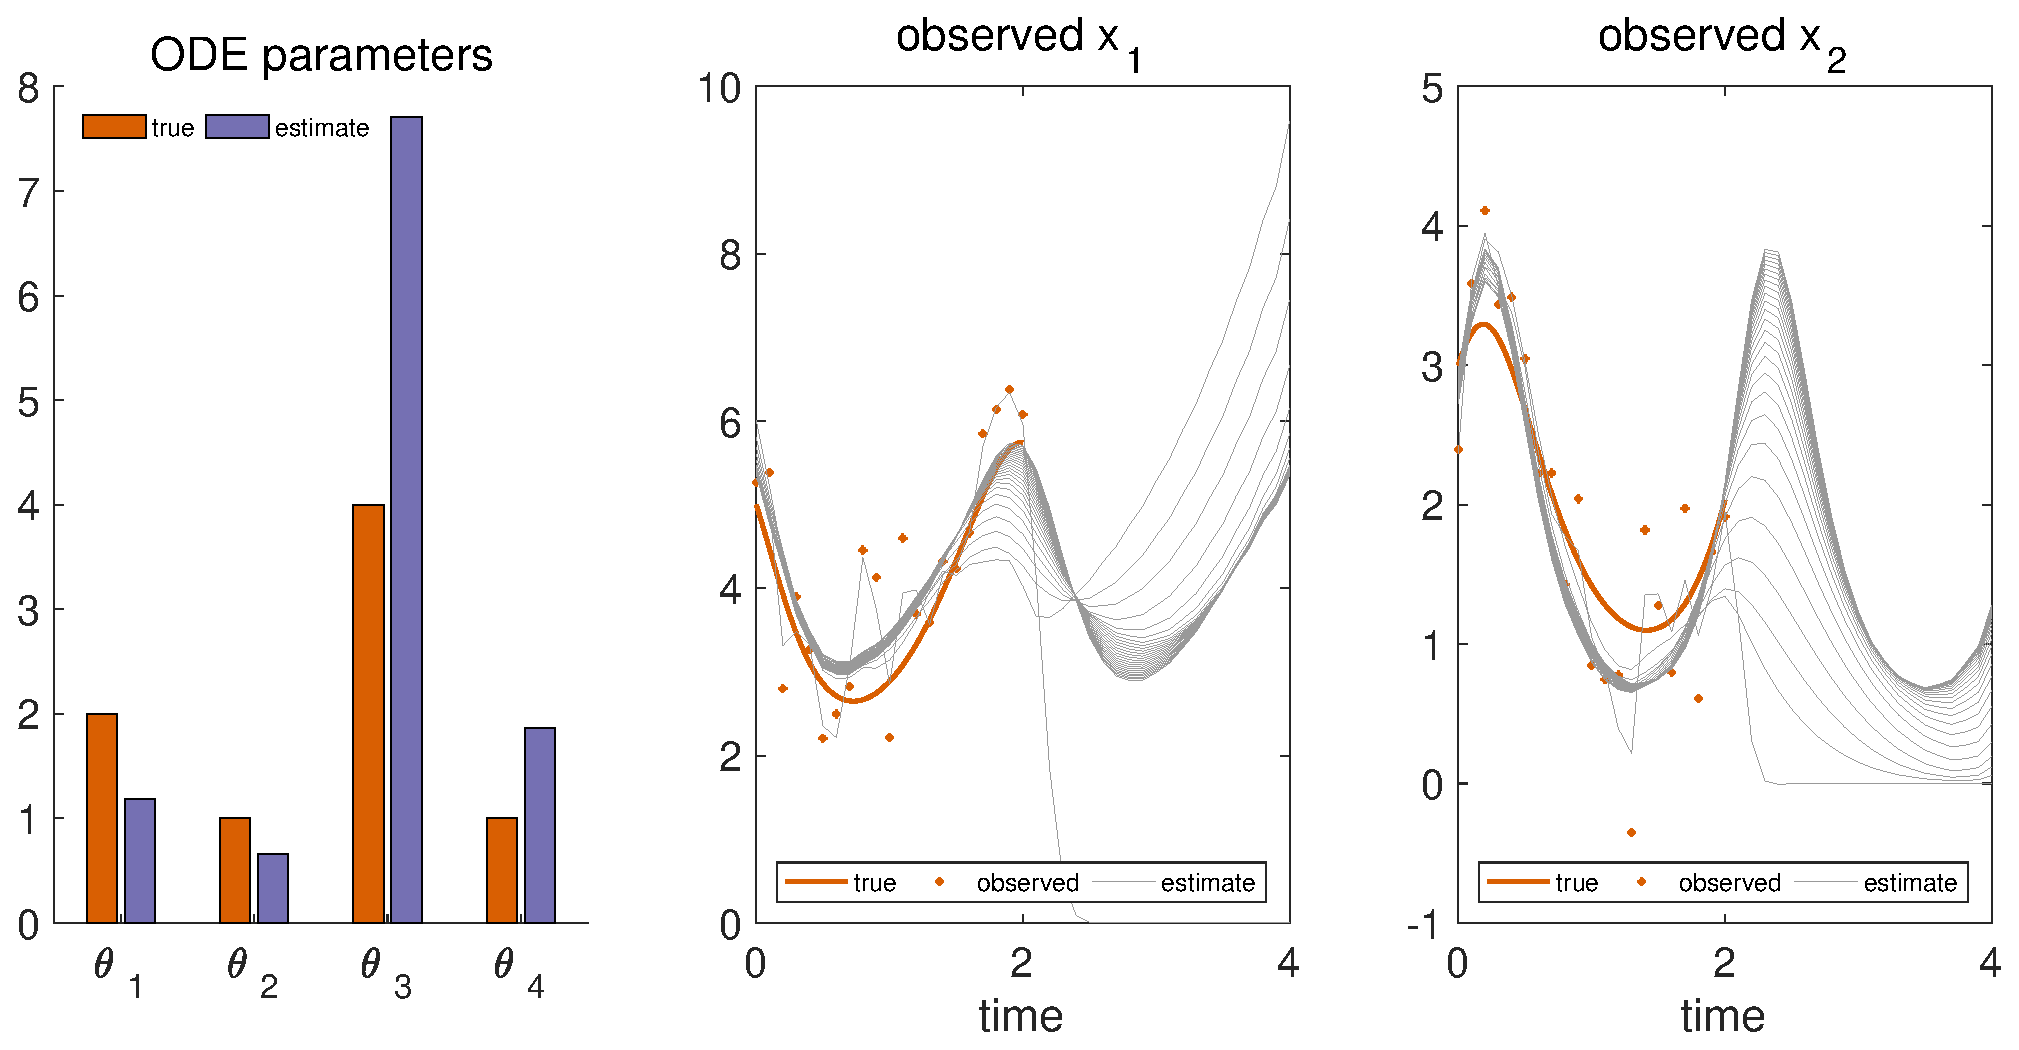
\includegraphics [width=5in]{VGM_for_Lotka_Volterra_27.eps}

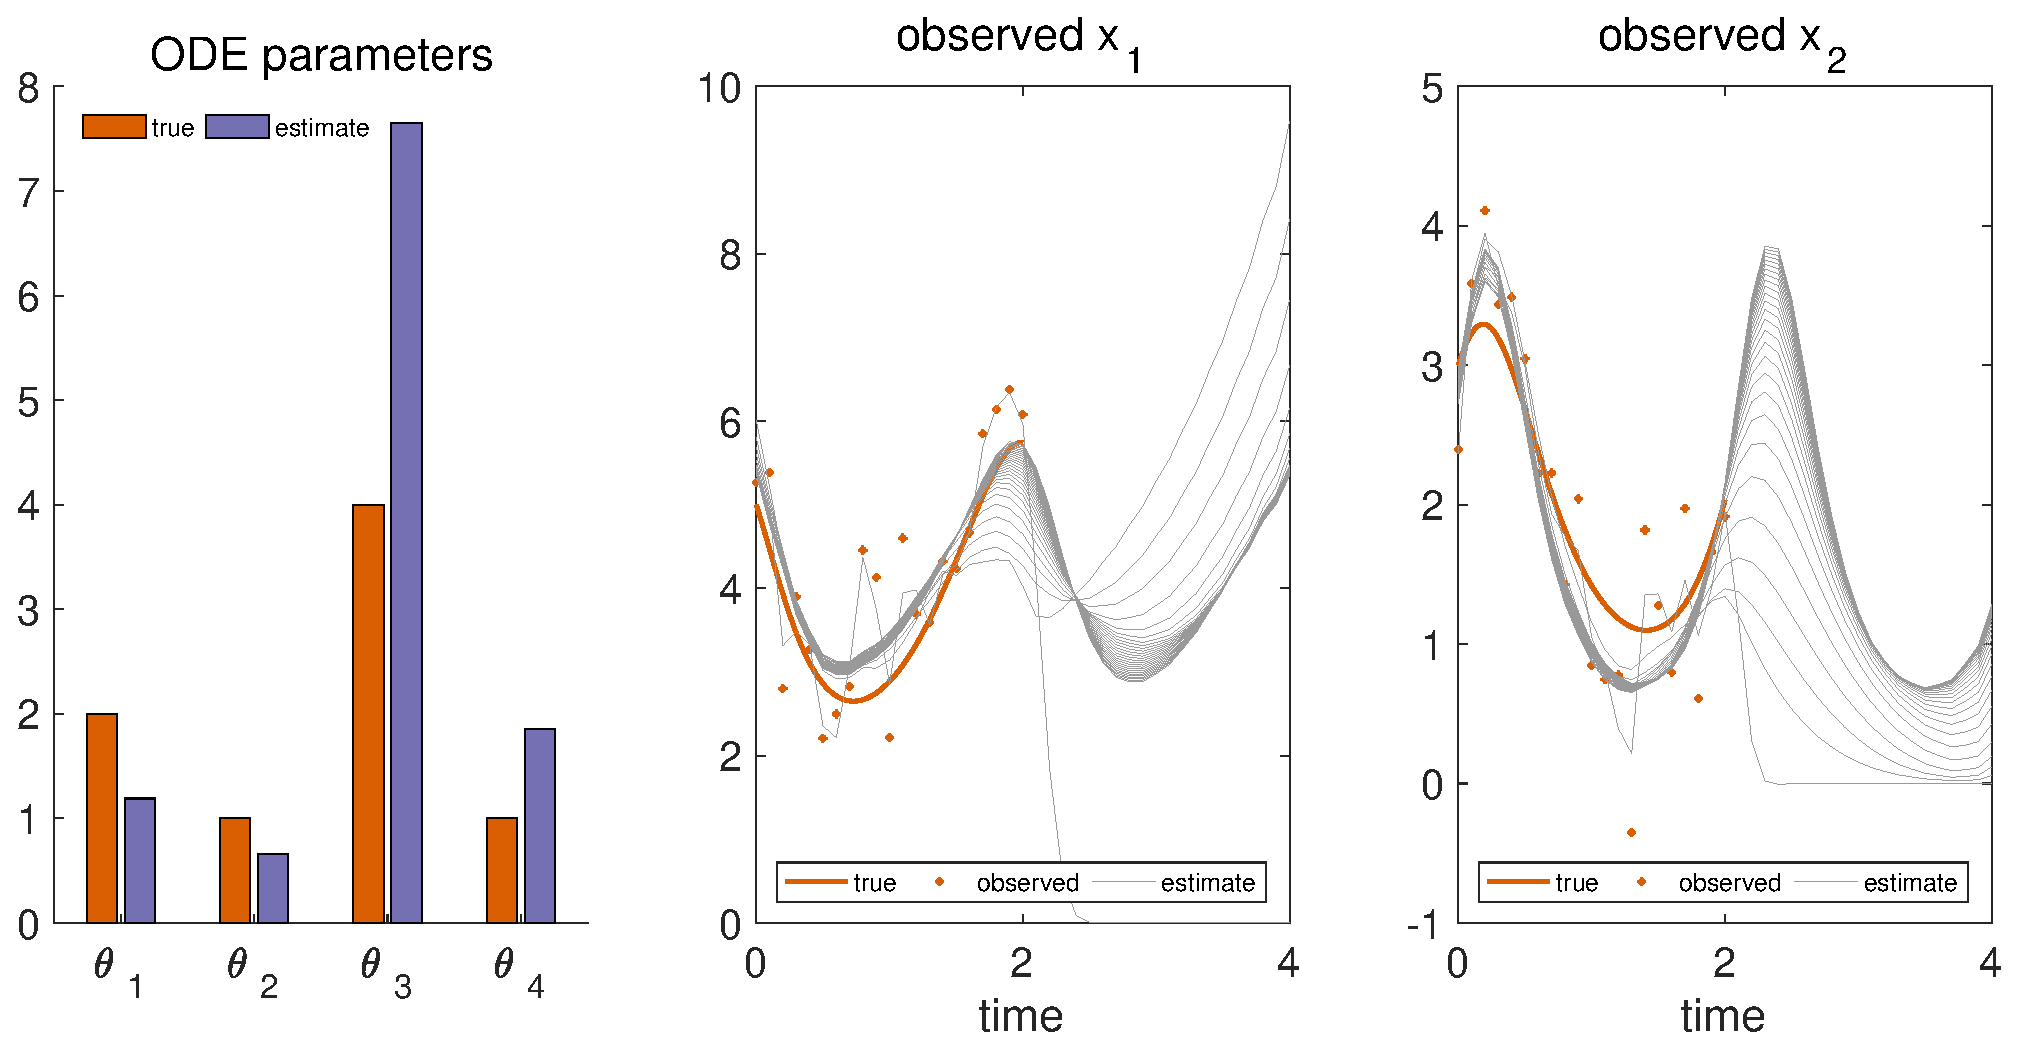
\includegraphics [width=5in]{VGM_for_Lotka_Volterra_28.eps}

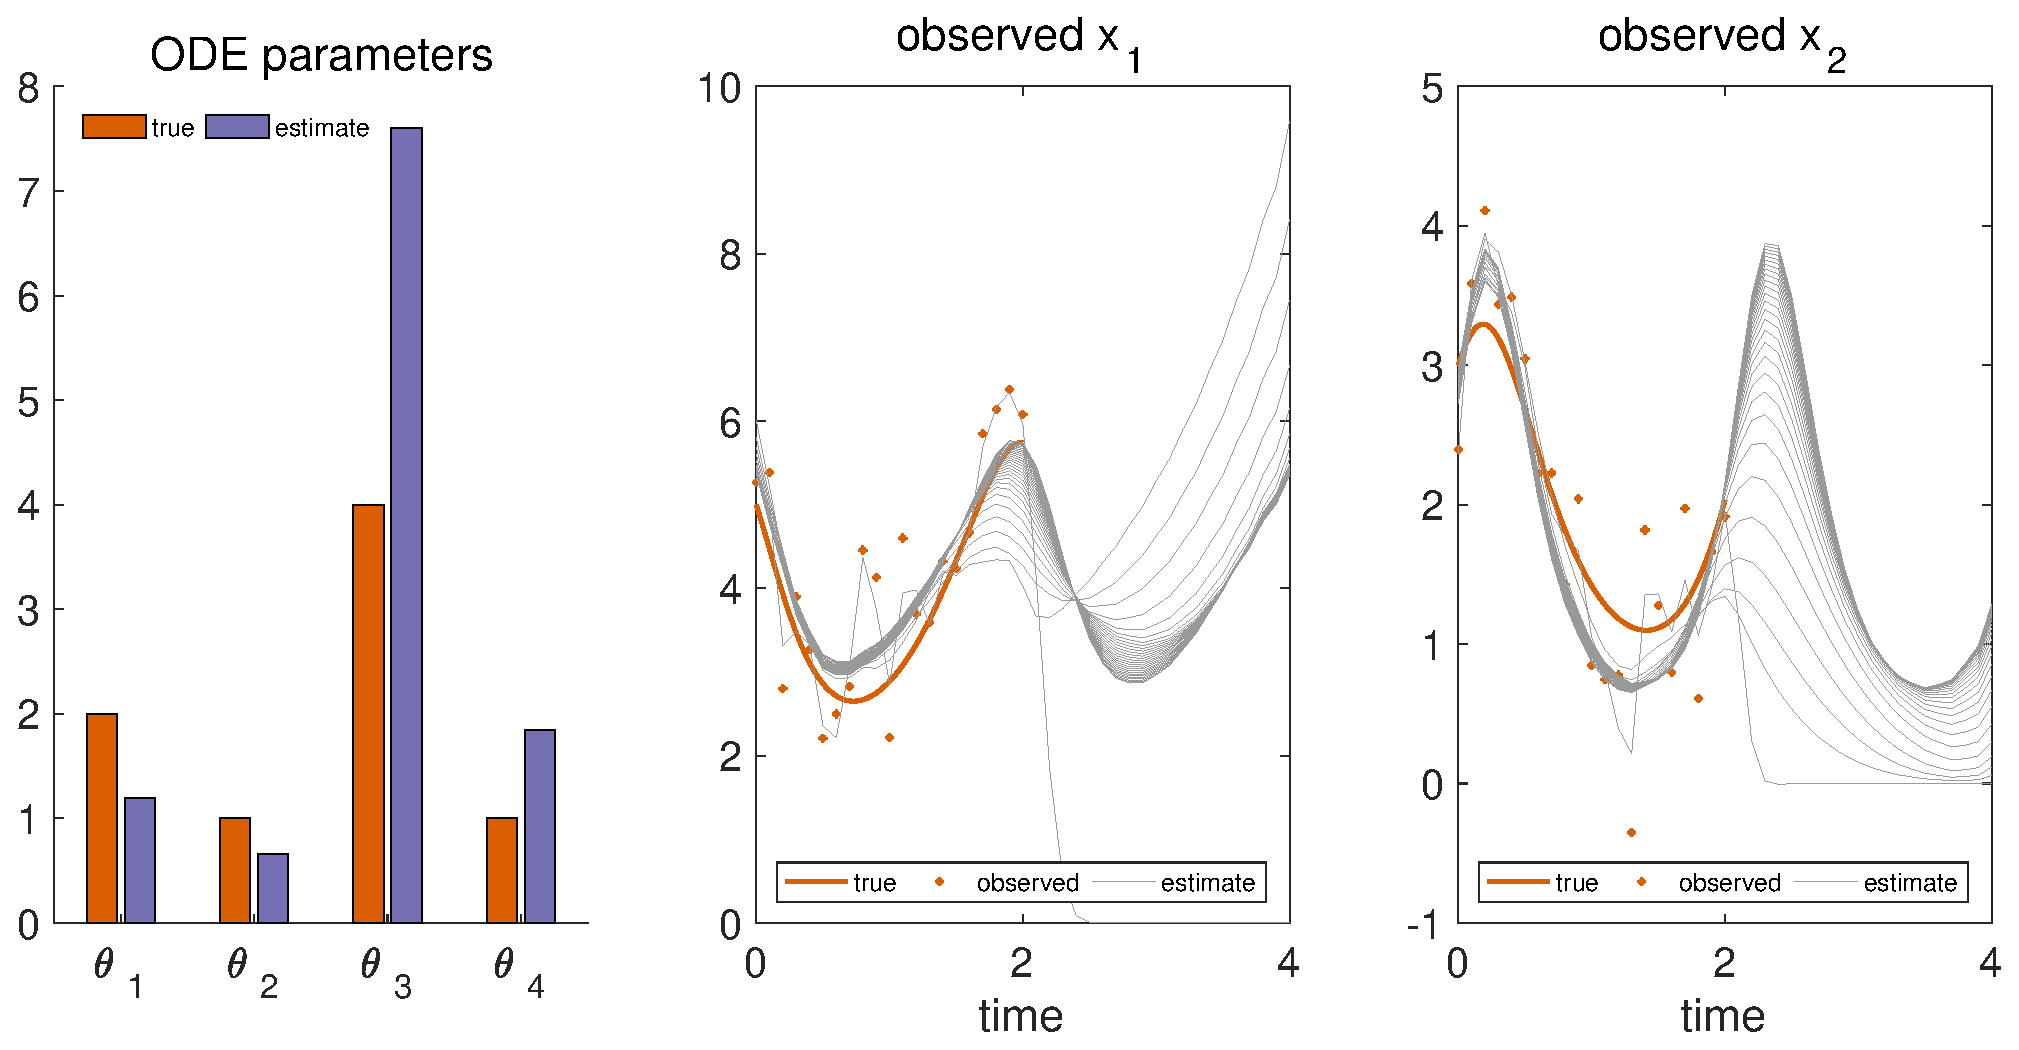
\includegraphics [width=5in]{VGM_for_Lotka_Volterra_29.eps}

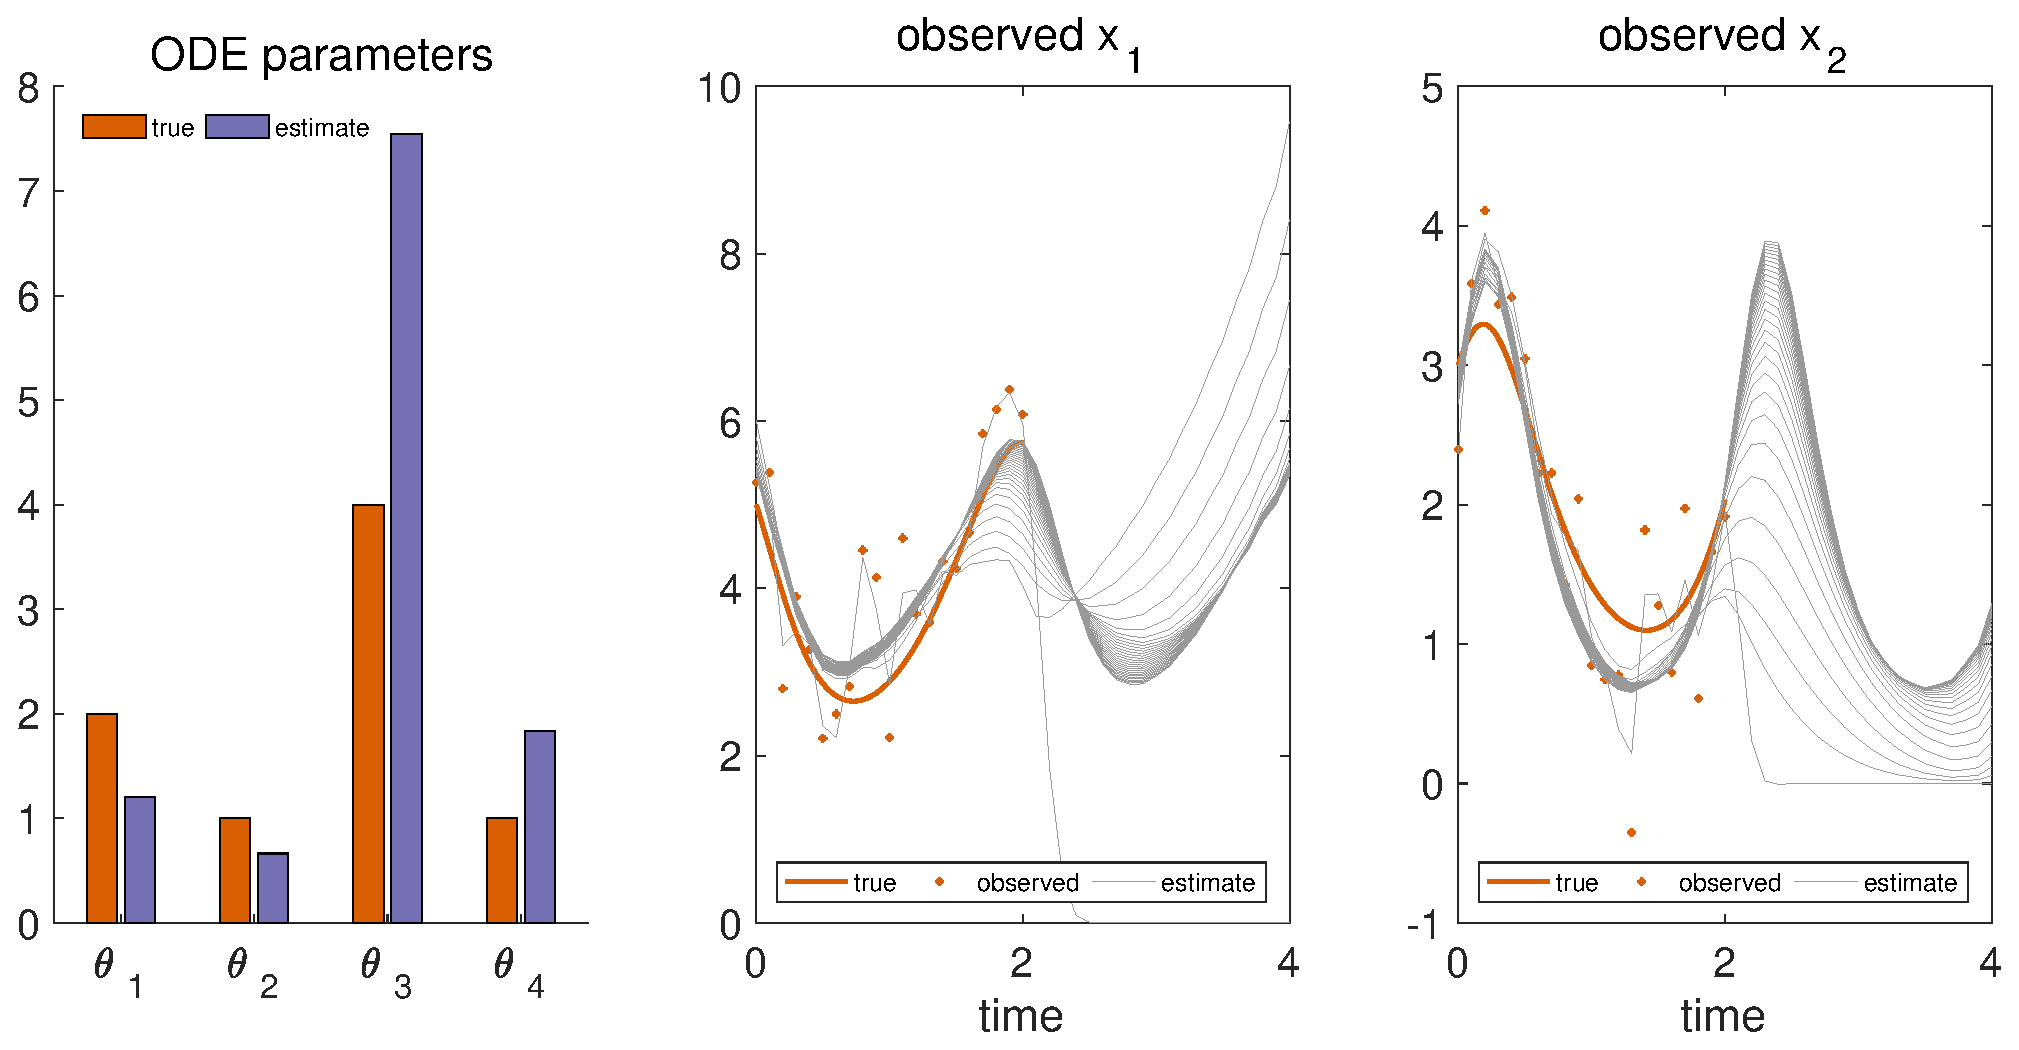
\includegraphics [width=5in]{VGM_for_Lotka_Volterra_30.eps}

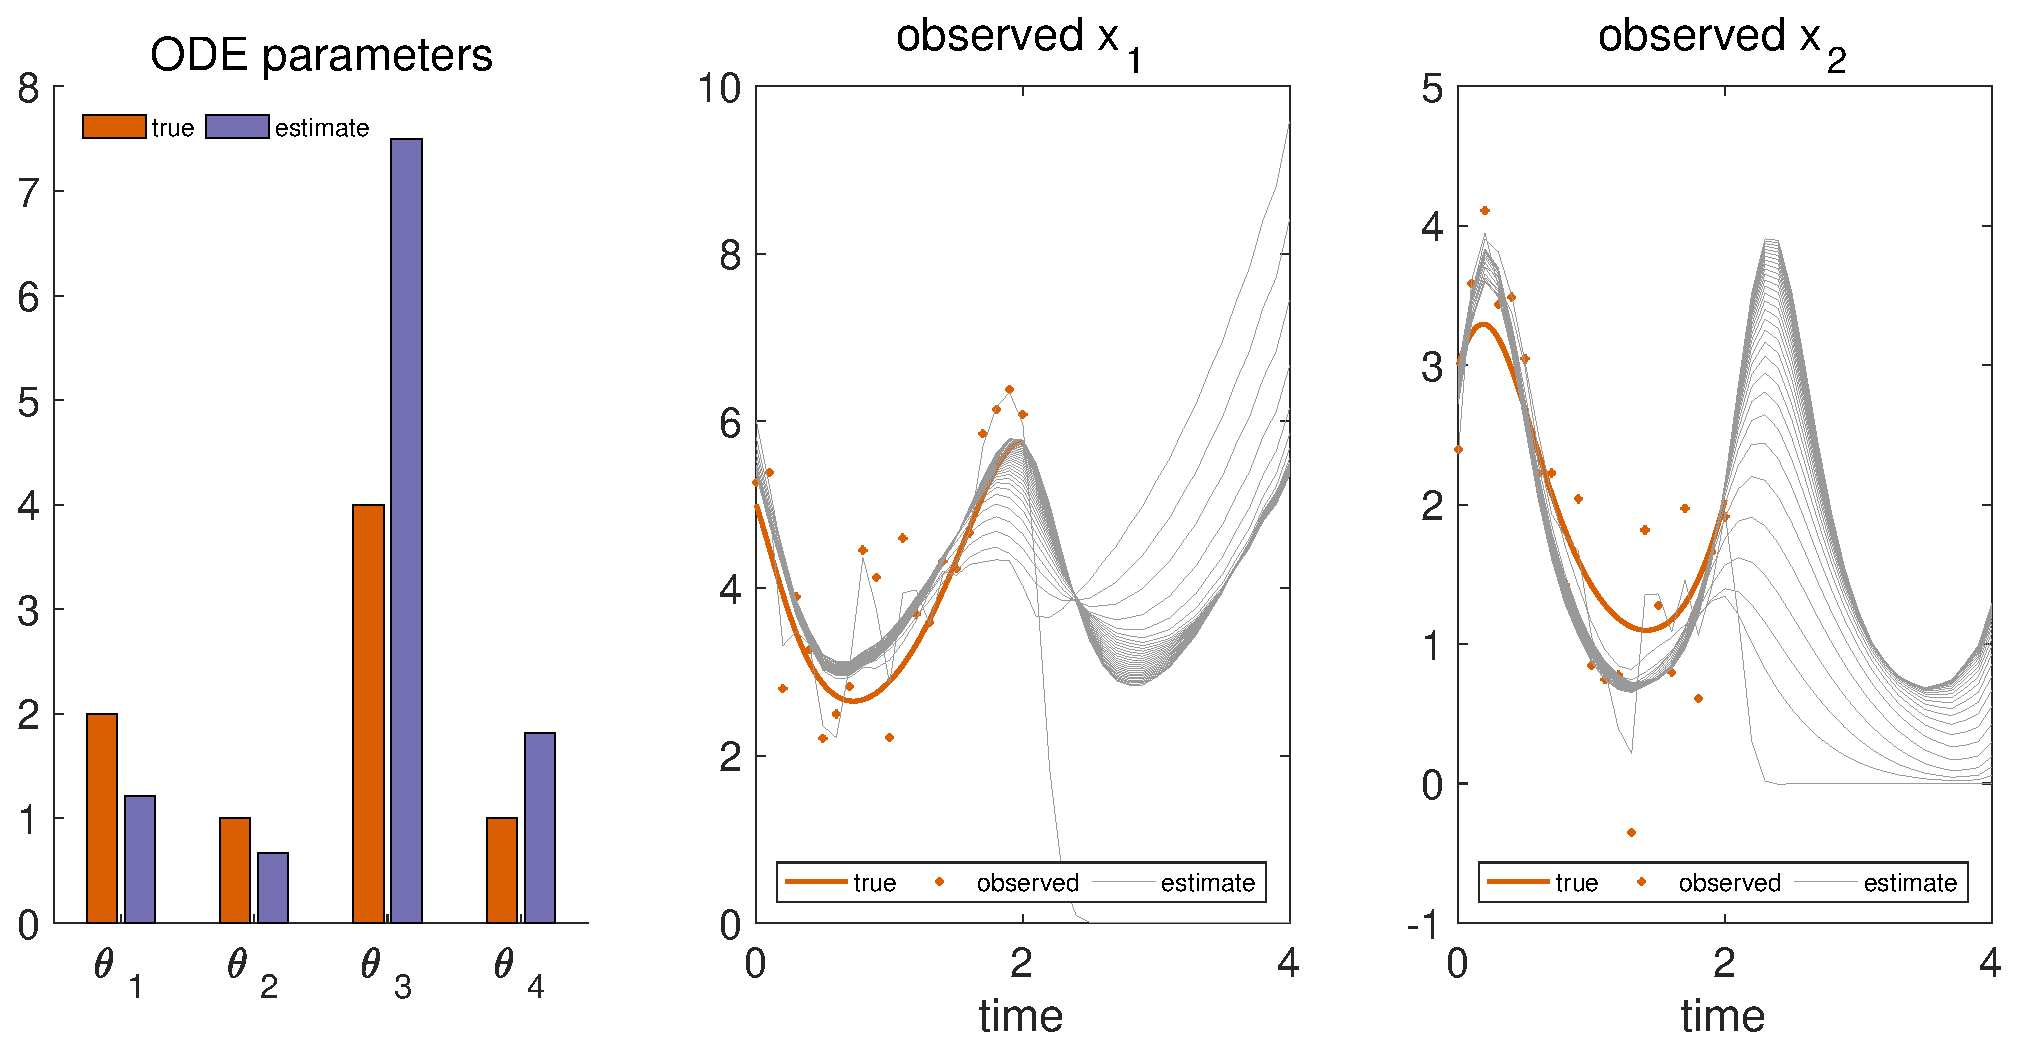
\includegraphics [width=5in]{VGM_for_Lotka_Volterra_31.eps}

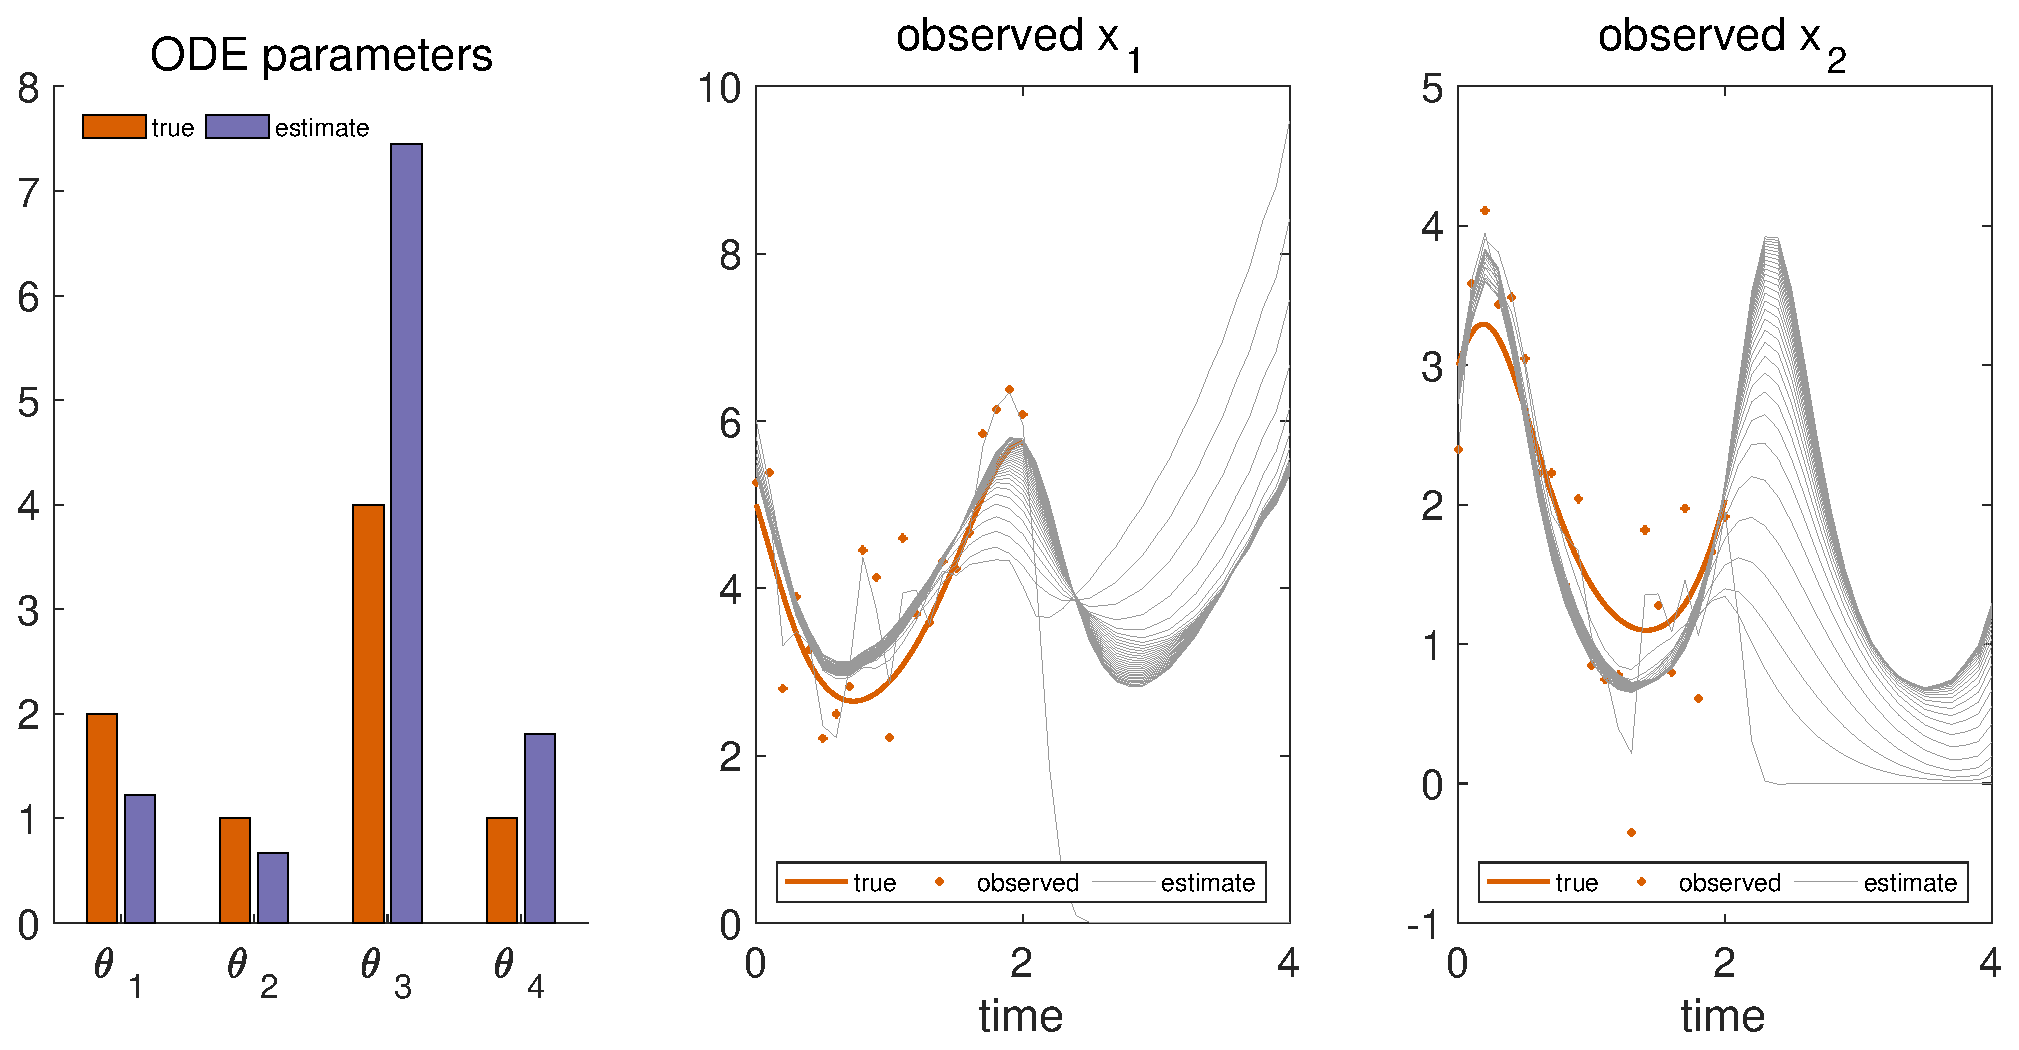
\includegraphics [width=5in]{VGM_for_Lotka_Volterra_32.eps}

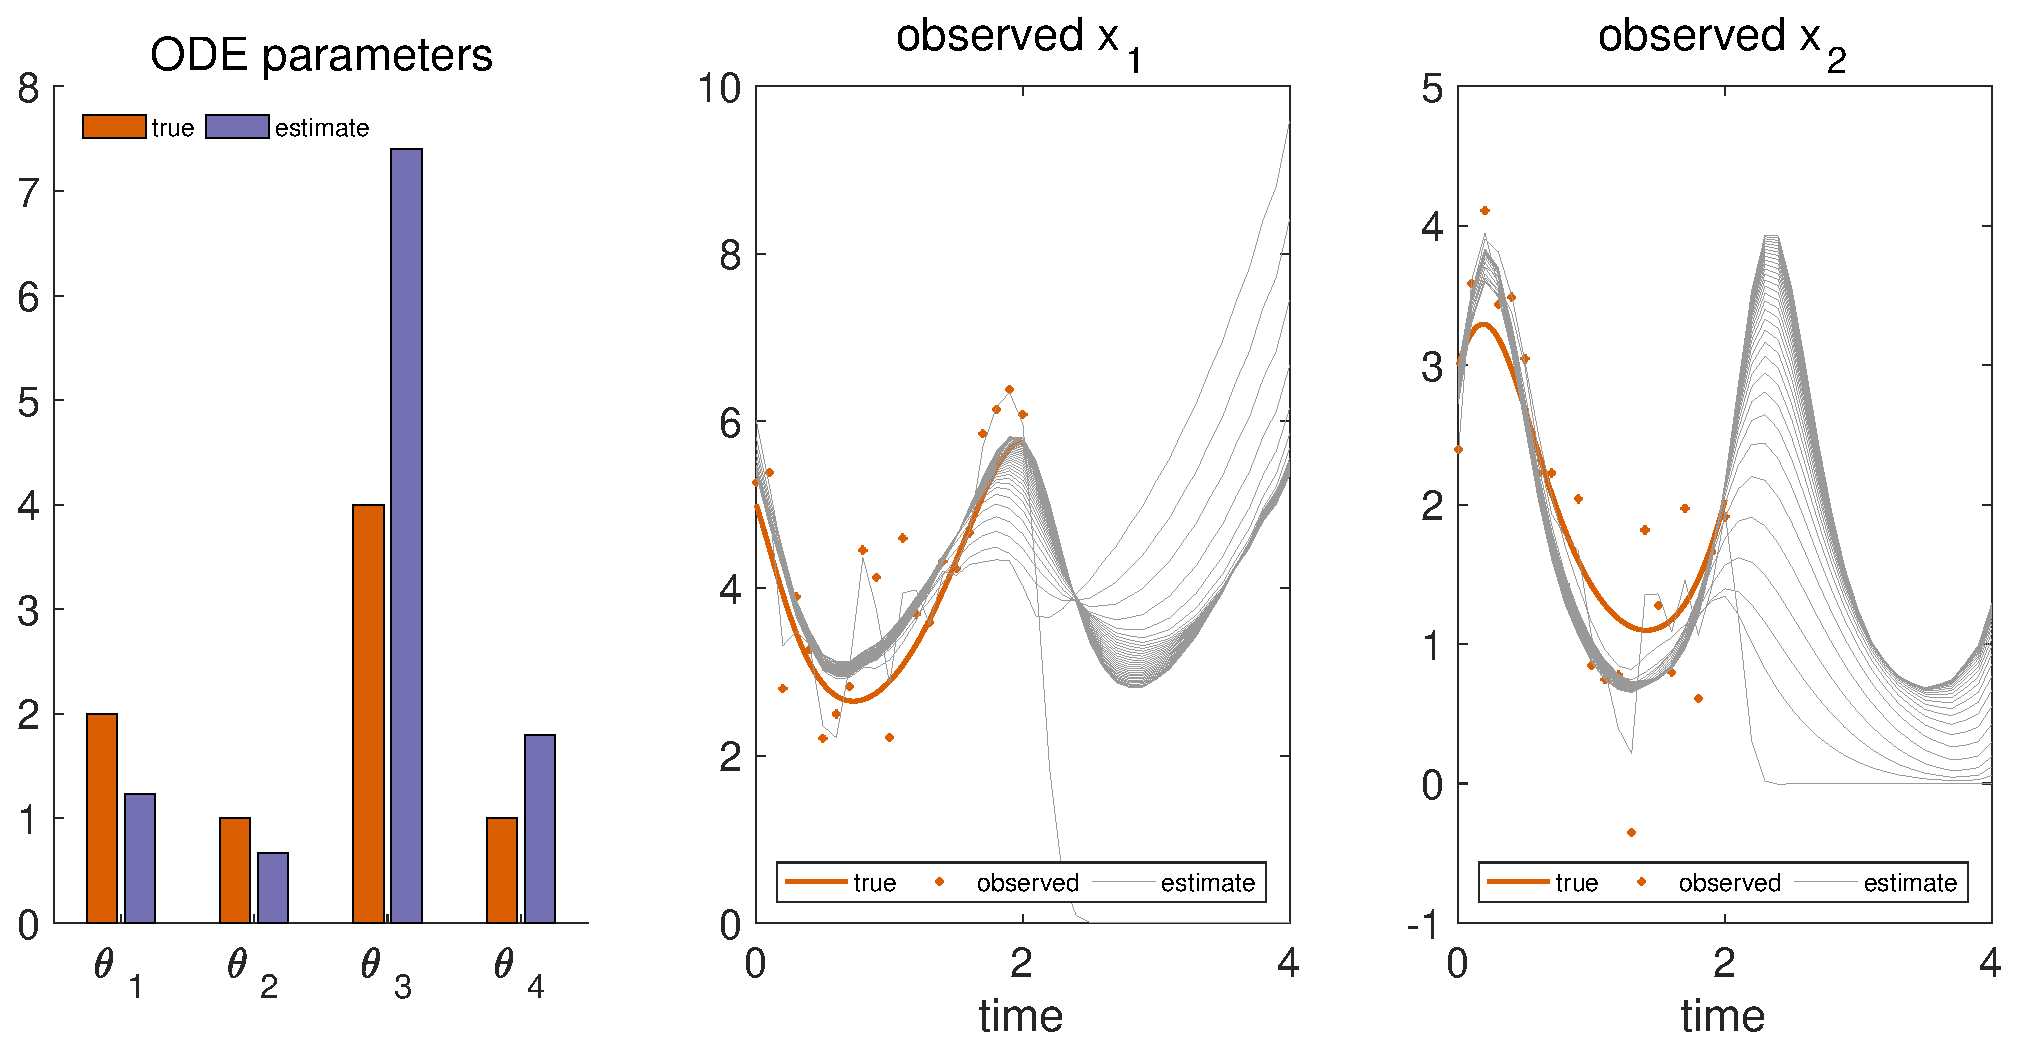
\includegraphics [width=5in]{VGM_for_Lotka_Volterra_33.eps}

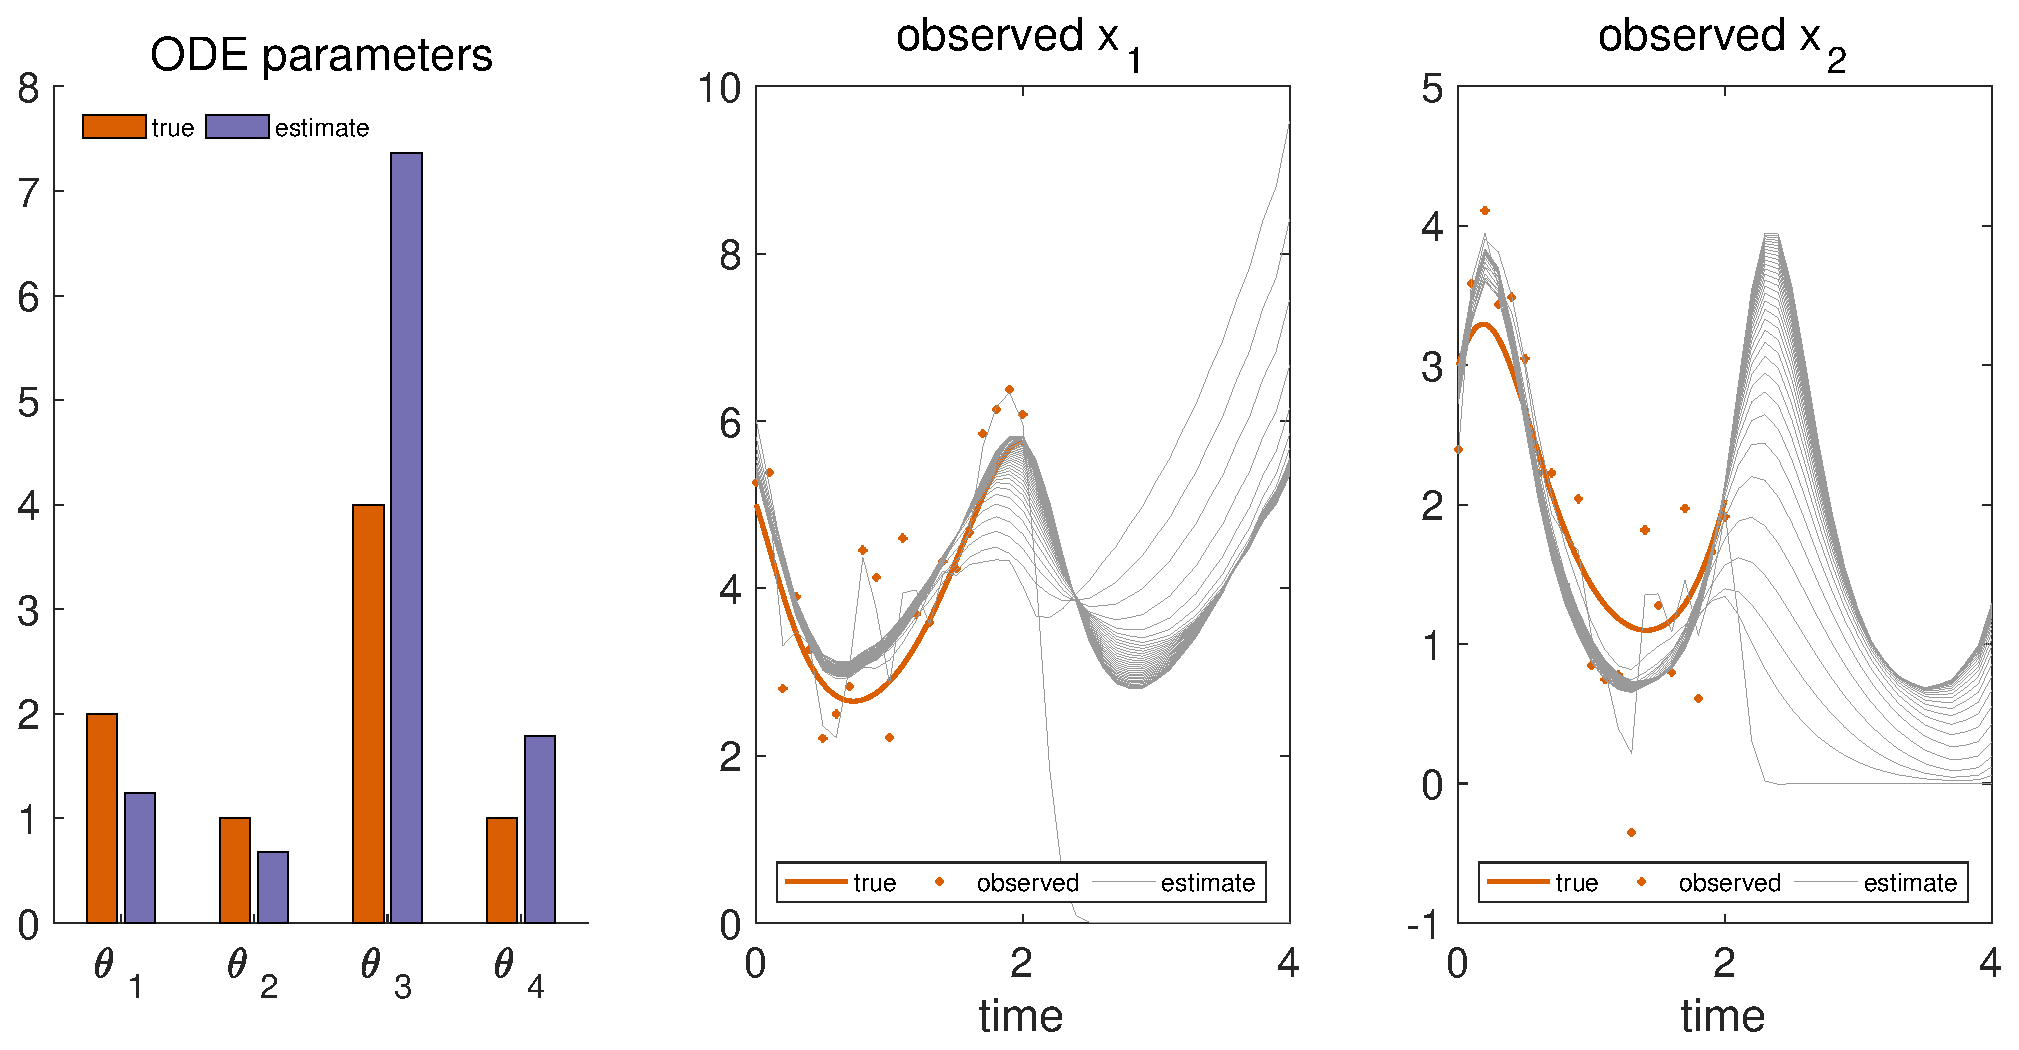
\includegraphics [width=5in]{VGM_for_Lotka_Volterra_34.eps}

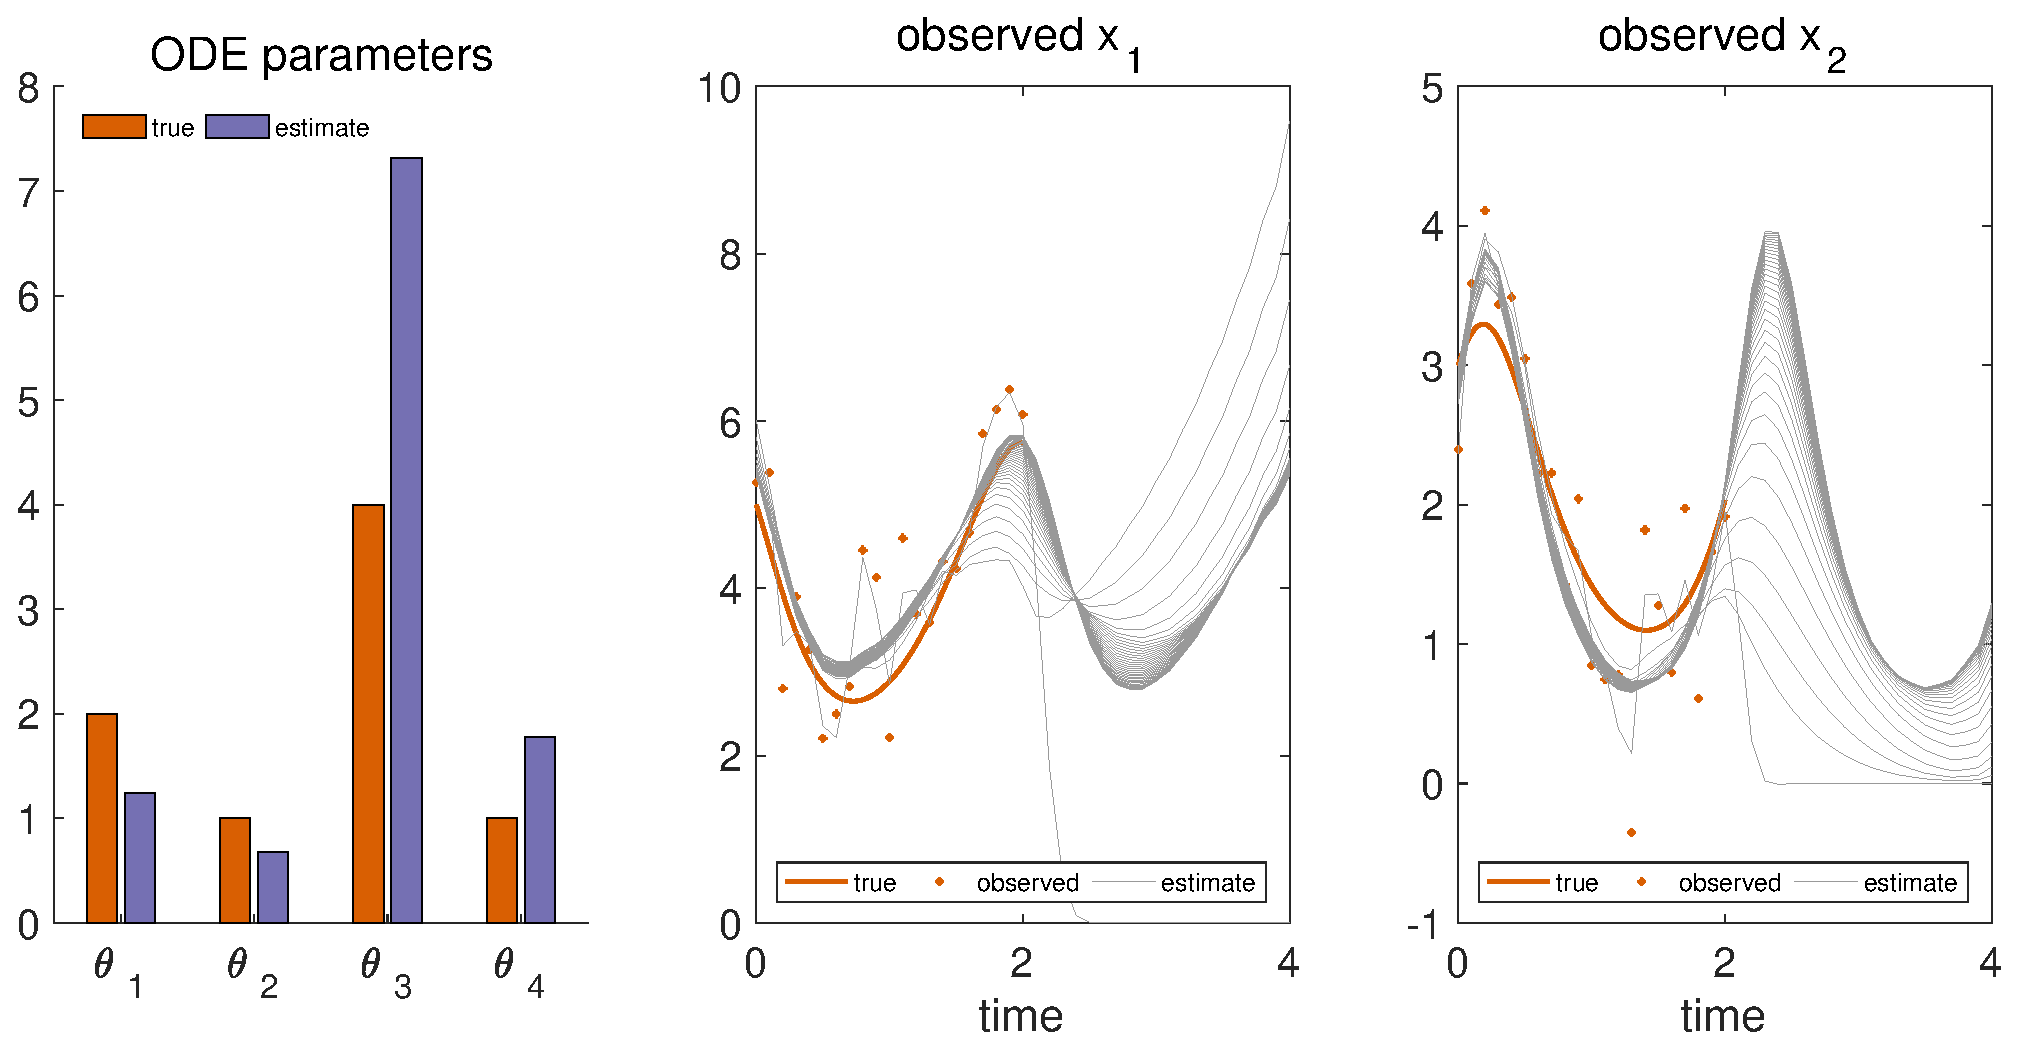
\includegraphics [width=5in]{VGM_for_Lotka_Volterra_35.eps}

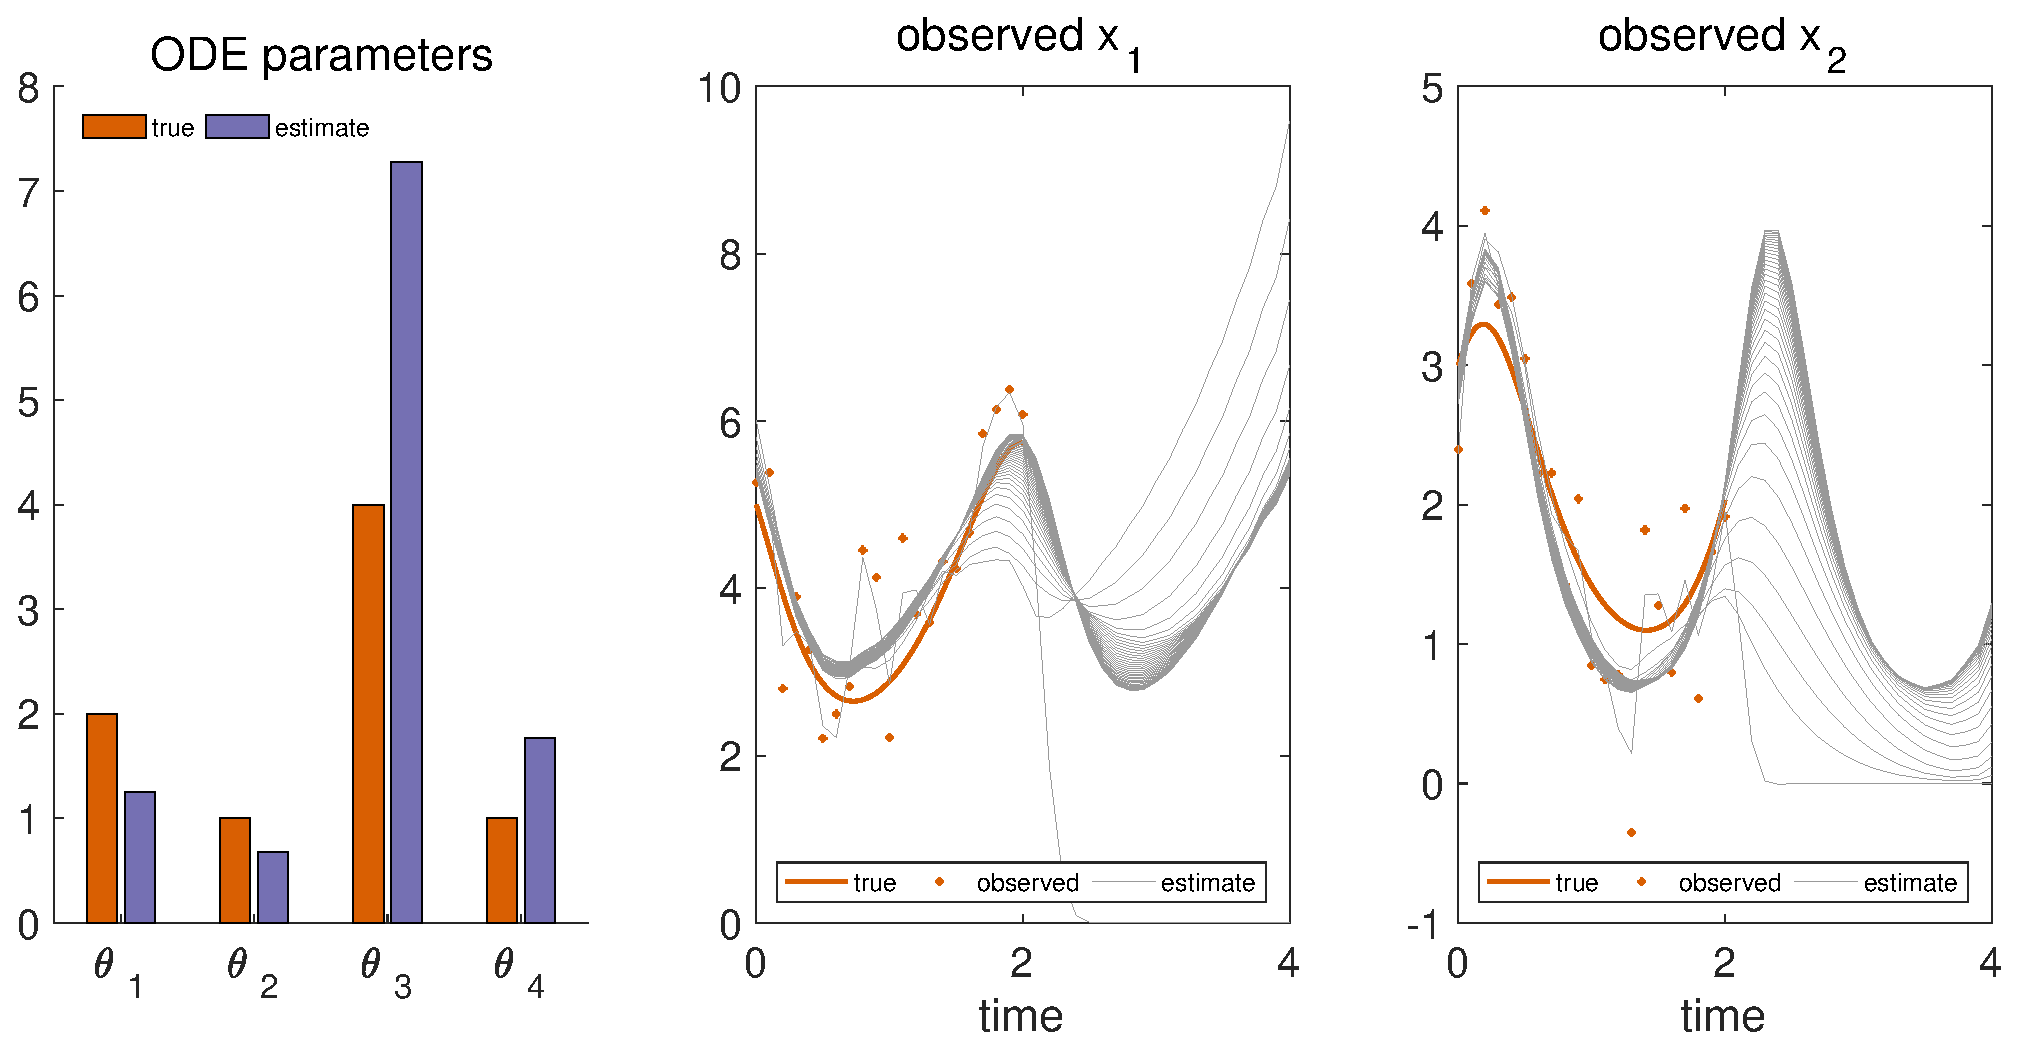
\includegraphics [width=5in]{VGM_for_Lotka_Volterra_36.eps}

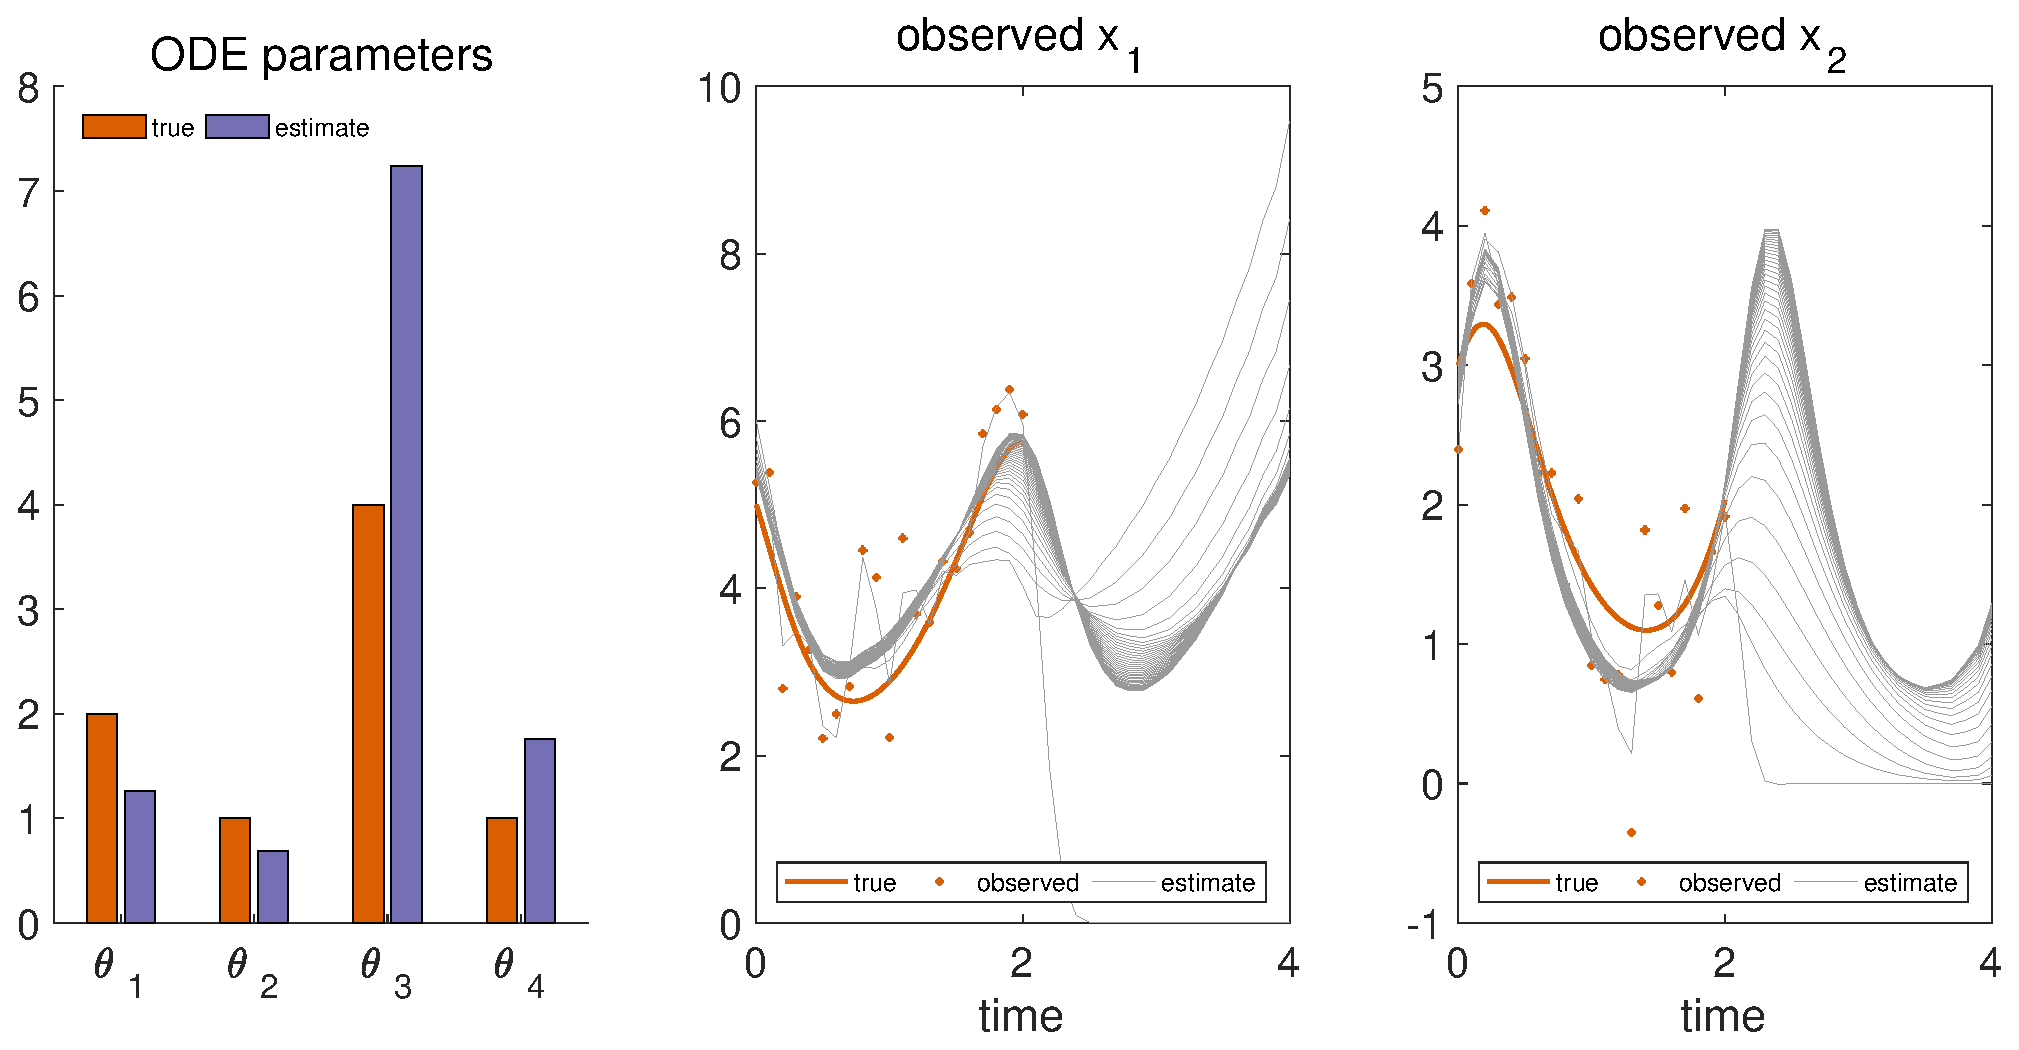
\includegraphics [width=5in]{VGM_for_Lotka_Volterra_37.eps}

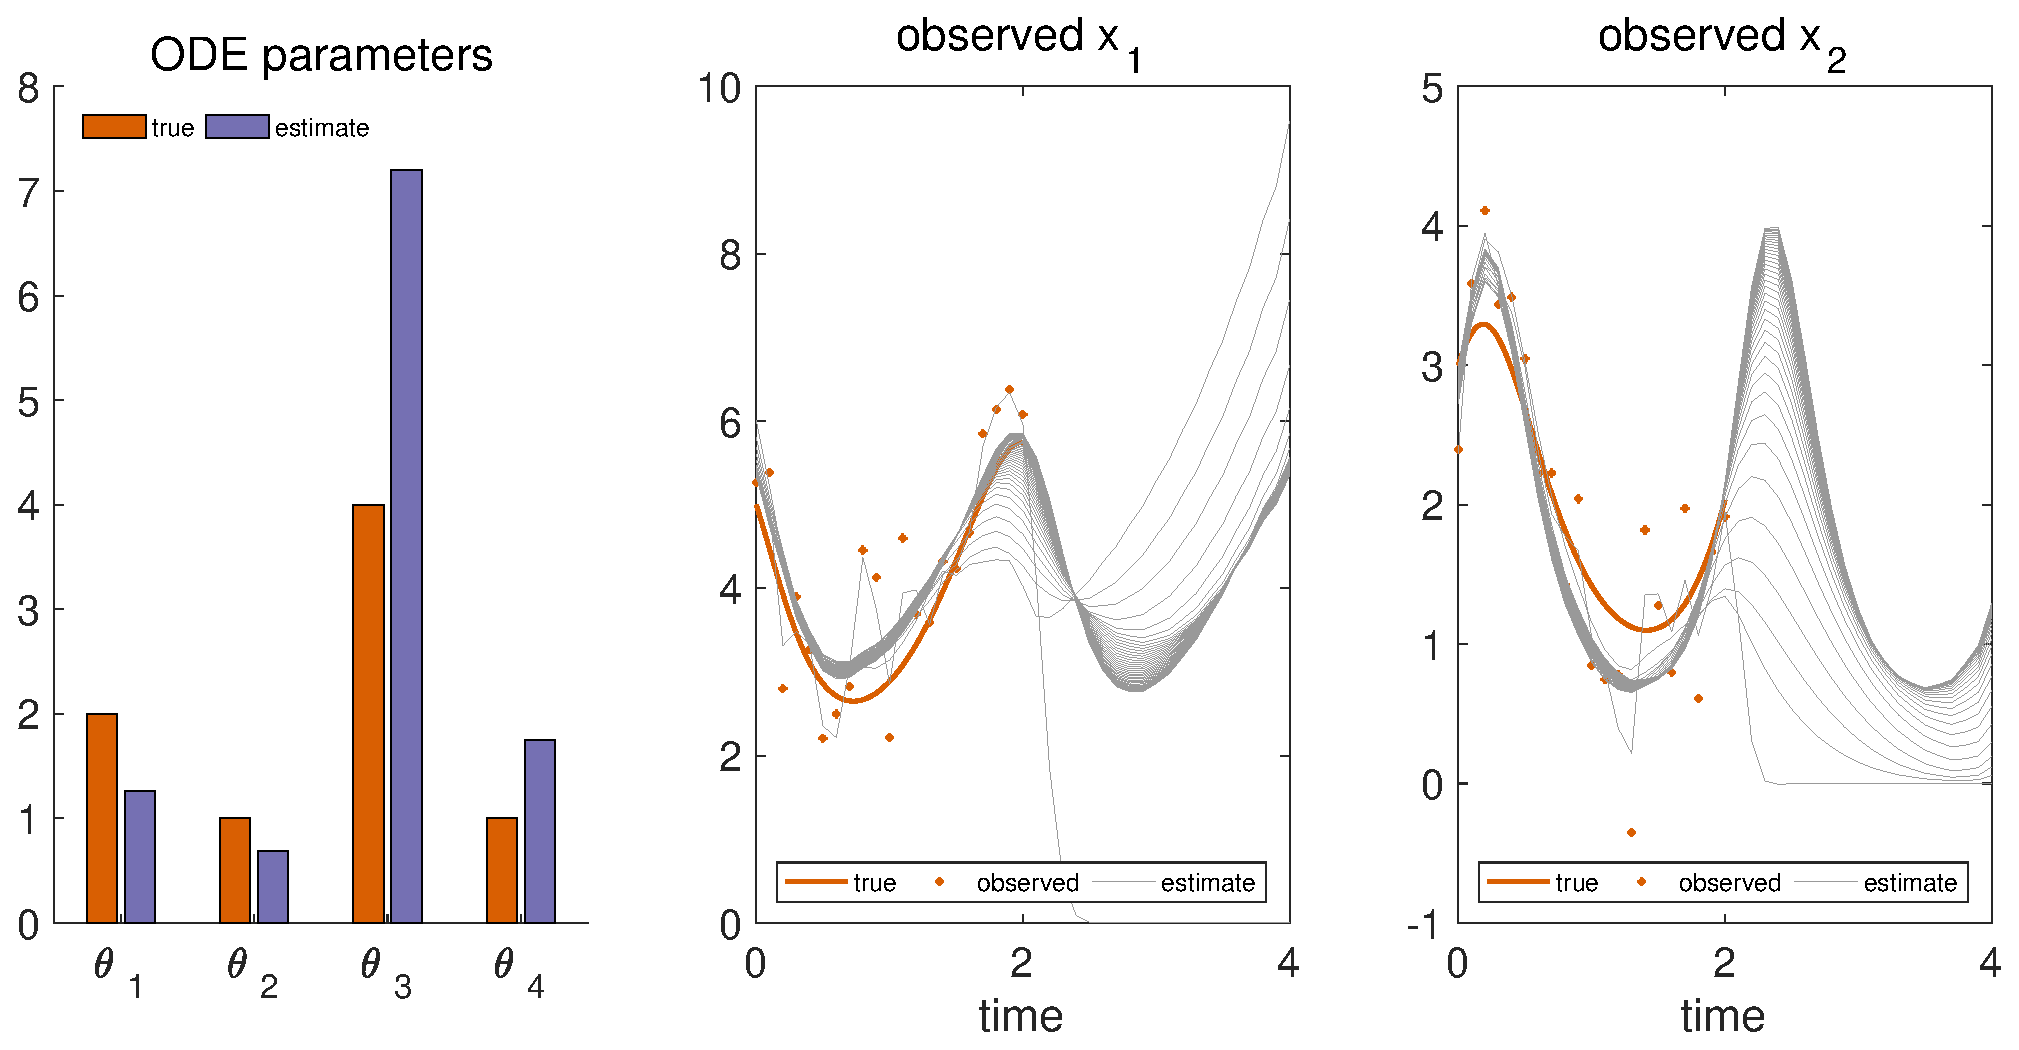
\includegraphics [width=5in]{VGM_for_Lotka_Volterra_38.eps}

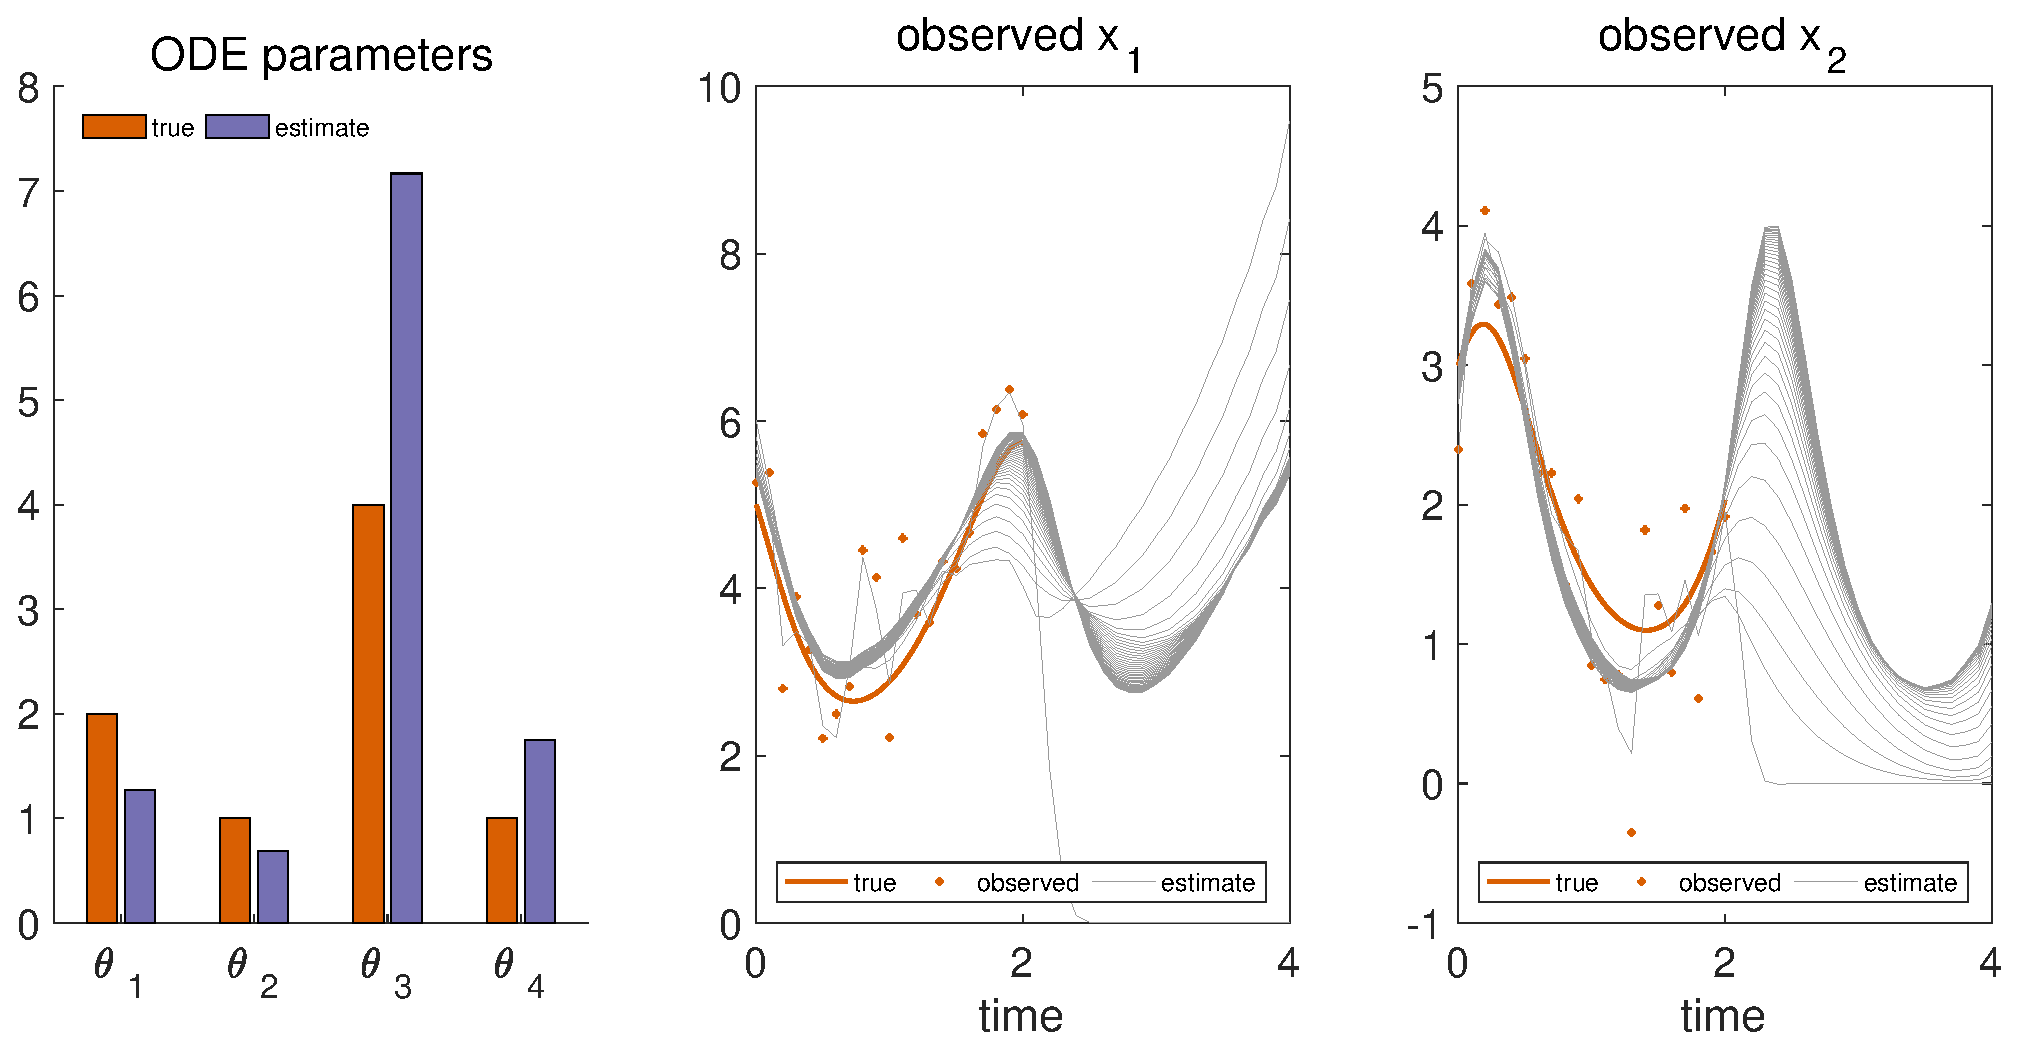
\includegraphics [width=5in]{VGM_for_Lotka_Volterra_39.eps}

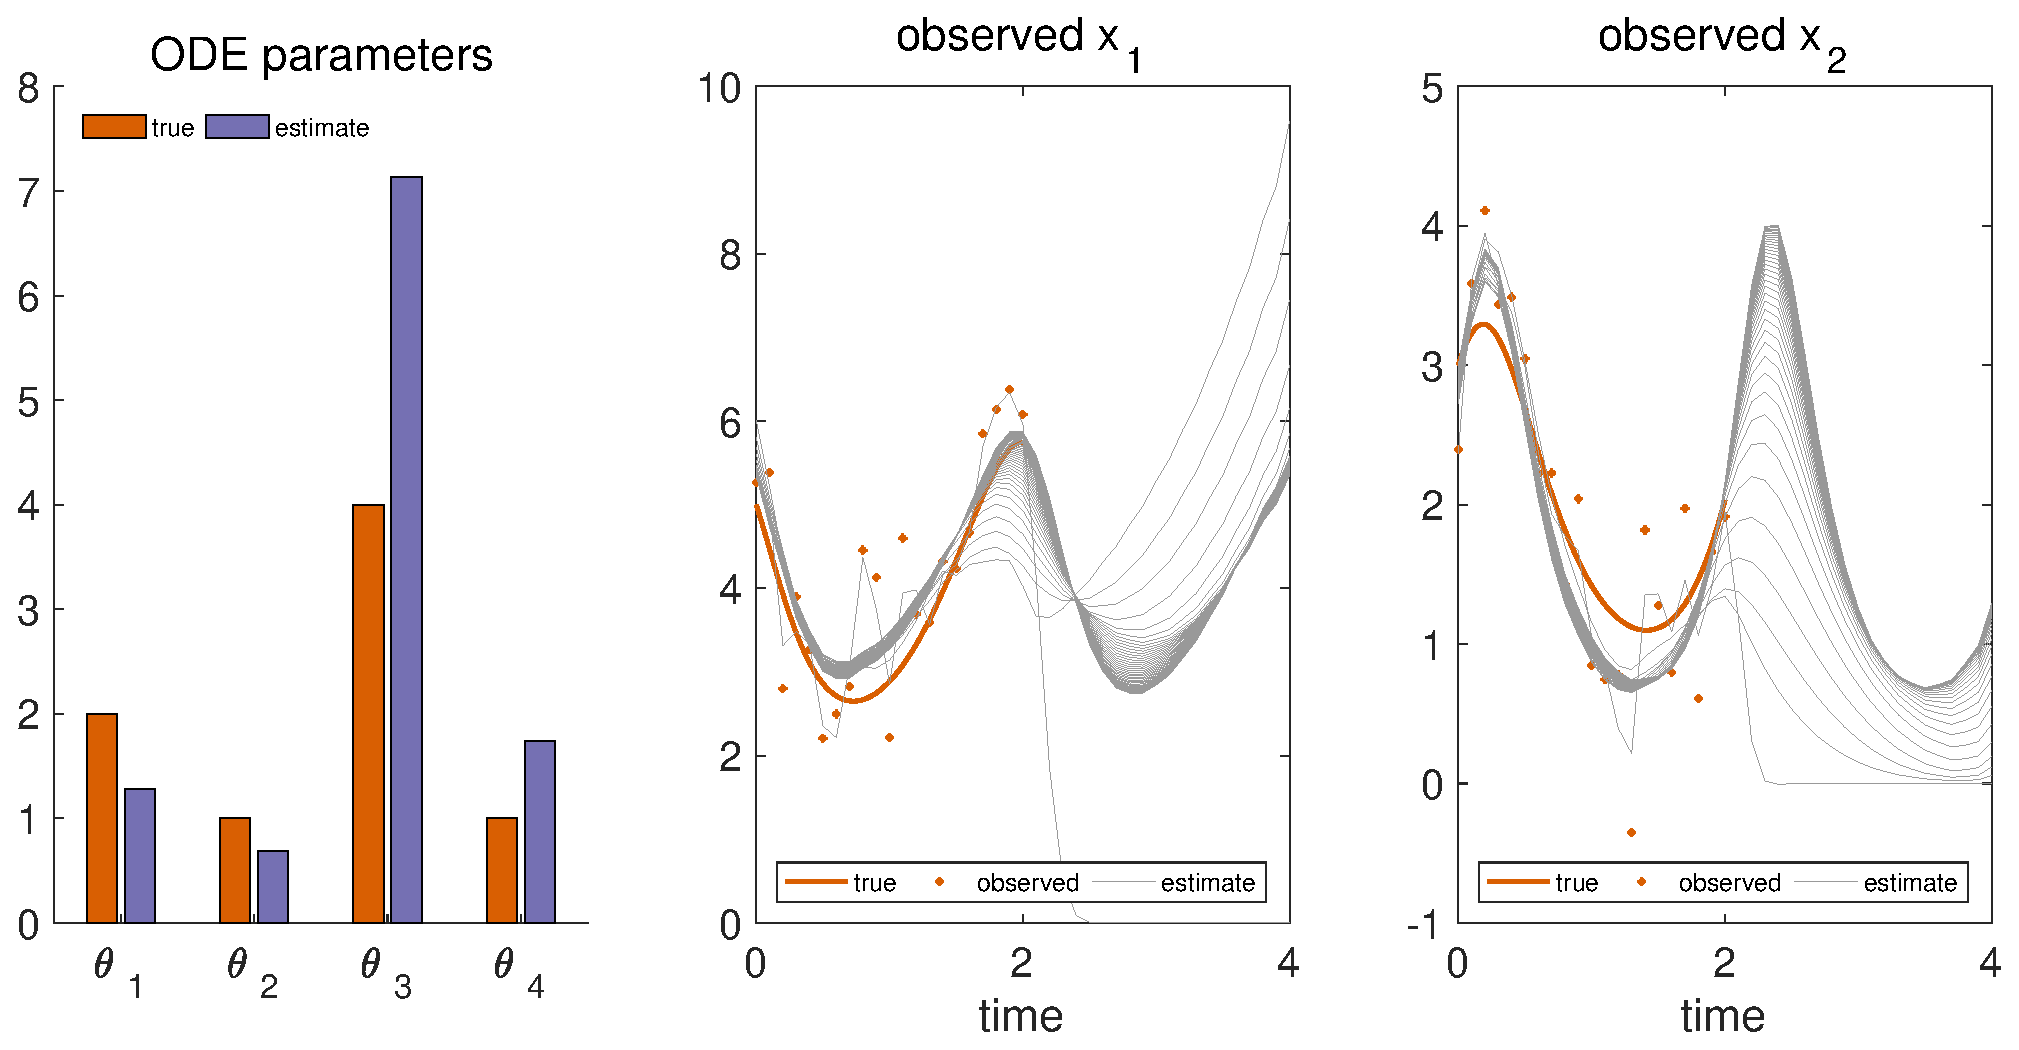
\includegraphics [width=5in]{VGM_for_Lotka_Volterra_40.eps}

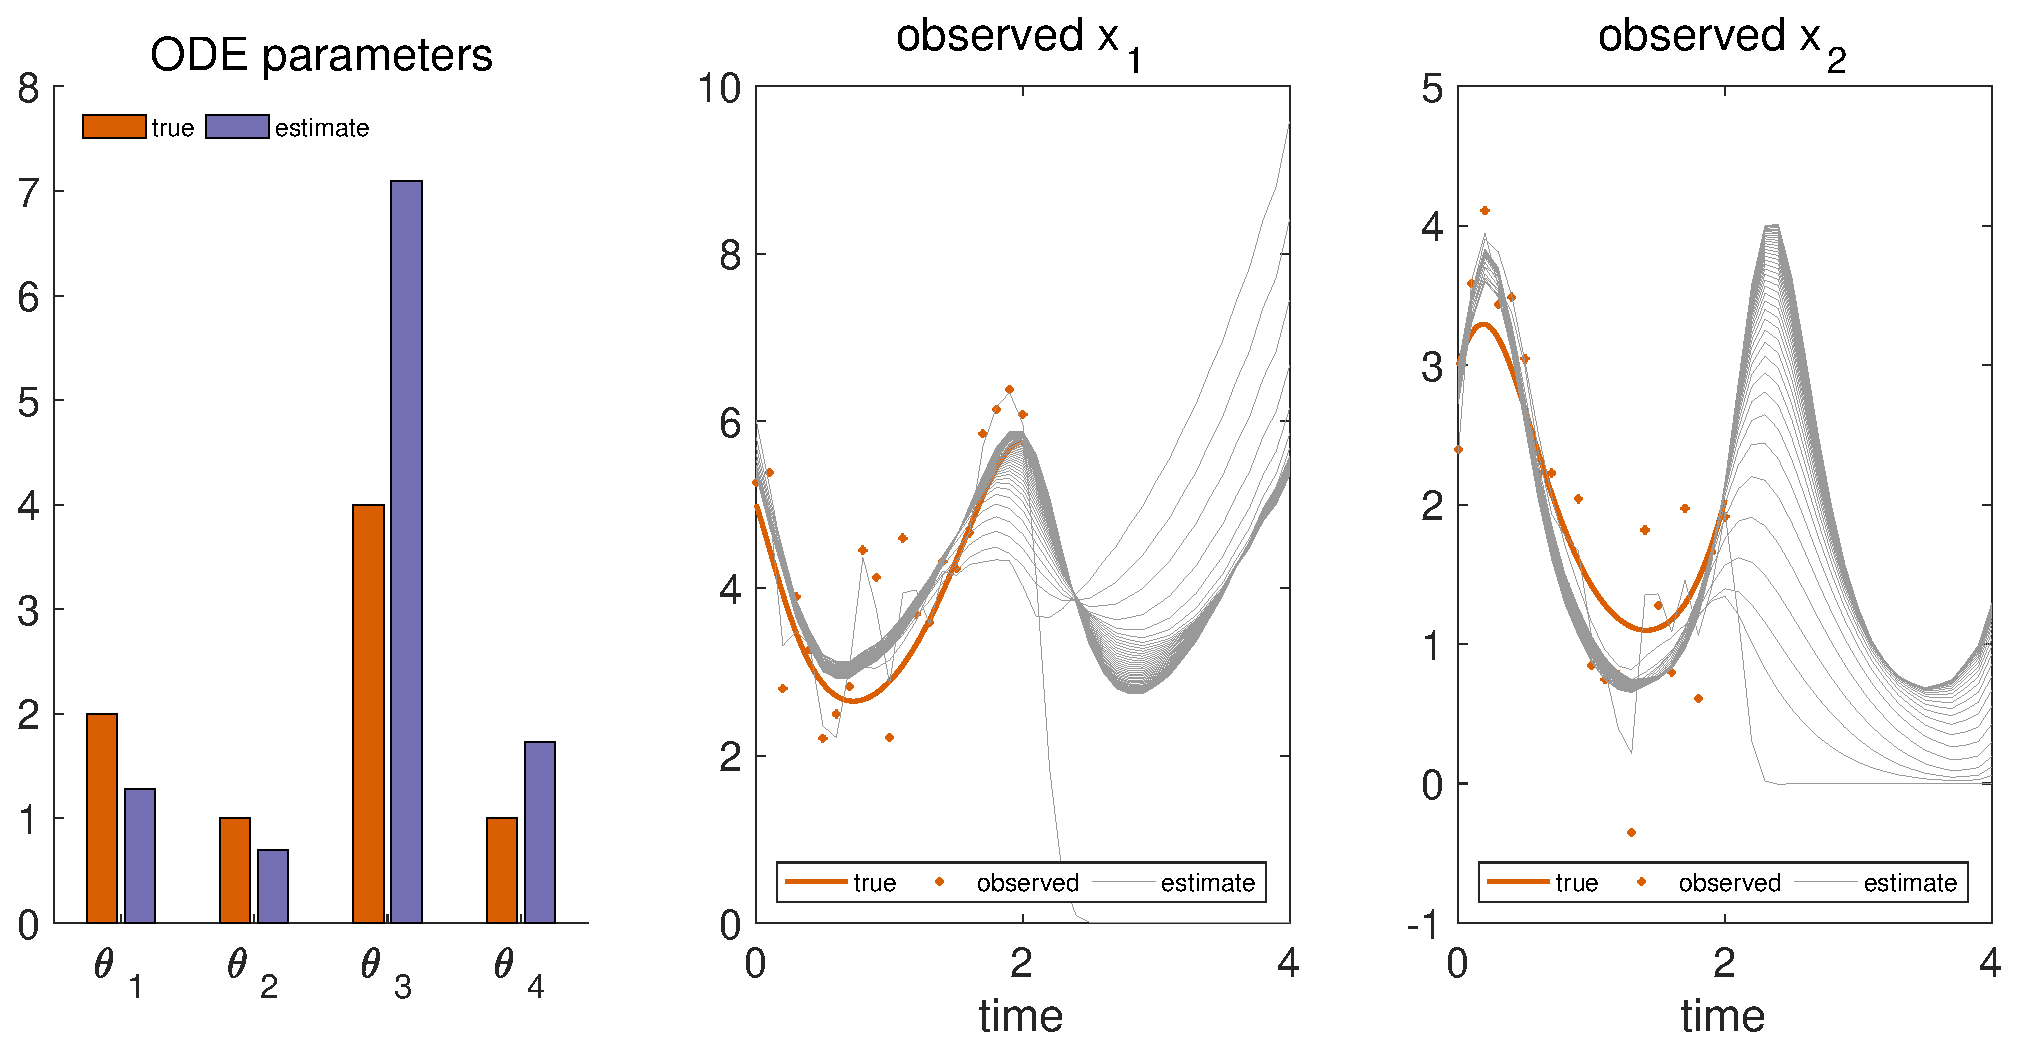
\includegraphics [width=5in]{VGM_for_Lotka_Volterra_41.eps}

}
\begin{par}

\end{par} \vspace{1em}
\subsection{Proxy for individual states}


Expanding the proxy distribution in equation (12) over the individual state $\mathbf{x}_u$:
\vspace{1em}
    
$\hat{q}(\mathbf{x}_u) \stackrel{(a)}{\propto} \exp \left(
~ E_{Q_{-u}}  \ln ( p(\mathbf{x}_u \mid \boldsymbol\theta, \mathbf{X}_{-u},\boldsymbol\phi,\gamma)
p(\mathbf{x}_u  \mid\mathbf{Y},\boldsymbol\phi,\boldsymbol\sigma) ) ~ \right)\\ \qquad
~ \stackrel{(b)}{=} \exp\big( ~ E_{Q_{-u}} \ln     \mathcal{N}\left(\mathbf{x}_u
; -\mathbf{B}_{u}^+ \mathbf{b}_u,     ~\mathbf{B}_u^{+} ~ (\mathbf{A} + \mathbf{I}\gamma)
~     \mathbf{B}_u^{+T} \right) + E_{Q_{-u}} \ln    \mathcal{N}\left(\mathbf{x}_u
; \boldsymbol\mu_u(\mathbf{Y}), \boldsymbol\Sigma_u    \right) \big)\\ \qquad ~= \exp\big(
~ E_{Q_{-u}} \ln                \mathcal{N}\left(\mathbf{x}_u ; -\mathbf{B}_{u}^+
\mathbf{b}_u,                ~\mathbf{B}_u^{+} ~ (\mathbf{A} + \mathbf{I}\gamma)
~                \mathbf{B}_u^{+T} \right) + E_{Q_{-u}} \ln                \mathcal{N}\left(\mathbf{x}_u
; \boldsymbol\mu_u(\mathbf{Y}), \boldsymbol{\sigma}_u                \right) \big)$.
    
In (a) we decompose the full conditional into an ODE-informed
distribution and a data-informed distribution and in (b) we substitute the ODE-informed
distribution $p(\mathbf{x}_u \mid \boldsymbol\theta, \mathbf{X}_{-u},\boldsymbol\phi,\gamma)$
with its density given by equation (8).
    \color{RoyalPurple}\begin{verbatim}
            [state.proxy.mean{:,symbols.state_string},state.proxy.inv_cov] = ...
            proxy_for_ind_states(state.lin_comb,...
            state.proxy.mean{:,symbols.state_string},...
            param_proxy_mean',dC_times_invC,coupling_idx.states,...
            symbols,mu,inv_sigma,simulation.observed_states,...
            A_plus_gamma_inv,opt_settings);
\end{verbatim}
\color{black}
\color{RoyalPurple}\begin{verbatim}
end
\end{verbatim}
\color{black}
\begin{par}

\end{par} \vspace{1em}
\begin{par}
Final results
\end{par} \vspace{1em}
\color{RoyalPurple}\begin{verbatim}
plot_results(fig_handle,state.proxy,simulation,param_proxy_mean,...
   plot_handle,symbols,plot_settings,'final');
\end{verbatim}
\color{black}

{
\centering
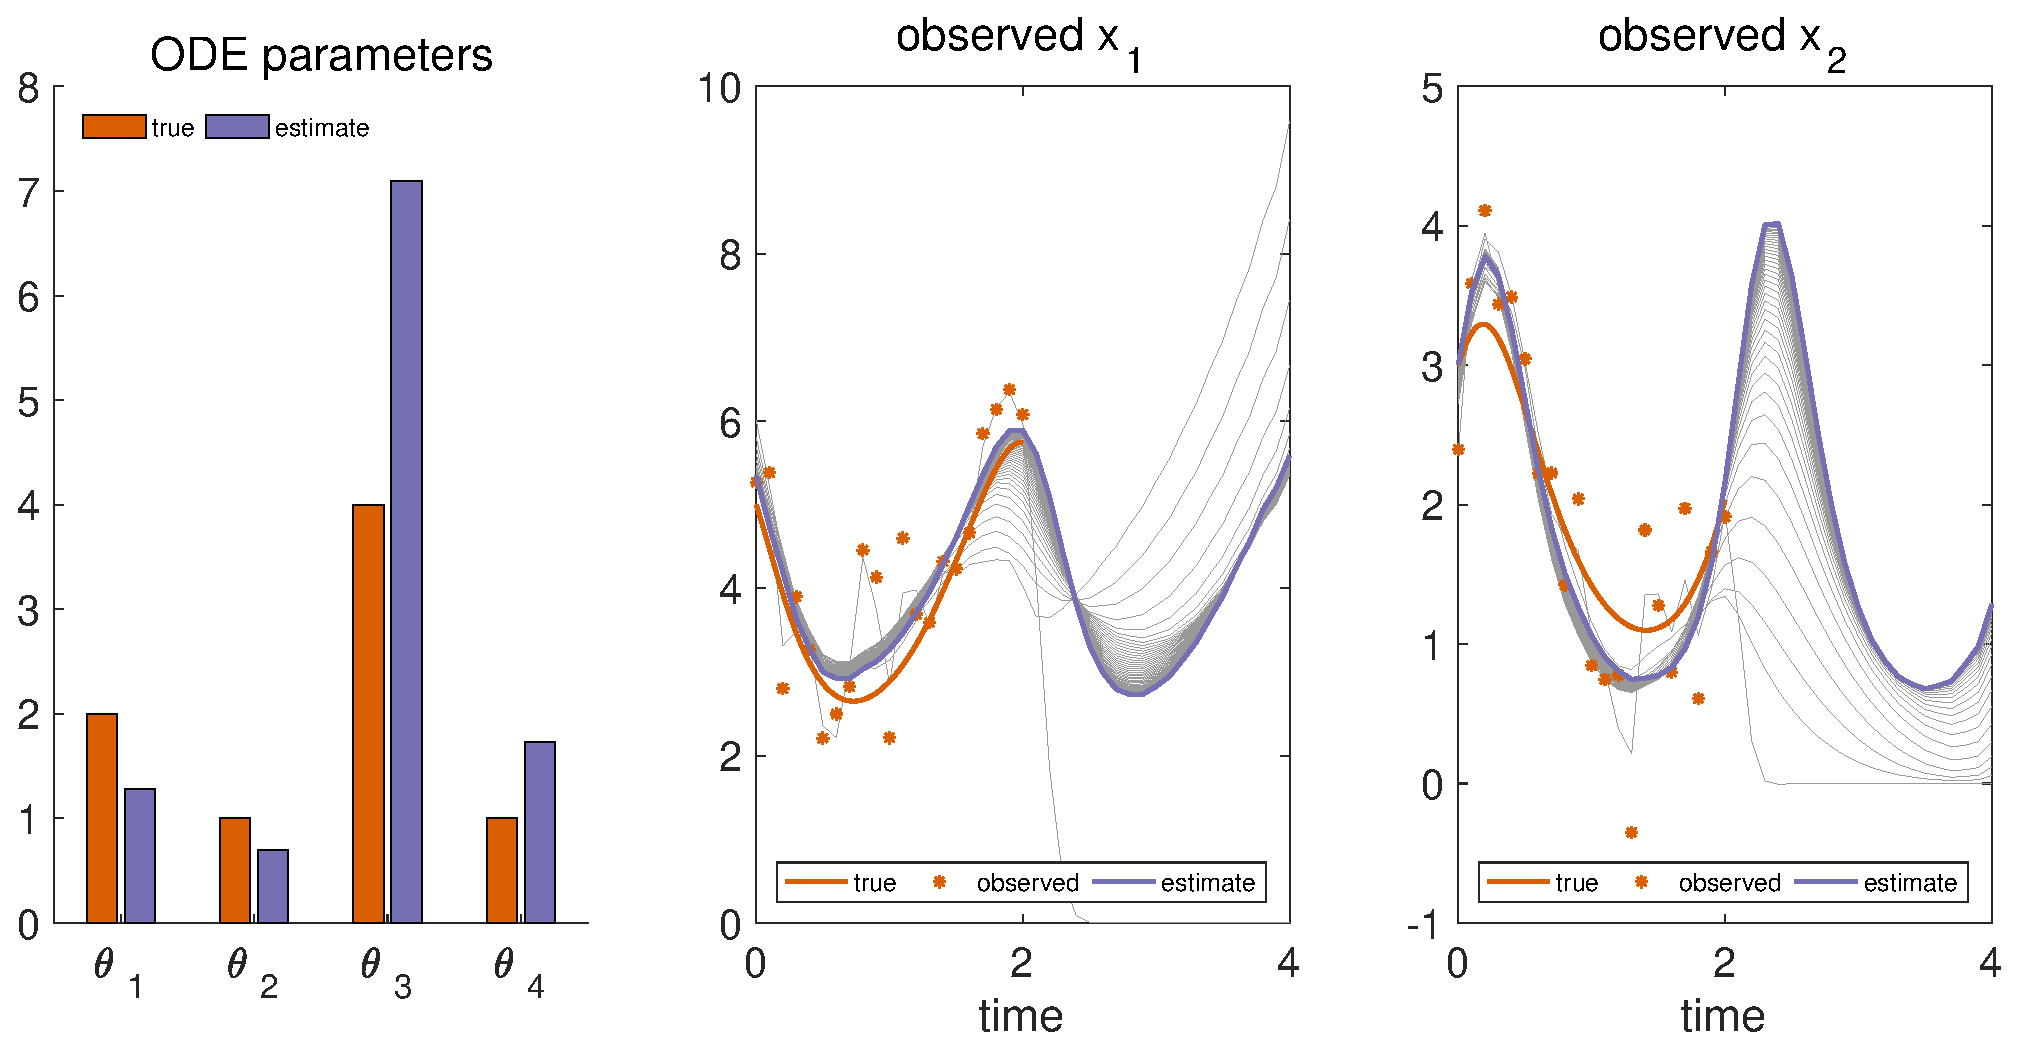
\includegraphics [width=5in]{VGM_for_Lotka_Volterra_42.eps}

}

\section{Time Taken}

\color{RoyalPurple}\begin{verbatim}
disp(['time taken: ' num2str(toc) ' seconds'])
\end{verbatim}
\color{black}
\color{black}

        \color{MidnightBlue}\begin{verbatim}time taken: 44.1589 seconds
\end{verbatim}
\color{black} 
\cleardoublepage

  \setcounter{chapter}{2}
  \setcounter{section}{0}
\chapter*{VGM for Lorenz 96}   
\phantomsection\addcontentsline{toc}{chapter}{VGM for Lorenz 96}
\section{Simulation Settings}

\color{RoyalPurple}\begin{verbatim}
simulation.numb_odes = 100;          % number of ODEs
% observation noise
simulation.state_obs_variance = @(mean)(bsxfun(@times,0.1,ones(size(mean))));
simulation.ode_param = 8;            % true ODE parameter;
simulation.final_time = 4;           % end time for integration
simulation.int_interval = 0.01;      % integration interval
simulation.time_samp = 0:0.125:simulation.final_time; % sample times for observations
simulation.init_val = zeros(1,simulation.numb_odes); % initial state values

% ratio of number of observed states over number of unobserved states.
simulation.observed_states = 0.5;    % only 50% of the states are observed
\end{verbatim}
\color{black}


\section{User Input}

\begin{par}
\subsection{ Path to ODEs }
\end{par} \vspace{1em}
\color{RoyalPurple}\begin{verbatim}
odes_path = 'Lorenz96_ODEs.txt';
\end{verbatim}
\color{black}
\begin{par}
\subsection{ Symbols } symbols of states and parameters in the '\_ODEs.txt' file
\end{par} \vspace{1em}
\begin{par}
States $\mathbf{x}$:
\end{par} \vspace{1em}
\color{RoyalPurple}\begin{verbatim}
for u = 1:simulation.numb_odes; symbols.state(u) = {['[x_' num2str(u) ']']}; end
\end{verbatim}
\color{black}
\begin{par}
ODE parameters $\theta$ (symbols of parameters in 'ODEs.txt' file):
\end{par} \vspace{1em}
\color{RoyalPurple}\begin{verbatim}
symbols.param = {'[\theta]'};
% \section{ Kernel }
%
% Kernel parameters $\phi$:
kernel.param = [10,0.2];             % set values of rbf kernel parameters
\end{verbatim}
\color{black}
\begin{par}
Error variance on state derivatives (i.e. $\gamma$):
\end{par} \vspace{1em}
\color{RoyalPurple}\begin{verbatim}
state.derivative_variance = 6*ones(1,length(symbols.state)); % gamma for gradient matching model
\end{verbatim}
\color{black}
\begin{par}
\subsection{ Estimation times }
\end{par} \vspace{1em}
\color{RoyalPurple}\begin{verbatim}
time.est = 0:0.1:4;                 % estimation times
\end{verbatim}
\color{black}
\begin{par}
\subsection{ Type of pseudo-inverse } Type of pseudo inverse; options: 'Moore-Penrose' or 'modified Moore-Penrose'
\end{par} \vspace{1em}
\color{RoyalPurple}\begin{verbatim}
opt_settings.pseudo_inv_type = 'Moore-Penrose';
\end{verbatim}
\color{black}
\begin{par}
\subsection{ Optimization settings }
\end{par} \vspace{1em}
\color{RoyalPurple}\begin{verbatim}
opt_settings.coord_ascent_numb_iter = 10;  % number of coordinate ascent iterations

% The observed state trajectories are clamped to the trajectories
% determined by standard GP regression (Boolean)
opt_settings.clamp_obs_state_to_GP_fit = true;
\end{verbatim}
\color{black}
\begin{par}
Plot settings: layout and size
\end{par} \vspace{1em}
\color{RoyalPurple}\begin{verbatim}
plot_settings.size = [1600, 800]; plot_settings.layout = [3,3];
\end{verbatim}
\color{black}


\section{Import ODEs}

\color{RoyalPurple}\begin{verbatim}
generate_Lorenz96_ODEs(simulation.numb_odes)
ode = import_odes(symbols,odes_path);
\end{verbatim}
\color{black}
\color{RoyalPurple}\begin{verbatim}
disp('ODEs:'); disp(ode.raw)
\end{verbatim}
\color{black}

        \begin{verbatim}ODEs:
    '([x_2] - [x_99]) .* [x_100] - [x_1] + [\theta]'
    '([x_3] - [x_100]) .* [x_1] - [x_2] + [\theta]'
    '([x_4] - [x_1]) .* [x_2] - [x_3] + [\theta]'
    '([x_5] - [x_2]) .* [x_3] - [x_4] + [\theta]'
    '([x_6] - [x_3]) .* [x_4] - [x_5] + [\theta]'
    '([x_7] - [x_4]) .* [x_5] - [x_6] + [\theta]'
    '([x_8] - [x_5]) .* [x_6] - [x_7] + [\theta]'
    '([x_9] - [x_6]) .* [x_7] - [x_8] + [\theta]'
    '([x_10] - [x_7]) .* [x_8] - [x_9] + [\theta]'
    '([x_11] - [x_8]) .* [x_9] - [x_10] + [\theta]'
    '([x_12] - [x_9]) .* [x_10] - [x_11] + [\theta]'
    '([x_13] - [x_10]) .* [x_11] - [x_12] + [\theta]'
    '([x_14] - [x_11]) .* [x_12] - [x_13] + [\theta]'
    '([x_15] - [x_12]) .* [x_13] - [x_14] + [\theta]'
    '([x_16] - [x_13]) .* [x_14] - [x_15] + [\theta]'
    '([x_17] - [x_14]) .* [x_15] - [x_16] + [\theta]'
    '([x_18] - [x_15]) .* [x_16] - [x_17] + [\theta]'
    '([x_19] - [x_16]) .* [x_17] - [x_18] + [\theta]'
    '([x_20] - [x_17]) .* [x_18] - [x_19] + [\theta]'
    '([x_21] - [x_18]) .* [x_19] - [x_20] + [\theta]'
    '([x_22] - [x_19]) .* [x_20] - [x_21] + [\theta]'
    '([x_23] - [x_20]) .* [x_21] - [x_22] + [\theta]'
    '([x_24] - [x_21]) .* [x_22] - [x_23] + [\theta]'
    '([x_25] - [x_22]) .* [x_23] - [x_24] + [\theta]'
    '([x_26] - [x_23]) .* [x_24] - [x_25] + [\theta]'
    '([x_27] - [x_24]) .* [x_25] - [x_26] + [\theta]'
    '([x_28] - [x_25]) .* [x_26] - [x_27] + [\theta]'
    '([x_29] - [x_26]) .* [x_27] - [x_28] + [\theta]'
    '([x_30] - [x_27]) .* [x_28] - [x_29] + [\theta]'
    '([x_31] - [x_28]) .* [x_29] - [x_30] + [\theta]'
    '([x_32] - [x_29]) .* [x_30] - [x_31] + [\theta]'
    '([x_33] - [x_30]) .* [x_31] - [x_32] + [\theta]'
    '([x_34] - [x_31]) .* [x_32] - [x_33] + [\theta]'
    '([x_35] - [x_32]) .* [x_33] - [x_34] + [\theta]'
    '([x_36] - [x_33]) .* [x_34] - [x_35] + [\theta]'
    '([x_37] - [x_34]) .* [x_35] - [x_36] + [\theta]'
    '([x_38] - [x_35]) .* [x_36] - [x_37] + [\theta]'
    '([x_39] - [x_36]) .* [x_37] - [x_38] + [\theta]'
    '([x_40] - [x_37]) .* [x_38] - [x_39] + [\theta]'
    '([x_41] - [x_38]) .* [x_39] - [x_40] + [\theta]'
    '([x_42] - [x_39]) .* [x_40] - [x_41] + [\theta]'
    '([x_43] - [x_40]) .* [x_41] - [x_42] + [\theta]'
    '([x_44] - [x_41]) .* [x_42] - [x_43] + [\theta]'
    '([x_45] - [x_42]) .* [x_43] - [x_44] + [\theta]'
    '([x_46] - [x_43]) .* [x_44] - [x_45] + [\theta]'
    '([x_47] - [x_44]) .* [x_45] - [x_46] + [\theta]'
    '([x_48] - [x_45]) .* [x_46] - [x_47] + [\theta]'
    '([x_49] - [x_46]) .* [x_47] - [x_48] + [\theta]'
    '([x_50] - [x_47]) .* [x_48] - [x_49] + [\theta]'
    '([x_51] - [x_48]) .* [x_49] - [x_50] + [\theta]'
    '([x_52] - [x_49]) .* [x_50] - [x_51] + [\theta]'
    '([x_53] - [x_50]) .* [x_51] - [x_52] + [\theta]'
    '([x_54] - [x_51]) .* [x_52] - [x_53] + [\theta]'
    '([x_55] - [x_52]) .* [x_53] - [x_54] + [\theta]'
    '([x_56] - [x_53]) .* [x_54] - [x_55] + [\theta]'
    '([x_57] - [x_54]) .* [x_55] - [x_56] + [\theta]'
    '([x_58] - [x_55]) .* [x_56] - [x_57] + [\theta]'
    '([x_59] - [x_56]) .* [x_57] - [x_58] + [\theta]'
    '([x_60] - [x_57]) .* [x_58] - [x_59] + [\theta]'
    '([x_61] - [x_58]) .* [x_59] - [x_60] + [\theta]'
    '([x_62] - [x_59]) .* [x_60] - [x_61] + [\theta]'
    '([x_63] - [x_60]) .* [x_61] - [x_62] + [\theta]'
    '([x_64] - [x_61]) .* [x_62] - [x_63] + [\theta]'
    '([x_65] - [x_62]) .* [x_63] - [x_64] + [\theta]'
    '([x_66] - [x_63]) .* [x_64] - [x_65] + [\theta]'
    '([x_67] - [x_64]) .* [x_65] - [x_66] + [\theta]'
    '([x_68] - [x_65]) .* [x_66] - [x_67] + [\theta]'
    '([x_69] - [x_66]) .* [x_67] - [x_68] + [\theta]'
    '([x_70] - [x_67]) .* [x_68] - [x_69] + [\theta]'
    '([x_71] - [x_68]) .* [x_69] - [x_70] + [\theta]'
    '([x_72] - [x_69]) .* [x_70] - [x_71] + [\theta]'
    '([x_73] - [x_70]) .* [x_71] - [x_72] + [\theta]'
    '([x_74] - [x_71]) .* [x_72] - [x_73] + [\theta]'
    '([x_75] - [x_72]) .* [x_73] - [x_74] + [\theta]'
    '([x_76] - [x_73]) .* [x_74] - [x_75] + [\theta]'
    '([x_77] - [x_74]) .* [x_75] - [x_76] + [\theta]'
    '([x_78] - [x_75]) .* [x_76] - [x_77] + [\theta]'
    '([x_79] - [x_76]) .* [x_77] - [x_78] + [\theta]'
    '([x_80] - [x_77]) .* [x_78] - [x_79] + [\theta]'
    '([x_81] - [x_78]) .* [x_79] - [x_80] + [\theta]'
    '([x_82] - [x_79]) .* [x_80] - [x_81] + [\theta]'
    '([x_83] - [x_80]) .* [x_81] - [x_82] + [\theta]'
    '([x_84] - [x_81]) .* [x_82] - [x_83] + [\theta]'
    '([x_85] - [x_82]) .* [x_83] - [x_84] + [\theta]'
    '([x_86] - [x_83]) .* [x_84] - [x_85] + [\theta]'
    '([x_87] - [x_84]) .* [x_85] - [x_86] + [\theta]'
    '([x_88] - [x_85]) .* [x_86] - [x_87] + [\theta]'
    '([x_89] - [x_86]) .* [x_87] - [x_88] + [\theta]'
    '([x_90] - [x_87]) .* [x_88] - [x_89] + [\theta]'
    '([x_91] - [x_88]) .* [x_89] - [x_90] + [\theta]'
    '([x_92] - [x_89]) .* [x_90] - [x_91] + [\theta]'
    '([x_93] - [x_90]) .* [x_91] - [x_92] + [\theta]'
    '([x_94] - [x_91]) .* [x_92] - [x_93] + [\theta]'
    '([x_95] - [x_92]) .* [x_93] - [x_94] + [\theta]'
    '([x_96] - [x_93]) .* [x_94] - [x_95] + [\theta]'
    '([x_97] - [x_94]) .* [x_95] - [x_96] + [\theta]'
    '([x_98] - [x_95]) .* [x_96] - [x_97] + [\theta]'
    '([x_99] - [x_96]) .* [x_97] - [x_98] + [\theta]'
    '([x_100] - [x_97]) .* [x_98] - [x_99] + [\theta]'
    '([x_1] - [x_98]) .* [x_99] - [x_100] + [\theta]'

\end{verbatim}
\color{black}
    

\section{Simulate Trajectory Observations}

\begin{par}
\subsection{ Generate ground truth by numerical integration }
\end{par} \vspace{1em}
\color{RoyalPurple}\begin{verbatim}
[state,time,ode] = generate_ground_truth(time,state,ode,symbols,simulation,...
    odes_path);
\end{verbatim}
\color{black}
\begin{par}
\subsection{ Generate state observations }
\end{par} \vspace{1em}
\color{RoyalPurple}\begin{verbatim}
if ~iscell(simulation.observed_states)
    ratio_observed = simulation.observed_states;
    state_obs_idx = zeros(1,simulation.numb_odes,'logical');
    idx = randperm(simulation.numb_odes);
    idx = idx(1:floor(simulation.numb_odes * ratio_observed));
    state_obs_idx(idx) = 1;
    simulation.observed_states = symbols.state(state_obs_idx);
end

[state,time,obs_to_state_relation] = generate_state_obs(state,time,simulation,...
    symbols);
\end{verbatim}
\color{black}
\begin{par}
\subsection{ Symbols }
\end{par} \vspace{1em}
\color{RoyalPurple}\begin{verbatim}
state.sym.mean = sym('x%d%d',[length(time.est),length(ode.system)]);
state.sym.variance = sym('sigma%d%d',[length(time.est),length(ode.system)]);
ode_param.sym.mean = sym('param%d',[length(symbols.param),1]);
assume(ode_param.sym.mean,'real');
\end{verbatim}
\color{black}
\begin{par}
\subsection{ Setup plots }
\end{par} \vspace{1em}
\begin{par}
Only the state dynamics are (partially) observed.
\end{par} \vspace{1em}
\color{RoyalPurple}\begin{verbatim}
[h_states,h_param,p] = setup_plots(state,time,simulation,symbols,plot_settings);

tic; %start timer
\end{verbatim}
\color{black}

\color{RoyalPurple}\begin{verbatim}
[dC_times_invC,inv_C,A_plus_gamma_inv] = kernel_function(kernel,state,time.est);
\end{verbatim}
\color{black}


\section{State Couplings in ODEs}

\color{RoyalPurple}\begin{verbatim}
coupling_idx = find_state_couplings_in_odes(ode,symbols);
\end{verbatim}
\color{black}

\section{Prior over State and State Derivatives}
\color{RoyalPurple}\begin{verbatim}
[dC_times_invC,inv_C,A_plus_gamma_inv] = kernel_function(kernel,state,time.est);
\end{verbatim}
\color{black}

\section{Rewrite ODEs as Linear Combination in Parameters}

\begin{par}
We rewrite the ODEs in equation (2) as a linear combination in the parameters:
\end{par} \vspace{1em}
\begin{par}
$\mathbf{B}_{\theta k} \theta + \mathbf{b}_{\theta k} \stackrel{!}{=} \mathbf{f}_k(\mathbf{X},\theta) \qquad (5)$,
\end{par} \vspace{1em}
\begin{par}
where matrices $\mathbf{B}_{\theta k}$ and $\mathbf{b}_{\theta k}$ are defined such that the ODEs $\mathbf{f}_k(\mathbf{X},\theta)$ are expressed as a linear combination in $\theta$.
\end{par} \vspace{1em}
\color{RoyalPurple}\begin{verbatim}
[ode_param.lin_comb.B,ode_param.lin_comb.b] = ...
    rewrite_odes_as_linear_combination_in_parameters(ode,symbols);
\end{verbatim}
\color{black}


\section{Rewrite ODEs as Linear Combination in Individual States}

\begin{par}
We rewrite the expression $\mathbf{f}(\mathbf{X},\theta) - {'\mathbf{C}}_{\phi} \mathbf{C}_{\phi}^{-1} \mathbf{X}$ in equation (4) as a linear combination in the individual state $\mathbf{x}_u$:
\end{par} \vspace{1em}
\begin{par}
$\mathbf{R}_{uk} \mathbf{x}_u + \mathbf{r}_{uk} \stackrel{!}{=} \mathbf{f}_k(\mathbf{X},\theta)$.
\end{par} \vspace{1em}
\begin{par}
where matrices $\mathbf{R}_{uk}$ and $\mathbf{r}_{uk}$ are defined such that the ODE $\mathbf{f}_k(\mathbf{X},\theta)$ is expressed as a linear combination in the individual state $\mathbf{x}_u$.
\end{par} \vspace{1em}
\color{RoyalPurple}\begin{verbatim}
[state.lin_comb.R,state.lin_comb.r] = ...
    rewrite_odes_as_linear_combination_in_ind_states(ode,symbols,coupling_idx.states);
\end{verbatim}
\color{black}

\section{Fitting observations of state trajectories}

\begin{par}
\color{RoyalPurple}\begin{verbatim}
[mu,inv_sigma] = fitting_state_observations(state,inv_C,obs_to_state_relation,simulation);
\end{verbatim}
\color{black}
\end{par}

\section{Coordinate Ascent Variational Gradient Matching}

\begin{par}
We minimize the KL-divergence in equation (10) by coordinate descent (where each step is analytically tractable) by iterating between determining the proxy for the distribution over ODE parameters $\hat{q}(\theta)$ and the proxies for the distribution over individual states $\hat{q}(\mathbf{x}_u)$.
\end{par} \vspace{1em}
\color{RoyalPurple}\begin{verbatim}
state.proxy.mean = mu;  % Initialize the state estimation by the GP regression posterior
for i = 1:opt_settings.coord_ascent_numb_iter
\end{verbatim}
\color{black}

\subsection{ Proxy for ODE parameters }
\color{RoyalPurple}\begin{verbatim}
    [param_proxy_mean,param_proxy_inv_cov] = proxy_for_ode_parameters(state.proxy.mean,...
        dC_times_invC,ode_param.lin_comb,symbols,A_plus_gamma_inv,opt_settings);

    if i==1 || ~mod(i,1)
        plot_results(h_states,h_param,state,time,simulation,param_proxy_mean,...
            p,symbols,'not_final');
    end
\end{verbatim}
\color{black}

\subsection{Proxy for individual states}
\color{RoyalPurple}\begin{verbatim}
    [state.proxy.mean,state.proxy.inv_cov] = proxy_for_ind_states(state.lin_comb,...
        state.proxy.mean,param_proxy_mean',dC_times_invC,coupling_idx.states,symbols,...
        mu,inv_sigma,simulation.observed_states,A_plus_gamma_inv,opt_settings);
\end{verbatim}

{
\centering
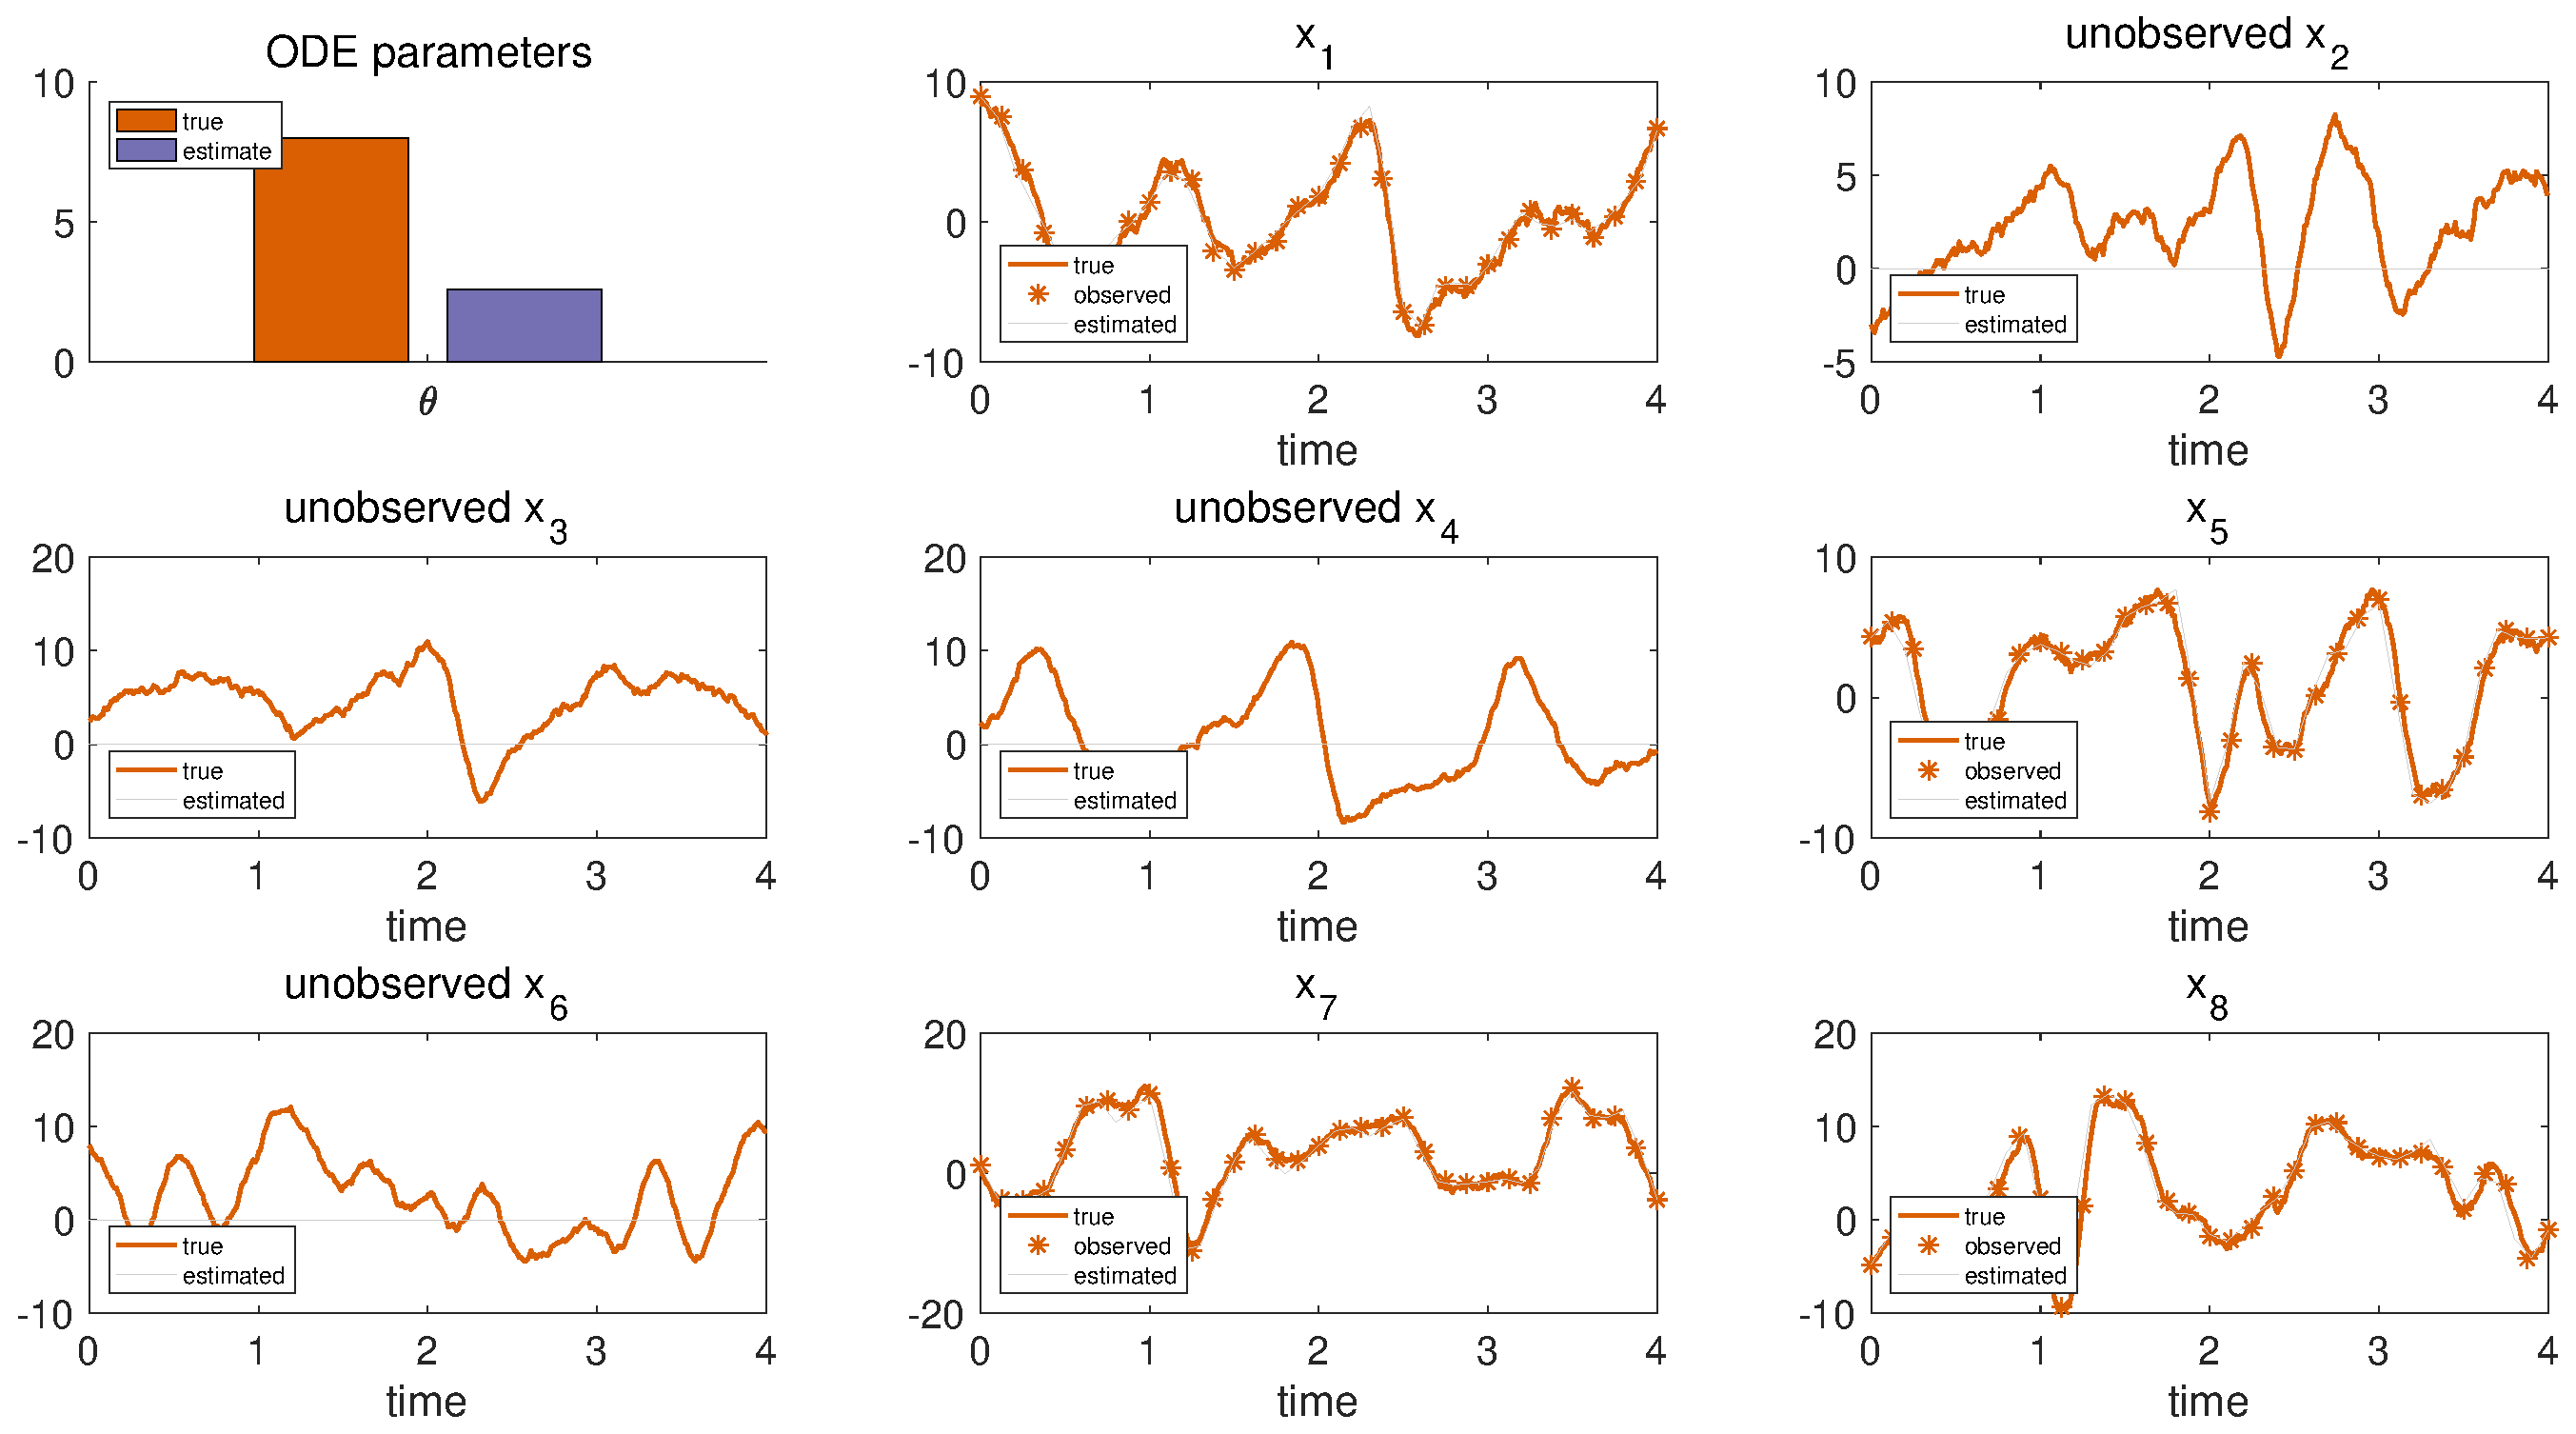
\includegraphics [width=5in]{Lorenz96_2_05.eps}

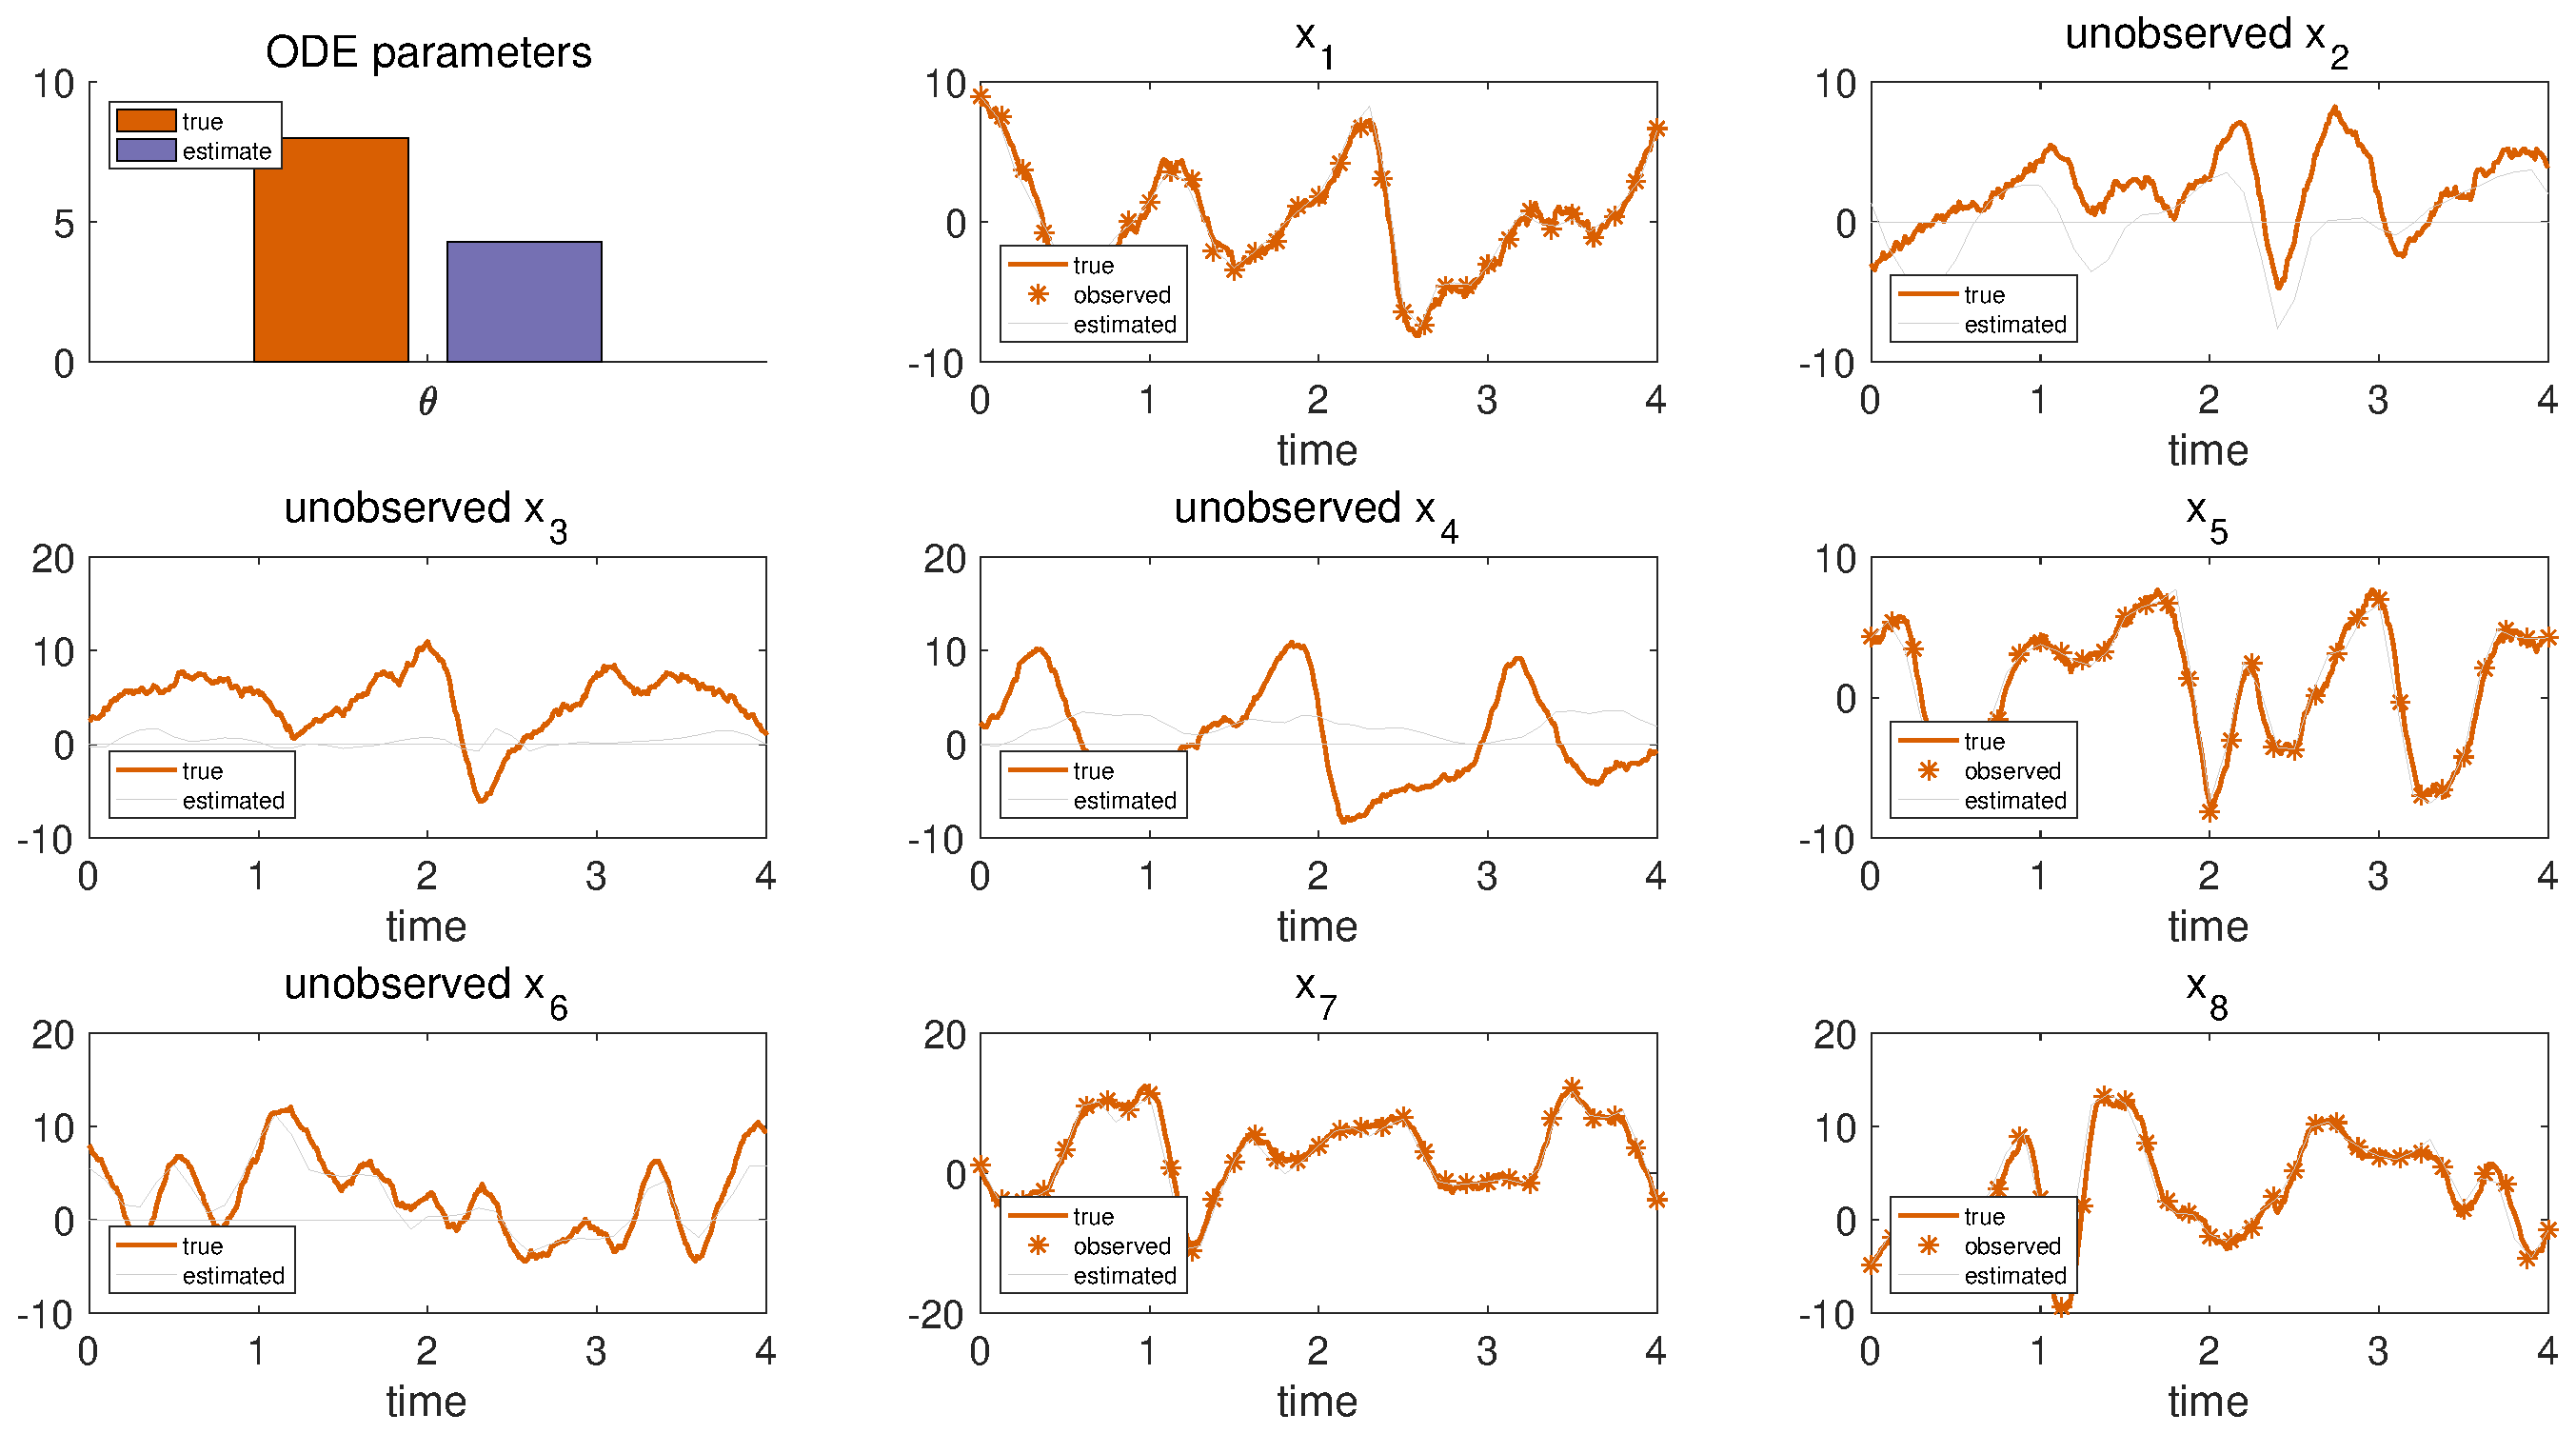
\includegraphics [width=5in]{Lorenz96_2_06.eps}

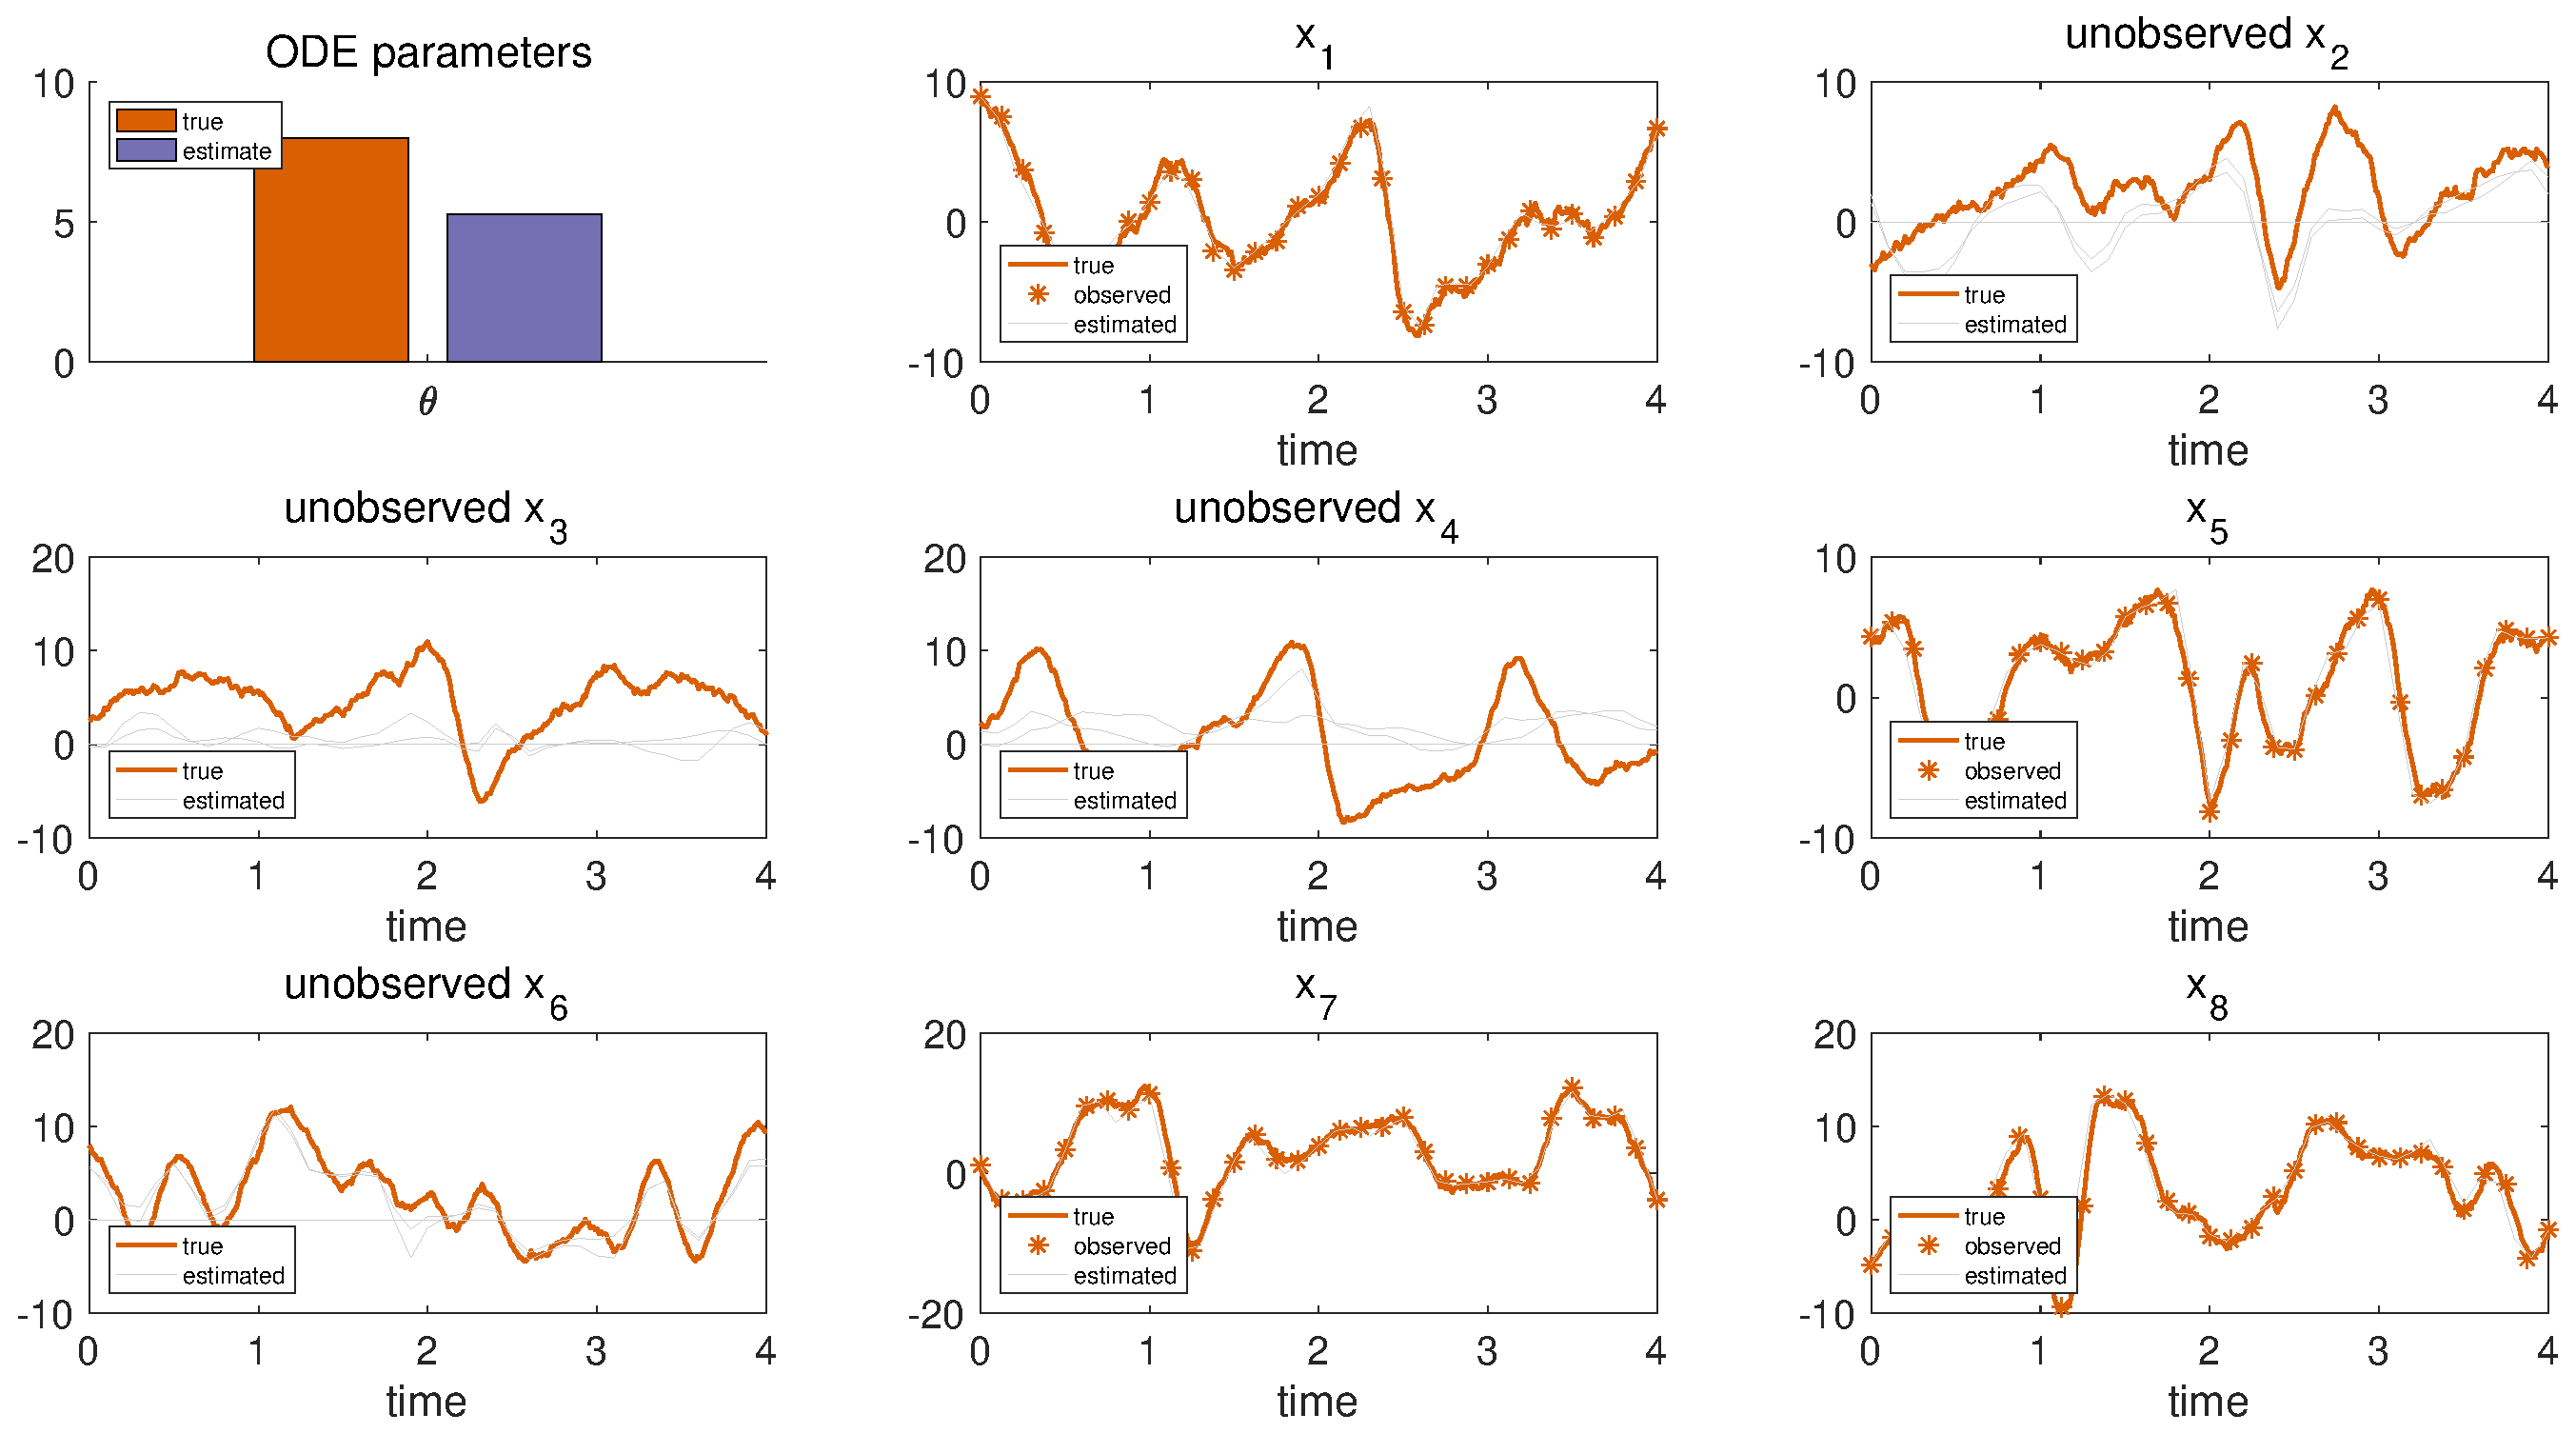
\includegraphics [width=5in]{Lorenz96_2_07.eps}

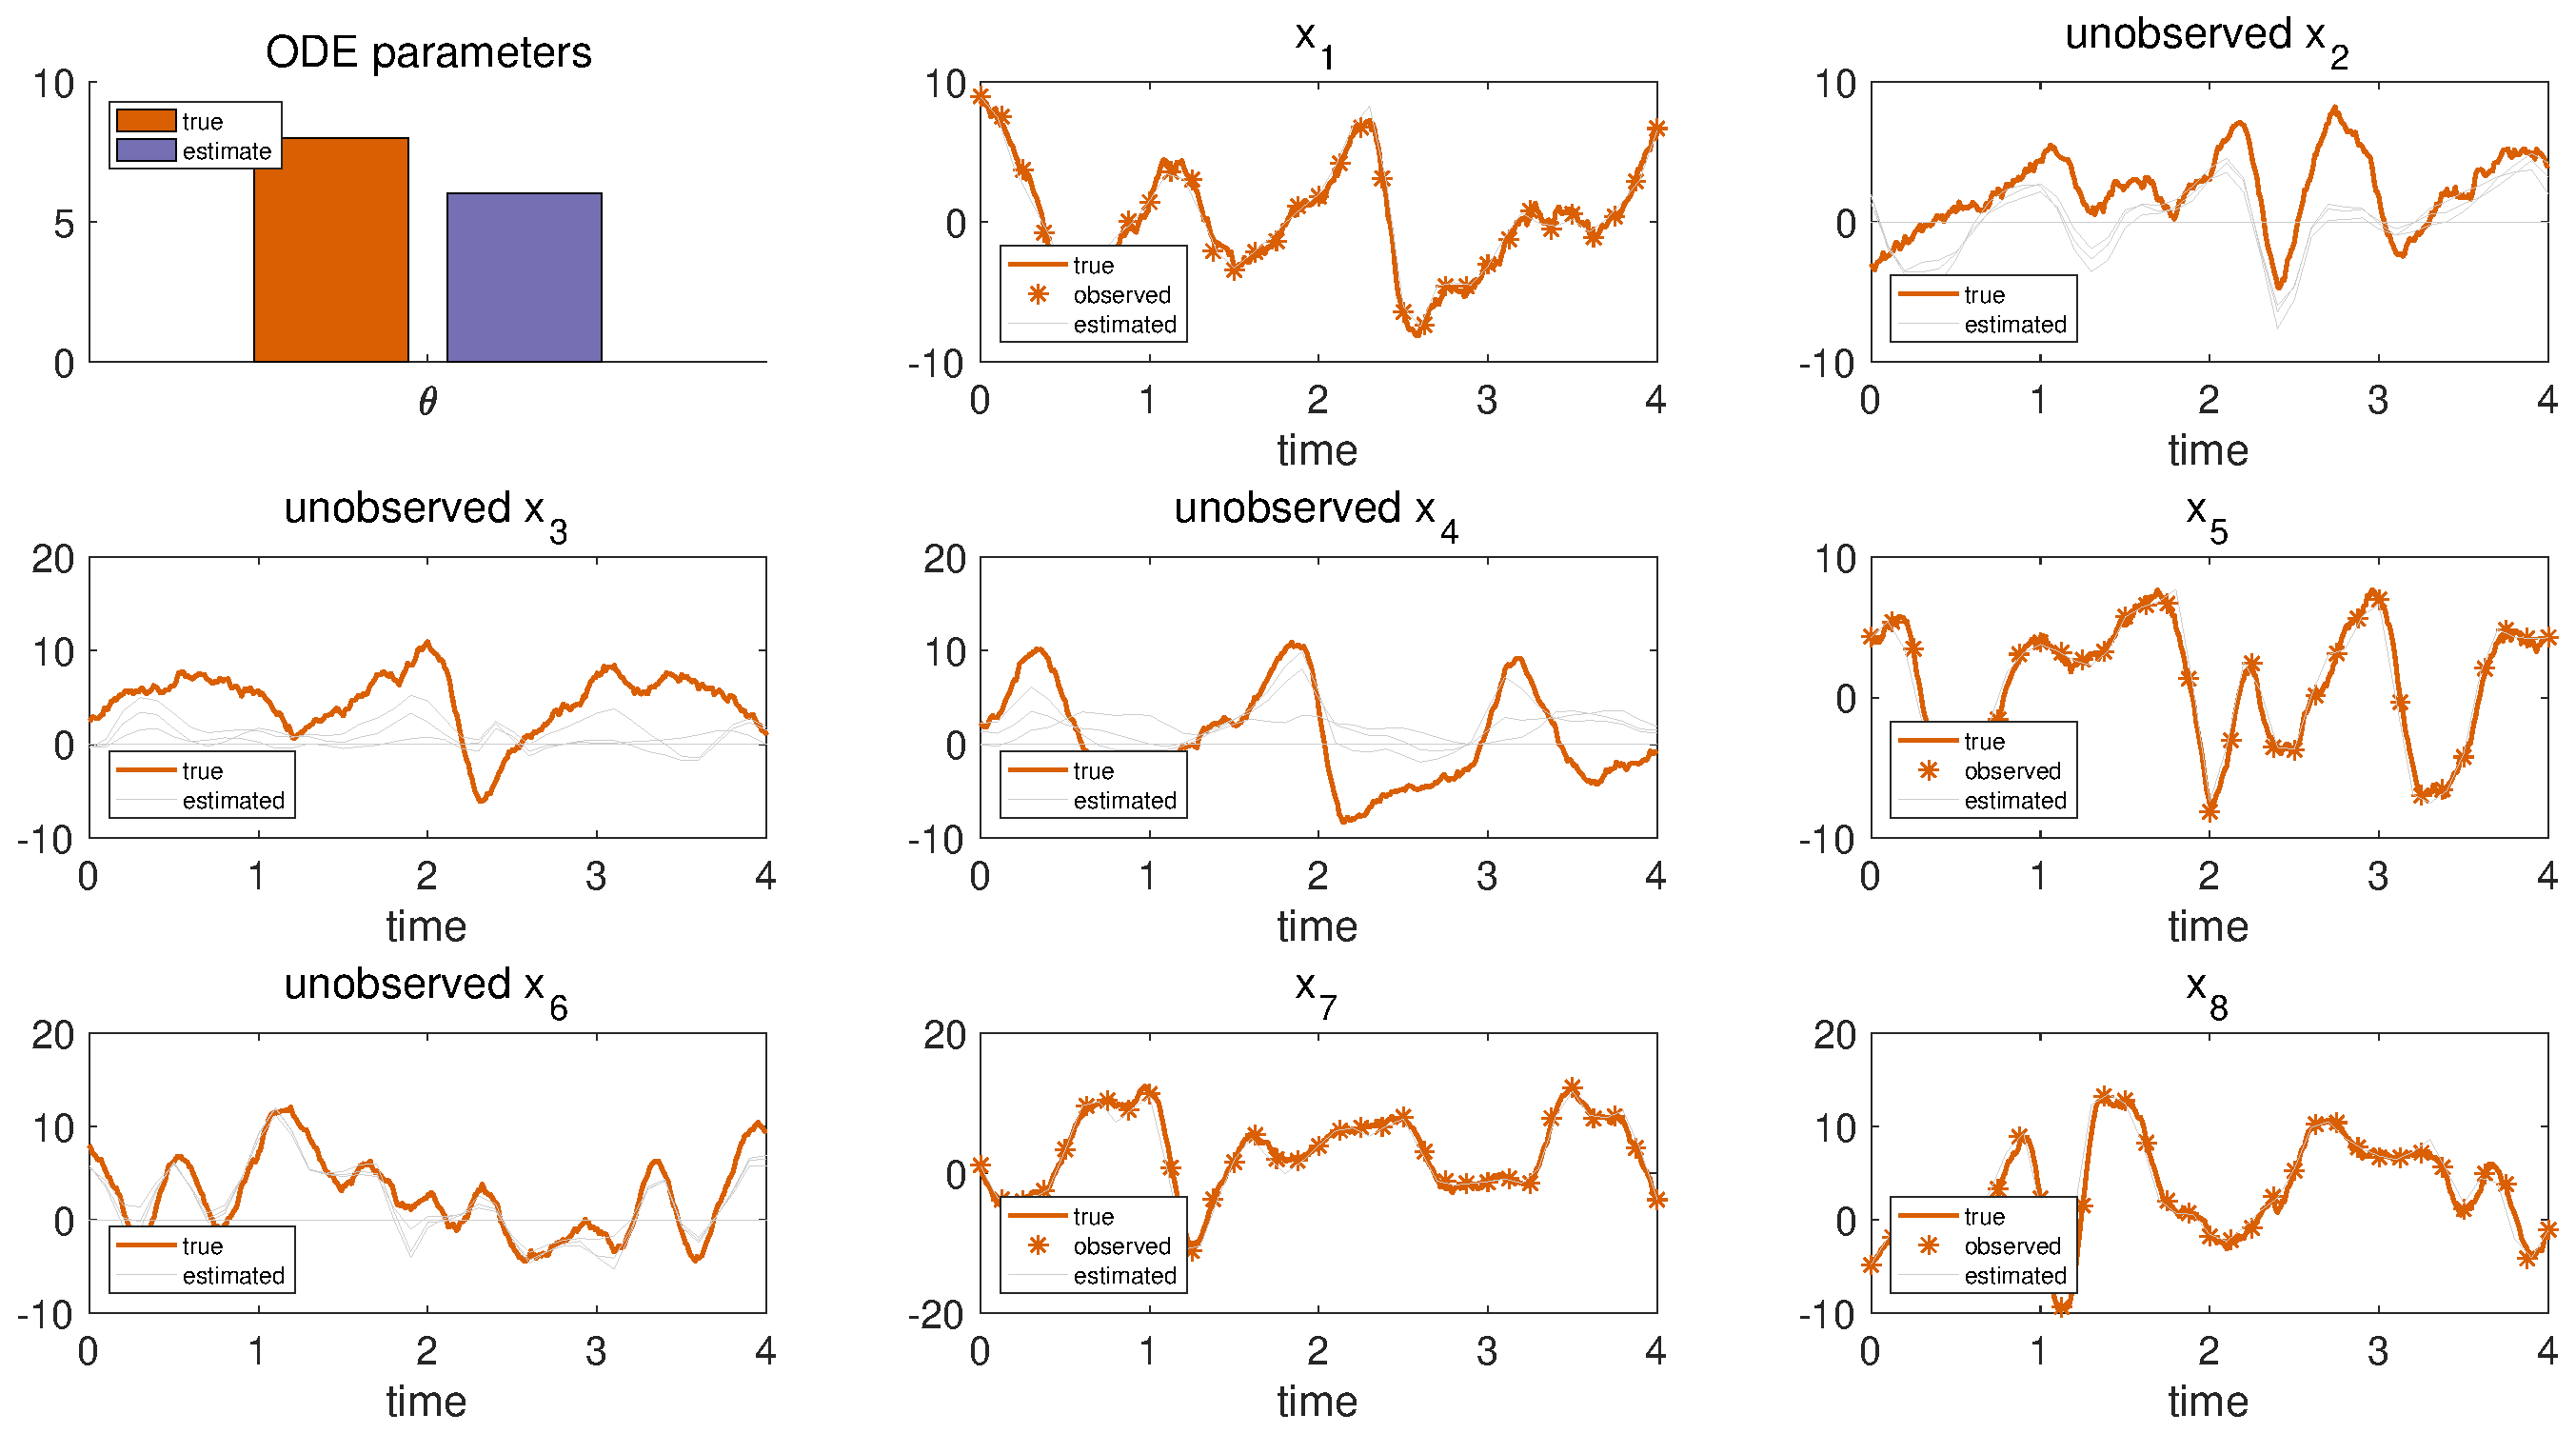
\includegraphics [width=5in]{Lorenz96_2_08.eps}

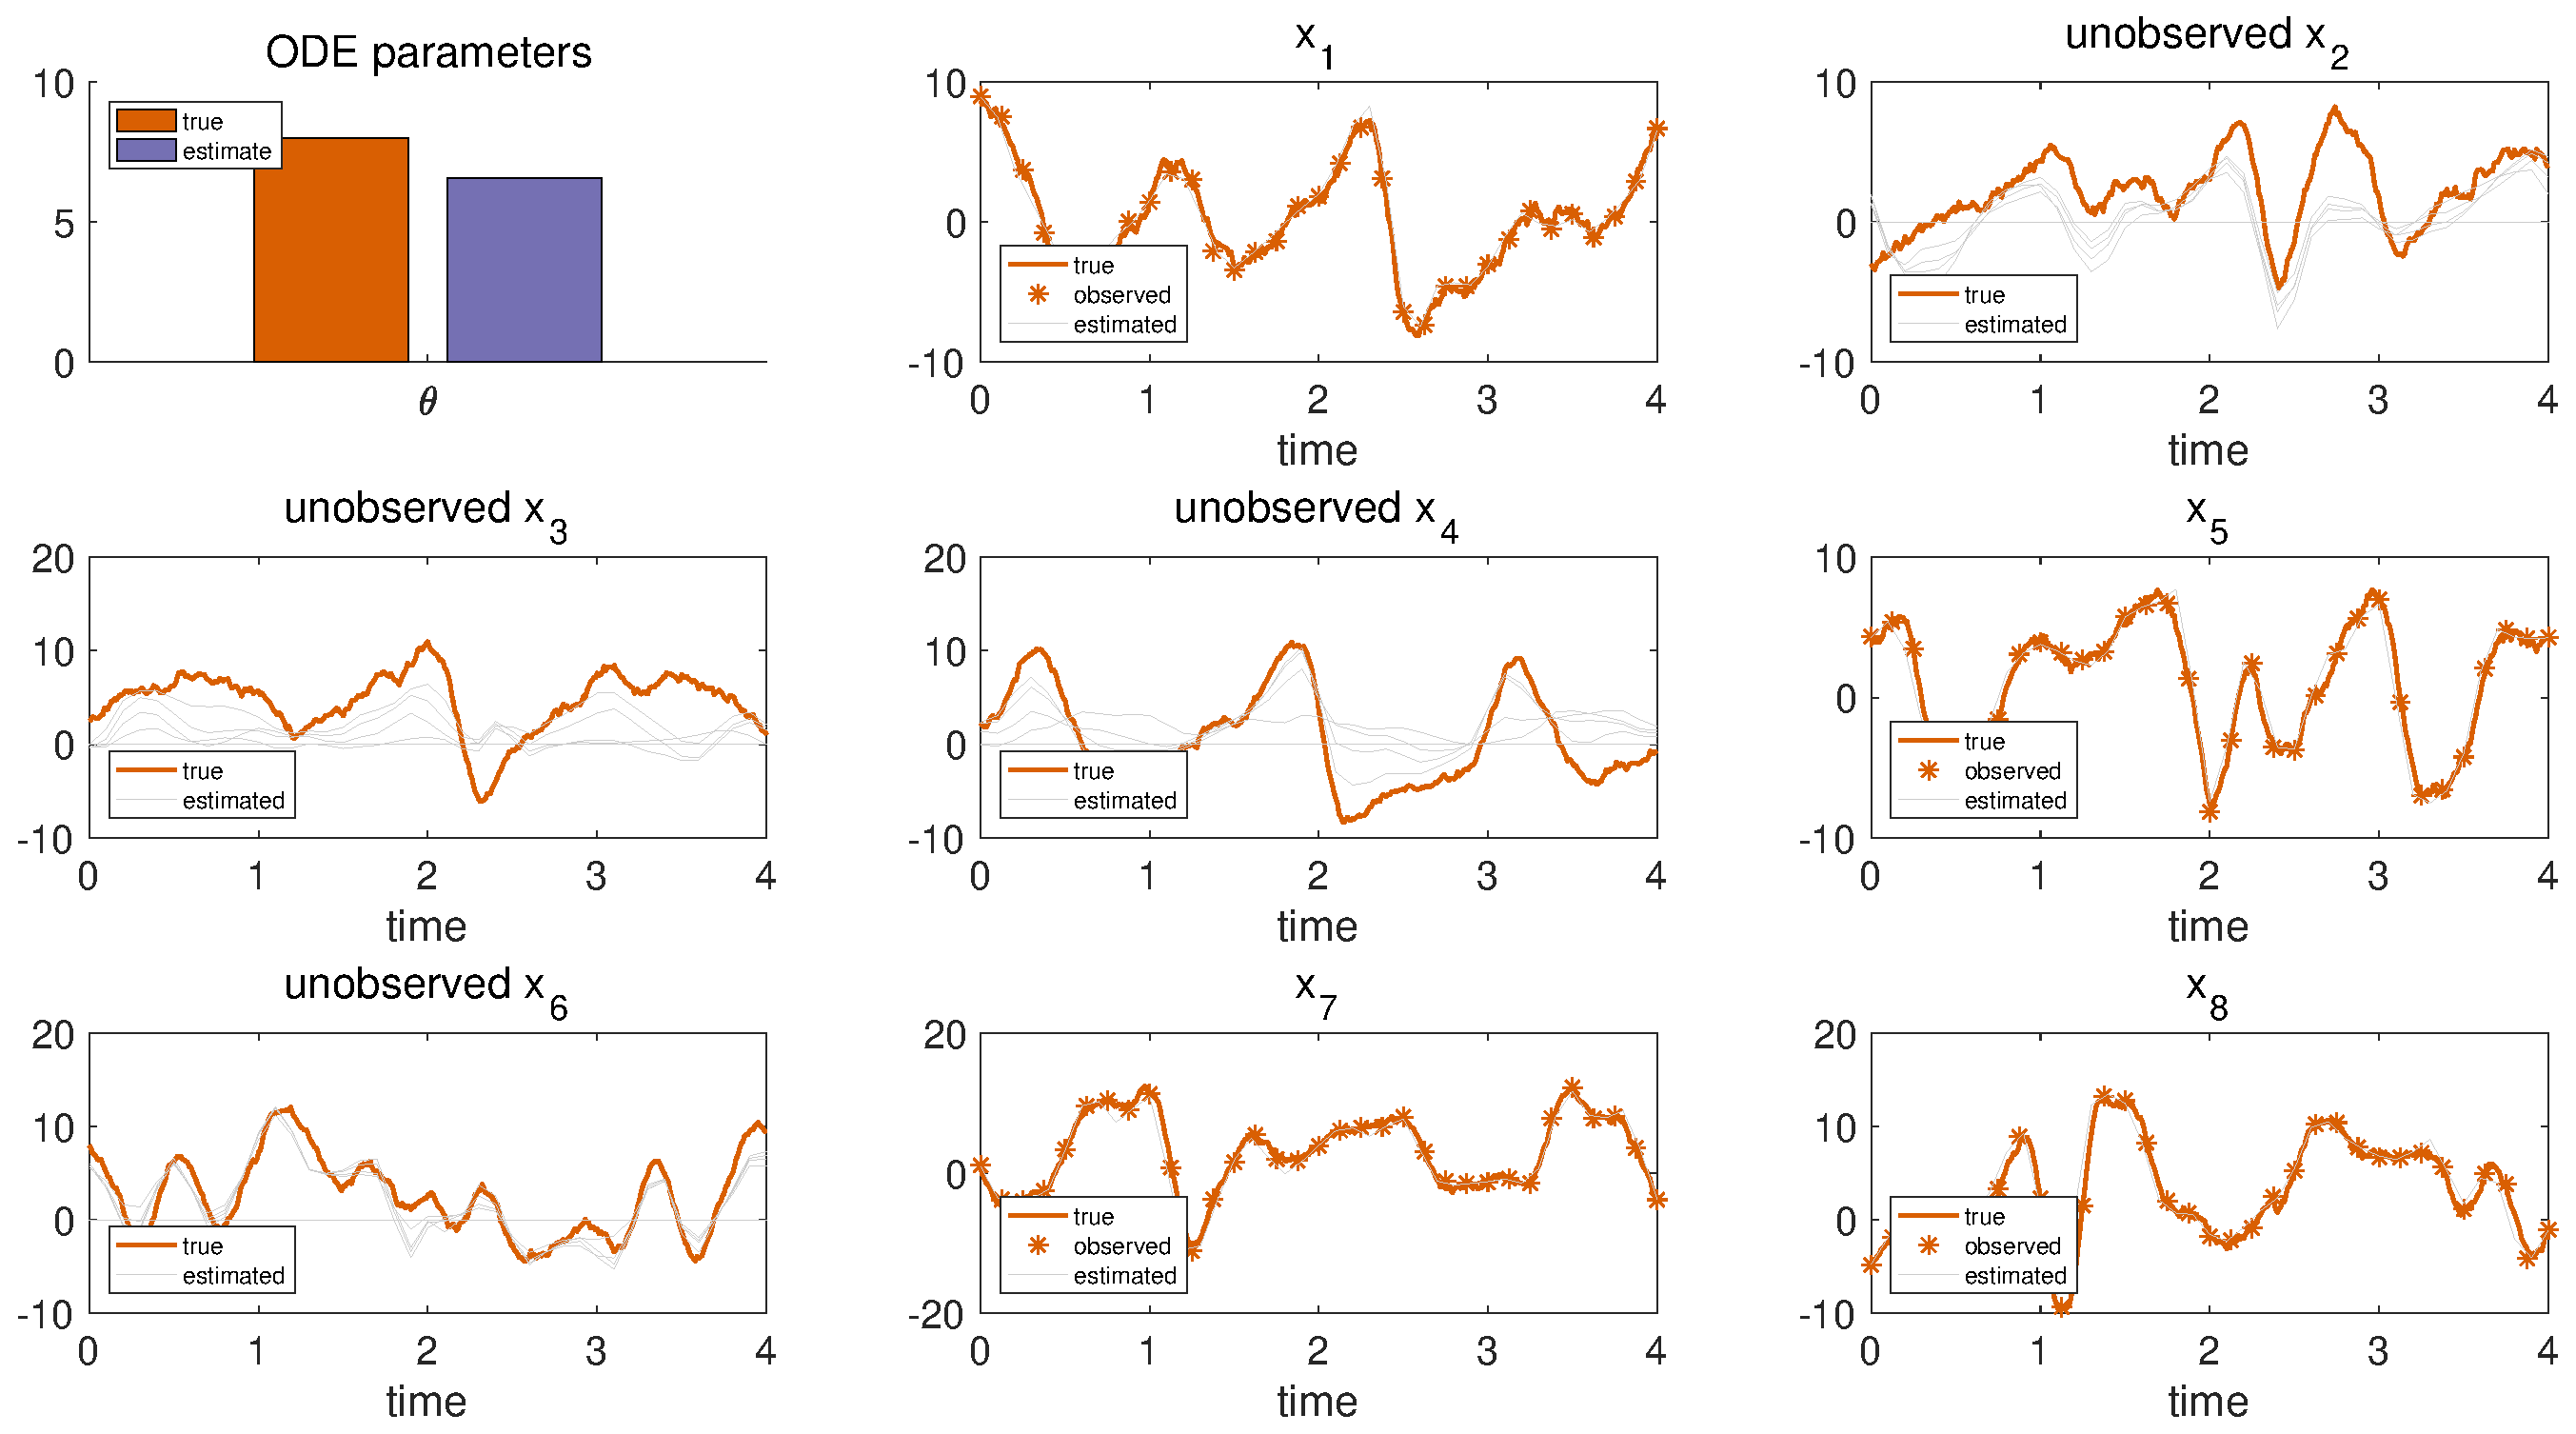
\includegraphics [width=5in]{Lorenz96_2_09.eps}

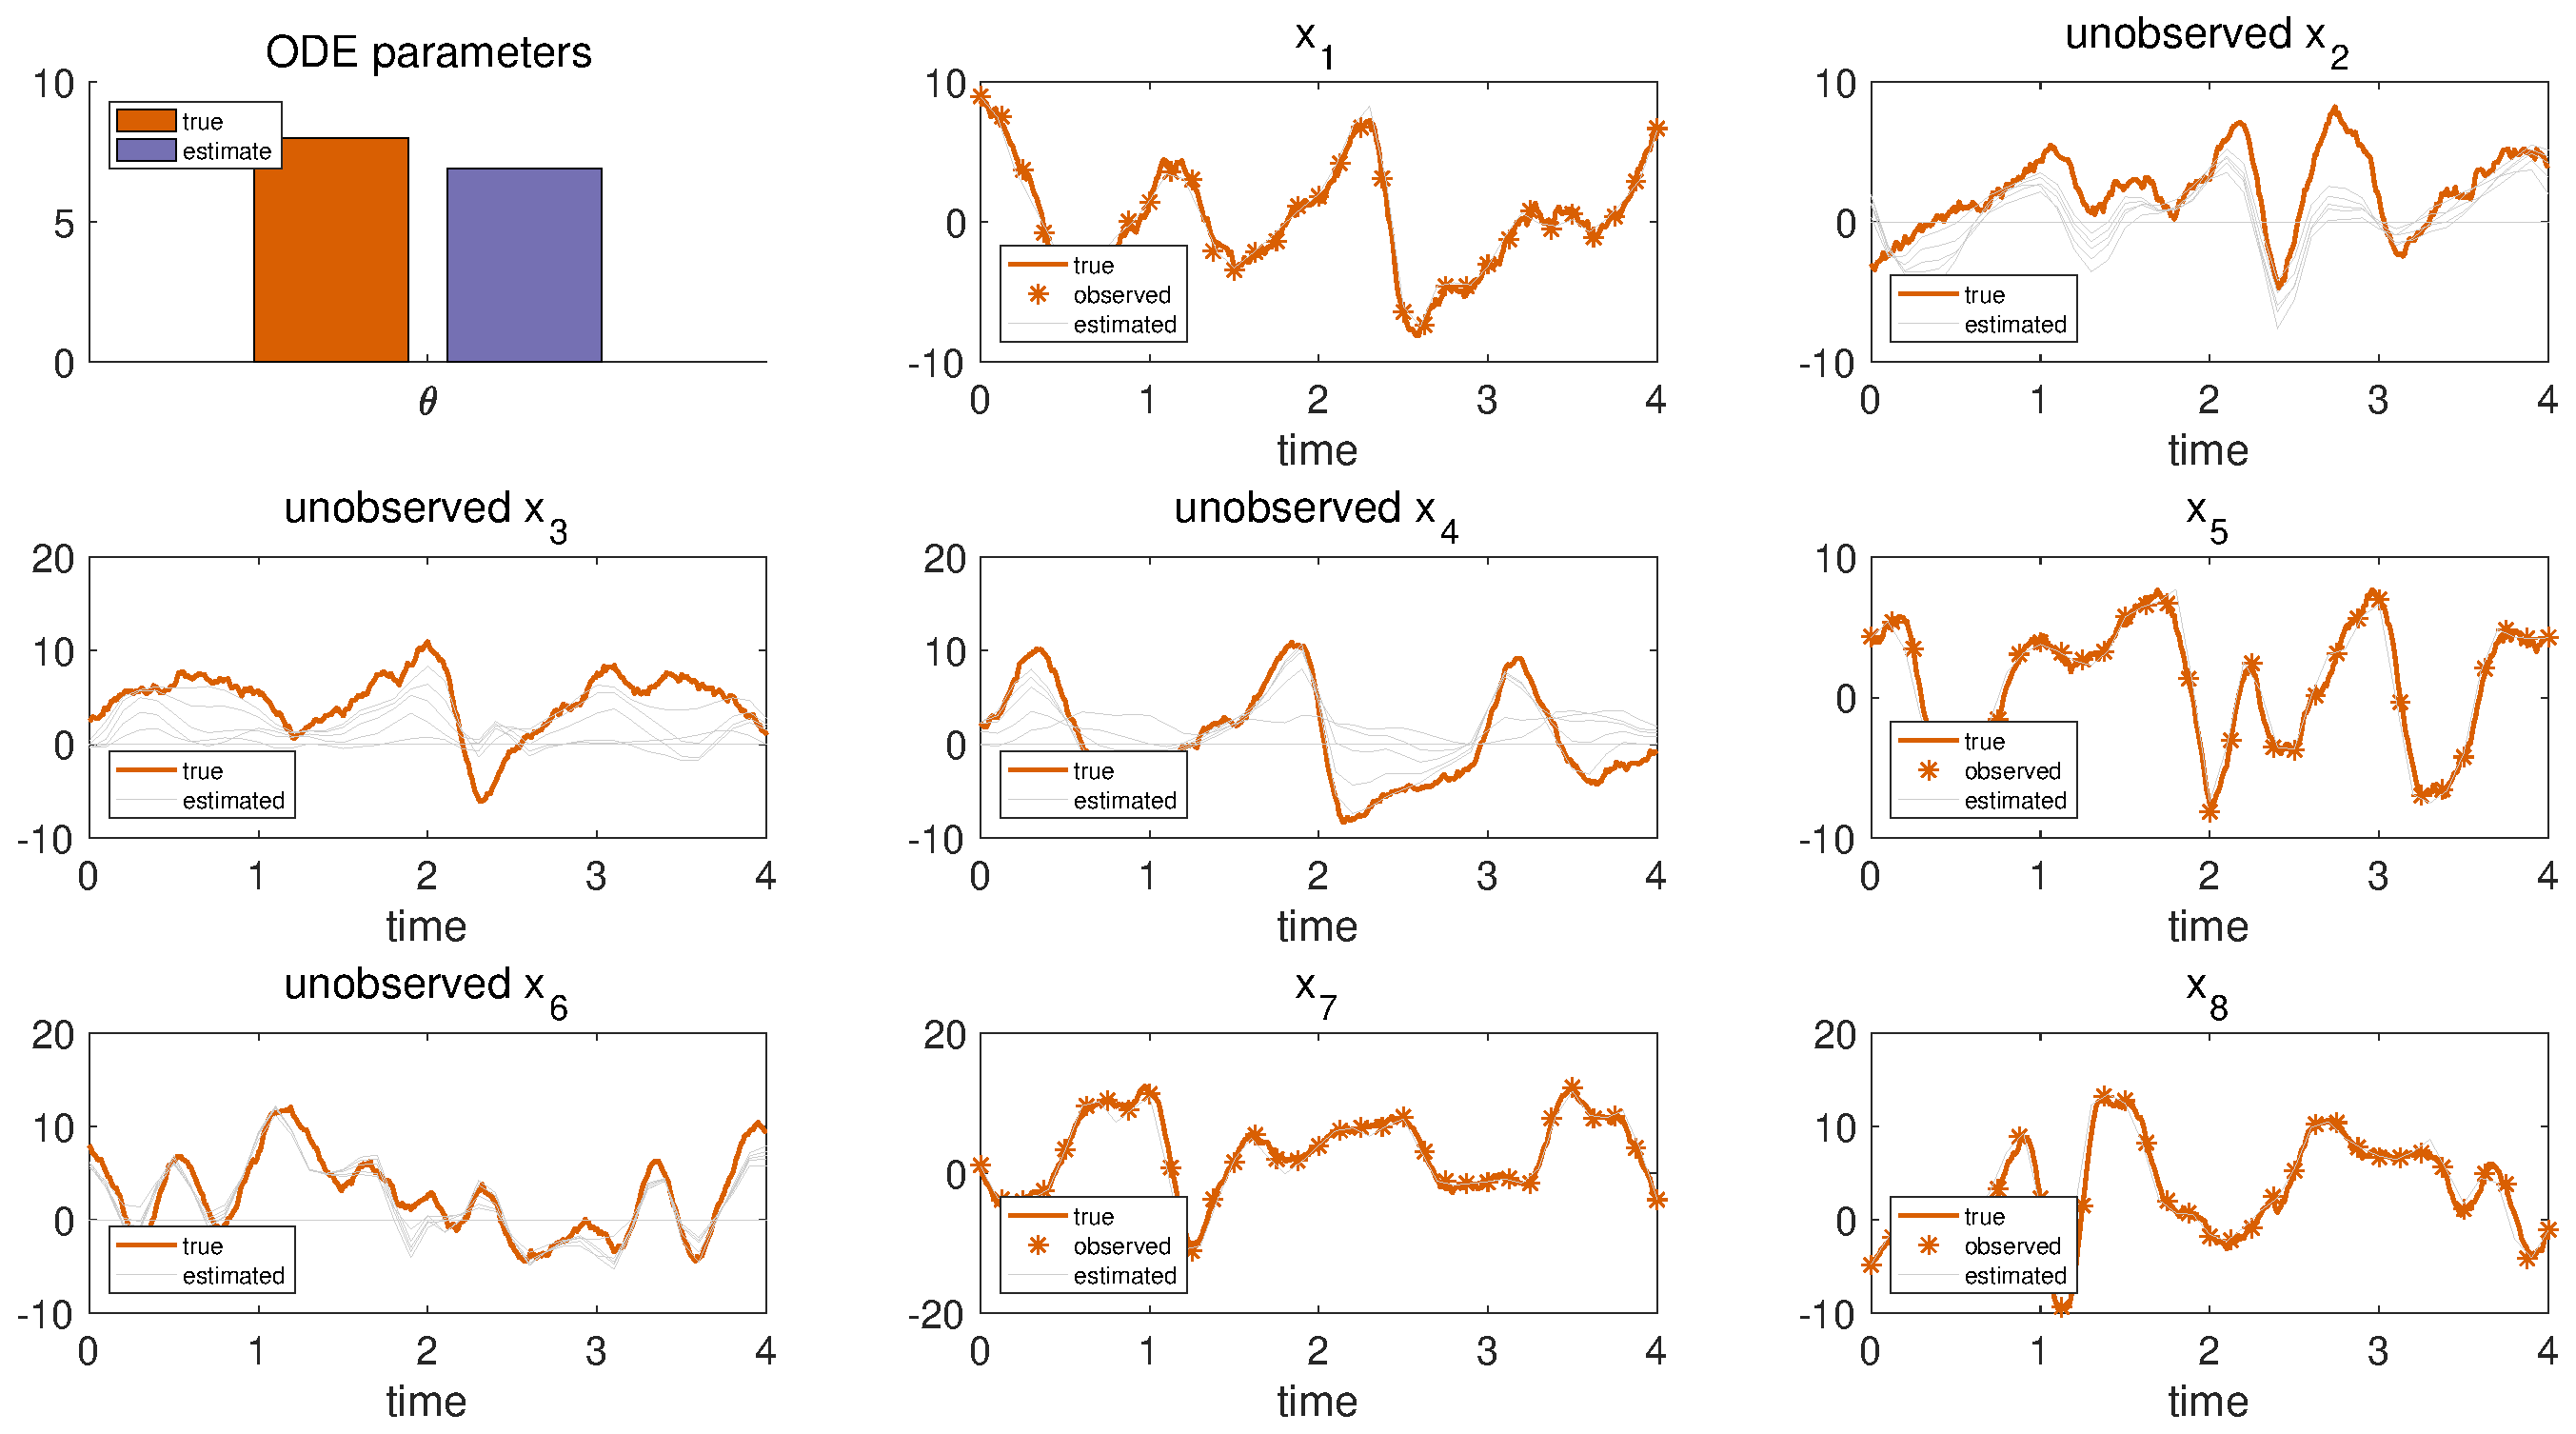
\includegraphics [width=5in]{Lorenz96_2_10.eps}

\includegraphics [width=5in]{Lorenz96_2_11.eps}

\includegraphics [width=5in]{Lorenz96_2_12.eps}

\includegraphics [width=5in]{Lorenz96_2_13.eps}

\includegraphics [width=5in]{Lorenz96_2_14.eps}
}

\color{black}
\color{RoyalPurple}\begin{verbatim}
end
\end{verbatim}
\color{black}
\begin{par}
\subsection{ Final result }
\end{par} \vspace{1em}
\color{RoyalPurple}\begin{verbatim}
plot_results(h_states,h_param,state,time,simulation,param_proxy_mean,p,symbols,'final');
\end{verbatim}
\color{black}

{
\centering
\includegraphics [width=5in]{Lorenz96_2_15.eps}
}

\section{Time Taken}

\color{RoyalPurple}\begin{verbatim}
disp(['time taken: ' num2str(toc) ' seconds'])
\end{verbatim}
\color{black}

        \begin{verbatim}time taken: 388.2428 seconds
\end{verbatim}
\color{black}
   
\cleardoublepage

  \setcounter{chapter}{3}
    \setcounter{section}{0}
\chapter*{VGM for Lorenz Attractor}
\phantomsection\addcontentsline{toc}{chapter}{VGM for Lorenz Attractor}
\section{Simulation Settings}

\color{RoyalPurple}\begin{verbatim}
simulation.state_obs_variance = @(mean)(bsxfun(@times,[2,2],...
    ones(size(mean))));              % observation noise
simulation.ode_param = [10,28,8/3];  % true ODE parameters;
simulation.final_time = 20;          % end time for integration
simulation.int_interval = 0.01;      % integration interval
simulation.time_samp = 0:0.1:simulation.final_time; % sample times for observations
simulation.init_val = -7.*ones(1,3); % initial state values

%symbols of observed states that appear in the 'ODEs.txt' file.
simulation.observed_states = {'[x]','[z]'};
\end{verbatim}
\color{black}


\section{User Input}

\begin{par}
\subsection{ Path to ODEs }
\end{par} \vspace{1em}
\color{RoyalPurple}\begin{verbatim}
odes_path = 'Lorenz_attractor_ODEs.txt';
\end{verbatim}
\color{black}
\begin{par}
\subsection{ Symbols } symbols of states and parameters in the '\_ODEs.txt' file
\end{par} \vspace{1em}
\begin{par}
States $\mathbf{x}$:
\end{par} \vspace{1em}
\color{RoyalPurple}\begin{verbatim}
symbols.state = {'[x]','[y]','[z]'}; % symbols of states in 'ODEs.txt' file
\end{verbatim}
\color{black}
\begin{par}
ODE parameters $\theta$ (symbols of parameters in 'ODEs.txt' file):
\end{par} \vspace{1em}
\color{RoyalPurple}\begin{verbatim}
symbols.param = {'[\sigma]','[\rho]','[\beta]'};
\end{verbatim}
\color{black}
\begin{par}
\subsection{ Kernel }
\end{par} \vspace{1em}
\begin{par}
Kernel parameters $\phi$:
\end{par} \vspace{1em}
\color{RoyalPurple}\begin{verbatim}
kernel.param = [10,0.2];             % set values of rbf kernel parameters
\end{verbatim}
\color{black}
\begin{par}
Error variance on state derivatives (i.e. $\gamma$):
\end{par} \vspace{1em}
\color{RoyalPurple}\begin{verbatim}
state.derivative_variance = 6*ones(1,length(symbols.state)); % gamma for gradient matching model
\end{verbatim}
\color{black}
\begin{par}
\subsection{ Estimation times }
\end{par} \vspace{1em}
\color{RoyalPurple}\begin{verbatim}
time.est = 0:0.1:20;                 % estimation times
\end{verbatim}
\color{black}
\begin{par}
\subsection{ Type of pseudo-inverse } Type of pseudo inverse; options: 'Moore-Penrose' or 'modified Moore-Penrose'
\end{par} \vspace{1em}
\color{RoyalPurple}\begin{verbatim}
opt_settings.pseudo_inv_type = 'Moore-Penrose';
\end{verbatim}
\color{black}
\begin{par}
\subsection{ Optimization settings }
\end{par} \vspace{1em}
\color{RoyalPurple}\begin{verbatim}
opt_settings.coord_ascent_numb_iter = 40;  % number of coordinate ascent iterations

% The observed state trajectories are clamped to the trajectories
% determined by standard GP regression (Boolean)
opt_settings.clamp_obs_state_to_GP_fit = true;
\end{verbatim}
\color{black}
\begin{par}
Plot settings: layout and size
\end{par} \vspace{1em}
\color{RoyalPurple}\begin{verbatim}
plot_settings.size = [1600, 800]; plot_settings.layout = [2,2];
\end{verbatim}
\color{black}


\section{Import ODEs}

\color{RoyalPurple}\begin{verbatim}
ode = import_odes(symbols,odes_path);
\end{verbatim}
\color{black}
\color{RoyalPurple}\begin{verbatim}
disp('ODEs:'); disp(ode.raw)
\end{verbatim}
\color{black}

        \begin{verbatim}ODEs:
    '[\sigma] .* ([y] - [x])'
    '[\rho] .* [x] - [y] - [x] .* [z]'
    '[x] .* [y] - [\beta] .* [z]'

\end{verbatim}
\color{black}


\section{Simulate Trajectory Observations}

\begin{par}
\subsection{ Generate ground truth by numerical integration }
\end{par} \vspace{1em}
\color{RoyalPurple}\begin{verbatim}
[state,time,ode] = generate_ground_truth(time,state,ode,symbols,simulation,...
    odes_path);
\end{verbatim}
\color{black}
\begin{par}
\subsection{ Generate state observations }
\end{par} \vspace{1em}
\color{RoyalPurple}\begin{verbatim}
if ~iscell(simulation.observed_states)
    ratio_observed = simulation.observed_states;
    state_obs_idx = zeros(1,simulation.numb_odes,'logical');
    idx = randperm(simulation.numb_odes);
    idx = idx(1:floor(simulation.numb_odes * ratio_observed));
    state_obs_idx(idx) = 1;
    simulation.observed_states = symbols.state(state_obs_idx);
end

[state,time,obs_to_state_relation] = generate_state_obs(state,time,simulation,...
    symbols);
\end{verbatim}
\color{black}
\begin{par}
\subsection{ Symbols }
\end{par} \vspace{1em}
\color{RoyalPurple}\begin{verbatim}
state.sym.mean = sym('x%d%d',[length(time.est),length(ode.system)]);
state.sym.variance = sym('sigma%d%d',[length(time.est),length(ode.system)]);
ode_param.sym.mean = sym('param%d',[length(symbols.param),1]);
assume(ode_param.sym.mean,'real');
\end{verbatim}
\color{black}
\begin{par}
\subsection{ Setup plots }
\end{par} \vspace{1em}
\begin{par}
Only the state dynamics are (partially) observed.
\end{par} \vspace{1em}
\color{RoyalPurple}\begin{verbatim}
[h_states,h_param,p] = setup_plots(state,time,simulation,symbols,plot_settings);

tic; %start timer
\end{verbatim}
\color{black}


\subsection{Prior on States and State Derivatives}

\color{RoyalPurple}\begin{verbatim}
[dC_times_invC,inv_C,A_plus_gamma_inv] = kernel_function(kernel,state,time.est);
\end{verbatim}
\color{black}


\section{State Couplings in ODEs}

\color{RoyalPurple}\begin{verbatim}
coupling_idx = find_state_couplings_in_odes(ode,symbols);
\end{verbatim}
\color{black}


\section{Rewrite ODEs as Linear Combination in Parameters}

\begin{par}
We rewrite the ODEs in equation (2) as a linear combination in the parameters:
\end{par} \vspace{1em}
\begin{par}
$\mathbf{B}_{\theta k} \theta + \mathbf{b}_{\theta k} \stackrel{!}{=} \mathbf{f}_k(\mathbf{X},\theta) \qquad (5)$,
\end{par} \vspace{1em}
\begin{par}
where matrices $\mathbf{B}_{\theta k}$ and $\mathbf{b}_{\theta k}$ are defined such that the ODEs $\mathbf{f}_k(\mathbf{X},\theta)$ are expressed as a linear combination in $\theta$.
\end{par} \vspace{1em}
\color{RoyalPurple}\begin{verbatim}
[ode_param.lin_comb.B,ode_param.lin_comb.b] = ...
    rewrite_odes_as_linear_combination_in_parameters(ode,symbols);
\end{verbatim}
\color{black}


\section{Rewrite ODEs as Linear Combination in Individual States}

\begin{par}
We rewrite the expression $\mathbf{f}(\mathbf{X},\theta) - {'\mathbf{C}}_{\phi} \mathbf{C}_{\phi}^{-1} \mathbf{X}$ in equation (4) as a linear combination in the individual state $\mathbf{x}_u$:
\end{par} \vspace{1em}
\begin{par}
$\mathbf{R}_{uk} \mathbf{x}_u + \mathbf{r}_{uk} \stackrel{!}{=} \mathbf{f}_k(\mathbf{X},\theta)$.
\end{par} \vspace{1em}
\begin{par}
where matrices $\mathbf{R}_{uk}$ and $\mathbf{r}_{uk}$ are defined such that the ODE $\mathbf{f}_k(\mathbf{X},\theta)$ is expressed as a linear combination in the individual state $\mathbf{x}_u$.
\end{par} \vspace{1em}
\color{RoyalPurple}\begin{verbatim}
[state.lin_comb.R,state.lin_comb.r] = ...
    rewrite_odes_as_linear_combination_in_ind_states(ode,symbols,coupling_idx.states);
\end{verbatim}
\color{black}



\section{Fitting observations of state trajectories}

\color{RoyalPurple}\begin{verbatim}
[mu,inv_sigma] = fitting_state_observations(state,inv_C,obs_to_state_relation,simulation);
\end{verbatim}
\color{black}


\section{Coordinate Ascent Variational Gradient Matching}

\begin{par}
We minimize the KL-divergence in equation (10) by coordinate descent (where each step is analytically tractable) by iterating between determining the proxy for the distribution over ODE parameters $\hat{q}(\theta)$ and the proxies for the distribution over individual states $\hat{q}(\mathbf{x}_u)$.
\end{par} \vspace{1em}
\color{RoyalPurple}\begin{verbatim}
state.proxy.mean = mu;  % Initialize the state estimation by the GP regression posterior
for i = 1:opt_settings.coord_ascent_numb_iter
\end{verbatim}
\color{black}

\subsection{ Proxy for ODE parameters }

\color{RoyalPurple}\begin{verbatim}
    [param_proxy_mean,param_proxy_inv_cov] = proxy_for_ode_parameters(state.proxy.mean,...
        dC_times_invC,ode_param.lin_comb,symbols,A_plus_gamma_inv,opt_settings);

    if i==1 || ~mod(i,1)
        plot_results(h_states,h_param,state,time,simulation,param_proxy_mean,...
            p,symbols,'not_final');
    end
\end{verbatim}
\color{black}

{
\centering
\includegraphics [width=5in]{Lorenz_attractor_4_05.eps}

\includegraphics [width=5in]{Lorenz_attractor_4_06.eps}

\includegraphics [width=5in]{Lorenz_attractor_4_07.eps}

\includegraphics [width=5in]{Lorenz_attractor_4_08.eps}

\includegraphics [width=5in]{Lorenz_attractor_4_09.eps}

\includegraphics [width=5in]{Lorenz_attractor_4_10.eps}

\includegraphics [width=5in]{Lorenz_attractor_4_11.eps}

\includegraphics [width=5in]{Lorenz_attractor_4_12.eps}

\includegraphics [width=5in]{Lorenz_attractor_4_13.eps}

\includegraphics [width=5in]{Lorenz_attractor_4_14.eps}

\includegraphics [width=5in]{Lorenz_attractor_4_15.eps}

\includegraphics [width=5in]{Lorenz_attractor_4_16.eps}

\includegraphics [width=5in]{Lorenz_attractor_4_17.eps}

\includegraphics [width=5in]{Lorenz_attractor_4_18.eps}

\includegraphics [width=5in]{Lorenz_attractor_4_19.eps}

\includegraphics [width=5in]{Lorenz_attractor_4_20.eps}

\includegraphics [width=5in]{Lorenz_attractor_4_21.eps}

\includegraphics [width=5in]{Lorenz_attractor_4_22.eps}

\includegraphics [width=5in]{Lorenz_attractor_4_23.eps}

\includegraphics [width=5in]{Lorenz_attractor_4_24.eps}

\includegraphics [width=5in]{Lorenz_attractor_4_25.eps}

\includegraphics [width=5in]{Lorenz_attractor_4_26.eps}

\includegraphics [width=5in]{Lorenz_attractor_4_27.eps}

\includegraphics [width=5in]{Lorenz_attractor_4_28.eps}

\includegraphics [width=5in]{Lorenz_attractor_4_29.eps}

\includegraphics [width=5in]{Lorenz_attractor_4_30.eps}

\includegraphics [width=5in]{Lorenz_attractor_4_31.eps}

\includegraphics [width=5in]{Lorenz_attractor_4_32.eps}

\includegraphics [width=5in]{Lorenz_attractor_4_33.eps}

\includegraphics [width=5in]{Lorenz_attractor_4_34.eps}

\includegraphics [width=5in]{Lorenz_attractor_4_35.eps}

\includegraphics [width=5in]{Lorenz_attractor_4_36.eps}

\includegraphics [width=5in]{Lorenz_attractor_4_37.eps}

\includegraphics [width=5in]{Lorenz_attractor_4_38.eps}

\includegraphics [width=5in]{Lorenz_attractor_4_39.eps}

\includegraphics [width=5in]{Lorenz_attractor_4_40.eps}

\includegraphics [width=5in]{Lorenz_attractor_4_41.eps}

\includegraphics [width=5in]{Lorenz_attractor_4_42.eps}

\includegraphics [width=5in]{Lorenz_attractor_4_43.eps}

\includegraphics [width=5in]{Lorenz_attractor_4_44.eps}
}

\subsection{ Proxy for individual states }

\color{RoyalPurple}\begin{verbatim}
    [state.proxy.mean,state.proxy.inv_cov] = proxy_for_ind_states(state.lin_comb,...
        state.proxy.mean,param_proxy_mean',dC_times_invC,coupling_idx.states,symbols,...
        mu,inv_sigma,simulation.observed_states,A_plus_gamma_inv,opt_settings);
\end{verbatim}
\color{black}
\color{RoyalPurple}\begin{verbatim}
end
\end{verbatim}
\color{black}
\begin{par}
\subsection{ Final result }
\end{par} \vspace{1em}
\color{RoyalPurple}\begin{verbatim}
plot_results(h_states,h_param,state,time,simulation,param_proxy_mean,p,symbols,'final');
\end{verbatim}
\color{black}

\begin{figure}[tbh!]
\centering
\includegraphics [width=5in]{Lorenz_attractor_4_45.eps}
\end{figure}

\section{Time Taken}

\color{RoyalPurple}\begin{verbatim}
disp(['time taken: ' num2str(toc) ' seconds'])
\end{verbatim}
\color{black}

        \begin{verbatim}time taken: 71.0552 seconds
\end{verbatim}
\color{black}
   
\cleardoublepage

  \setcounter{chapter}{4}
    \setcounter{section}{0}
\chapter*{VGM for Dynamic Causal Modeling}
\phantomsection\addcontentsline{toc}{chapter}{VGM for Dynamic Casual Modeling}
Example dynamical system used in this code: Dynamic Causal Modeling (\textbf{visual attention system}) with \textbf{three hidden neuronal- and 12 hidden hemodynamic states}. The system is affected by \textbf{given external inputs} and the states are only \textbf{indirectly observed} through the BOLD signal change equation.

\section{User Input}
\subsection{Simulation Settings}
\vspace{1em}
\begin{itemize}
   \item \textbf{Simulation ODEs}: Input the ODEs ``type'' used to generate the data as a string. Options: \begin{verbatim} 'nonlinear_forward_modulation_by_attention',
'forward_modulation_and_driven_by_attention', 
'forward_modulation_by_attention', 'backward_modulation_by_attention', 
'backward_modulation_and_driven_by_attention', 'absent_modulation', 
'absent_attention_input', 'absent_photic_input', 'driven_by_attention', 
'photic_input'.
\end{verbatim} 
    \color{RoyalPurple}\begin{verbatim}
simulation.odes = 'nonlinear_forward_modulation_by_attention';
\end{verbatim} 
\color{black}

   \item \textbf{Observed States}: Input a cell vector containing the symbols (characters) in the '*ODEs.txt' file. Eg: to observe deoxyhemoglobin content, blood volume and blood flow set \begin{verbatim} simulation.observed_states =   {'q_1','q_3','q_2','v_1','v_3','v_2',...
   'f_1','f_3','f_2'}).
\end{verbatim}
    \color{RoyalPurple}\begin{verbatim}
simulation.observed_states = {};
\end{verbatim} 
\color{black}

   \item \textbf{Final time for simulation}: Input a positive real number:
    \color{RoyalPurple}\begin{verbatim}
simulation.final_time = 359*3.22;
\end{verbatim} 
\color{black}

   \item \textbf{Observation noise}: Input a function handle:
    \color{RoyalPurple}\begin{verbatim}
simulation.state_obs_variance = @(x)(repmat(bsxfun(@rdivide,var(x),5),...
size(x,1),1));
\end{verbatim} 
\color{black}

   \item \textbf{Time interval between observations}: Input a positive real number:
    \color{RoyalPurple}\begin{verbatim}
simulation.interval_between_observations = 0.1;
\end{verbatim} 
\color{black}
\end{itemize}
\vspace{1em}


\subsection{Estimation Settings}
\vspace{1em}
\begin{itemize}
   \item \textbf{Candidate ODEs}: Input the ODEs ``type'' used to generate the data as a string. Options: \begin{verbatim} 'nonlinear_forward_modulation_by_attention', 
'forward_modulation_and_driven_by_attention', 
'forward_modulation_by_attention', 'backward_modulation_by_attention', 
'backward_modulation_and_driven_by_attention', 'absent_modulation', 
'absent_attention_input', 'absent_photic_input', 'driven_by_attention', 
'photic_input'.
\end{verbatim} 

\color{RoyalPurple}\begin{verbatim}
        candidate_odes = 'nonlinear_forward_modulation_by_attention';
\end{verbatim} 
\color{black}

   \item \textbf{Kernel parameters} $\boldsymbol\phi$: Input a row vector of positive real numbers of size 1 x 2:
    \color{RoyalPurple}\begin{verbatim}
kernel.param = [10,0.2];
\end{verbatim} 
\color{black}

   \item \textbf{Error variance on state derivatives (i.e. $\gamma$)}: Input a row vector of positive real numbers of size 1 x number of ODEs:
    \color{RoyalPurple}\begin{verbatim}
state.derivative_variance = 6.*ones(11-3,1);
\end{verbatim} 
\color{black}

\setlength{\itemsep}{-1ex}
   \item \textbf{Estimation times}: Input a row vector of positive real numbers in ascending order:
    \color{RoyalPurple}\begin{verbatim}
time.est = 0:3.22:359*3.22;
\end{verbatim} 
\color{black}
\end{itemize}
\vspace{2em}

\begin{par}
Preliminary operations
\end{par} \vspace{1em}
\color{RoyalPurple}\begin{verbatim}
close all; clc; addpath('VGM_functions')
\end{verbatim} 
\color{black}


\section{Preprocessing for candidate ODEs}

\color{RoyalPurple}\begin{verbatim}
[symbols,ode,plot_settings,state,simulation,odes_path,coupling_idx,opt_settings] = ...
    preprocessing_dynamic_causal_modeling (simulation,candidate_odes,state);
\end{verbatim} 
\color{black}
{\centering\small
        \color{MidnightBlue} \begin{verbatim} 
True ODEs:
 
/                                          / / 3 \exp(-f_1)     \   \
|                    25 exp(-q_1) exp(f_1) | | - |          - 1 |   |
|    d q_1                                 \ \ 5 /              /   |
|    ----- == - #3 - --------------------------------------------   |
|      dt                                 16                        |
|                                                                   |
|                                          / / 3 \exp(-f_3)     \   |
|                    25 exp(-q_3) exp(f_3) | | - |          - 1 |   |
|    d q_3                                 \ \ 5 /              /   |
|    ----- == - #1 - --------------------------------------------   |
|      dt                                 16                        |
|                                                                   |
|                                          / / 3 \exp(-f_2)     \   |
|                    25 exp(-q_2) exp(f_2) | | - |          - 1 |   |
|    d q_2                                 \ \ 5 /              /   |
|    ----- == - #2 - --------------------------------------------   |
|      dt                                 16                        |
|                                                                   |
|                 d v_1    5 exp(-v_1) exp(f_1)                     |
|                 ----- == -------------------- - #3                |
|                   dt               8                              |
|                                                                   |
|                 d v_3    5 exp(-v_3) exp(f_3)                     |
|                 ----- == -------------------- - #1                |
|                   dt               8                              |
|                                                                   |
|                 d v_2    5 exp(-v_2) exp(f_2)                     |
|                 ----- == -------------------- - #2                |
|                   dt               8                              |
|                                                                   |
|                       d f_1                                       |
|                       ----- == s_1 exp(-f_1)                      |
|                         dt                                        |
|                                                                   |
|                       d f_3                                       |
|                       ----- == s_3 exp(-f_3)                      |
|                         dt                                        |
|                                                                   |
|                       d f_2                                       |
|                       ----- == s_2 exp(-f_2)                      |
|                         dt                                        |
|                                                                   |
|               d s_1          3 s_1   8 exp(f_1)    8              |
|               ----- == n_1 - ----- - ---------- + --              |
|                 dt             5         25       25              |
|                                                                   |
|               d s_3          3 s_3   8 exp(f_3)    8              |
|               ----- == n_3 - ----- - ---------- + --              |
|                 dt             5         25       25              |
|                                                                   |
|               d s_2          3 s_2   8 exp(f_2)    8              |
|               ----- == n_2 - ----- - ---------- + --              |
|                 dt             5         25       25              |
|                                                                   |
|              d n_1                                                |
|              ----- == a_11 n_1 + a_12 n_2 + c_11 u_1              |
|                dt                                                 |
|                                                                   |
|              d n_3                                                |
|              ----- == a_32 n_2 + a_33 n_3 + c_33 u_3              |
|                dt                                                 |
|                                                                   |
| d n_2                                                             |
| ----- == a_22 n_2 + a_23 n_3 + n_1 (a_21 + d_213 n_3 + b_212 u_2) |
\   dt                                                              /

where

            / 17 v_3 \
         exp| ------ | 5
            \    8   /
   #1 == ---------------
                8

            / 17 v_2 \
         exp| ------ | 5
            \    8   /
   #2 == ---------------
                8

            / 17 v_1 \
         exp| ------ | 5
            \    8   /
   #3 == ---------------
                8


\end{verbatim} 
\color{black} 

}
    

\section{Simulate Trajectories}
\vspace{1em}
\begin{itemize}
   \item \textbf{Preprocessing for true ODEs}

\color{RoyalPurple}\begin{verbatim}
    [symbols_true,ode_true] = ...
    preprocessing_dynamic_causal_modeling (simulation,simulation.odes,state);
\end{verbatim} 
\color{black}
{\small\centering
        \color{MidnightBlue} \begin{verbatim} 
Candidate ODEs:
 
/                                          / / 3 \exp(-f_1)     \   \
|                    25 exp(-q_1) exp(f_1) | | - |          - 1 |   |
|    d q_1                                 \ \ 5 /              /   |
|    ----- == - #3 - --------------------------------------------   |
|      dt                                 16                        |
|                                                                   |
|                                          / / 3 \exp(-f_3)     \   |
|                    25 exp(-q_3) exp(f_3) | | - |          - 1 |   |
|    d q_3                                 \ \ 5 /              /   |
|    ----- == - #1 - --------------------------------------------   |
|      dt                                 16                        |
|                                                                   |
|                                          / / 3 \exp(-f_2)     \   |
|                    25 exp(-q_2) exp(f_2) | | - |          - 1 |   |
|    d q_2                                 \ \ 5 /              /   |
|    ----- == - #2 - --------------------------------------------   |
|      dt                                 16                        |
|                                                                   |
|                 d v_1    5 exp(-v_1) exp(f_1)                     |
|                 ----- == -------------------- - #3                |
|                   dt               8                              |
|                                                                   |
|                 d v_3    5 exp(-v_3) exp(f_3)                     |
|                 ----- == -------------------- - #1                |
|                   dt               8                              |
|                                                                   |
|                 d v_2    5 exp(-v_2) exp(f_2)                     |
|                 ----- == -------------------- - #2                |
|                   dt               8                              |
|                                                                   |
|                       d f_1                                       |
|                       ----- == s_1 exp(-f_1)                      |
|                         dt                                        |
|                                                                   |
|                       d f_3                                       |
|                       ----- == s_3 exp(-f_3)                      |
|                         dt                                        |
|                                                                   |
|                       d f_2                                       |
|                       ----- == s_2 exp(-f_2)                      |
|                         dt                                        |
|                                                                   |
|               d s_1          3 s_1   8 exp(f_1)    8              |
|               ----- == n_1 - ----- - ---------- + --              |
|                 dt             5         25       25              |
|                                                                   |
|               d s_3          3 s_3   8 exp(f_3)    8              |
|               ----- == n_3 - ----- - ---------- + --              |
|                 dt             5         25       25              |
|                                                                   |
|               d s_2          3 s_2   8 exp(f_2)    8              |
|               ----- == n_2 - ----- - ---------- + --              |
|                 dt             5         25       25              |
|                                                                   |
|              d n_1                                                |
|              ----- == a_11 n_1 + a_12 n_2 + c_11 u_1              |
|                dt                                                 |
|                                                                   |
|              d n_3                                                |
|              ----- == a_32 n_2 + a_33 n_3 + c_33 u_3              |
|                dt                                                 |
|                                                                   |
| d n_2                                                             |
| ----- == a_22 n_2 + a_23 n_3 + n_1 (a_21 + d_213 n_3 + b_212 u_2) |
\   dt                                                              /

where

            / 17 v_3 \
         exp| ------ | 5
            \    8   /
   #1 == ---------------
                8

            / 17 v_2 \
         exp| ------ | 5
            \    8   /
   #2 == ---------------
                8

            / 17 v_1 \
         exp| ------ | 5
            \    8   /
   #3 == ---------------
                8


\end{verbatim} 
\color{black} 

}

\item \textbf{Sample ODE parameters that lead to non-diverging trajectories}:

\color{RoyalPurple}\begin{verbatim}
non_diverging_trajectories = false; i = 0;
while ~non_diverging_trajectories
\end{verbatim} 
\color{black}

   \item \textbf{Sample ODE parameters}: Non-selfinhibitory neuronal couplings are sampled uniformly in the interval $[-0.8,0.8]$:
    \color{RoyalPurple}\begin{verbatim}
    simulation.ode_param = -0.8 + (0.8-(-0.8)) * rand(1,length(symbols_true.param));
    % simulation.ode_param = [0.46,0.13,0.39,0.26,0.5,0.26,0.1,1.25,-1,-1,-1];       
    % published ODE parameters (slightly modified from Stephan et al., 2008)
\end{verbatim} 
\color{black}

\item \textbf{Self-inhibitory neuronal couplings set to -1}:
    \color{RoyalPurple}\begin{verbatim}
    simulation.ode_param(end-2:end) = -1;
\end{verbatim} 
\color{black}

   \item \textbf{Numerical integration}

\color{RoyalPurple}\begin{verbatim}
    try
        simulation_old = simulation;
        [simulation,obs_to_state_relation,fig_handle,plot_handle] = ...
        simulate_state_dynamics_dcm(simulation,symbols_true,ode_true,...
        time,plot_settings,state.ext_input,'plot');
        non_diverging_trajectories = 1;
    end
\end{verbatim} 
\color{black}
\end{itemize}

{\centering
\includegraphics [width=6in]{VGM_for_dynamic_causal_modeling_01.eps}

\includegraphics [width=6in]{VGM_for_dynamic_causal_modeling_02.eps}

}
\color{RoyalPurple}\begin{verbatim}
end
\end{verbatim} 
\color{black}


\section{Mass Action Dynamical Systems}

\begin{par}
A deterministic dynamical system is represented by a set of $K$ ordinary differential equations (ODEs) with model parameters $\boldsymbol\theta \in \mathbb{R}^d$ that describe the evolution of $K$ states $\mathbf{x}(t) = [x_1(t),\ldots, x_K(t)]^T$ such that:
\end{par} \vspace{1em}
\begin{par}
$\dot{\mathbf{x}}(t) = \frac{d \mathbf{x}(t)}{d t} = \mathbf{f}(\mathbf{x}(t),\boldsymbol\theta), \qquad (1)$
\end{par} \vspace{1em}
\begin{par}
A sequence of observations, $\mathbf{y}(t)$, is usually contaminated by measurement error which we assume to be normally distributed with zero mean and variance for each of the $K$ states, i.e. $\mathbf{E}\sim\mathcal{N}(\mathbf{E};\mathbf{0},\mathbf{D})$, with $\mathbf{D}_{ik}=\sigma_k ^2 \delta_{ik}$. For $N$ distinct time points the overall system may therefore be summarized as
\end{par} \vspace{1em}
\begin{par}
$\mathbf{Y} = \mathbf{X} + \mathbf{E},$
\end{par} \vspace{1em}
\begin{par}
where
\end{par} \vspace{1em}
\begin{par}
$\mathbf{X} = [\mathbf{x}(t_1),\ldots,\mathbf{x}(t_N)] =  [\mathbf{x}_1,\ldots,\mathbf{x}_K]^T,$
\end{par} \vspace{1em}
\begin{par}
$\mathbf{Y} = [\mathbf{y}(t_1),\ldots,\mathbf{y}(t_N)] =  [\mathbf{y}_1,\ldots,\mathbf{y}_K]^T,$
\end{par} \vspace{1em}
\begin{par}
and $\mathbf{x}_k = [x_k(t_1),\ldots,x_k(t_N)]^T$ is the $k$'th state sequence and $\mathbf{y}_k = [y_k(t_1),\ldots,y_k(t_N)]^T$ are the observations. Given the observations $\mathbf{Y}$ and the description of the dynamical system (1), the aim is to estimate both state variables $\mathbf{X}$ and parameters $\boldsymbol\theta$.
\end{par} \vspace{1em}
\begin{par}
We consider only dynamical systems that are \textit{locally linear} w.r.t ODE parameters $\boldsymbol\theta$ and individual states $\mathbf{x}$. Such ODEs include mass-action kinetics and are given by:
\end{par} \vspace{1em}
\begin{par}
$f_{k}(\mathbf{x}(t),\theta) = \sum_{i=1} \theta_{ki} \prod_{j \in\mathcal{M}_{ki}} x_j, \qquad (2)$
\end{par} \vspace{1em}
\begin{par}

\noindent with $\mathcal{M}_{k_i} \subseteq \{ 1, \dots, K\}$ describing the state variables in each factor of the equation (i.e. the functions are linear in parameters and contain arbitrary large products of monomials of the states). 


\begin{par}
start timer
\end{par} \vspace{1em}
\color{RoyalPurple}\begin{verbatim}
tic;
\end{verbatim} 
\color{black}


\section{Prior on States and State Derivatives}

\begin{par}
Gradient matching with Gaussian processes assumes a joint Gaussian process prior on states and their derivatives:
\end{par} \vspace{1em}
\begin{par}
$\left(\begin{array}{c} \mathbf{X} \\ \dot{\mathbf{X}} \end{array}\right) \sim \mathcal{N} \left(\begin{array}{c} \mathbf{X} \\ \dot{\mathbf{X}} \end{array}~;~\begin{array}{c} \mathbf{0} \\\mathbf{0} \end{array}~,~\begin{array}{cc} \mathbf{C}_{\boldsymbol\phi} & \mathbf{C}_{\boldsymbol\phi}' \\ '\mathbf{C}_{\boldsymbol\phi} & \mathbf{C}_{\boldsymbol\phi}'' \end{array} \right) \qquad (3),$
\end{par} \vspace{1em}
\begin{par}
with
\end{par} \vspace{1em}
\begin{par}
$\mathrm{cov}(x_k(t), x_k(t)) = C_{\boldsymbol\phi_k}(t,t'),$
\end{par} \vspace{1em}
\begin{par}
$\mathrm{cov}(\dot{x}_k(t), x_k(t)) = \frac{\partial C_{\boldsymbol{\phi}_k}(t,t')}{\partial t} =: C_{{\boldsymbol\phi}_k}'(t,t'),$
\end{par} \vspace{1em}
\begin{par}
$\mathrm{cov}(x_k(t), \dot{x}_k(t)) = \frac{\partial C_{\boldsymbol\phi_k}(t,t')}{\partial t'} =: {'C_{\boldsymbol\phi_k}(t,t')},$
\end{par} \vspace{1em}
\begin{par}
$\mathrm{cov}(\dot{x}_k(t), \dot{x}_k(t)) = \frac{\partialC_{\boldsymbol\phi_k}(t,t') }{\partial t \partial t'} =: C_{\boldsymbol\phi_k}''(t,t').$
\end{par} \vspace{1em}


\section{Matching Gradients}

\begin{par}
Given the joint distribution over states and their derivatives (3) as well as the ODEs (2), we therefore have two expressions for the state derivatives:
\end{par} \vspace{1em}
\begin{par}
$\dot{\mathbf{X}} = \mathbf{F} + \boldsymbol\epsilon_1, \boldsymbol\epsilon_1 \sim\mathcal{N}\left(\boldsymbol\epsilon_1;\mathbf{0}, \mathbf{I}\gamma \right),$
\end{par} \vspace{1em}
\begin{par}
$\dot{\mathbf{X}} = {'\mathbf{C}_{\boldsymbol\phi}} \mathbf{C}_{\boldsymbol\phi}^{-1}~\mathbf{X} + \boldsymbol\epsilon_2, \boldsymbol\epsilon_2 \sim\mathcal{N}\left(\boldsymbol\epsilon_2;\mathbf{0}, \mathbf{A} \right),$
\end{par} \vspace{1em}
\begin{par}
where $\mathbf{F} := \mathbf{f}(\mathbf{X},\boldsymbol\theta)$ and $\mathbf{A} :=\mathbf{C}_{\boldsymbol\phi}'' -  {'\mathbf{C}_{\boldsymbol\phi}} \mathbf{C}_{\boldsymbol\phi}^{-1}\mathbf{C}_{\boldsymbol\phi}'$ and $\gamma$ is the error variance in the ODEs. Note that, in a deterministic system, the output of the ODEs $\mathbf{F}$ should equal the state derivatives $\dot{\mathbf{X}}$. However, in the first equation above we relax this contraint by adding stochasticity to the state derivatives $\dot{\mathbf{X}}$ in order to compensate for a potential model mismatch. The second equation above is obtained by deriving the conditional distribution for $\dot{\mathbf{X}}$ from the joint distribution in equation (3). Equating the two expressions in the equations above we can eliminate the unknown state derivatives $\dot{\mathbf{X}$:
\end{par} \vspace{1em}
\begin{par}
$\mathbf{F} = {'\mathbf{C}_{\boldsymbol\phi}} \mathbf{C}_{\boldsymbol\phi}^{-1} ~\mathbf{X} +\boldsymbol\epsilon_0, \qquad (4)$
\end{par} \vspace{1em}
\begin{par}
with $\boldsymbol{\epsilon}_0 := \mathbf{\epsilon_2} - \mathbf{\epsilon_1}$.
\end{par} \vspace{1em}
\color{RoyalPurple}\begin{verbatim}
[dC_times_invC,inv_C,A_plus_gamma_inv] = kernel_function(kernel,state,time.est);
\end{verbatim} 
\color{black}


\section{Rewrite ODEs as Linear Combination in Parameters}

\begin{par}
Since, according to the mass action dynamics (equation 2), the ODEs are \textit{linear in the parameters} $\boldsymbol\theta$ we can rewrite the ODEs in equation (2) as a linear combination in the parameters:
\end{par} \vspace{1em}
\begin{par}
$\mathbf{B}_{\boldsymbol{\theta} k} \boldsymbol{\theta} + \mathbf{b}_{\boldsymbol{\theta} k} \stackrel{!}{=}\mathbf{f}_k(\mathbf{X},\boldsymbol{\theta}), \qquad (5)$
\end{par} \vspace{1em}
\begin{par}
where matrices $\mathbf{B}_{\boldsymbol{\theta} k}$ and $\mathbf{b}_{\boldsymbol{\theta} k}$ are defined such that the ODEs $\mathbf{f}_k(\mathbf{X},\boldsymbol{\theta})$ are expressed as a linear combination in $\boldsymbol{\theta}$.
\end{par} \vspace{1em}
\color{RoyalPurple}\begin{verbatim}
[ode_param.lin_comb.B,ode_param.lin_comb.b] = ...
rewrite_odes_as_linear_combination_in_parameters(ode,symbols);
\end{verbatim} 
\color{black}


\section{Posterior over ODE Parameters}

\begin{par}
Inserting (5) into (4) and solving for $\boldsymbol{\theta}$ yields:
\end{par} \vspace{1em}
\begin{par}
$\boldsymbol{\theta} = \mathbf{B}_{\boldsymbol{\theta}}^+ \left( {'\mathbf{C}_{\boldsymbol{\phi}}}\mathbf{C}_{\boldsymbol{\phi}}^{-1} \mathbf{X} - \mathbf{b}_{\boldsymbol{\theta}} + \boldsymbol{\epsilon}_0\right),$
\end{par} \vspace{1em}
\begin{par}
where $\mathbf{B}_{\boldsymbol{\theta}}^+$ denotes the pseudo-inverse of $\mathbf{B}_{\boldsymbol{\theta}}$. Since $\mathbf{C}_{\boldsymbol{\phi}}$ is block diagonal we can rewrite the expression above as:
\end{par} \vspace{1em}
\begin{par}
$\boldsymbol{\theta} = \left( \mathbf{B}_{\boldsymbol{\theta}}^T \mathbf{B}_{\boldsymbol{\theta}} \right)^{-1} ~\mathbf{B}_{\boldsymbol{\theta}}^T  \left( \sum_k {'\mathbf{C}_{\boldsymbol{\phi}_k}}\mathbf{C}_{\boldsymbol{\phi}_k}^{-1} \mathbf{X}_k - \mathbf{b}_{\boldsymbol{\theta} k} + \boldsymbol{\epsilon}_0^{(k)} \right)\\ ~= \left( \mathbf{B}_{\boldsymbol{\theta}}^T \mathbf{B}_{\boldsymbol{\theta}} \right)^{-1} \left(\sum_k \mathbf{B}_{\boldsymbol{\theta} k}^T \left( {'\mathbf{C}_{\boldsymbol{\phi}_k}}\mathbf{C}_{\boldsymbol{\phi}_k}^{-1} \mathbf{X}_k - \mathbf{b}_{\boldsymbol{\theta} k} +\boldsymbol{\epsilon}_0^{(k)} \right) \right),$
\end{par} \vspace{1em}
\begin{par}
where we subsitute the Moore-Penrose inverse for the pseudo-inverse (i.e. $\mathbf{B}_{\boldsymbol{\theta}}^+ := \left( \mathbf{B}_{\boldsymbol{\theta}}^T \mathbf{B}_{\boldsymbol{\theta}}\right)^{-1} \mathbf{B}_{\boldsymbol{\theta}}^T$). We can therefore derive the posterior distribution over ODE parameters:
\end{par} \vspace{1em}
\begin{par}
$p(\boldsymbol{\theta} \mid \mathbf{X}, \boldsymbol{\phi}, \gamma) = \mathcal{N}\left(\boldsymbol{\theta} ; \left( \mathbf{B}_{\boldsymbol{\theta}}^T\mathbf{B}_{\boldsymbol{\theta}} \right)^{-1} \left( \sum_k \mathbf{B}_{\boldsymbol{\theta} k}^T ~\left( {'\mathbf{C}_{\boldsymbol{\phi} k}} \mathbf{C}_{\boldsymbol{\phi} k}^{-1} \mathbf{X}_k -\mathbf{b}_{\boldsymbol{\theta} k} \right) \right), ~ \mathbf{B}_{\boldsymbol{\theta}}^+ ~(\mathbf{A} + \mathbf{I}\gamma) ~ \mathbf{B}_{\boldsymbol{\theta}}^{+T} \qquad (6).$
\end{par} 


\section{Rewrite Hemodynamic ODEs as Linear Combination in (monotonic functions of) Individual Hemodynamic States}

\subsection{Rewrite the BOLD Signal Change Equation as a Linear Combination in a Monotonic Function of the Deoxyhemoglobin Content $\exp(\mathbf{q})$}

$$\mathbf{R}_{q~\mathbf\lambda} ~ \exp(\mathbf{q}) ~+ ~
\mathbf{r}_{v~\mathbf\lambda} \stackrel{!}{=} ~\mathbf\lambda(\mathbf{q},\mathbf{v}).$$
    \color{RoyalPurple}\begin{verbatim}
[state.deoxyhemo.R,state.deoxyhemo.r] = ...
rewrite_bold_signal_eqn_as_linear_combination_in_deoxyhemo(symbols);
\end{verbatim} 
\color{black}

\subsection{Rewrite the Deoxyhemoglobin Content ODE as a Linear Combination in a Monotonic Function of the Blood Volume $\exp\left( 17 / 8 ~\mathbf{v}\right)$}

$$\mathbf{R}_{v\dot{q}} ~\exp\left( 17 / 8 ~\mathbf{v}\right)
~+~ \mathbf{r}_{v\dot{q}} \stackrel{!}{=} \mathbf{f}_{\dot{q}}(\mathbf{X},\boldsymbol\theta).$$
    \color{RoyalPurple}\begin{verbatim}
[state.vol.R,state.vol.r] = rewrite_deoxyhemo_ODE_as_linear_combination_in_vol(...
ode,symbols);
\end{verbatim} 
\color{black}

\subsection{Rewrite the Blood Volume ODE as a Linear Combination in a Monotonic Function of the Blood Flow $\exp(\mathbf{f})$}
    
$$\mathbf{R}_{f~\dot{v}} ~ \exp(\mathbf{f}) + \mathbf{r}_{f~\dot{v}}
\stackrel{!}{=} \mathbf{f}_{\dot{v}}(\mathbf{X},\boldsymbol\theta).$$
    \color{RoyalPurple}\begin{verbatim}
[state.flow.R,state.flow.r] = rewrite_vol_ODE_as_linear_combination_in_flow(...
ode,symbols);
\end{verbatim} 
\color{black}
\subsection{Rewrite the Blood Flow and Vasosignalling ODEs as a linear combination in Vasosignalling $\mathbf{s}$}
    
$$\mathbf{R}_{s\dot{f}} ~\mathbf{s} + \mathbf{r}_{s\dot{f}}
\stackrel{!}{=} \mathbf{f}_{\dot{f}}(\mathbf{X},\boldsymbol\theta), \qquad \mathbf{R}_{s\dot{s}}~ \mathbf{s} + \mathbf{r}_{ \dot{s}} \stackrel{!}{=} \mathbf{f}_{\dot{s}}(\mathbf{X},\boldsymbol\theta).$$
    \color{RoyalPurple}\begin{verbatim}
[state.vaso.R,state.vaso.r] = ...
rewrite_vaso_and_flow_odes_as_linear_combination_in_vaso(ode,symbols);
\end{verbatim} 
\color{black}


\section{Rewrite Neuronal ODEs as Linear Combination in Individual Neuronal States}

\begin{par}
We rewrite the ODE(s) $\mathbf{f}_k(\mathbf{X},\boldsymbol\theta)$ as a linear combination in the individual state $\mathbf{n}_u$:
\end{par} \vspace{1em}

$$\mathbf{R}_{uk}  \mathbf{n}_u + \mathbf{r}_{uk} \stackrel{!}{=}
\mathbf{f}_{k}(\mathbf{X},\boldsymbol\theta),$$
    \begin{par}
where matrices $\mathbf{R}_{uk}$ and $\mathbf{r}_{uk}$ are defined such that the ODE $\mathbf{f}_k(\mathbf{X},\boldsymbol\theta)$ is expressed as a linear combination in the individual state $\mathbf{n}_u$.
\end{par} \vspace{1em}

\color{RoyalPurple}\begin{verbatim}
[state.neuronal.R,state.neuronal.r] = ...
rewrite_odes_as_linear_combination_in_ind_neuronal_states(ode,symbols,...
coupling_idx.states);
\end{verbatim} 
\end{par}


\section{Posterior over Individual States}

\begin{par}
Given the linear combination of the ODEs w.r.t. an individual state, we define the matrices $\mathbf{B}_u$ and $\mathbf{b}_u$ such that the expression $\mathbf{f}(\mathbf{X},\boldsymbol{\theta}) - {'\mathbf{C}}_{\boldsymbol{\phi}}\mathbf{C}_{\boldsymbol{\phi}}^{-1} \mathbf{X}$ is rewritten as a linear combination in an individual state $\mathbf{x}_u$:
\end{par} \vspace{1em}
\begin{par}
$\mathbf{B}_{u} \mathbf{x}_u + \mathbf{b}_{u} \stackrel{!}{=}\mathbf{f}(\mathbf{X},\boldsymbol{\theta}) - {'\mathbf{C}}_{\boldsymbol{\phi}}\mathbf{C}_{\boldsymbol{\phi}}^{-1} \mathbf{X} \qquad (7)$.
\end{par} \vspace{1em}
\begin{par}
Inserting (7) into (4) and solving for $\mathbf{x}_u$ yields:
\end{par} \vspace{1em}
\begin{par}
$\mathbf{x}_u = \mathbf{B}_{u}^+ \left( \boldsymbol{\epsilon}_0 -\mathbf{b}_{u}\right)$,
\end{par} \vspace{1em}
\begin{par}
where $\mathbf{B}_{u}^+$ denotes the pseudo-inverse of $\mathbf{B}_{u}$. Since $\mathbf{C}_{\boldsymbol{\phi}}$ is block diagonal we can rewrite the expression above as:
\end{par} \vspace{1em}
\begin{par}
$\mathbf{x}_u = \left( \mathbf{B}_{u} \mathbf{B}_{u}^T \right)^{-1}\mathbf{B}_{u}^T \sum_k \left(\boldsymbol{\epsilon}_0^{(k)} -\mathbf{b}_{uk} \right)\\ \quad= \left( \mathbf{B}_{u} \mathbf{B}_{u}^T \right)^{-1} \sum_k\mathbf{B}_{uk}^T \left(\boldsymbol{\epsilon}_0^{(k)} -\mathbf{b}_{uk} \right)$,
\end{par} \vspace{1em}
\begin{par}
where we substitute the Moore-Penrose inverse for the pseudo-inverse (i.e. $\mathbf{B}_{\boldsymbol{\theta}}^+ := \left( \mathbf{B}_{\boldsymbol{\theta}}^T \mathbf{B}_{\boldsymbol{\theta}}\right)^{-1} \mathbf{B}_{\boldsymbol{\theta}}^T$).  We can therefore derive the posterior distribution over an individual state $\mathbf{x}_{u}$:
\end{par} \vspace{1em}
\begin{par}
$p(\mathbf{x}_u \mid \mathbf{X}_{-u}, \boldsymbol{\phi}, \gamma)= \mathcal{N}\left(\mathbf{x}_u ; \left( \mathbf{B}_{u} \mathbf{B}_{u}^T\right)^{-1} \left( - \sum_k \mathbf{B}_{uk}^T \mathbf{b}_{uk} \right),~\mathbf{B}_{u}^{+} ~ (\mathbf{A} + \mathbf{I}\gamma) ~ \mathbf{B}_u^{+T}\right) \qquad (8)$,
\end{par} \vspace{1em}
\begin{par}
with $\mathbf{X}_{-u}$ denoting the set of all states except state $\mathbf{x}_u$.
\end{par} \vspace{1em}


\section{Mean-field Variational Inference}

\begin{par}
To infer the parameters $\boldsymbol{\theta}$, we want to find the maximum a posteriori estimate (MAP):
\end{par} \vspace{1em}
\begin{par}
$\boldsymbol{\theta}^* := \mathrm{arg} \max_{\boldsymbol{\theta}} ~ \ln p(\boldsymbol{\theta} \mid\mathbf{Y},\boldsymbol{\phi},\gamma,\boldsymbol\sigma)\\ \quad= \mathrm{arg}\max_{\boldsymbol{\theta}} ~ \ln \int  p(\boldsymbol{\theta},\mathbf{X} \mid\mathbf{Y},\boldsymbol{\phi},\gamma,\boldsymbol\sigma) d\mathbf{X}\\ \quad= \mathrm{arg}\max_{\boldsymbol{\theta}} ~ \ln \int p(\boldsymbol{\theta} \mid \mathbf{X},\boldsymbol{\phi},\gamma)p(\mathbf{X} \mid \mathbf{Y}, \boldsymbol{\phi},\boldsymbol\sigma) d\mathbf{X} \qquad(9)$.
\end{par} \vspace{1em}
\begin{par}
However, the integral above is intractable due to the strong couplings induced by the nonlinear ODEs $\mathbf{f}$ which appear in the term $p(\boldsymbol{\theta} \mid \mathbf{X},\boldsymbol{\phi},\gamma)$.
\end{par} \vspace{1em}
\begin{par}
We use mean-field variational inference to establish variational lower bounds that are analytically tractable by decoupling state variables from the ODE parameters as well as decoupling the state variables from each other. Note that, since the ODEs described by equation (2) are \textit{locally linear}, both conditional distributions $p(\boldsymbol{\theta} \mid\mathbf{X},\mathbf{Y},\boldsymbol{\phi},\gamma,\boldsymbol\sigma)$ (equation (6)) and $p(\mathbf{x}_u \mid \boldsymbol{\theta},\mathbf{X}_{-u},\mathbf{Y},\boldsymbol{\phi},\gamma,\boldsymbol\sigma)$ (equation (8)) are analytically tractable and Gaussian distributed as mentioned previously. The decoupling is induced by designing a variational distribution $Q(\boldsymbol{\theta},\mathbf{X})$ which is restricted to the family of factorial distributions:
\end{par} \vspace{1em}
\begin{par}
$\mathcal{Q} := \bigg{\{} Q : Q(\boldsymbol{\theta},\mathbf{X}) = q(\boldsymbol{\theta}) \prod_uq(\mathbf{x}_u) \bigg{\}}$.
\end{par} \vspace{1em}
\begin{par}
The particular form of $q(\boldsymbol{\theta})$ and $q(\mathbf{x}_u)$ are designed to be Gaussian distributed which places them in the same family as the true full conditional distributions. To find the optimal factorial distribution we minimize the Kullback-Leibler divergence between the variational and the true posterior distribution:
\end{par} \vspace{1em}
\begin{par}
$\hat{Q} := \mathrm{arg} \min_{Q(\boldsymbol{\theta},\mathbf{X}) \in \mathcal{Q}} \mathrm{KL}\left[ Q(\boldsymbol{\theta},\mathbf{X}) \mid \mid p(\boldsymbol{\theta},\mathbf{X} \mid\mathbf{Y},\boldsymbol{\phi}, \gamma,\boldsymbol\sigma) \right] \qquad (10)$,
\end{par} \vspace{1em}
\begin{par}
where $\hat{Q}$ is the proxy distribution. The proxy distribution that minimizes the KL-divergence (10) depends on the true full conditionals and is given by:
\end{par} \vspace{1em}
\begin{par}
$\hat{q}({\boldsymbol{\theta}}) \propto \exp \left(~ E_{Q_{-\boldsymbol{\theta}}} \ln p(\boldsymbol{\theta} \mid\mathbf{X},\mathbf{Y},\boldsymbol{\phi},\gamma,\boldsymbol\sigma) ~\right) \qquad (11)\\\hat{q}(\mathbf{x}_u) \propto \exp\left( ~ E_{Q_{-u}} \ln p(\mathbf{x}_u\mid \boldsymbol{\theta}, \mathbf{X}_{-u},\mathbf{Y},\boldsymbol{\phi},\gamma,\boldsymbol{\sigma}) ~ \right)\qquad (12)$.
\end{par} \vspace{1em}


\section{Denoising BOLD Observations}

\begin{par}
We denoise the BOLD observation by standard GP regression.
\end{par} \vspace{1em}
\color{RoyalPurple}\begin{verbatim}
bold_response.denoised_obs = ...
denoising_BOLD_observations(simulation.bold_response{:,{'n_1','n_3','n_2'}},...
inv_C,symbols,simulation);
\end{verbatim} 
\color{black}
\clearpage

\section{Fitting Observations of State Trajectories}

\begin{par}
We fit the observations of state trajectories by standard GP regression. The data-informed distribution\$ $p(\mathbf{X} \mid \mathbf{Y}, \boldsymbol{\phi},\boldsymbol\sigma)$ in euqation (9) can be determined analytically using Gaussian process regression with the GP prior $p(\mathbf{X} \mid\boldsymbol\phi) = \prod_k \mathcal{N}(\mathbf{x}_k ;\mathbf{0},\mathbf{C}_{\boldsymbol{\phi}_k})$:
\end{par} \vspace{1em}
\begin{par}
$p(\mathbf{X} \mid \mathbf{Y}, \boldsymbol{\phi},\gamma) = \prod_k\mathcal{N}(\mathbf{x}_k ;\boldsymbol\mu_k(\mathbf{y}_k),\boldsymbol\sigma_k)$,
\end{par}
where $\boldsymbol\mu_k(\mathbf{y}_k) := \boldsymbol{\sigma}_k^{-2} \left(\boldsymbol{\sigma}_k^{-2}\mathbf{I} + \mathbf{C}_{\boldsymbol{\phi}_k}^{-1} \right)^{-1} \mathbf{y}_k$ and $\boldsymbol{\sigma}_k ^{-1}:=\boldsymbol{\sigma}_k^{-2} \mathbf{I} +\mathbf{C}_{\boldsymbol\phi_k}^{-1}$.
\end{par} \vspace{1em}
\color{RoyalPurple}\begin{verbatim}
[mu,inv_sigma] = fitting_state_observations(inv_C,obs_to_state_relation,...
simulation,symbols);
\end{verbatim} 
\color{black}

\clearpage
\section{Coordinate Ascent Variational Gradient Matching}

\begin{par}
We minimize the KL-divergence in equation (10) by coordinate descent (where each step is analytically tractable) by iterating between determining the proxy for the distribution over ODE parameters $\hat{q}(\boldsymbol{\theta})$ and the proxies for the distribution over individual states $\hat{q}(\mathbf{x}_u)$.
\end{par} \vspace{1.5em}

\textbf{Initialize the state estimation by the GP regression posterior}

\color{RoyalPurple}\begin{verbatim}
state.proxy.mean = array2table([time.est',mu],...
'VariableNames',['time',symbols.state_string]);
bold_response.obs_old = bold_response.denoised_obs;
ode_param.proxy.mean = zeros(length(symbols.param),1);
\end{verbatim} 
\color{black}
\vspace{1.5em}

\textbf{Coordinate ascent}

\color{RoyalPurple}\begin{verbatim}
for i = 1:opt_settings.coord_ascent_numb_iter
\end{verbatim} 
\color{black}


\section{Proxy for Hemodynamic States}

\begin{par}
Determine the proxies for the states, starting with deoxyhemoglobin followed by blood volume, blood flow and finally vasosignalling. The information flow in the hemodynamic system is shown in its factor graph below:
\end{par} \vspace{1em}

\begin{figure}[H]
\centering
\includegraphics [width=6in]{hemodynamic_factor_graph.pdf}
\caption{The model inversion for the hemodynamic factor graph above occurs locally w.r.t. individual states. Given the expression for the BOLD signal change equation, we invert the BOLD signal change equation analytically to determine the deoxyhemoglobin content $\mathbf{q}$ (1). The newly inferred deoxyhemoglobin content $\mathbf{q}$ influences the expression for the factor associated with the change in deoxyhemoglobin content $\mathbf{h}_{\dot{\mathbf{q}}}$, which we subsequently invert analytically to infer the blood volume $\mathbf{v}$ (2). Thereafter, we infer the blood flow $\mathbf{f}$ (3) by inverting the factors associated with the change in blood volume $\mathbf{h}_{\dot{\mathbf{v}}}$ as well as vasosignalling $\mathbf{h}_{\dot{\mathbf{s}}}$, followed by inferring vasosignalling $\mathbf{s}$ (4) by inverting the factors associated with blood flow induction $\mathbf{h}_{\dot{\mathbf{f}}}$ and vasosignalling $\mathbf{h}_{\dot{\mathbf{s}}}$. Finally, the neuronal dynamics (5) are learned, in part, by inverting the factor associated with vasosignalling $\mathbf{h}_{\dot{\mathbf{s}}}$. The typical trajectories of each of the states are shown (red) together with their iterative approximation (grey lines) obtained by graphical DCM.}
\end{figure}
\subsection{Proxy for Deoxyhemolgobin Content}

Damping is required since we invert only the factor for the BOLD signal change equation w.r.t. a monotonic function of deoxyhemoglobin content $\exp( \mathbf{q})$.
    
\begin{itemize}
\item \textbf{Undamped proxy:}
\color{RoyalPurple}\begin{verbatim}
state_proxy_undamped = proxy_for_deoxyhemoglobin_content(state.deoxyhemo,...
state.proxy.mean{:,symbols.state_string},bold_response.denoised_obs,...
symbols,A_plus_gamma_inv,opt_settings);
\end{verbatim} 
\color{black}

\item \textbf{Damped proxy:}
\color{RoyalPurple}\begin{verbatim}
state.proxy.mean{:,{'q_1','q_3','q_2'}} = (1-opt_settings.damping) * ...
state.proxy.mean{:,{'q_1','q_3','q_2'}} + ...
opt_settings.damping * state_proxy_undamped;
\end{verbatim} 
\color{black}
\end{itemize}
\end{par}
\subsection{Proxy for Blood Volume}

Damping is required since we invert only the a subset of ODEs w.r.t. a monotonic function of blood volume $\exp\left( 17/ 8 ~ \mathbf{v} \right)$.

\begin{itemize}
\item \textbf{Undamped proxy:}
\color{RoyalPurple}\begin{verbatim}
state_proxy_undamped = proxy_for_blood_volume(state.vol,...
dC_times_invC,state.proxy.mean{:,symbols.state_string},...
ode_param.proxy.mean,symbols,A_plus_gamma_inv,opt_settings);
\end{verbatim} 
\color{black}

\item \textbf{Damped proxy:}
\color{RoyalPurple}\begin{verbatim}
state.proxy.mean{:,{'v_1','v_3','v_2'}} = (1-opt_settings.damping) * ...
state.proxy.mean{:,{'v_1','v_3','v_2'}} + ...
opt_settings.damping * state_proxy_undamped;
\end{verbatim} 
\color{black}
\end{itemize}
\end{par}

\subsection{Proxy for Blood Flow}

Damping is required since we invert only the a subset of ODEs w.r.t. a mononic function of blood flow $\exp(\mathbf{f})$.

\begin{itemize}
   \item \textbf{Undamped proxy:}
\color{RoyalPurple}\begin{verbatim}
state_proxy_undamped = proxy_for_blood_flow(state.flow,...
dC_times_invC,state.proxy.mean{:,symbols.state_string},...
ode_param.proxy.mean,symbols,A_plus_gamma_inv,opt_settings);
\end{verbatim} 
\color{black}

\item \textbf{Damped proxy:}
\color{RoyalPurple}\begin{verbatim}
state.proxy.mean{:,{'f_1','f_3','f_2'}} = (1-opt_settings.damping) * ...
state.proxy.mean{:,{'f_1','f_3','f_2'}} + ...
opt_settings.damping * state_proxy_undamped;
\end{verbatim} 
\color{black}
\end{itemize}
\begin{par}

\end{par} 
\subsection{Proxy for Vasosignalling}

No damping is required because we invert all ODEs w.r.t. vasosingalling $\mathbf{s}$.
    \color{RoyalPurple}\begin{verbatim}
          state.proxy.mean{:,{'s_1','s_3','s_2'}} = proxy_for_vasosignalling(...
          state.vaso,dC_times_invC,state.proxy.mean{:,symbols.state_string},...
          ode_param.proxy.mean,symbols,A_plus_gamma_inv,opt_settings);
\end{verbatim} 
\color{black}


\section{Proxy for Neuronal States}

Determine the proxies for the neuronal states. An example of the information flow in the neuronal part of the nonlinear forward modulating (nonlinear forward modulation by attention) is shown in its factor graph below:

\begin{figure}[H]
\centering
\includegraphics [width=6in]{neuronal_factor_graph.pdf}
\caption{In the neuronal factor graph (for the nonlinear forward modulation) above each individual state appears linear in every factor in the neuronal model. We can therefore analytically invert every factor to determine the neuronal state. The typical trajectories of each of the states are shown (red) together with their iterative approximation (grey lines) obtained by variational gradient matching.}
\end{figure}

\vspace{1em}
No damping is required because we invert all ODEs w.r.t. neuronal populations $\mathbf{n}$.

\color{RoyalPurple}\begin{verbatim}
                state.proxy.mean{:,{'n_1','n_3','n_2'}} = ...
                proxy_for_neuronal_populations(state.neuronal,...
                    state.proxy.mean{:,symbols.state_string},ode_param.proxy.mean',...
                    dC_times_invC,coupling_idx.states,symbols,A_plus_gamma_inv,...
                    opt_settings);
\end{verbatim} 
\color{black}

Keep initial value at zero:
\end{par}
\begin{par}

\end{par} \vspace{1em}
\color{RoyalPurple}\begin{verbatim}
                state_idx = cellfun(@(x) ~strcmp(x(1),'u'),symbols.state_string);
                state.proxy.mean{:,symbols.state_string(state_idx)} = ...
                	bsxfun(@minus,state.proxy.mean{:,symbols.state_string(state_idx)},...
                    state.proxy.mean{1,symbols.state_string(state_idx)});
\end{verbatim} 
\color{black}

\section{Proxy for ODE parameters}

\begin{par}

\end{par} \vspace{1em}

Expanding the proxy distribution in equation (11) for $\boldsymbol{\theta}$ yields:

\begin{align*}    
\hat{q}(\mathbf{\boldsymbol\theta}) &\propto \exp \left( ~E_{Q_{-\boldsymbol\theta}} \ln p(\theta \mid \mathbf{X},\mathbf{Y}, \boldsymbol\phi,\gamma,\boldsymbol\sigma) ~ \right)\\ 
&= \exp \left( ~E_{Q_{-\boldsymbol{\theta}}} \ln \mathcal{N}\left(\boldsymbol{\theta}; \left(    \mathbf{B}_{\boldsymbol{\theta}}^T \mathbf{B}_{\boldsymbol{\theta}} \right)^{-1}\left( \sum_k   \mathbf{B}_{\boldsymbol{\theta} k}^T ~ \left( {'\mathbf{C}_{\boldsymbol{\phi}_k}} \mathbf{C}_{\boldsymbol{\phi} k}^{-1} \mathbf{X}_k - \mathbf{b}_{\boldsymbol{\theta}_k} \right)    \right), ~ \mathbf{B}_{\boldsymbol{\theta}}^+ ~ (\mathbf{A} + \mathbf{I}\gamma)~  \mathbf{B}_{\boldsymbol{\theta}}^{+T} \right) ~\right)
\end{align}    
where we substitute $p(\boldsymbol{\theta} \mid \mathbf{X},\boldsymbol{\phi},\gamma)$ with its density given in equation (6).
\vspace{1em}    
No damping is required because we invert all ODEs w.r.t.
neuronal couplings $\boldsymbol{\theta}$.
    \color{RoyalPurple}\begin{verbatim}
            if i>200 || i==opt_settings.coord_ascent_numb_iter
                [ode_param.proxy.mean,ode_param.proxy.inv_cov] = proxy_for_ode_parameters(...
                    state.proxy.mean{:,symbols.state_string},dC_times_invC,...
                    ode_param.lin_comb,symbols,A_plus_gamma_inv,opt_settings);
            end
\end{verbatim} 
\color{black}


\section{Intercept due to Confounding Effects}

The BOLD response is given by:

$$\mathbf{y} = \boldsymbol{\lambda}(\mathbf{q},\mathbf{v}) + \boldsymbol{\mathcal{X}} ~\boldsymbol{\beta}$$,
    
where $\mathbf{y}$ are the BOLD observations, $\boldsymbol{\lambda}(\mathbf{q},\mathbf{v})$ is the BOLD signal change equation and the matrix $\mathcal{X}$ is given. The intercept is determined by a minimum least squares estimator:
    
$$\boldsymbol{\mathcal{X}} ~\hat{\boldsymbol\beta} := \boldsymbol{\mathcal{X}}( \boldsymbol{\mathcal{X}}^T \boldsymbol{\mathcal{X}} )^{-1}\boldsymbol{\mathcal{X}}^T(\mathbf{y} - \boldsymbol{\lambda}(\mathbf{q},\mathbf{v}))$$
    \color{RoyalPurple}\begin{verbatim}
            bold_signal_change = bold_signal_change_eqn(...
            state.proxy.mean{:,{'v_1','v_3','v_2'}},...
            state.proxy.mean{:,{'q_1','q_3','q_2'}});
            intercept = simulation.X0 * (simulation.X0' * simulation.X0)^(-1) * ...
            simulation.X0' * (bold_response.obs_old-bold_signal_change);
            bold_response.denoised_obs = bold_response.obs_old + intercept;
\end{verbatim} 
\color{black}

Intermediate Results:
\color{RoyalPurple}\begin{verbatim}
            if i==1 || ~mod(i,20)
                plot_results(fig_handle,state.proxy,simulation,ode_param.proxy.mean,...
                plot_handle,symbols,plot_settings,'not_final');
            end
\end{verbatim} 
\color{black}

{\centering
\includegraphics [width=6in]{VGM_for_dynamic_causal_modeling_03.eps}

\includegraphics [width=6in]{VGM_for_dynamic_causal_modeling_04.eps}

\includegraphics [width=6in]{VGM_for_dynamic_causal_modeling_05.eps}

}

\color{RoyalPurple}\begin{verbatim}
end
\end{verbatim} 
\color{black}


\section{Numerical Integration with Estimated ODE Parameters}

See whether we actually fit the BOLD responses well. Curves are shown in black.
\color{RoyalPurple}\begin{verbatim}
simulation2 = simulation_old; simulation2.ode_param = ode_param.proxy.mean';
[simulation2,obs_to_state_relation] = simulate_state_dynamics_dcm(...
simulation2,symbols,ode,time,plot_settings,state.ext_input,'no plot');
state.proxy.num_int = simulation2.state;
\end{verbatim} 
\color{black}
\vspace{1em}

Final Results
\color{RoyalPurple}\begin{verbatim}
plot_results(fig_handle,state.proxy,simulation,ode_param.proxy.mean,...
plot_handle,symbols,plot_settings,'final',...
simulation2.bold_response_true,simulation.odes,candidate_odes);
\end{verbatim} 
\color{black}

{\centering
\includegraphics [width=6in]{VGM_for_dynamic_causal_modeling_06.eps}

\includegraphics [width=6in]{VGM_for_dynamic_causal_modeling_07.eps}

}

\section{Time Taken}

\color{RoyalPurple}\begin{verbatim}
disp(['time taken: ' num2str(toc) ' seconds'])
\end{verbatim} 
\color{black}

        \color{MidnightBlue} \begin{verbatim}time taken: 25.8028 seconds
\end{verbatim} 
\color{black}
 
\cleardoublepage

  \setcounter{chapter}{5}
    \setcounter{section}{0}
\chapter*{References}
\phantomsection\addcontentsline{toc}{chapter}{References}
\begin{par}
Gorbach, N.S.  Validation and Inference of Structural Connectivity and Neural Dynamics with MRI data. 2018. ETH Z\"{u}rich Doctoral Thesis. \href{https://www.research-collection.ethz.ch/handle/20.500.11850/261734}{https://www.research-collection.ethz.ch/handle/20.500.11850/261734}. 
\end{par} \vspace{2em}
\begin{par}
Gorbach*, N.S. , Bauer*, S. and Buhmann, J.M., Scalable Variational Inference for Dynamical Systems. 2017a. Neural Information Processing Systems (NIPS). \href{https://papers.nips.cc/paper/7066-scalable-variational-inference-for-dynamical-systems.pdf}{https://papers.nips.cc/paper/7066-scalable-variational-inference-for-dynamical-systems.pdf}. arXiv paper:  \href{https://arxiv.org/abs/1705.07079}{https://arxiv.org/abs/1705.07079}.
\end{par} \vspace{2em}
\begin{par}
Bauer*, S. , Gorbach*, N.S. and Buhmann, J.M., Efficient and Flexible Inference for Stochastic Differential Equations. 2017b. Neural Information Processing Systems (NIPS). \href{https://papers.nips.cc/paper/7274-efficient-and-flexible-inference-for-stochastic-systems.pdf}{https://papers.nips.cc/paper/7274-efficient-and-flexible-inference-for-stochastic-systems.pdf}.
\end{par} \vspace{2em}
\begin{par}
Wenk, P., Gotovos, A., Bauer, S., Gorbach, N.S., Krause, A. and Buhmann, J.M., Fast Gaussian Process Based Gradient Matching for Parameters Identification in Systems of Nonlinear ODEs. 2018. In submission to Conference on Uncertainty in Artificial Intelligence (UAI). arxiv paper: \href{https://arXiv.org/abs/1804.04378}{https://arxiv.org/abs/1804.04378}.
\end{par} \vspace{2em}
\begin{par}
Calderhead, B., Girolami, M. and Lawrence. N.D., 2002. Accelerating Bayesian inference over nonlinear differential equation models. In Advances in Neural Information Processing Systems (NIPS) . 22.
\end{par} \vspace{3em}
\begin{par}
*The authors have contributed equally to their respective papers.
\end{par} 
\cleardoublepage



\end{document}
    
